% Options for packages loaded elsewhere
\PassOptionsToPackage{unicode}{hyperref}
\PassOptionsToPackage{hyphens}{url}
\PassOptionsToPackage{dvipsnames,svgnames,x11names}{xcolor}
%
\documentclass[
  11pt,
]{book}
\usepackage{amsmath,amssymb}
\usepackage{lmodern}
\usepackage{iftex}
\ifPDFTeX
  \usepackage[T1]{fontenc}
  \usepackage[utf8]{inputenc}
  \usepackage{textcomp} % provide euro and other symbols
\else % if luatex or xetex
  \usepackage{unicode-math}
  \defaultfontfeatures{Scale=MatchLowercase}
  \defaultfontfeatures[\rmfamily]{Ligatures=TeX,Scale=1}
\fi
% Use upquote if available, for straight quotes in verbatim environments
\IfFileExists{upquote.sty}{\usepackage{upquote}}{}
\IfFileExists{microtype.sty}{% use microtype if available
  \usepackage[]{microtype}
  \UseMicrotypeSet[protrusion]{basicmath} % disable protrusion for tt fonts
}{}
\makeatletter
\@ifundefined{KOMAClassName}{% if non-KOMA class
  \IfFileExists{parskip.sty}{%
    \usepackage{parskip}
  }{% else
    \setlength{\parindent}{0pt}
    \setlength{\parskip}{6pt plus 2pt minus 1pt}}
}{% if KOMA class
  \KOMAoptions{parskip=half}}
\makeatother
\usepackage{xcolor}
\usepackage{longtable,booktabs,array}
\usepackage{calc} % for calculating minipage widths
% Correct order of tables after \paragraph or \subparagraph
\usepackage{etoolbox}
\makeatletter
\patchcmd\longtable{\par}{\if@noskipsec\mbox{}\fi\par}{}{}
\makeatother
% Allow footnotes in longtable head/foot
\IfFileExists{footnotehyper.sty}{\usepackage{footnotehyper}}{\usepackage{footnote}}
\makesavenoteenv{longtable}
\usepackage{graphicx}
\makeatletter
\def\maxwidth{\ifdim\Gin@nat@width>\linewidth\linewidth\else\Gin@nat@width\fi}
\def\maxheight{\ifdim\Gin@nat@height>\textheight\textheight\else\Gin@nat@height\fi}
\makeatother
% Scale images if necessary, so that they will not overflow the page
% margins by default, and it is still possible to overwrite the defaults
% using explicit options in \includegraphics[width, height, ...]{}
\setkeys{Gin}{width=\maxwidth,height=\maxheight,keepaspectratio}
% Set default figure placement to htbp
\makeatletter
\def\fps@figure{htbp}
\makeatother
\setlength{\emergencystretch}{3em} % prevent overfull lines
\providecommand{\tightlist}{%
  \setlength{\itemsep}{0pt}\setlength{\parskip}{0pt}}
\setcounter{secnumdepth}{5}
\usepackage{booktabs}
\usepackage{amsthm}
\usepackage{float}
\usepackage{fontspec}

%\setmainfont{cmunrm.otf}

\makeatletter
\def\thm@space@setup{%
  \thm@preskip=8pt plus 2pt minus 4pt
  \thm@postskip=\thm@preskip
}
\makeatother

\usepackage{a4wide}
\setlength{\parindent}{0in}
\setlength{\parskip}{1ex}
% grootte van de pagina


\setlength{\topmargin}{-0.25in}
\setlength{\oddsidemargin}{0.25in}
\setlength{\evensidemargin}{0.25in}
\setlength{\textwidth}{6.0in}
\setlength{\textheight}{9.0in}

\pagenumbering{gobble}

\renewcommand{\maketitle}{
\begin{center}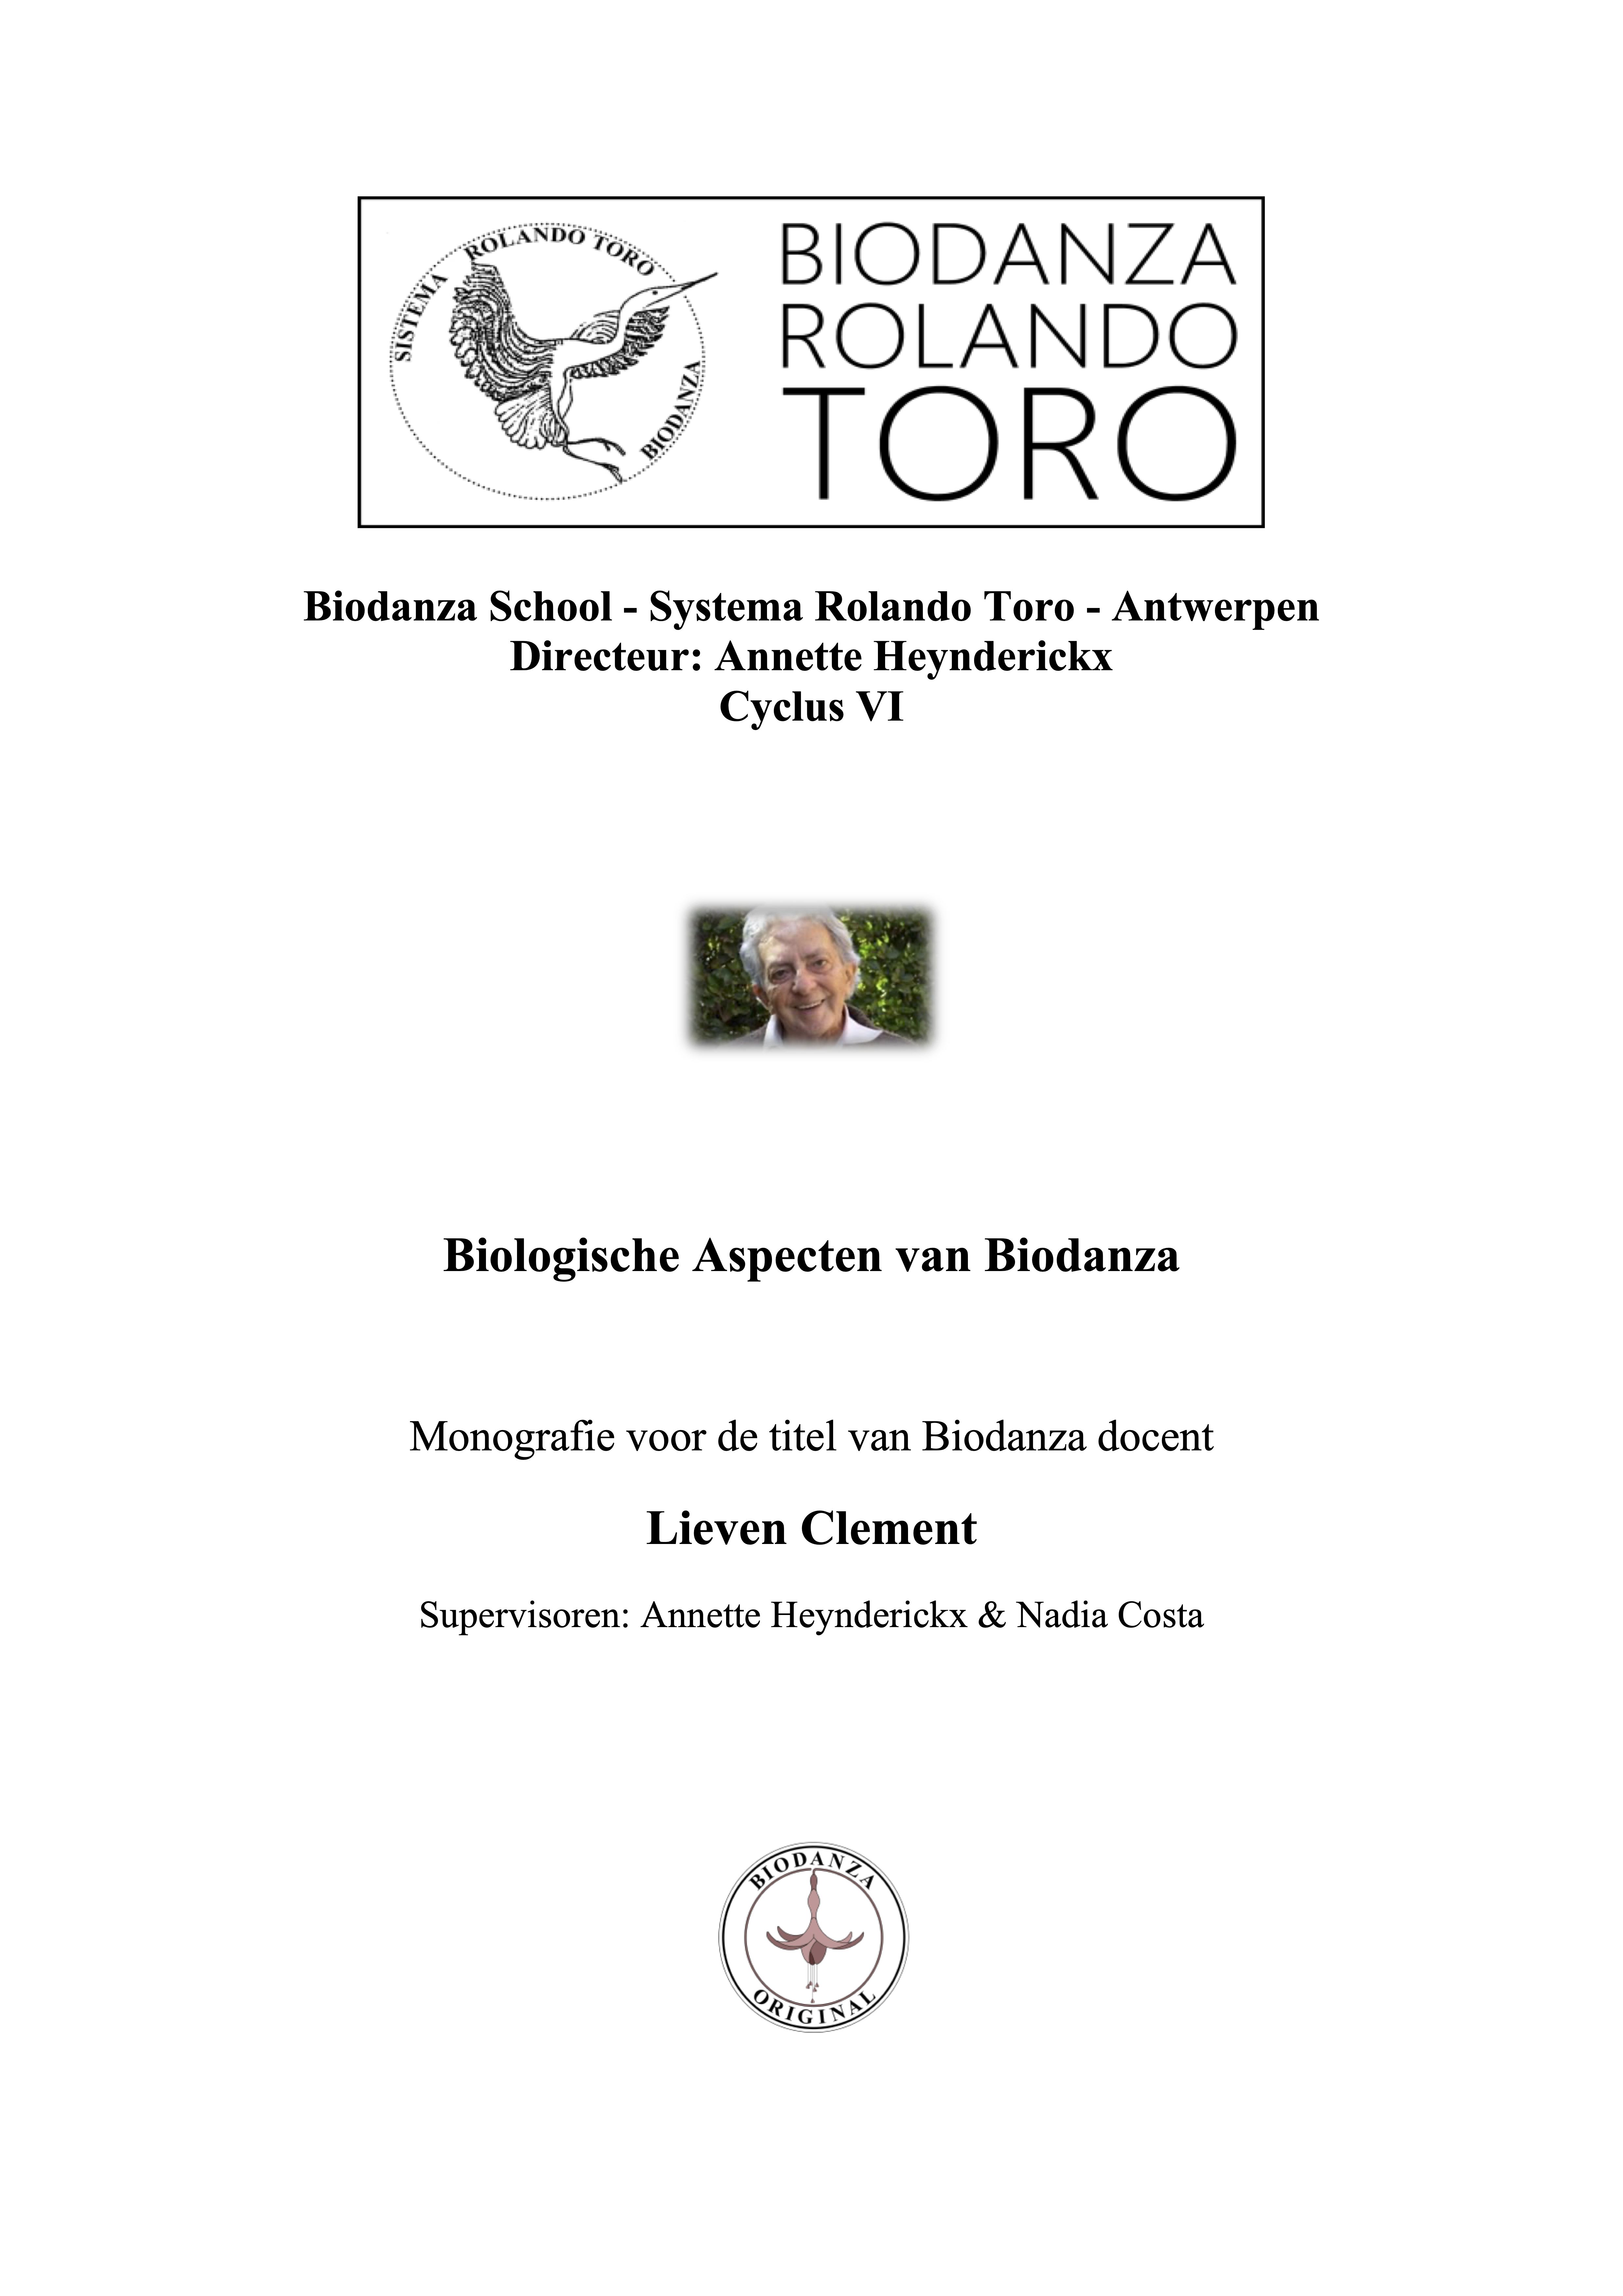
\includegraphics[width=1\linewidth]{./figs/titlePage} \end{center}
\newpage
\frontmatter
\pagenumbering{roman}
}

\usepackage[dutch]{babel}


\ifLuaTeX
  \usepackage{selnolig}  % disable illegal ligatures
\fi
\usepackage[]{natbib}
\bibliographystyle{apalike}
\IfFileExists{bookmark.sty}{\usepackage{bookmark}}{\usepackage{hyperref}}
\IfFileExists{xurl.sty}{\usepackage{xurl}}{} % add URL line breaks if available
\urlstyle{same} % disable monospaced font for URLs
\hypersetup{
  pdftitle={Biologische Aspecten van Biodanza},
  colorlinks=true,
  linkcolor={blue},
  filecolor={Maroon},
  citecolor={blue},
  urlcolor={blue},
  pdfcreator={LaTeX via pandoc}}

\title{Biologische Aspecten van Biodanza}
\author{}
\date{\vspace{-2.5em}}

\begin{document}
\maketitle

{
\hypersetup{linkcolor=}
\setcounter{tocdepth}{2}
\tableofcontents
}
\hypertarget{licentie-and-links}{%
\chapter*{Licentie and links}\label{licentie-and-links}}
\addcontentsline{toc}{chapter}{Licentie and links}

Deze monografie wordt gedeeld onder de CC BY-NC-SA 4.0 licentie op 26 February, 2024.

Het werk mag worden gebruikt voor niet-commerciële doeleinden.

Je bent vrij om het materiaal te kopiëren, te verspreiden en door te geven via elk medium of bestandsformaat. Om het te bewerken, te veranderen en afgeleide werken te maken. De gebruiker dient de maker van het werk te vermelden, een link naar de licentie te plaatsen en aan te geven of het werk veranderd is. Als je het werk hebt veranderd, of op het werk hebt voortgebouwd, moet je het veranderde materiaal verspreiden onder dezelfde licentie als het originele werk.

Een pdf versie van het eboek kan je hier vinden: \href{https://biodanzabrugge.be/biologischeAspectenBiodanza/Biologische-Aspecten-van-Biodanza.pdf}{Biologische-Aspecten-van-Biodanza.pdf}

An English version of this ebook can be found on: \href{https://biodanzabrugge.be/biologicalAspectsBiodanza/}{BiologicalAspectsBiodanza}

\mainmatter

\hypertarget{dankwoord}{%
\chapter*{Dankwoord}\label{dankwoord}}
\addcontentsline{toc}{chapter}{Dankwoord}

Mijn weg naar deze monografie is een pad van een heel leven.\\
Alles wat ik in me heb, kantelde hier finaal in samen.

Ik kwam ter wereld in een warm nest waar muziek door het huis vibreerde.\\
Een nest waar ik naast de passie voor muziek ook werd geprikkeld om na te denken en om mijn hersenspinsels woorden te geven.\\
Een nest die me ook de ruimte gaf om een passie voor wetenschap te ontwikkelen.

Toen ik achtien werd stond ik voor een keuze, wordt het muziek of wetenschap.\\
Het werd de wetenschap.\\
Die weg leidde me uiteindelijk tot mijn passie in statistical genomics, een tak van de statistiek die ons toelaat om uit massieve datasets te leren welke genen anders tot expressie komen als gevolg van interne en externe stimuli, ecofactoren, ziekte, ons genetisch potentieel, \ldots{}\\
Wat een belangrijke component zou blijken te zijn voor mijn begrip van het model van Biodanza.

Op dat wetenschappelijke pad was muziek naar de achtergrond verdwenen,\\
vergroeide ik langzaam aan steeds meer met mijn hoofd,\\
en werd mijn passie wat mechanisch door het Cartesiaanse denken die zo ruim verspreid is in de academische wereld.

Maar gelukkig was daar Fien.\\
Fien die me als een baken steeds weer naar het hier en nu wist te brengen.\\
Fien die me telkens weer toonde dat het leven zoveel meer is.\\
Fien die me het vaderschap leerde kennen en me drie zonen schonk.

Fien ook jij was het die uiteindelijk Biodanza op ons pad bracht,\\
waardoor weten voor mij weer voelen werd, en\\
hoofd en hart weer mochten gaan versmelten.

Biodanza die het beste in ons beiden naar boven brengt,\\
die ons samenzijn transformeert naar wat Rolando
het ecologische koppelzijn zou noemen,\\
omdat het onze sterktes smeedt tot een gedeelde passie,\\
tot een nieuwe manier van leven.

En zo bracht jij ook Annette \& Frank op mijn pad.\\
Eerst in je verhalen over de Biodanza opleiding die je volgde,\\
daarna door me mee te nemen naar hun Biodanza Stages in de Franse Ardennen,\\
en uiteindelijk door me helemaal te steunen om te starten in de nieuwe cyclus van de opleiding.

Een pad die me radicaal transformeerde.\\
Muziek, beweging, dans, passie, wetenschap, lichaam, geest,
het kwam allemaal weer samen en werd weer één.\\
Jullie lieten me ervaren hoe alles vertrekt vanuit het intens beleven van het leven, hier en nu.\\
Vivencia dus,\\
die me zijn gaan transformeren,\\
en dat is een kunst die jij Annette als geen ander verstaat\footnote{Een weerklank hiervan kan je terugvinden in het addendum van deze monografie}.

Naast vivencia, prikkelde je me in de opleiding ook door die vele wetenschappelijke concepten op me los te laten waarop Biodanza is gestoeld.
Die lieten de passie voor de wetenschap weer helemaal bij mij oplaaien.

En toen deed je iets onvoorstelbaars\ldots{}\\
Met een ongelofelijk vertrouwen
nodigde je me uit om samen de theorie van de Biologische Aspecten van Biodanza te brengen in de opleiding.\\
Iets die mijn transformatie helemaal in een stroomversnelling bracht en een jaar later uitkantelde in de eerste ruwe versie van deze monografie.

Een versie die ik Annemie en Frederieke heb laten lezen,
en waarvan ik, als ik er nu aan terug denk, licht begin te blozen.\\
Maar jullie feedback was essentiel om mijn schrijfsels beter af te stemmen op mijn doelpubliek.

Een half jaar later was het alweer jij, Annette,
die met een meesterzet het momentum nog maar eens zou gaan vergroten.\\
Het gebeurde aan jullie caravanneke
in het zuiden van Frankrijk.\\
Net voor de start van de extensie ``het pad van extase'' zette je mij en Fien samen met Nadia, een van de meest inspirerende personen die ik heb mogen ontmoeten\ldots{}\\
En je vroeg haar om mijn monografie te begeleiden.

En Nadia,\\
tijdens die extensie ging ik aan je lippen\ldots{}\\
Ieder woord resoneerde\ldots{}\\
Je spreekt de taal van het hart,\\
de taal van het leven\\
en dat met zoveel eenvoud en zo een diepgang.\\
En tussen de regels door
herkende ik ook zoveel van
de taal die me zo vertrouwd is,\\
die van de wetenschap.\\
En daarbovenop kwam nog eens de fenomenale taal van je beweging\ldots{}\\
Zo inspirerend.

In de maanden die kwamen heb je me met zo veel geduld en passie
meegenomen op de wandeling door mijn monografie.\\
Haarscherp wist je die te fileren,\\
te verdiepen,\\
en nog meer tot leven te wekken.

Iedere zoom-call was zo transformerend\ldots{}\\
Zelden was ik zo wakker, alert en helder.\\
Ieder woord telde\ldots{}\\
En telkens was er wel weer een nieuwe zin die dagen na bleef zinderen en de basis vormde van een volledig nieuwe call.

Je gaf me zoveel inzicht en vertrouwen.\\
Je nodigde me uit om te zoeken,\\
om de theorie van de biologische aspecten te doorvoelen, en\\
om die te verbinden met de methodologie van Biodanza.

En toen gaf je me je zegen om mijn monografie de wereld in te sturen,\\
maar niet zonder een laatste knipoog naar de rijkdom van Rolando's systeem:\\
``Et maintenant,\\
tu peux faire la même chose pour\\
les aspects fysiologiques,\\
les aspects psychologiques,\\
les prédécesseurs mythiques et philosophiques,\\
\ldots{}''

En tot slot wil ik iedereen nog bedanken waarmee ik heb mogen dansen.\\
In het bijzonder de mensen van de opleiding, en van onze maandag- en woensdag groep in Brugge.\\
Onze dansen hebben me gevormd, en\\
door jullie kan ik de schoonheid van het Biodanza-leraar-zijn ook gaan ontdekken\ldots{}

-- Februari 2024 --

\hypertarget{samenvatting}{%
\chapter*{Samenvatting}\label{samenvatting}}
\addcontentsline{toc}{chapter}{Samenvatting}

Ik begon in 2021 aan de lerarenopleiding Biodanza aan de School van Antwerpen. De verrijkte omgeving veranderde mijn kijk op het leven en hoe ik het leven ervaar volledig. Het zorgde voor een enorme persoonlijke groei en stimuleerde mij om mijn geest, lichaam en hart opnieuw te verbinden.

Tijdens de eerste module van de lerarenopleiding stond ik versteld om te zien dat de verticale as in het model van Biodanza zo nauw verweven leek te zijn met mijn wetenschappelijke pad van de afgelopen 25 jaar. Rolondo Toro werd bij de ontwikkeling van zijn Systeem van Biodanza door zoveel vooraanstaande wetenschappers geïnspireerd. Tijdens mijn formele wetenschappelijke opleiding kwam ik echter nooit in aanraking met veel van de concepten die in de eerste modules van de lerarenopleiding aan bod kwamen, en ik kon deze niet vatten zonder het werk van de oorspronkelijke auteurs te raadplegen.

Mijn monografie weerspiegelt dan ook mijn zoektocht om Rolando's visie op de biologische aspecten te begrijpen, die aan de basis liggen van zijn model van Biodanza. In het eerste hoofdstuk introduceer ik het model van Biodanza. In het tweede hoofdstuk probeer ik Rolando's kijk op het leven, zijn biocentrische principe en zijn concept ``vitaal onbewuste'' te verduidelijken. In dat hoofdstuk leg ik ook de basis voor de overige drie hoofdstukken die elk focussen op een belangrijk biologisch aspect in het model van Biodanza: (3) Principes van kosmisch leven en de ontstaansgeschiedenis van het leven, een kort verhaal over de geschiedenis van het universum tot aan de oorsprong van het leven, (4) Fylogenese en evolutie, waarin ik de geschiedenis van het leven en hoe het leven evolueerde kort introduceer, en (5) Ontogenese, waar ik toelicht hoe wij evolueren vanaf onze oorsprong van bevruchte eicel tot volwassenheid, totdat we uiteindelijk sterven. In het vijfde hoofdstuk ligt de nadruk sterk op epigenetica, de ontbrekende schakel die Rolando Toro nodig had om uit te leggen hoe Biodanza een verrijkte omgeving induceert die verandering teweegbrengt in hoe we ons genetisch potentieel gebruiken. Tenslotte sluit ik deze monografie af met enkele slotopmerkingen en met een addendum met enkele impressies die ik tijdens mijn Biodanza-lerarenopleiding heb geschreven.

\hypertarget{intro}{%
\chapter{Introductie}\label{intro}}

Mijn Biodanza-reis begon in 2018. Mijn vrouw Fien startte de opleiding tot Biodanza docent en samen sloten we ons aan bij een wekelijkse Biodanza-groep van Ann Vanhooreweder in Brugge. We voelden al snel de positieve impact van Biodanza op ons leven.

Twee jaar later vond er echte Biodanza-magie plaats. In januari 2019 kreeg onze oudste zoon een zwaar fietsongeluk, waarvan hij goed herstelde. Het transformeerde onze relatie als koppel echter tijdelijk tot een relatie ``van zorgen voor elkaar''. Begin 2020 realiseerden we ons dat de gebeurtenissen onze band enorm hadden verdiept, maar dat ten koste van passie en aantrekkingskracht. Het ``zorgen voor elkaar'' betekende dat we afwisselend in onze kracht gingen staan om de ander te ``containen'' waardoor onze emoties niet langer samenvielen. Ondanks onze inspanningen en dat we met ons hoofd ergens wisten wat er moest gebeuren, was het moeilijk om onze gevoelens weer op elkaar af te stemmen.

De Biodanza-magie overkwam ons op Annette's Biodanza vijfdaagse in de zomer van 2020. Die begon met een integrerende vivencia (Biodanza-sessie). De sleuteloefening van de vivencia was de ontmoeting. Zodra onze blikken kruisten, sloeg de emotie bij me binnen en zag ik dat Fien hetzelfde voelde. Het gebeurde in een oogwenk, hier en nu, en sindsdien hebben we onze emotionele resonatie hervonden\ldots{}

Hoe kan Biodanza zo transformerend zijn? Biodanza maakt gebruik van de kracht van muziek en beweging in een affectieve groep om vivencia op te roepen, een diepe ervaring met een sterke lichamelijke component. Vivencia gebeurt hier en nu en gaat ons mentale bewustzijn vooraf. Het kan positieve veranderingsprocessen op gang brengen die diep door kunnen werken in ons dagelijkse leven.

\begin{figure}

{\centering 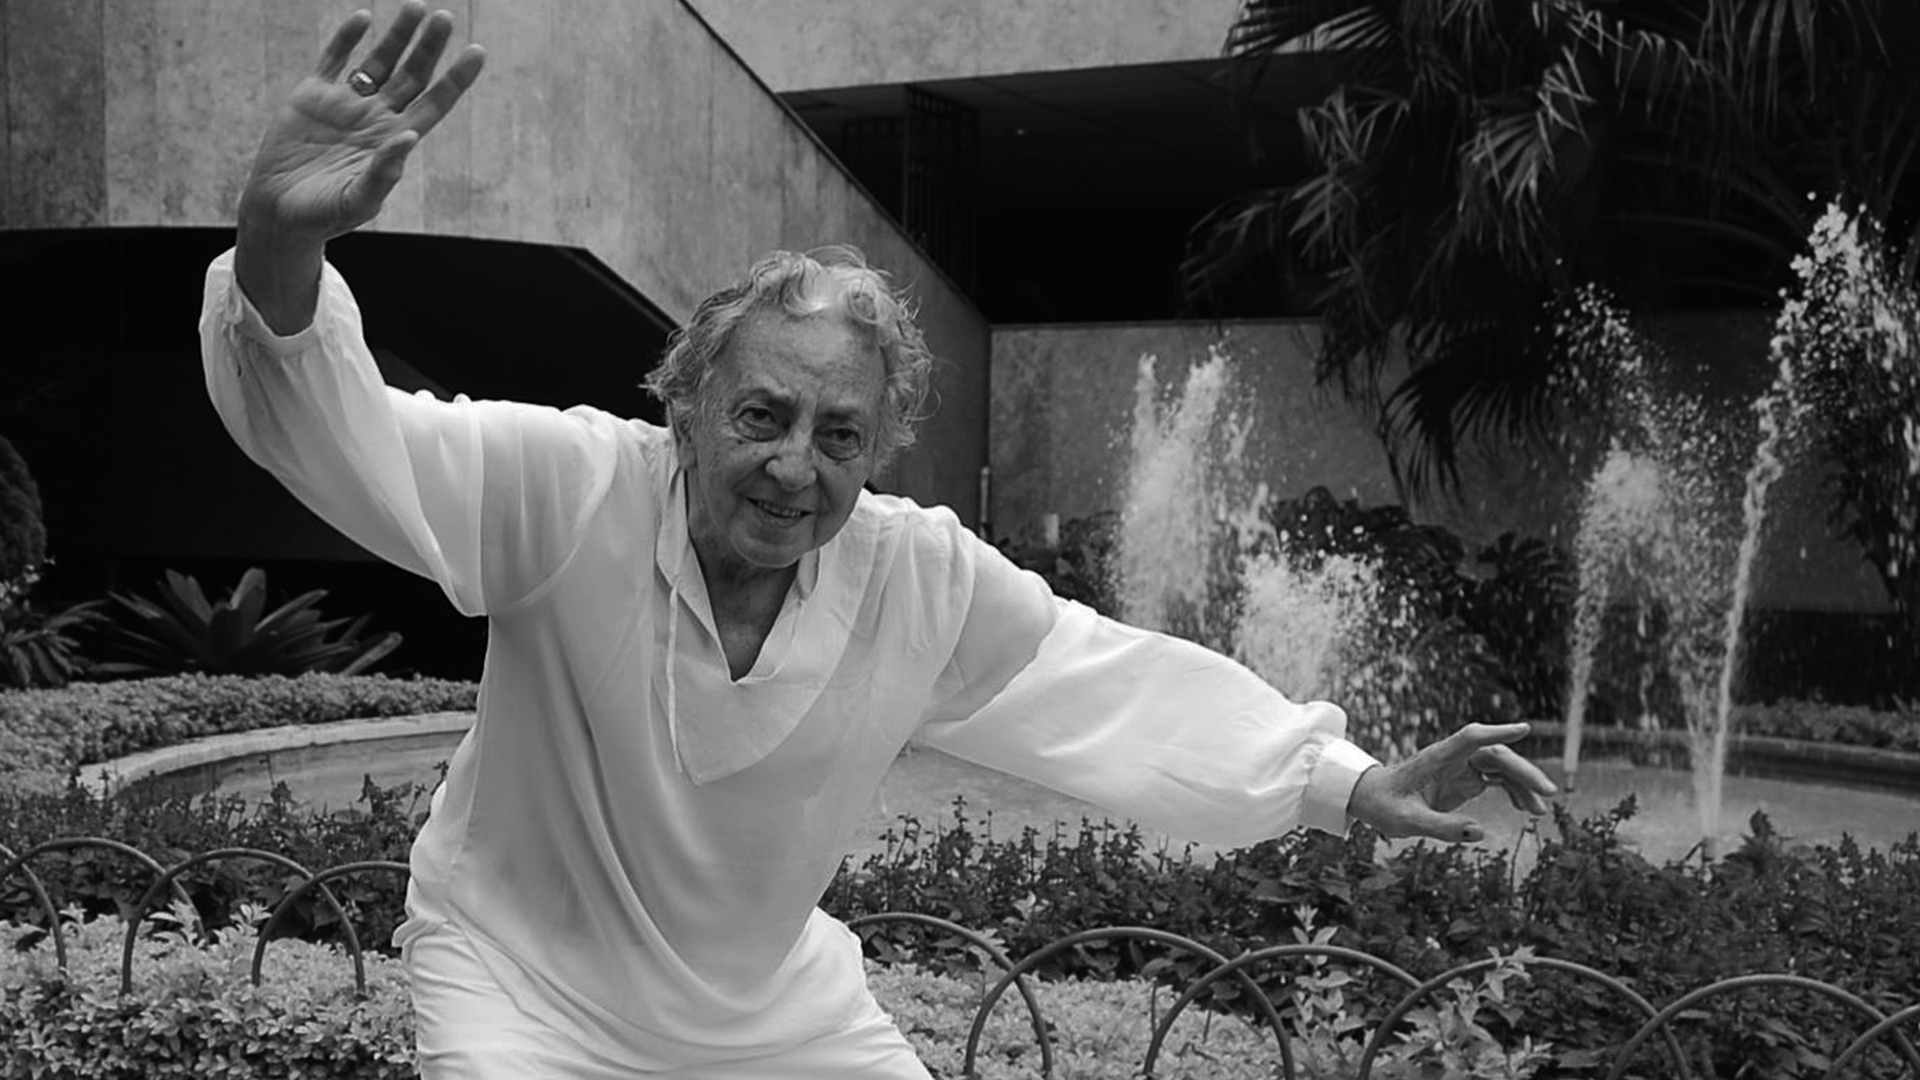
\includegraphics[width=0.45\linewidth]{./figs/rolando} 

}

\caption{Rolando Toro, de ontwikkelaar van Biodanza}\label{fig:rolandoToro}
\end{figure}

Voor Rolando Toro, die Biodanza ontwikkelde, was het meest belangrijke ``Vivencia, Vivencia, Vivencia''. Intens het leven ervaren door middel van dans, muziek en beweging waardoor we ons diep kunnen verbinden met onszelf, de ander en het groter geheel. Biodanza laat ons voelen dat het leven één is en dat door een diepe, intense lichamelijke beleving (vivencia).

Rolando Toro heeft het systeem van Biodanza ontwikkeld als antwoord op de degeneratie van de mens en de maatschappij die WOII voor hem blootlegde. Voor Rolando was het duidelijk dat de moderne mens lijdt aan de ``ziekte van de beschaving''. Die brengt ons zo ver van ons natuurlijke staat van zijn, van het voelen, affectie en inleven in de ander; waardoor ieder van ons tot extreme wreedheden kan worden bewogen.

Hij wilde daar een systeem van liefde en hoop tegenoverzetten. Een systeem waardoor er een affectieve heropvoeding mogelijk wordt en die de mens uitnodigt zich opnieuw te ontwikkelen in al zijn/haar schoonheid. Biodanza dus als systeem dat de mens wakker maakt om deel te nemen aan een nieuwe manier van leven en dat gevoed vanuit intense belevingen.

Rolando was een gepassioneerde wetenschapper en een professor in de psychologie. Hij ontwikkelde Biodanza vanuit zijn eigen ervaringen en dat diep ingebed in de levenswetenschappen. Hij werd ook enorm geïnspireerd door de grondleggers van de moderne dans en door oervolkeren die een diepe betekenis leggen in elke beweging. Als we als mens leren om weer betekenis toe te voegen aan onze bewegingen, gaan we weer doorleefd in het leven staan, verbonden met al wat is.

\begin{figure}

{\centering 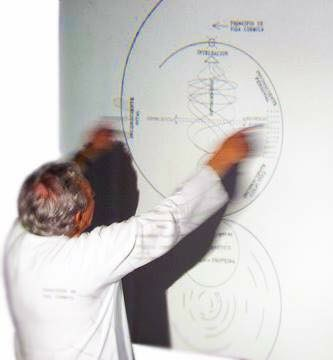
\includegraphics[width=0.45\linewidth]{./figs/rolandoAndModel} 

}

\caption{Rolando Toro legt zijn Biodanza-Model uit}\label{fig:rolandoModel}
\end{figure}

Rolando heeft de basis van zijn systeem gelegd tijdens zijn loopbaan als psycholoog/onderzoeker waar hij de grote impact ontdekte van oefeningen die identiteit en biologische regressie stimuleren, de eerste as van zijn systeem. In tegenstelling tot de klassieke visie van de psychiatrie die symptomatisch werkt en medicijnen toedient, ontwikkelde Rolando de visie om het lichaam door middel van externe stimuli (ecofactoren), zoals muziek, beweging, aanraking en dans, te stimuleren om deze stoffen eenvoudigweg zelf intern aan te maken. Op die manier worden we gestimuleerd om onszelf te herbalanceren, om te groeien en om de informatie in ons genetisch potentieel opnieuw aan te boren.

Groei en leren gebeurt in Biodanza zoals bij kinderen: door te zien, te imiteren, te beleven en door herhaling, en dat diep ingebed in een verrijkte omgeving met positieve bekrachtiging.

In het vervolg van dit hoofdstuk zullen we de basis leggen die nodig is om ons te kunnen verdiepen in de biologische aspecten van Biodanza. We beginnen met de definitie van Biodanza. We gaan verder met Rolando's Biocentrische Principe. Vervolgens introduceren we het Biodanza-Model en sluiten we af met de doelstellingen van deze monografie.

\hypertarget{definitie-van-biodanza}{%
\section{Definitie van Biodanza}\label{definitie-van-biodanza}}

Rolando bedacht de term ``Biodanza'', wat een samentrekking is van ``bios'', het Griekse woord voor ``leven'', en ``danza'', het Spaanse woord voor dans. Hierbij wordt het woord ``danza'' gebruikt in zijn oorspronkelijke betekenis van ``natuurlijke beweging'' die vol is van betekenis en dat sterk verbonden met onze emoties.

Rolando Toro definieerde Biodanza als de poëzie van de ontmoeting. Alle oefeningen kunnen inderdaad worden gezien als een voorbereiding op de ontmoeting met jezelf, de ander en het groter geheel.

In Rolando's meer academische definitie is Biodanza een systeem van menselijke integratie, van organische vernieuwing, van affectieve heropvoeding en van het opnieuw leren van de oorspronkelijke functies van het leven.

De methodologie van Biodanza bestaat uit het induceren van integrerende vivencia door middel van muziek, beweging en ontmoetingen in een affectieve groep.

In 2009 werkte hij zijn definitie als volgt bij: ``Biodanza is een systeem dat integratieve processen versnelt op cellulair, immunologisch, metabolisch, neuro-endocrino en existentieel niveau door een verrijkte omgeving te bieden met geselecteerde muziek, integratieve beweging, strelingen en groepsinteracties.''

In de onderstaande secties leggen we de verschillende delen van de definitie uit.

\hypertarget{vivencia}{%
\subsection{Vivencia}\label{vivencia}}

Het concept vivencia is essentieel om de methode van Biodanza te begrijpen.

Vivencia is een intense sensatie van leven, hier en nu, met een sterke lichamelijke component. Het is een manifestatie van het zijn die aan ons mentale bewustzijn voorafgaat. Vivencia zijn voorbijgaande ervaringen, bijvoorbeeld de vivencia van volheid, van veiligheid, van vreugde. Het besef van het ervaren van vivencia kan onmiddellijk plaatsvinden of op een later moment en kan aanleiding geven tot diepe emoties.

We hoeven onze vivencia niet te rationaliseren. Ze kunnen worden gezien als manifestaties van onze lichamelijke wijsheid en brengen spontaan integratie en leren door ervaring op gang. Het zijn transformerende ervaringen, die de essentie vormen van de methode van Biodanza. Onze vivencia zijn inderdaad van cruciaal belang voor groei en integratie. Het beoefenen van Biodanza kan ook een gevoel van ontwaken teweegbrengen als we merken dat er groei heeft plaatsgevonden na de integratie van onze vivencia.

\hypertarget{menselijke-integratie}{%
\subsection{Menselijke Integratie}\label{menselijke-integratie}}

Door vivencia wordt een sterke verbinding met het leven tot stand gebracht, die de integratie met jezelf, de menselijke soort en het universum versterkt.

De integratie met onszelf herstelt onze psycho-fysieke eenheid, d.w.z. de eenheid van de interne/psychische en externe/fysieke wereld.

Integratie met de anderen herstelt de verbinding met onze menselijke soort, onze biologische eenheid.

Integratie met het universum herenigt ons met de natuur en herstelt onze intieme relatie met de hele biosfeer. Het laat ons opnieuw de diepe verbondenheid van onszelf als onderdeel van de kosmos ervaren.

Door deze verbinding met het leven te herstellen, kunnen we de kern van het leven opnieuw ervaren, hier en nu, wat groei en vernieuwing op biologisch, fysiologisch en psycho-emotioneel vlak bevordert en ook gepaard kan gaan met een gevoel van een diepe bewustwording.

\hypertarget{organische-vernieuwing}{%
\subsection{Organische Vernieuwing}\label{organische-vernieuwing}}

Biologische systemen bezitten het unieke vermogen tot zelfreplicatie en zelforganisatie. Stress kan een diepgaande invloed hebben op het onderhoud en de regeneratie van onze cellen en weefsels.

Met transcendente Biodanza-oefeningen vertragen we onze bewegingen, verlagen we onze staat van controle en roepen we een diepe staat van rust op. Deze toestand is essentieel om herstel en regeneratieprocessen op gang te brengen. Het versterkt de homeostase, het mechanisme van ons lichaam om zijn evenwicht te behouden ondanks de veranderingen in onze omgeving.

\hypertarget{affectieve-heropvoeding}{%
\subsection{Affectieve Heropvoeding}\label{affectieve-heropvoeding}}

In Biodanza stimuleren veel oefeningen genegenheid en harmonie, die in ons dagelijks leven kunnen doorwerken door harmonie te brengen in onze relatie met onszelf, met elkaar en met onze omgeving.

\hypertarget{herleren-van-de-oorspronkelijke-functies-van-het-leven}{%
\subsection{Herleren van de Oorspronkelijke Functies van het Leven}\label{herleren-van-de-oorspronkelijke-functies-van-het-leven}}

Het beoefenen van Biodanza brengt ons ook opnieuw in contact met onze oerinstincten, die in onze moderne samenleving sterk onderdrukt worden en vaak als irrationeel gedrag worden bestempeld. Onze instincten kunnen echter worden gezien als de biologische wijsheid van onze soort, die is geëvolueerd voor de overleving en instandhouding van onze soort. Door ons opnieuw te verbinden met onze aangeboren impulsen, herstellen we ook de harmonie van binnenuit.

\hypertarget{verrijkte-omgeving}{%
\subsection{Verrijkte omgeving}\label{verrijkte-omgeving}}

Biodanza biedt een verrijkte omgeving met een diep respect voor de uniciteit van elk individu, zonder oordeel en zonder te vergelijken. Een omgeving die de groei en vrije expressie van elke deelnemer in de groep stimuleert. De verrijking komt ook voort uit geselecteerde muziek, integratieve beweging, streling en groepsinteracties die als positieve ecofactoren werken. Een ander cruciaal element is de structuur en herhaling die wordt geboden door de wekelijkse Biodanza-lessen. De wekelijkse vivencia zijn progressief en transformerend. Ze versnellen de menselijke integratie op fysiek, fysiologisch, psychologisch, emotioneel, sociaal en existentieel vlak.

\hypertarget{sectionBiocentricPrinciple}{%
\section{Biocentrisch Principe}\label{sectionBiocentricPrinciple}}

Het Biocentrische Principe is het axioma waarvan Rolando Torro's systeem van Biodanza vertrekt. Vanuit het Biocentrische Principe beschouwt men het universum als de matrix van het leven, d.w.z. een zelforganiserende structuur die het leven opbouwt. Dus niet alleen levende organismen, maar de hele kosmos kunnen worden gezien als een gigantisch levend hologram.

Deze visie nodigt mensen uit om hun relatie tussen de mens en de biosfeer radicaal te herdenken. Vanuit dat uitgangspunt is het leven intrinsiek sacraal wat ons er toe aanzet om niet langer de mens maar alle leven, en dus het hele universum, centraal te zetten.

Mij lijkt het dus een uitnodiging om vanuit het antropocentrisme, met de mens als middelpunt, terug te keren naar de visie van oerculturen waarin de omgeving waarin we leven niet langer wordt gezien als het toneel waarop we ons bewegen, maar als een entiteit waar we mee kunnen communiceren en een intieme relatie mee op kunnen bouwen.

Vivencia is de unieke weg om het Biocentrische Principe te ervaren en hiervan te worden doordrongen.

\hypertarget{sectionModelOfBiodanza}{%
\section{Biodanza-Model}\label{sectionModelOfBiodanza}}

Rolando Toro ontwikkelde een schematische voorstelling van zijn Biodanza-Model. Het vat de wetenschappelijke basis en de methodologie samen, en wordt weergegeven in Figuur \ref{fig:model}.

\begin{figure}

{\centering 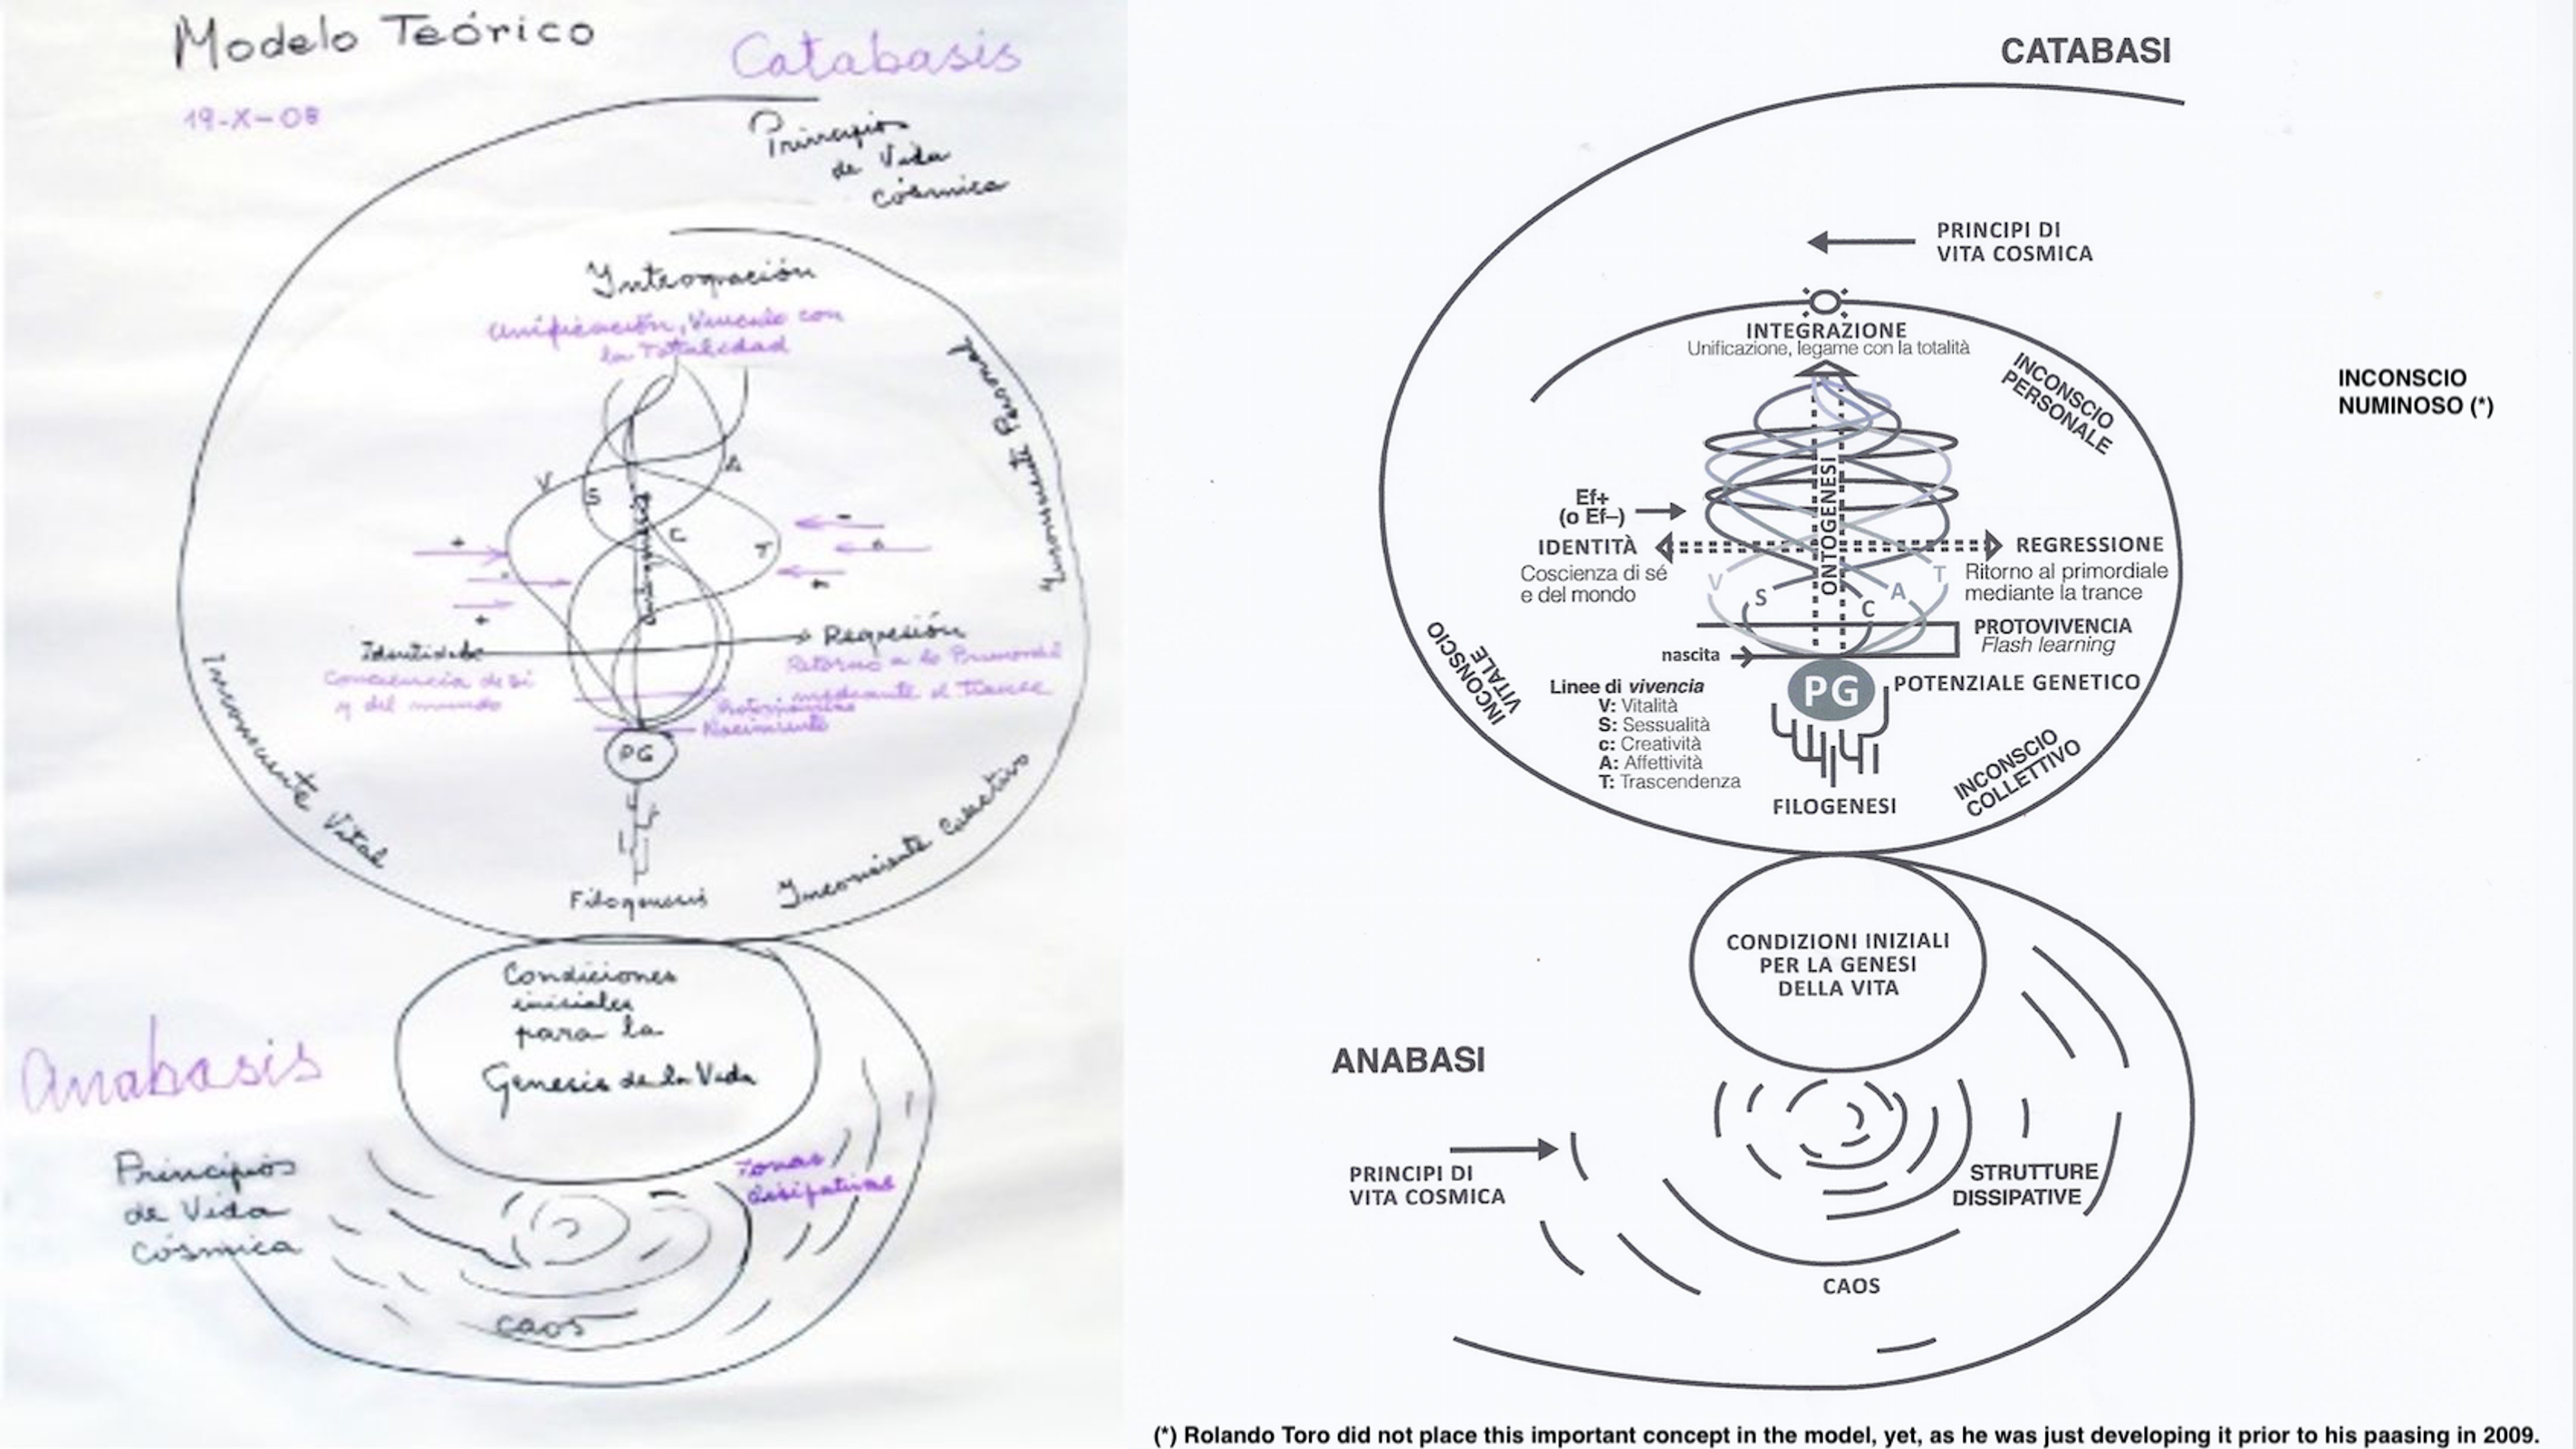
\includegraphics[width=1\linewidth]{./figs/biodanzamodel2andRolando} 

}

\caption{Biodanza-Model (links: getekend door Rolando Toro in 2008, rechts: versie van op de AIPOB website die ik heb aangepast)}\label{fig:model}
\end{figure}

In deze sectie zal ik eerst kort de biologische aspecten introduceren in het Biodanza model wat het hoofdthema is van deze monografie. Vervolgens zal ik kort ingaan op de methodologie van Biodanza.

\hypertarget{biologische-aspecten-van-biodanza}{%
\subsection{Biologische Aspecten van Biodanza}\label{biologische-aspecten-van-biodanza}}

In Figuur \ref{fig:model} zien we dat de biologische aspecten van Biodanza de vertikale as vormen van het Biodanza-model. Merk op dat deze concepten ook een belangrijke sociale, psychologische, emotionele en mystieke dimensie hebben aangezien een groot deel van ons menselijke leven zich afspeelt in het sociaal-symbolisch domein.

De vertikale as bestaat uit

\begin{enumerate}
\def\labelenumi{\arabic{enumi}.}
\tightlist
\item
  De principes van het kosmische leven en de genese\footnote{ontstaan} van het leven
\item
  Evolutie and fylogenese
\item
  Genetisch potentieel and ontogenese
\end{enumerate}

Deze verticale as wordt aangedreven door het symbiotische paar anabasis/katabasis, oftewel creatie/vernietiging. Anabasis is de integratie van chaos tot zelforganiserende systemen, zoals levende wezens, terwijl katabasis verwijst naar de desintegratie van dergelijke systemen. In de desintegratie ligt echter onmiddellijk de kiem voor nieuwe leven verscholen. Het leven is inderdaad inherent cyclisch.

Onze kosmos zoals wij die kennen is ontstaan uit chaos. Het begon vanuit een heel energierijke staat. Het koelde geleidelijk af waarbij energie in massa werd omgezet: het merendeel in waterstof, het lichtste element, en een fractie in de iets zwaardere heliumkernen. Door de zwaartekracht begon de materie zich vervolgens in nevels te clusteren waaruit uiteindelijk sterren zijn gevormd.

In de sterren zijn alle andere elementen (helium, koolstof, zuurstof, stikstof, enz.) gevormd uit waterstof door kernfusie en bij elke supernova, d.w.z. een explosie van een ster aan het einde van zijn leven, worden deze elementen/atomen in de ruimte gekatapulteerd.

In de ruimte reageerden deze atomen verder en vormden ze meer complexe moleculen die uiteindelijk leidden tot de precursoren (``voorlopers'') van de biologische bouwstenen van het leven. Alles om ons heen en ook wijzelf zijn dus opgebouwd uit sterrenstof.

In een uithoek van onze Melkweg, een modaal sterrenstelsel, op een modale planeet, de Aarde, waren er unieke omstandigheden die het ontstaan van biologisch leven mogelijk maakten. Eerst was er een chemisch evolutionair proces waaruit moleculen met toenemende complexiteit zijn ontstaan die zelfreplicatie en zelforganisatie mogelijk maakten. Daaruit de vier essentiële biomoleculen zijn ontstaan waaruit elk biologisch organisme is opgebouwd:

\begin{itemize}
\tightlist
\item
  Lipiden of vetten die worden gebruikt voor de opslag van energie en ook de vorming mogelijk maken van membranen die de binnenkant van de cel scheiden van de buitenwereld,
\item
  Koolhydraten of suikers die worden gebruikt als energiebron/bron en als ruggengraat van veel biomoleculen,
\item
  Eiwitten, de werkpaarden in onze cellen die de meeste chemische reacties in onze cellen mogelijk maken, en
\item
  Nucleïnezuren, DNA en RNA, die worden gebruikt om ons genoom, d.w.z. de set van genen die we van onze ouders hebben geërfd op te slaan, door te geven en af te lezen.
\end{itemize}

Toen de eerste levende cellen eenmaal verschenen, begonnen ze te evolueren. Door die evolutie brachten ze alle andere levende wezens voort. Dit proces wordt ook wel fylogenese genoemd.

Wij mensen zijn uiteindelijk een blad aan een kleine zijtak van de levensboom. Ieder van ons met zijn eigen genetische potentieel. In de loop van ons leven ontwikkelen we ons van een bevruchte eicel naar een embryo, een kind, een volwassene, totdat we uiteindelijk sterven. Tijdens dit proces, ook wel ontogenese genoemd, verandert de manier waarop we onze genen gebruiken.

Bij de conceptie erven we namelijk de structuur van onze cellen van de eicel van onze biologische moeder en ons genoom van onze biologische moeder en vader. In het begin heeft deze eicel toegang tot al onze genen. Maar naarmate de cel zich deelt beginnen groepen cellen zich in verschillende weefsels te differentiëren. Deze meer gespecialiseerde cellen hebben slechts toegang tot een beperkt aantal genen die essentieel zijn voor hun functie. Dit gebeurt via kleine moleculen die interageren met ons DNA en genen aan of uit kunnen zetten. De studie van hoe onze ontwikkeling, ons gedrag en onze omgeving veranderingen kunnen veroorzaken die een invloed hebben op hoe we onze genen kunnen gebruiken, wordt ook wel epigenetica genoemd.

Epigenetische veranderingen worden bij de celdeling doorgegeven aan de twee nieuwe cellen die worden gevormd, waardoor een levercel na celdeling een levercel blijft en een hersencel na celdeling een hersencel blijft.

Ook externe stimuli en ecofactoren kunnen epigenetische veranderingen veroorzaken.
Daarmee beïnvloeden ze dus de manier waarop we ons genetisch potentieel gebruiken.
Merk op dat ontogenese in zijn bredere definitie niet alleen kijkt naar de pure biologische ontwikkeling van het individu, aangezien die ontwikkeling ook belangrijke sociale, psychologische en emotionele implicaties heeft. Het was precies in dit grotere gebied dat Rolando actief was. Een vakgebied dat op het snijvlak ligt van de levenswetenschappen, antropologie, psychologie, fysiologie, kunst en mystiek, en van waaruit hij zijn Biodanza-systeem voor groei en integratie ontwikkelde.

\hypertarget{methodologie-van-biodanza}{%
\subsection{Methodologie van Biodanza}\label{methodologie-van-biodanza}}

Vivencia is de hoeksteen van de methode van Biodanza. Het verbindt ons opnieuw met de essentie van het leven en blijft dikwijls zowel op psycho-socio-emotioneel als op fysiologisch niveau doorwerken. Wanneer we een diepe vivencia ervaren, gaat dit gepaard met intense lichamelijke sensaties. Een Biodanza-sessie kan dus fysiologische veranderingen teweegbrengen en de productie van hormonen, neurotransmitters en eiwitten op gang brengen, die voortkomen uit de expressie van specifieke genen in ons lichaam en onze hersenen.

Door onze vivencia te integreren, het herhalen van oefeningen en de structuur van de wekelijkse lessen, kan Biodanza menselijke groei en evolutie bevorderen. Mensen die Biodanza voor langere tijd beoefenen, ervaren dat het een diepe impact kan hebben op hun leven en hun sociale interacties. Merk op dat dit ook gepaard kan gaan met veranderingen op biologisch-fysiologisch niveau. Ecofactoren kunnen inderdaad epigenetische veranderingen teweegbrengen die de expressie van genen activeren of blokkeren, en ze kunnen ook (nieuwe) neurale verbindingen induceren en/of versterken. Het beoefenen van Biodanza kan dus de expressie van ons genetisch potentieel beïnvloeden.

De methodologie van Biodanza staat centraal in het Biodanza-Model, zie Figuur \ref{fig:model}.

\hypertarget{muziek-beweging-en-vivencia}{%
\subsubsection{Muziek, Beweging en Vivencia}\label{muziek-beweging-en-vivencia}}

Vivencia wordt opgeroepen door middel van muziek, beweging en ontmoetingen in een affectieve groep.

Muziek is een universele taal en een zeer krachtige bron van transformatie. In Biodanza heeft het een essentiële functie: het oproepen van vivencia. Daarom worden de muziekstukken die in Biodanza worden gebruikt zeer zorgvuldig gekozen op basis van hun emotionele inhoud, de organische effecten die ze bevorderen en het soort vivencia dat ze oproepen; voordat ze aan het Biodanza-repertoire worden toegevoegd \citep{toro2008}.

Beweging is een andere universele taal die transformerend kan zijn en ook een sleutelfunctie speelt bij het oproepen van vivencia. Daarom worden de bewegingen bij Biodanza-oefeningen ook zeer zorgvuldig gekozen. Ze komen voort uit natuurlijke bewegingen van mensen, gebaren die worden gebruikt bij `socialiserende rituelen', zoals het geven van handen, omhelzen, strelen, enz.; en archetypische gebaren, die we ook terugvinden in de kunst van alle menselijke culturen en tradities. De bewegingen kunnen door iedereen worden uitgevoerd. Hun verfijning komt echter voort uit de betekenis, emotie en gevoel die de deelnemer erin legt, die van cruciaal belang is voor de diepgang van de vivencia \citep{toro2008}.

Muziek, beweging en vivencia vormen dus een gestalt. Een kleine verandering in één onderdeel kan de vivencia die ontstaat radicaal veranderen. Met de delicate keuze van de volgorde van Biodanza-oefeningen, de volgorde van vivencia, ontvouwt zich een overkoepelende vivencia voor de hele sessie.

Biodanza kan niet worden beoefend in isolatie. De ontmoeting met elkaar is een essentieel onderdeel van de beweging en voor het genereren van een veld dat de integratie met jezelf, met onze menselijke soort en het groter geheel mogelijk maakt.

\hypertarget{horizontale-as-identiteit-en-biologische-regressie}{%
\subsubsection{Horizontale As: Identiteit en Biologische Regressie}\label{horizontale-as-identiteit-en-biologische-regressie}}

Rolando heeft de basis van zijn systeem gelegd tijdens zijn carrière als psycholoog/onderzoeker, waar hij de impact ontdekte van oefeningen die identiteit en biologische regressie stimuleren, de horizontale as in zijn systeem.

Een Biodanzasessie begint doorgaans met vitale ritmische oefeningen die de deelnemers bewust maken van hun lichaam en hun identiteit. Vervolgens maken we de brug naar meer verdiepende oefeningen waarbij we onze bewegingen vertragen om onze staat van controle te verlagen. Dit kan een diepe staat van rust, oplossen van ons ego, transcendentie en integratie oproepen. Een staat van biologische regressie die harmonieus en progressief is, die belangrijke fysiologische patronen reactiveert en ons in contact brengt met onze oorsprong en ons potentieel om onszelf opnieuw te herbalanceren. In Biodanza verwijst regressie altijd naar deze belangrijke staat van biologische regressie.

\hypertarget{verticale-as-vijf-lijnen-van-biodanza}{%
\subsubsection{Verticale As: Vijf Lijnen van Biodanza}\label{verticale-as-vijf-lijnen-van-biodanza}}

Rolando structureerde ons genetisch potentieel in vijf lijnen: vitaliteit, seksualiteit, creativiteit, affectiviteit en transcendentie. Ze vormen zijn vertaling van het biologische concept van ons genetisch potentieel naar een breder biologisch en socio-psycho-emotioneel domein waarin menselijke groei en ontwikkeling plaatsvindt. In een Biodanzasessie werken we doorgaans in twee of meer van deze lijnen.

In het model draaien de vijf lijnen spiraalvormig rond de verticale as van de ontogenese. Wekelijkse Biodanza-sessies leveren inderdaad de ecofactoren aan die groei in deze vijf lijnen induceren en die langdurige effecten kunnen hebben op genomisch, fysiologisch en psycho-socio-emotioneel vlak.

We worden al heel vroeg in ons leven blootgesteld aan deze vijf lijnen, wat Rolando protovivicencia noemde. Protovivencia zijn de ervaringen van een pasgeborene als reactie op interne en externe stimuli, zoals aandacht, voedsel, liefde, zorg en strelingen.

De protovivencia gaat hand in hand met ``flash-learning'', het zeer snelle leren dat plaatsvindt in de eerste zes maanden van een pasgeborene. Deze protovivencia kunnen ook worden gestructureerd volgens de vijf lijnen van Biodanza. Zoals Rolando beschreef in zijn boek Biodanza \citep{toro2008} komt de protovivencia van vitaliteit voort uit beweging, actie en rust; de protovivencia van de seksualiteit wordt geïnduceerd door contact en liefkozingen; die van creativiteit door expressie en nieuwsgierigheid; die van affectiviteit door voeding en bescherming; en die van transcendentie door de harmonie die een kind ervaart met zijn omgeving.

Tijdens een Biodanza-sessie laten we (een deel van) de vijf lijnen pulseren door een serie van oefeningen waarvan de eerste onze identiteit versterken en de daaropvolgende oefeningen biologische regressie progressief stimuleren. Oefeningen die de identiteit versterken zorgen ervoor dat deelnemers zich bewuster worden van zichzelf, de wereld om hen heen en hoe zij in die wereld staan. Oefeningen die biologische regressie stimuleren, stimuleren daarentegen het oplossen van ons ego en om ons te verbinden met de verschillende niveaus van ons onbewuste.

\hypertarget{onbewuste}{%
\subsubsection{Onbewuste}\label{onbewuste}}

In de periferie van de methodologie van Biodanza in het Model (Figuur \ref{fig:model}) vinden we het persoonlijk onbewuste, het collectief onbewuste en het vitaal onbewuste. Dat is een resonantie met respectievelijk ideeën en informatie over onszelf, onze oerinstincten en archetypen, en de informatie die pulseert in de matrix van het leven.

Wanneer een vader zijn baby streelt, maakt hij verbinding met zijn persoonlijk onbewuste door de band die hij ervaart met zijn kind, met het Demeter- of moederarchetype in zijn collectief onbewuste, en met zijn vitaal onbewuste door de fysiologische reactie die hij ervaart via de eiwitten, hormonen en neurotransmitters die in zijn cellen tot expressie komen.

Veel van onze acties worden gestuurd door ons onbewuste. Door middel van Biodanza-oefeningen die gericht zijn op biologische regressie en transcendentie kunnen we ons diep verbinden met deze drie soorten onbewuste.

Aan het eind van zijn leven introduceerde Rolando Toro een vierde onbewuste, een diepere onbewuste, een oeronbewuste die ons menselijk maakt, een onbewuste van de menselijke grootsheid: het numineus onbewuste. Het is volgens Rolando het meest onderdrukte onbewuste. Een onbewuste dat onderdrukt wordt door onze cultuur en haar fatale dissociaties die ons kleiner en onbeduidend maken \citep{toro2009}.
Het numineus onbewuste bestaat uit vier sleutelkenmerken: liefde, verlichting, moed en intase. De behoefte om lief te hebben is inderdaad inherent aan ons organisme. Liefde impliceert gemeenschap, empathie, tederheid en barmhartigheid. Het kan ongedifferentieerd zijn: liefde voor de mensheid, of gedifferentieerd: liefde voor een bepaalde persoon of groep. Het kan zelfs een kosmisch niveau bereiken, de epifanische liefde, waarin ons hart in gemeenschap treedt met het hart van de ander. Het tweede kenmerk is verlichting. Verlichting niet als dat van een goeroe, maar als een proces naar de ander toe. Het is het vermogen om het beste in ieder van ons te zien, hun essentie te ontdekken en hun verlangen om te leven en gelukkig te zijn te onthullen. Het derde kenmerk is moed. De moed om zonder angst te weten wat we willen, om onze angst om te leven en lief te hebben uit te dagen. De moed om uit de chaos op te staan als we lijden of ons in de steek gelaten voelen. Het vierde kenmerk is intase. Dat verwijst naar de pracht van onze soort en de pracht van deel uit te maken van het universum, van de kosmos \citep{toro2009}.
\newpage 

\hypertarget{doelstellingen-van-deze-monografie}{%
\section{Doelstellingen van deze Monografie}\label{doelstellingen-van-deze-monografie}}

Deze monografie focust op de biologische aspecten van Biodanza. Het is mijn impressie van ``Module II: Vitale Onbewustzijn en Biocentrisch Principe'' en ``Module IV: Biologische Principes van Biodanza'' van de Opleiding tot Biodanza Docent die ik volgde aan de School van Antwerpen.

Ik zal proberen om alle concepten die voorkomen in het officiële leermateriaal van deze twee modules in de context van het Biodanza-Model te plaatsen. Het is mijn bescheiden poging om meer inzicht te geven in deze biologische aspecten voor Biodanza-leraren en -liefhebbers die dieper in de wetenschappelijke achtergrond van het Systeem van Biodanza willen duiken.

Het bestaat uit vier delen:

\begin{enumerate}
\def\labelenumi{\arabic{enumi}.}
\item
  ``Wat is leven'', waarin ik een fundament leg en belangrijke biologische concepten introduceer die een dieper inzicht kunnen verschaffen in de twee concepten: het Biocentrisch Principe en het Vitaal Onbewuste.
\item
  ``Principes van het kosmische leven en de genese van het leven'', een kort verhaal over de geschiedenis van het universum tot aan de oorsprong van het leven.
\item
  ``Evolutie and Fylogenese'', dat gaat over de geschiedenis van het leven en hoe het leven evolueerde.
\item
  ``Ontogenese'', waar ik mijn licht werp op hoe we evolueren van onze oorsprong als bevruchte eicel naar volwassenheid toe totdat we uiteindelijk sterven.
\end{enumerate}

Hoewel de rest van deze monografie zich richt op de biologische aspecten van Biodanza, is het echter belangrijk om in gedachten te houden dat het niet mijn bedoeling is om het Biodanza-Model te reduceren tot de biologische aspecten. Veel van de concepten die we vanuit biologisch perspectief zullen bespreken, hebben ook een belangrijke sociologische, psychologische, emotionele en mystieke dimensie, aangezien een substantieel deel van ons menselijk leven zich afspeelt in het sociaal-symbolische domein.

\hypertarget{wat-is-leven}{%
\chapter{Wat is Leven?}\label{wat-is-leven}}

Een van de belangrijkste drijfveren voor Rolando Toro om zijn Systeem van Biodanza te ontwikkelen was zijn observatie dat we als westerse mens niet meer verbonden zijn met onze oorsprong en met de kosmos, wat destructieve culturele vormen heeft voortgebracht. Deze komen voort uit onze cartesiaanse manier van denken en zorgde voor een gefragmenteerde kijk op het leven. Dat denken impliceert inderdaad een scheiding tussen lichaam en geest, mens en natuur, levende materie en niet-levende materie, en het bestudeert het universum alsof het uit afzonderlijk bestaande delen bestaat die min of meer op elkaar inwerken als delen van een machine \citep{bohm1980}. Ons gefragmenteerde wereldbeeld heeft ons ontgekoppeld van de kosmische matrix; onze samenleving opgedeeld in verschillende religieuze, politieke, economische en raciale groepen; en leidde tot de roofbouw op de natuur, planten, dieren en de uitbuiting van medemensen.

Ronando heeft daarom zijn biocentrische principe tegenover dit oude wereldbeeld geplaatst. Bij het formuleren van zijn principe ging Rolando uit van het axioma dat ``leven de essentiële voorwaarde is voor het ontstaan van het universum''. In zijn boek over Biodanza \citep{toro2008} verwijst hij naar het universum als een levend hologram of als de matrix van het leven, een zelforganiserende structuur die leven opbouwt. Zijn opvatting is dat de hele kosmos moet worden begrepen als een gigantisch levend systeem op zichzelf. Dat principe nodigt ons uit om onze relatie als mens met de gehele biosfeer waarin we leven radicaal te herdenken. Vanuit dit gezichtspunt is het leven zelf intrinsiek sacraal, wat ons ertoe aanzet om alle leven, het hele universum, in het hart van onze wereldbeeld te plaatsen.

Vanuit mijn wetenschappelijke achtergrond kwam het axioma dat ``leven de essentiële voorwaarde is voor het ontstaan van het universum'' nogal radicaal over. Ik voelde echter onmiddellijk dat het biocentrisme ``an sich'', dat vertrekt vanuit de diepe verwondering voor het leven en het centraal zet in onze wereldbeeld, de sleutel was voor Rolando's systeem van Biodanza. Het gaat uit van het simpele feit dat het leven bestaat, hier en nu, en dat cognitie en menselijke groei voortkomen uit de vivencia van het leven. Die groei kan ons ertoe aanzetten om na te denken over onze oorsprong en onze plaats in het universum. Maar belangrijker dan deze gedachten is de ervaring, die een diepere begrip van binnenuit bevordert, en dat onmiddellijk met onze ``embodied mind'' die diep wordt geraakt door vivencia.

Met zijn axioma ging Rolando echter nog een stap verder. In zijn boek over Biodanza \citep{toro2008}, vermeldt hij expliciet dat ``het universum bestaat omdat het leven bestaat'', en niet dat ``het leven bestaat omdat het universum bestaat'', wat mij triggerde om zijn opvattingen over het leven te proberen te begrijpen. Ik kwam er al snel achter dat Rolando's opvattingen diep geworteld zijn in het werk van vooraanstaande wetenschappers. Rolando verwijst vaak naar Christian de Duve en zijn citaten ``Life is a cosmic imperative'' en ``Life is an obligatory manifestation of matter, written into the fabric of the universe'', Ilya Prigogine's ``dissipatieve structuren'', ``dissipatieve zones'' en ``attractors'', en de concepten ``autopoesis'' en ``autopoëtische eenheden'' van Maturana en Varella. Tijdens mijn wetenschappelijke opleiding was ik nooit in aanraking gekomen met veel van deze concepten en ik kon deze dan ook niet volledig begrijpen zonder het werk van de oorspronkelijke auteurs te raadplegen.

Bij het denken over wetenschap is het essentieel, zoals \citet{bohm1980} zo mooi formuleert, om te erkennen dat wetenschappelijke theorieën geen ``ware kennis'' zijn die overeenkomen met ``de realiteit zoals die is'', maar eerder steeds veranderende inzichten zijn die vorm geven aan hoe wij de wereld zien en ervaren. Dit weerspiegelt mijn zoektocht in deze monografie: inzicht krijgen op Rolando's visie op de biologische aspecten, die hij inbedde in zijn Biodanza Model.

\hypertarget{rolando-toros-kijk-op-leven-en-zijn-biocentrische-principe}{%
\section{Rolando Toro's Kijk op Leven en zijn Biocentrische Principe}\label{rolando-toros-kijk-op-leven-en-zijn-biocentrische-principe}}

In zijn boek Biodanza schrijft Rolando dat het universum begrepen kan worden als een levend systeem en dat ``het rijk van het leven veel meer omvat dan de planten, de dieren en de mens. Alles wat bestaat, van neutrino's tot quasars, van edelsteen tot de meest subtiele gedachte, maakt deel uit van dit wonderbaarlijke levende systeem''.
Hij verwijst dan ook vaak naar het universum als een gigantisch levend hologram.

\hypertarget{holografische-analogie-voor-het-universum}{%
\subsection{Holografische Analogie voor het Universum}\label{holografische-analogie-voor-het-universum}}

Waar kwam Rolando's holografische analogie voor het universum vandaan? Het woord hologram komt uit het Grieks, waarbij het woord holos volledig of geheel betekent en het achtervoegsel gram verwijst naar iets dat is neergeschreven of vastgelegd. ``Holografie'' is een techniek om een driedimensionaal beeld van een object op een tweedimensionale fotografische plaat vast te leggen. Wanneer een hologram op een geschikte manier wordt belicht, kan het 3D-beeld worden gereconstrueerd. Zelfs wanneer de holografische opname in delen wordt opgedeeld, kan het 3D-beeld uit elk deel worden gereconstrueerd, zij het met een lagere resolutie. Elk deel van het hologram bevat dus informatie over het geheel!

Bij conventionele holografie wordt een laserlichtstraal gesplitst in een straal die rechtstreeks naar de fotografische plaat wordt geleid en een straal die een object verlicht. Een hologram is een fotografische opname van het lichtveld dat ontstaat door de interferentie\footnote{Interferentie: wanneer twee golven samenkomen resulteren ze in een nieuwe golf die een amplitude kan hebben die hoger of lager is als de golven respectievelijk in fase of uit fase zijn. Als twee identieke golven interfereren, die volledig in fase zijn, komen hun pieken en dalen overeen en zal hun interferentie resulteren in een nieuwe golf met een piek en een dal die twee keer zo hoog en twee keer zo diep is als elk van de oorspronkelijke golven (constructieve interferentie). Wanneer de golven volledig uit fase zijn, komt de piek van de eerste golf overeen met het dal van de tweede golf en vice versa, zodat de resulterende golf vlak zal zijn, d.w.z. dat beide golven elkaar opheffen (destructieve interferentie). Er kan interferentie worden waargenomen bij alle soorten golven, zoals bij licht-, radio-, akoestische, oppervlaktewater-, elektrische, materie- en zwaartekrachtgolven.} van het deel van de binnenkomende lichtbundel dat rechtstreeks naar de fotografische plaat wordt geleid met het deel van deze bundel dat is verstrooid bij het belichten van een object. Wanneer de fotografische plaat wordt belicht met een laserstraal, kan het 3D-beeld worden gereconstrueerd, zie bijvoorbeeld figuur \ref{fig:hologram1}. De opname op elke locatie van de fotografische plaat is het resultaat van de interferentie van lichtgolven van de oorspronkelijke lichtbundel met lichtgolven die door alle delen van het object worden teruggekaatst. Elk deel van de opname bevat dus informatie over het hele object, in tegenstelling tot een traditionele foto waarbij er een één-op-één relatie bestaat tussen het object en het opgenomen beeld. Zoals \citet{bohm1980} het zo mooi verwoordt: in een hologram ``zijn vorm en structuur van het gehele object als het ware opgevouwen in elke regio van de fotografische opname'' en ``als men licht schijnt op om het even welke regio van het hologram, wordt de vorm en structuur opnieuw ontvouwen tot een herkenbaar beeld van het hele object''\footnote{In a hologram ``form and structure of the entire object may be said to be enfolded within each region of the photographic record'' and ``when one shines light on any region, this form and structure are unfolded to give a recognizable image of the whole object once again''}.

\begin{figure}

{\centering 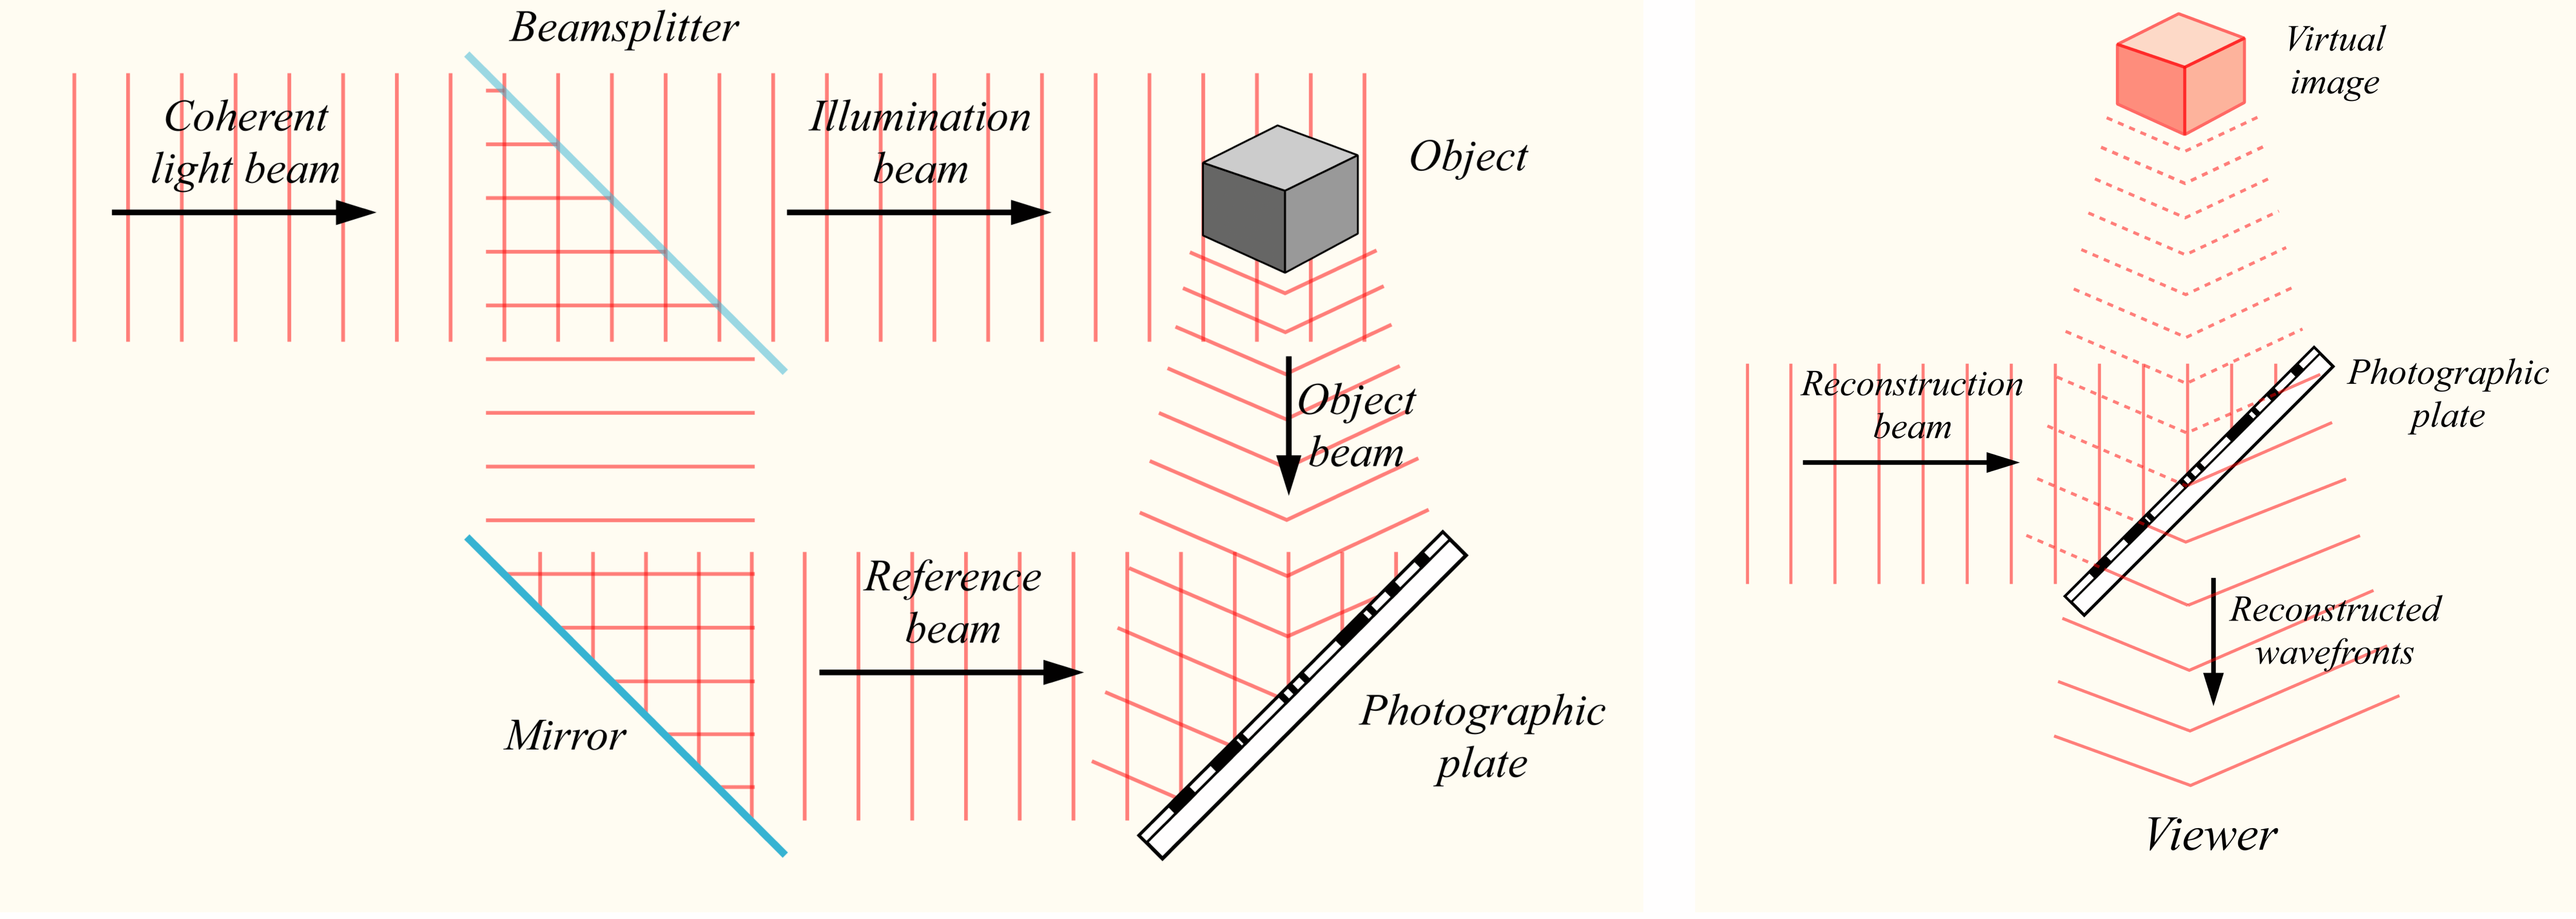
\includegraphics[width=1\linewidth]{./figs/holographySmall} 

}

\caption{Holografische opname en reconstructie. (Bron: Bob Mellish, Wikipedia)}\label{fig:hologram1}
\end{figure}

In de kwantummechanica hebben zowel materie als elektromagnetische golven\footnote{Voorbeelden van elektromagnetische golven zijn licht, microgolven en röntgenstraling} een deeltjes- en golfkarakter, en elke fysieke structuur wordt gedefinieerd door een golffunctie die zich in principe over het hele universum uitstrekt. \citet{bohm1980} wijst erop dat de kwantummechanica ons in staat stelt het universum en de werkelijkheid als één ononderbroken totaliteit, als één geheel, te begrijpen. Hij legt dit intuïtief uit in het volgende verhelderende voorbeeld: ``Als we naar de nachtelijke hemel kijken, kunnen we structuren onderscheiden die enorme uitgestrekte ruimte en tijd bestrijken, die in zekere zin vervat zijn in de bewegingen van het licht in de kleine ruimte die wordt omgeven door de oog en (\ldots) hoe instrumenten (\ldots) ook steeds meer van deze totaliteit kunnen onderscheiden, die is vervat in elk gebied van de ruimte.'' Dit heeft weer hoe volgens deze inzichten informatie over het hele universum, of over de totale orde ervan, impliciet wordt ``opgevouwen'' of vervat is in elk gebied van de ruimte-tijd, en hoe deze informatie terug kan worden ``ontvouwen'' door ons oog of door onze instrumenten. \citet{bohm1980} stelt verder dat deze ``opvouwing'' en ``ontvouwing'' niet alleen van toepassing is op lichtgolven, maar op elektromagnetische golven in het algemeen, en ook op andere golven zoals de elektronen-, protonen-, zwaartekracht-, geluidsgolven, \ldots{}

\citet{bohm1980} verving daarom de oude cartesiaanse analogie van het universum als machine door een nieuwe analogie: die van een holografisch universum, dat verwijst naar zijn ononderbroken en onverdeelde totaliteit die is ``opgevouwen'' in elk gebied van de ruimte-tijd.

Dus toen Rolando naar het universum verwees als een levend hologram, drukte hij zijn visie uit dat het leven deel uitmaakt van deze ononderbroken en onverdeelde totaliteit die is ``opgevouwen'' in elk gebied van de ruimte-tijd.

Om deze zienswijze beter te begrijpen, introduceren we Bohms voorbeeld van een zonnebloempit waaruit een hele plant groeit.

\emph{Timelapse van een groeiende zonnebloem (Source: \url{https://www.youtube.com/watch?v=_owPRdbaMdY})}

De plant is ook holografisch. Elk van zijn cellen bevat inderdaad alle informatie uit het zaad, dat wil zeggen al zijn DNA en zijn celstructuur. \citet{bohm1980} wijst er verder op dat het zaad weinig tot niets bevat van de volledige biomassa van de plant die eruit is gegroeid. Het zaad bevat slechts de informatie die nodig is om zijn omgeving te transformeren om de plant te laten groeien uit zonne-energie en de chaos van eenvoudige moleculen CO\(_2\), stikstof, fosfor, \ldots{} Opmerkelijk is dat de plant uiteindelijk nieuwe zaden zal produceren, die de informatie verder in de omgeving zullen verspreiden en deze steeds opnieuw zullen transformeren om planten te laten groeien. Het wordt dus duidelijk dat we niet langer een onderscheid hoeven te maken tussen ``levenloze'' en ``levende'' materie. Als we vasthouden aan deze oude cartesiaanse manier van denken, worden we geconfronteerd met verwarrende vragen zoals wanneer een zogenaamd ``levenloos'' koolstofatoom ``levend'' zou worden? Zodra het de bladhuidmondjes binnendringt of wanneer het wordt opgenomen in de suikers die in de bladgroenkorrels worden gevormd? Wordt het koolstofatoom weer ``levenloos'' als de plant de suikers die het heeft geassimileerd opnieuw tot CO\(_2\) verbrand tijdens de nacht? Al deze verwarrende vragen lossen spontaan op als we het universum als een ononderbroken en onverdeelde totaliteit bekijken. Vanuit dit paradigma gaan we ervan uit dat de omgeving wordt aangerijkt met de informatie van het zaad, dat op de een of andere manier zijn omgeving lijkt aan te sturen om de zonnebloem te laten groeien. Het leven zelf kan dus worden beschouwd als deel van het geheel dat de plant en zijn omgeving omvat. Het leven is op de een of andere manier in deze totaliteit ``opgevouwen'' en al impliciet aanwezig, nog voordat het zich ``ontvouwt'' en zich expliciet manifesteert. Alle atomen die uiteindelijk de zonnebloem zullen vormen die zal groeien uit het zaad, zijn immers al in de omgeving aanwezig. Het is de informatie in het zaad die de omgeving als het ware herstructureert om de plant te groeien. Op deze manier kan zogenaamde ``levenloze materie'' worden gezien als een subtotaliteit van het geheel waarin leven zich kan ontvouwen, bijvoorbeeld wanneer de omgeving wordt verrijkt met de informatie in een zonnebloempit. \citet{bohm1980} concludeert dus dat we het geheel niet hoeven op te splitsen in ``levende'' en ``levenloze'' materie, en dat we leven ook niet moeten proberen te reduceren tot iets dat volledig uit ``levensloze'' materie is voortgebracht.

Het zonnebloempitvoorbeeld is een prachtige illustratie van de synergie tussen anabasis en katabasis. Het proces van katabasis waarbij de zonnebloem sterft en desintegreert, draagt onmiddellijk de kiem in zich van nieuw leven dat verborgen ligt in de nieuwgevormde zaden. Zodra de zaden ontkiemen in een nieuwe omgeving begint het proces van anabasis of van de integratie en herstructurering van de omgeving immers opnieuw.

Het voorbeeld laat ook zien hoe relatief tijd is en hoe elk leven als een kosmische dans kan worden gezien. De dans van de zonnebloem duurde grofweg honderd dagen. Onze dans duurt ongeveer een eeuw. Uit het zonnebloempitvoorbeeld kunnen we dus leren dat we geduld moeten hebben met onze groei; het zal immers tijd kosten om onze sociale omgeving te transformeren. Het toont ook zo mooi aan dat we erop mogen vertrouwen dat alles al aanwezig is in onze omgeving. We hoeven alleen maar de tijd te nemen en de moed te hebben om onze omgeving te transformeren in de richting van onze groei.

Merk op dat het zonnebloempit-voorbeeld ook laat zien hoe krachtig het concept van een verrijkte omgeving is: wanneer we de omgeving verrijken met de informatie in het zonnebloemzaadje, wordt de omgeving als het ware aangestuurd om de prachtige zonnebloem te groeien. Deze analogie kan ook worden toegepast op onze menselijke wereld en was precies wat Rolando bedoelde met Biodanza: het bieden van een verrijkte omgeving die onze ontogenese kan beïnvloeden. Of hoe Biodanza de informatie of de ecofactoren creëert die onze omgeving verrijken om ons als mens te laten evolueren en dit zowel op fysiologisch als op psychogisch, sociaal en emotioneel vlak. Net als in het zonnebloempitvoorbeeld kunnen we daarna in onze eigen sociale omgeving gaan ontkiemen en deze met onze groei transformeren.

\hypertarget{het-universum-als-zelforganiserende-structuur}{%
\subsection{Het Universum als Zelforganiserende Structuur}\label{het-universum-als-zelforganiserende-structuur}}

Rolando noemde het universum ook de matrix van het leven, dat wil zeggen een zelforganiserende structuur die leven opbouwt en die op zichzelf moet worden begrepen als een gigantisch levend systeem.

Het universum zoals wij het kennen is waarschijnlijk begonnen met de oerknal: een enorme energiepiek. Kort na de oerknal ontstond er materie. Zoals \citet{davies1987} het beschrijft, was deze materie tamelijk vormloos en bestond die uit subatomaire deeltjes die min of meer uniform verdeeld waren in de ruimte bij een min of meer uniforme temperatuur. Paul Davies argumenteert verder dat het universum zich geleidelijk heeft ontwikkeld vanuit deze grotendeels vormloze toestand naar zijn huidige rijkdom aan fysische en chemische vormen en structuren. Of om hem te citeren: ``de creatieve kracht van de natuur manifesteerde zich vooral NA de eerste flits van het bestaan''. Het creatieve vermogen van de natuur blijft inderdaad doorheen alle tijden bestaan.

Ilya Prigogine was een van de eerste wetenschappers die de theorie ontwikkelde om uit te leggen hoe materie en energie het aangeboren vermogen hebben om zichzelf te organiseren. Convectiestromen zijn ondermeer een voorbeeld van een eenvoudig fysiek proces dat massieve structuren genereert. Ze kunnen worden waargenomen door een ondiepe laag vloeistof of gas van onderaf te verwarmen, waardoor een temperatuurgradiënt ontstaat die vloeistoffen in rusttoestand onstabiel maakt. De warmere vloeistof aan de onderkant is inderdaad lichter en begint naar boven te drijven waar hij weer afkoelt, terwijl de koudere vloeistof aan de bovenkant zwaarder is en naar de bodem zinkt, waar hij weer wordt verwarmd (zie Figuur \ref{fig:convectionCells}).

\begin{figure}

{\centering 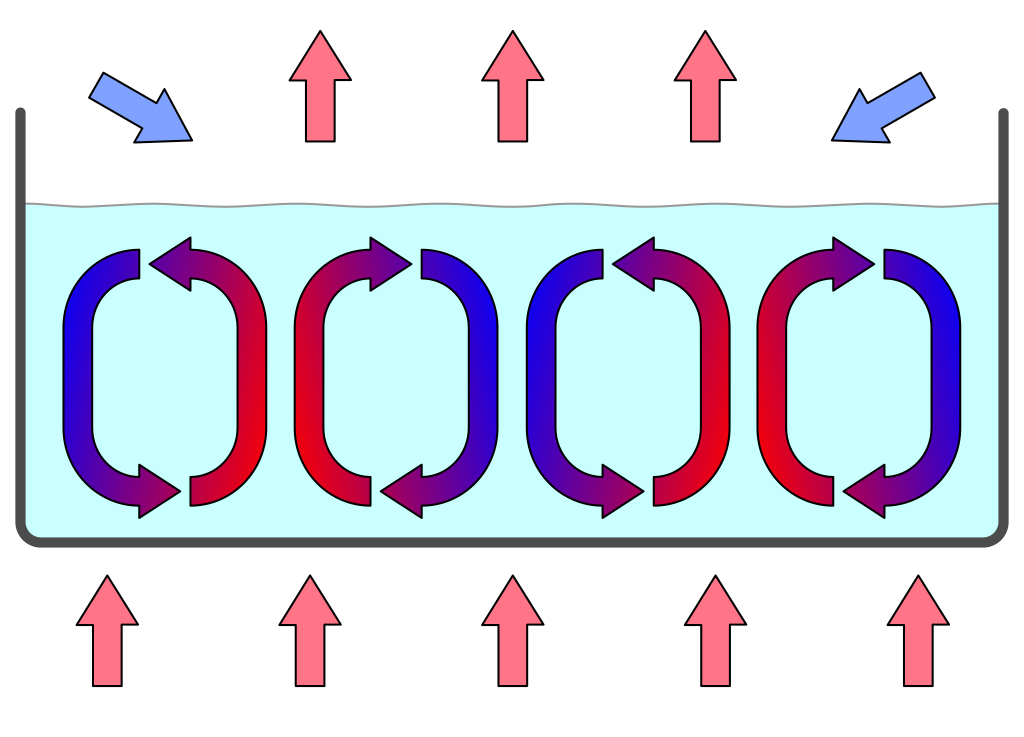
\includegraphics[width=0.8\linewidth]{./figs/convection_cells} 

}

\caption{Convectiecellen in een zwaartekrachtveld. Een vloeistoflaag wordt van onderaf verwarmd. De warmere vloeistof op de bodem wordt lichter en drijft naar boven waar hij weer afkoelt, terwijl de zwaardere, koudere vloeistof naar de bodem zinkt waar hij wordt verwarmd. Dit organiseert de vloeistoflaag in hexagonale convectiecellen (Bron: Wikipedia - users Eyrian and Con-struct)}\label{fig:convectionCells}
\end{figure}

De convectiebeweging leidt tot een spontane complexe ruimtelijke organisatie, bijna een dans, van miljarden moleculen die coherent bewegen en hexagonale convectiecellen vormen. Dergelijke convectiecellen kunnen worden waargenomen in een klein schaaltje met vloeistof in een laboratorium, tot op het niveau van de atmosfeer van de aarde en de fotosfeer van de zon (zie onderstaande filmpjes).

\emph{Bernard convectie cellen die ontstaan door olie op te warmen kunnen worden gevisualiseerd met grafiet (
\href{https://biodanzabrugge.be/biologischeAspectenBiodanza/figs/BernardCellenIk.mp4}{link video clip})}

\emph{De zonnefotosfeer waargenomen met de Zweedse 1-m Solar Telescope (SST) op La Palma, Spanje. De film toont zonnegranulatie die het resultaat is van convectieve bewegingen van bellen heet gas die uit het binnenste van de zon opstijgen. Wanneer deze bellen het oppervlak bereiken, koelt het gas af en stroomt het weer naar beneden in de donkerdere banen tussen de heldere cellen. In deze zogenaamde intergranulaire stroken kunnen we ook kleine heldere punten en meer uitgebreide heldere langwerpige structuren zien. Dit zijn gebieden met sterke magnetische velden. (Bron: Wikipedia, gebruiker Luc.rouppe, link: \url{https://en.wikipedia.org/wiki/File:Granulation_Quiet_Sun_SST_25May2017.webm})}

Prigogine toonde aan dat spontane zelforganisatie ook voorkomt in chemische systemen die zich ver van hun evenwichtstoestand bevinden doordat er voortdurend materie en energie doorheen wordt gestuwd. Deze zelforganiserende processen zijn grotendeels onvoorspelbaar en ontstaan spontaan in ons universum. \citet{prigogineStengers1984} argumenteren verder dat dergelijke chemische en fysische processen de basis vormen van de complexe zelforganisatie die we waarnemen in biologische systemen.

Dus in plaats van vast te houden aan de destructieve scheiding tussen mens en natuur, of aan het even destructieve idee dat wij mensen maar een incidenteel en irrelevant onderdeel van de kosmos zijn, kunnen we onszelf beter omarmen als kinderen van het universum. Een resultaat van zijn opmerkelijke creativiteit en met een schoonheid die lijkt op alle prachtige zelforganiserende structuren die ons omringen.

\hypertarget{organisatie-van-dit-hoofdstuk}{%
\subsection{Organisatie van dit hoofdstuk}\label{organisatie-van-dit-hoofdstuk}}

Dit hoofdstuk bouwt voort op het werk van vijf invloedrijke en wiens inzichten ons kunnen helpen om de biologische aspecten die Rolando Toro in zijn Biodanza Model heeft ingebed beter te begrijpen:

\begin{itemize}
\item
  Erwin Schrödinger die het leven expliciet definieerde als het structureren van ``orde-uit-wanorde'' en Ilia Prigogine die hiervoor de theorie ontwikkelde en de term ``Dissipatieve Structuren'' bedacht,
\item
  Christian de Duve, één van de grondleggers van de biochemie, en
\item
  Humberto Maturana en Francisco Varela met hun concept van autopoiese.
\end{itemize}

Merk op dat de subsecties in ``Christian de Duve: een Biochemische Visie op het Leven'' altijd beginnen met een algemeen overzicht, gevolgd door subsecties met meer technische details. Ik heb ervoor gekozen om deze technische details in deze monografie op te nemen, omdat ze geïnteresseerde lezers kunnen helpen alle termen en concepten te begrijpen die slechts heel kort aan bod komen in de reader van de Biodanza lerarenopleiding ``Module IV: Biologische Principes van Biodanza''. De secties ``Maturana en Varela: een Systeemvisie op het Leven'' en ``Links met Vitaal Onbewuste'' zijn meer filosofisch van aard.

\newpage

\hypertarget{schruxf6dinger-en-prigogine-een-thermodynamische-visie-op-het-leven}{%
\section{Schrödinger en Prigogine: een Thermodynamische Visie op het Leven}\label{schruxf6dinger-en-prigogine-een-thermodynamische-visie-op-het-leven}}

In zijn baanbrekende lezingenreeks: ``What Is Life? The Physical Aspect of the Living Cell'' definieerde '' \citet{schrodinger1944} leven als

\begin{enumerate}
\def\labelenumi{\arabic{enumi}.}
\item
  een open systeem dat orde kan scheppen in de chaos door externe energiebronnen te exploiteren,
\item
  met het vermogen om zijn eigen specifieke blauwdruk van generatie op generatie over te dragen.
\end{enumerate}

Merk op dat \citet{schrodinger1944} in zijn reeks lezingen ook de sleutelfuncties beschreef van de molecule die betrokken is bij deze blauwdruk en dat terwijl DNA nog niet was ontdekt.

In eerste instantie lijkt de eigenschap dat het leven orde of structuur kan genereren in tegenspraak met de tweede wet van de thermodynamica, die stelt dat een systeem altijd streeft naar maximale entropie.

Entropie kan losjes worden gedefinieerd als een fysieke grootheid die weergeeft hoe uitgespreid energie is. Het is dus de neiging van een systeem om te evolueren van een geconcentreerde energietoestand naar een energietoestand die meer verspreid is. Dit kan gemakkelijk worden begrepen aan de hand van een eenvoudig voorbeeld dat ieder van ons kent: als je een hete pot in een grote kamer zet, zal de pot afkoelen en zal de temperatuur in de kamer iets stijgen totdat de pot en de kamer dezelfde temperatuur hebben. Hierdoor wordt de geconcentreerde warmte-energie uit de pot mooi verspreid over de gehele ruimte. Dus de toename van de entropie is de natuurkundige analogie van katabasis.

Schrödinger begreep dat het leven deze tweede wet niet schendt. Doordat het een \emph{open} systeem is, kan het interageren met de omgeving, en door te eten en te ademen moet er een manier zijn om `de orde te concentreren' of een hogere, meer geconcentreerde energietoestand te handhaven.

Prigogine ontwikkelde het theoretische kader voor een type chemie dat essentieel is voor het leven \citep{prigogineStengers1984}. Hij realiseerde zich dat de chemie van het leven totaal anders is dan de meeste chemische systemen die tot dan toe werden bestudeerd. De chemie en de processen van het leven zijn inderdaad zeer niet-lineair met veel terugkoppelingslussen of feedbacklussen\footnote{Er ontstaat een feedbacklus in een chemisch systeem als een deel van de geproduceerde moleculen, de output opnieuw als input wordt gebruikt.}. Deze chemie bevindt zich ver van een evenwichtstoestand doordat er voortdurend materie en energie doorheen het systeem wordt gestuurd.

Dit laatste weten we intuïtief: ons lichaam bevindt zich doorgaans in een hogere energietoestand dan het overeenkomstige materiaal in een ``niet-levende'' staat. We kunnen dat eenvoudigweg erkennen, omdat we meestal warmer zijn dan de kamer waarin we ons bevinden, en een ruwe manier om in te schatten hoe lang iemand dood is, is door de temperatuur van het lijk te meten. Om onze hogere energietoestand te behouden, om chemische stoffen in onze cellen te concentreren en om daaruit complexe moleculen, cellen en weefsels op te bouwen, moeten we blijven eten en ademen.

\pagebreak

\hypertarget{dissipatieve-structuren}{%
\subsection{Dissipatieve Structuren}\label{dissipatieve-structuren}}

Prigogine ontdekte dat complexe zelforganiserende systemen spontaan kunnen ontstaan als ze open zijn en veel energie en materie kunnen uitwisselen met hun omgeving. Essentieel voor deze ``anabasis'' is een chaos van materie en een stroom van energie door het systeem. In chemische systemen, en het leven is voor een groot deel chemie, maakt de instroom van energie het mogelijk om structuur te genereren, terwijl er door dissipatie veel entropie wordt geproduceerd. Dissipatie betekent dat energie van een meer geconcentreerde energievorm naar een minder geconcentreerde energievorm is omgezet. Dissipatie is dus onomkeerbaar, wat de pijl van de tijd aan het leven toevoegt. De omzetting van energie in warmte vindt plaats in de meeste onderliggende biochemische reacties. Deze kunnen dus niet worden omgekeerd zonder de toevoeging van nieuwe energie. Daarom wordt een groot deel van de geconcentreerde energie die de cellen binnendringt via zonlicht of chemische energie onder de vorm van voedsel, verspreid in een minder geconcentreerde energievorm: warmte.

De structuur die spontaan ontstaat in levende organismen schendt dus de tweede wet niet omdat ze gepaard gaat met de stijging van de entropie door de afvoer van warmte. Dat laat opnieuw zien hoe de processen van anabasis en katabasis hand in hand gaan. Prigogine bedacht daarom de nieuwe term ``dissipatieve structuren'' voor dergelijke systemen.

\hypertarget{attractoren}{%
\subsection{Attractoren}\label{attractoren}}

In de reader van de Biodanza lerarenopleiding ``Module II Vitaal Onbewuste en Biocentrisch Principe'' gebruikt Rolando Toro vaak de term ``attractor''. Dissipatieve structuren hebben doorgaans meerdere attractoren, dat wil zeggen staten, regimes, vormen of structuren waarnaar ze spontaan evolueren. De specifieke attractor waarrond het systeem zichzelf organiseert, hangt sterk af van de initiële omgevingsomstandigheden. Merk op dat dissipatieve structuren ook worden gekenmerkt door feedbacklussen. Deze feedbacklussen zorgen voor een soort homeostase zodat het systeem bij veranderingen in de omgeving, bij zijn huidige attractor kan blijven. Sommige omgevingsstimuli worden echter versterkt door de feedbacklussen en kunnen de dissipatieve structuur van attractor laten wisselen en zo een regimewisseling teweegbrengen.

Prigogine argumenteerde dat de chemie in cellen, de cellen zelf, weefsels, organen, organismen, populaties van organismen, ecosystemen en onze gehele aarde kunnen worden gezien als dissipatieve structuren \citep{prigogineStengers1984}.
Slijmzwammen zijn een voorbeeld van een levend systeem dat vaak verandert van attractor, zie Figuur \ref{fig:Dictyostelium}. Dictyostelium-slijmzwammen brengen het grootste deel van hun leven door als afzonderlijke eencellige amoebes. Maar bij stress geeft één van de amoeben een biochemische signaalmolecule cAMP af. Anderen detecteren dat signaal en reageren op twee manieren: de amoebe beweegt naar het signaal toe en scheidt zelf ook cAMP af, waardoor het signaal effectief wordt versterkt. Het signaal triggert dus een feedbacklus die er uiteindelijk voor zorgt dat het systeem overschakelt van hun huidige attractor -- een toestand van vrijlevende amoeben -- naar een nieuwe attractor -- het vruchtlichaam -- die sporen vrijgeeft en de slijmzwammen naar nieuwe omgevingen zal verspreiden (zie bijvoorbeeld youtube clip \url{https://youtu.be/bkVhLJLG7ug}).

\pagebreak

\begin{figure}

{\centering 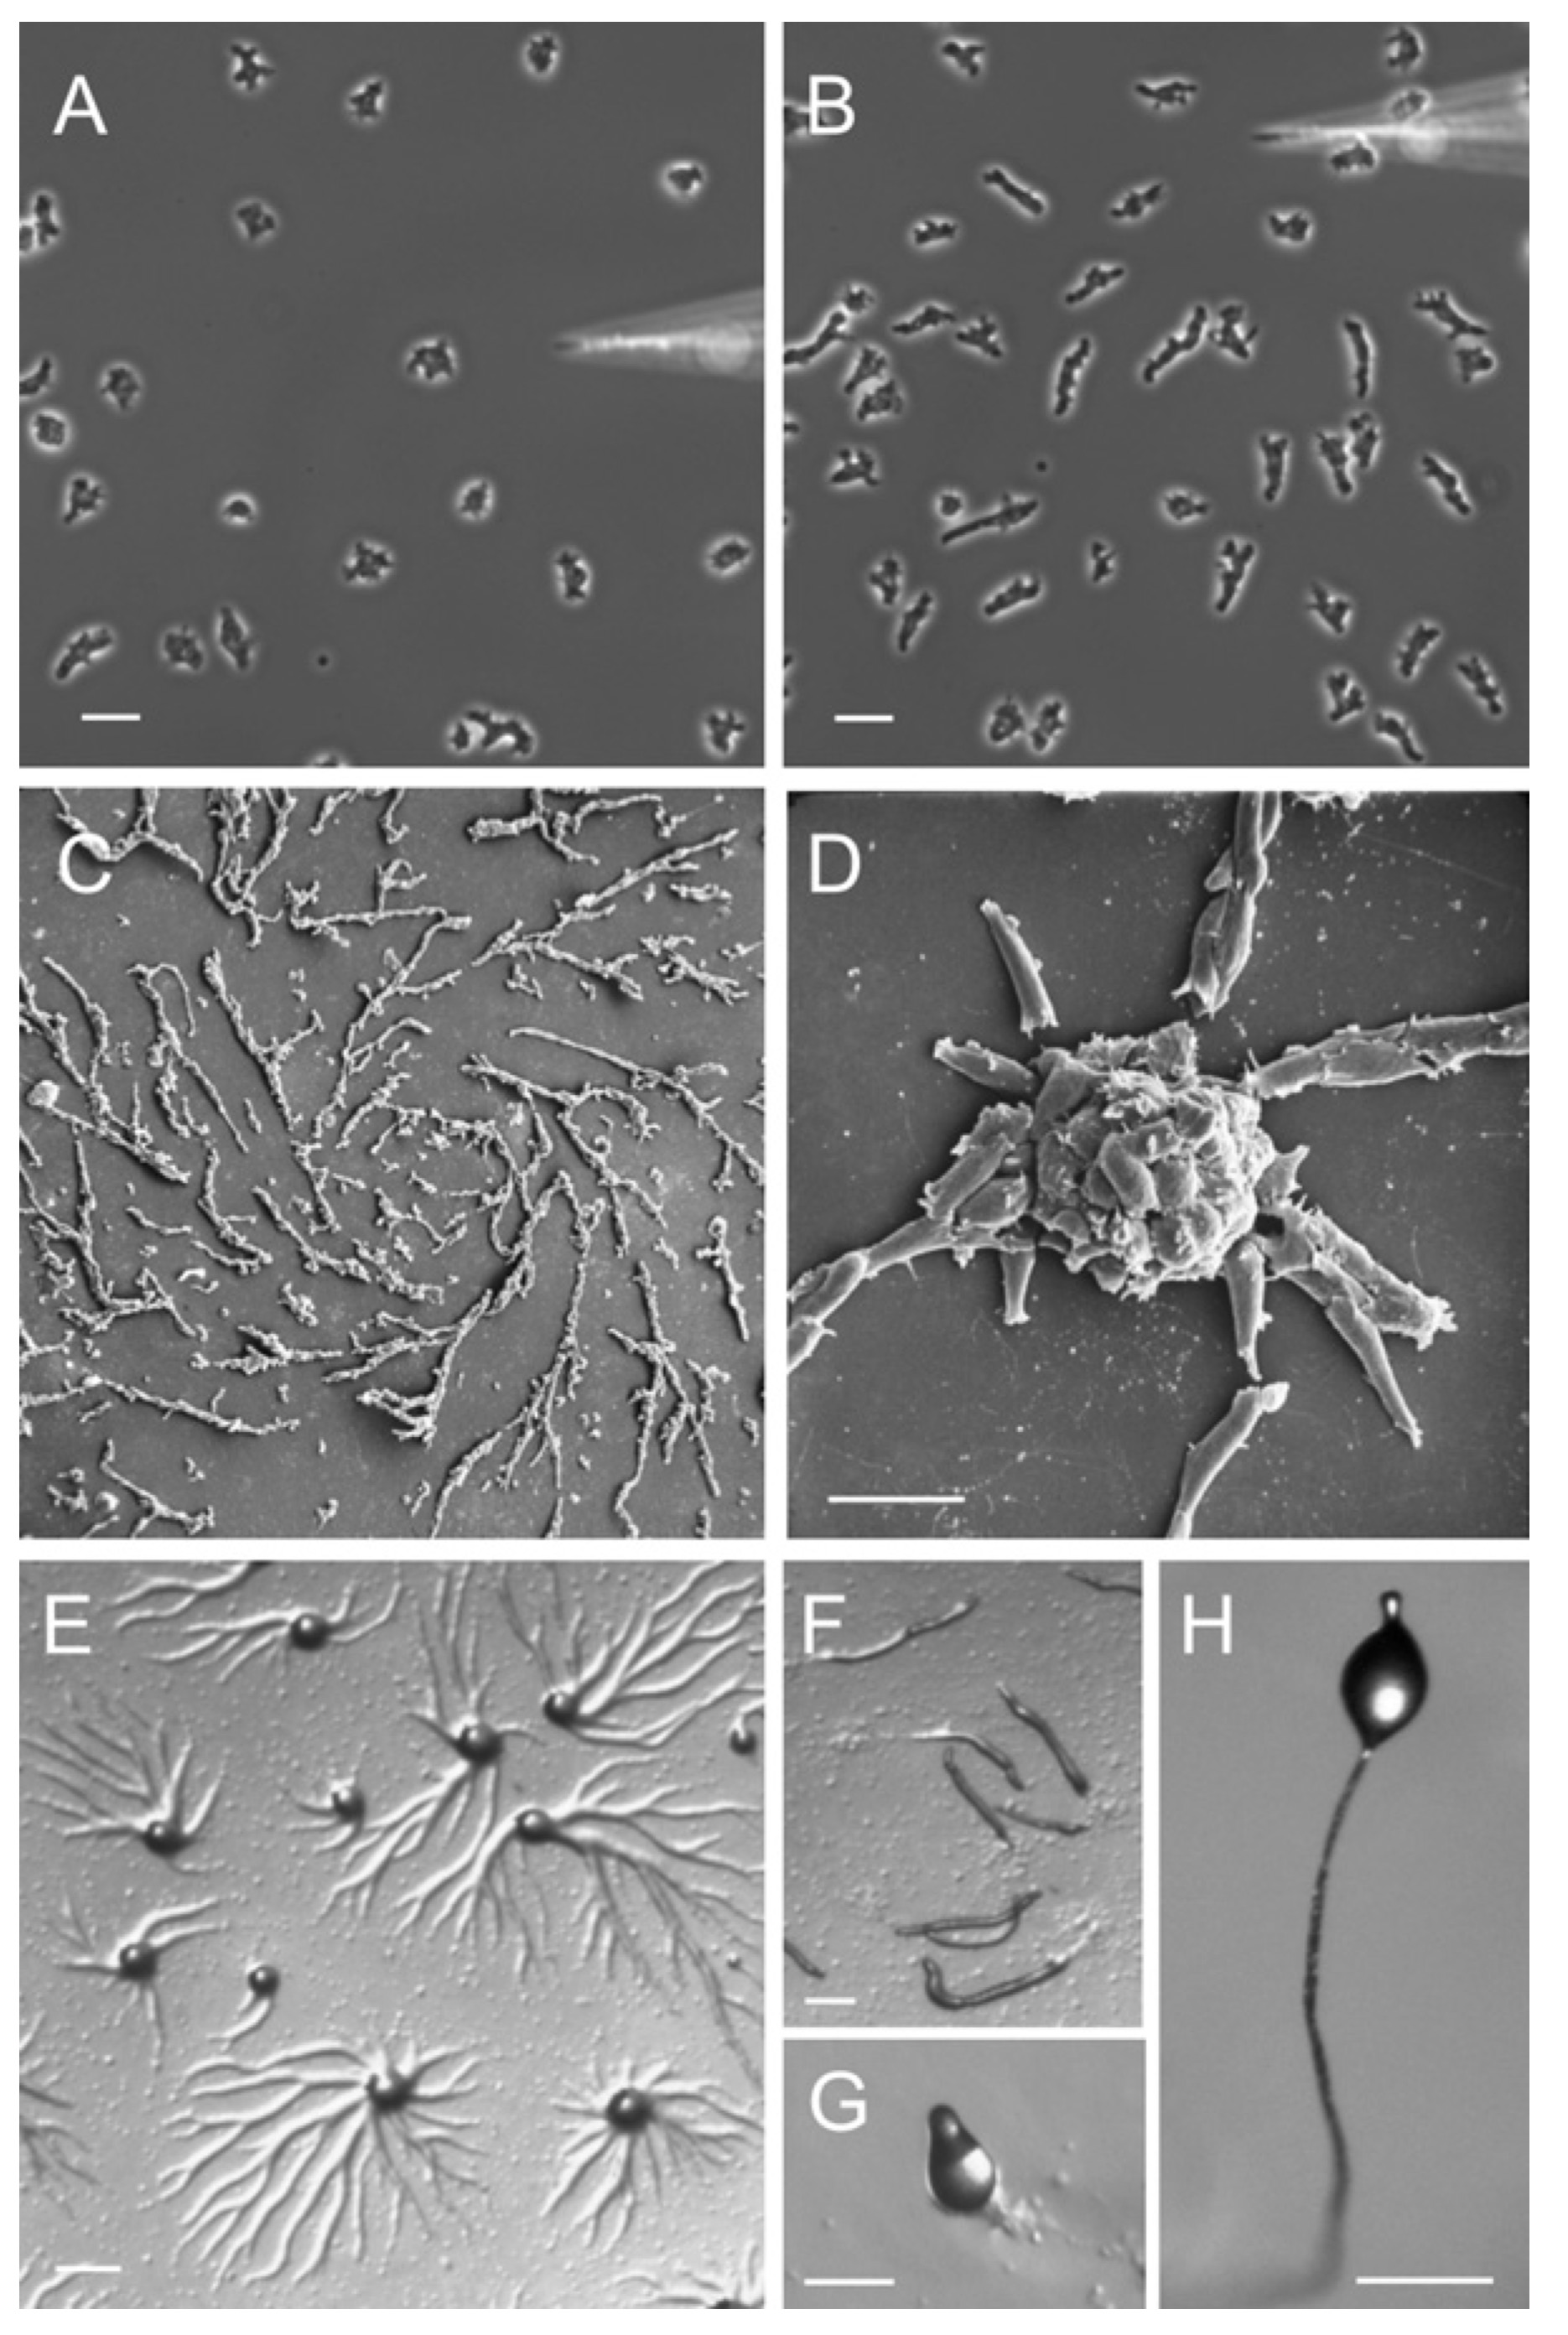
\includegraphics[width=0.6\linewidth]{./figs/Dictyostelida} 

}

\caption{Stadia van de levenscyclus van Dictyostelium. (A - B) Dictyosteliumcellen bewegen naar cAMP dat wordt toegediend met een micropipet. Cellen die cAMP nog niet hebben waargenomen, worden getoond in (A). Binnen 1 of 2 minuten polariseren de cellen en migreren ze naar de cAMP bron (B). (C - D) Rasterelektronenmicrofoto van stromende Dictyostelium-cellen (C) en de vorming van aggregaten (D). (E) Vorming van aggregatiecentra op een agarplaat. (F) De aggregaten bewegen op een agarplaat. (G) Culminatiefase. (H) Vruchtlichaam. Figuur van Müller-Taubergen et al. 2012}\label{fig:Dictyostelium}
\end{figure}

Het Dictyostelium-voorbeeld laat ook duidelijk dat instincten heel precies zijn en hoe ze diep verankerd zijn in de biochemie van het leven. We kunnen in het voorbeeld de instincten herkennen van

\begin{itemize}
\tightlist
\item
  exploratiegedrag bij vrijlevende amoeben
\item
  tropisme/chemotaxis wanneer alle amoeben zich omdraaien en in de richting van het cAMP-signaal beginnen te bewegen
\item
  behoud, solidariteit en seksualiteit wanneer zij zich organiseren in een vruchtlichaam.
\end{itemize}

Deze instincten worden gedeeld door alle levensvormen, maar hun expressie is gedifferentieerd bij verschillende soorten. Instincten zijn dus de attractoren van het leven. Daarom was de bevrijding van onze instincten zo belangrijk voor Rolando Toro. Met Biodanza zullen we ons opnieuw met onze instincten verbinden en ze versterken langs de vijf lijnen van Biodanza, die elk verbonden zijn met deze overkoepelende instincten.

Het instinct van behoud is bijvoorbeeld verbonden met de lijn van vitaliteit, seksualiteit met de lijn van seksualiteit, exploratiegedrag met de lijn van creativiteit, solidariteit met de lijn van affectiviteit, en tropisme met de lijn van transcendentie\footnote{Merk op dat we alleen de instincten hebben opgenomen die te zien zijn in het Dictyostelium-voorbeeld. Er zijn dus meer overkoepelende instincten gekoppeld aan deze vijf lijnen die je terug kan vinden in het boek van Rolando over Biodanza \citep{toro2008}.}.

\hypertarget{dissipatieve-zones}{%
\subsection{Dissipatieve zones}\label{dissipatieve-zones}}

In de reader van de Biodanza lerarenopleiding ``Module II Vitaal Onbewuste en Biocentrisch Principe'' wordt ook vermeld dat we in een dissipatieve zone leven. De gehele aarde kan worden gezien als een grote dissipatieve structuur in ons zonnestelsel, wat een dissipatieve zone is.

\begin{enumerate}
\def\labelenumi{\arabic{enumi}.}
\item
  De zon is een energiebron die geconcentreerde energie onder de vorm van fotonen uitstraalt.
\item
  Cyanobacteria en planten organiseren structuur uit de chaos van moleculen op aarde door energie van de fotonen van de zon, licht en UV, te dissiperen naar warmte via hun organische pigmenten, zoals chlorofyl.
\item
  Dieren, bacteriën en schimmels zijn secundaire dissipatieve structuren die zich voeden met de geconcentreerde chemische energie in de vorm van suiker, zetmeel, eiwitten en vetten die worden geproduceerd door planten en cyanobacteriën. Ze dissiperen opnieuw energie in de vorm van warmte door hun celademhaling.
\item
  De warmte die door het biologische leven wordt geproduceerd wordt afgevoerd naar water en lucht en dit veroorzaakt tertiaire dissipatieve processen zoals de watercyclus, wind- en zeestromingen, \ldots{}
\item
  Uiteindelijk wordt warmte naar de ruimte uitgestraald.
\end{enumerate}

Omdat de temperatuur op aarde ongeveer stabiel blijft, wordt er ongeveer evenveel energie in de vorm van warmte naar de ruimte uitgestraald als wat binnenkomt onder de vorm van fotonen van de zon. Omdat de energie-inhoud van warmte lager en meer verspreid is, heeft deze een hogere entropie dan die van het binnenkomend zonlicht. Omdat er bijna geen materie wordt uitgewisseld tussen de aarde en de ruimte, moet materie worden gerecycleerd en is het leven inherent cyclisch.

Deze cyclische aard van het biologische leven met zijn eeuwige terugkeer is de sleutel tot vernieuwing en vitaliteit. Dat wordt in alle menselijke culturen erkend zoals blijkt uit hun rijke rituelen die deze cyclische oorsprong vieren. Maar ze zijn door ons westerse denken echter in onbruik geraakt.

Biodanza erkent het belang van verbinding en resonantie met onze cyclische oorsprong. Biologische regressie in Biodanza is inderdaad een moment van terugkeer naar en verbinding met onze oorsprong. Dat initieert en versterkt vernieuwingsprocessen, zowel op biologisch, fysiologisch als op psychologisch, sociaal en emotioneel vlak.

\newpage

\hypertarget{de-duve-een-biochemische-visie-op-het-leven}{%
\section{de Duve: een Biochemische Visie op het Leven}\label{de-duve-een-biochemische-visie-op-het-leven}}

In zijn boek ``Life Evolving - Molecules, Mind and Meaning'', gaf \citet{deDuve2002} een heel eenvoudige maar briliante definitie van leven:

Leven is

\begin{enumerate}
\def\labelenumi{\arabic{enumi}.}
\tightlist
\item
  Één,
\item
  Chemie, en
\item
  Informatie
\end{enumerate}

In de volgende secties staan we stil bij wat De Duve bedoelde met elk onderdeel van zijn definitie. Merk op dat elke sectie begint met het kernidee en vervolgens bestaat uit meer technische subsecties die de biologische concepten in de reader ``Module IV Biologische aspecten van Biodanza'' in meer detail introduceren.

\hypertarget{lifeOne}{%
\subsection{Leven is Één}\label{lifeOne}}

Het eerste deel van de definitie van De Duve, ``Het leven is één'', was heel belangrijk voor Rolando Toro toen hij de term ``Vitaal onbewuste'' bedacht.

``Het leven is één'' omdat alle levende organismen op aarde

\begin{itemize}
\tightlist
\item
  zijn opgebouwd uit cellen
\item
  geëvolueerd zijn uit dezelfde soort, LUCA, onze laatste universele gemeenschappelijke voorouder
\item
  dezelfde molecule gebruiken voor het opslaan, omzetten en gebruiken van energie
\item
  zijn opgebouwd uit dezelfde biologische bouwstenen: lipiden, suikers, aminozuren voor eiwitten en nucleïnezuren (DNA en RNA).
\end{itemize}

\hypertarget{alle-levende-organismen-zijn-opgebouwd-uit-cellen}{%
\subsubsection{Alle Levende Organismen Zijn Opgebouwd uit Cellen}\label{alle-levende-organismen-zijn-opgebouwd-uit-cellen}}

``Het leven is één'' omdat alle organismen uit cellen bestaan. Groene algen die fotosynthese kunnen uitvoeren zijn een mooi voorbeeld van eencellige organismen. Ze waren van cruciaal belang voor de ontwikkeling van het leven op onze planeet doordat ze zuurstof produceren die een belangrijke component is van onze atmosfeer (Figuur \ref{fig:greenAlgae}).

\begin{figure}

{\centering 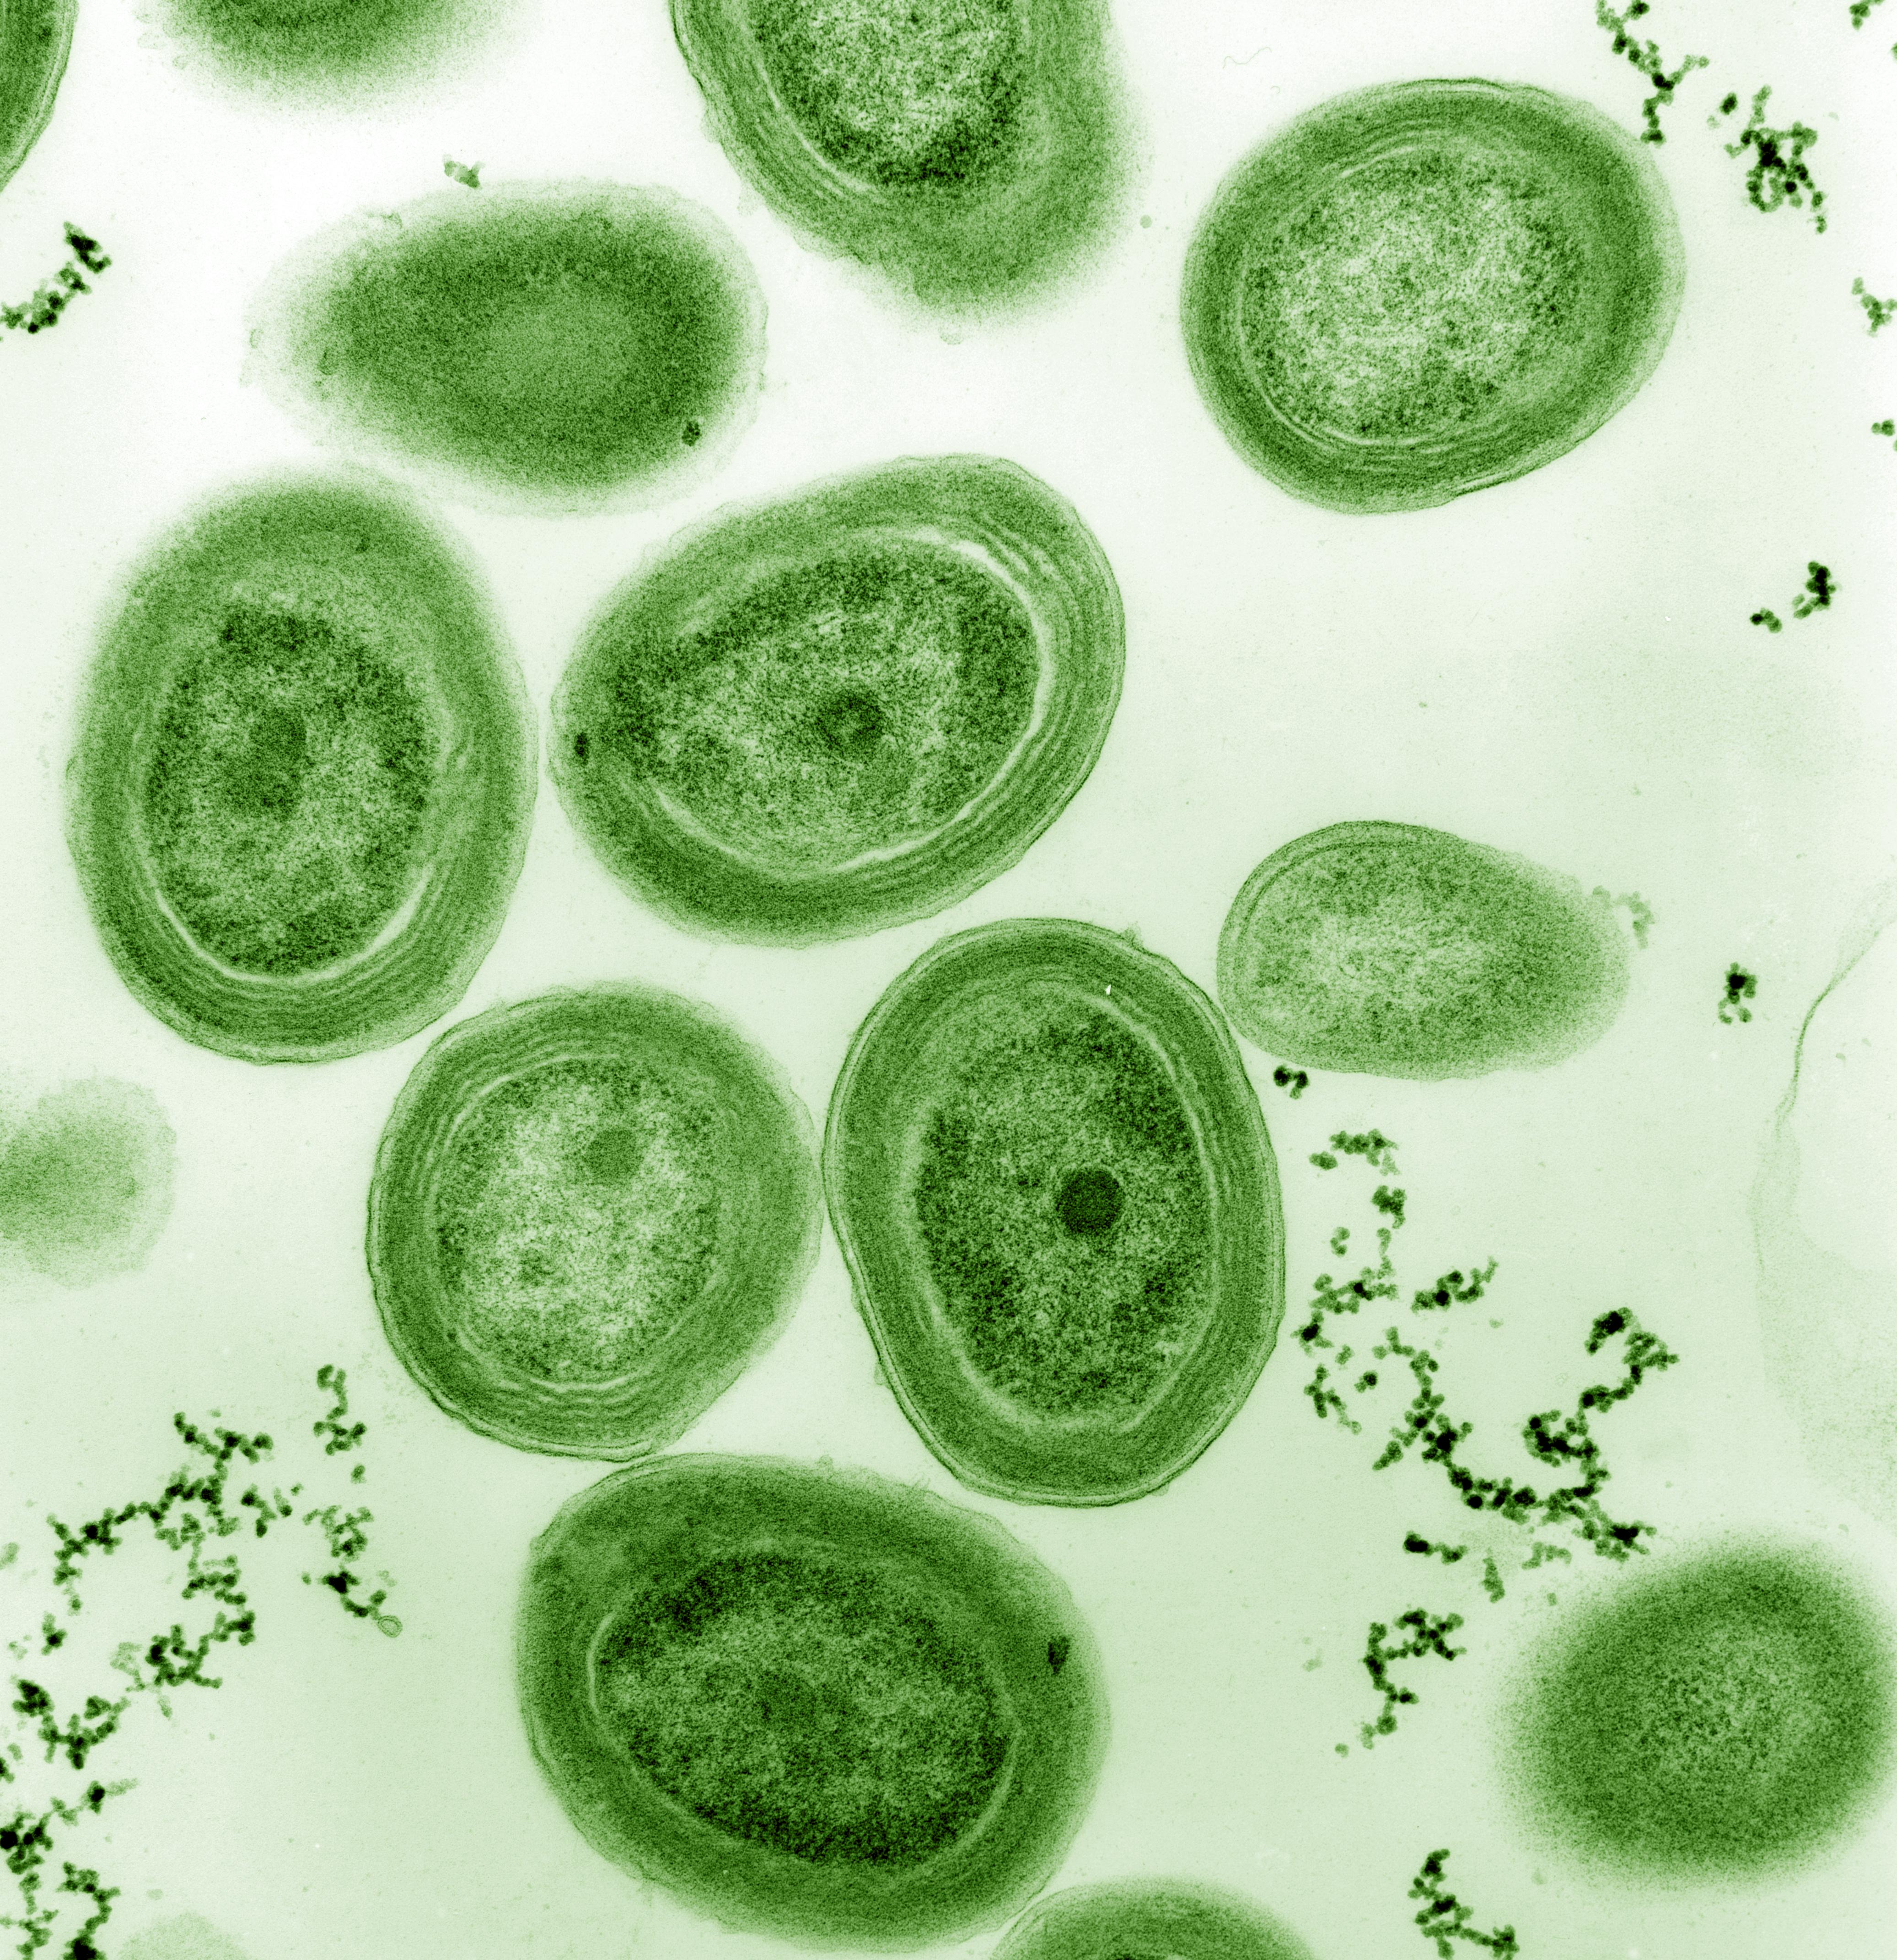
\includegraphics[width=0.3\linewidth]{./figs/Prochlorococcus_marinus} 

}

\caption{Cyanobacteriën, eencellige organismen die aan fotosynthese doen. Ze speelden een sleutelrol in de ontwikkeling van het leven en veranderden de aarde radicaal door zuurstof in onze atmosfeer te brengen (Bron: Chisholm Lab, Wikipedia)}\label{fig:greenAlgae}
\end{figure}

Een essentieel onderdeel van een cel is het membraan (de buitenste laag van de cel) dat hen scheidt van hun omgeving, terwijl het ze toch toelaat om ermee te interageren en chemicaliën in de cel te concentreren.

Meercellige organismen bestaan uit meerdere cellen. De cellen zijn georganiseerd in weefsels, bijvoorbeeld sponsachtig weefsel in onze botten of epitheelcellen van onze maag. Weefsels zijn georganiseerd in organen, b.v. botten of onze maag. Organen zijn georganiseerd in orgaansystemen, b.v. skelet of spijsverteringsstelsel. Orgaansystemen vormen een organisme. Figuur \ref{fig:multiCellular} laat ook zien hoe organismen verder georganiseerd zijn in populaties van organismen, ecosystemen en uiteindelijk onze hele biosfeer. Dus het ``leven is één'' omdat alle levende organismen bestaan uit cellen die georganiseerd zijn in grote netwerken die samenwerken.

\begin{figure}

{\centering 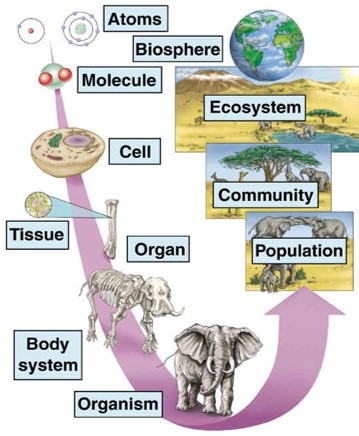
\includegraphics[width=0.3\linewidth]{./figs/organisationMulticellular} 

}

\caption{Multicellulaire organismen en biologische organisatie (Bron: mrssmithsbiology)}\label{fig:multiCellular}
\end{figure}

\pagebreak

\hypertarget{laatste-universe-gemene-voorouder}{%
\subsubsection{Laatste Universe Gemene Voorouder}\label{laatste-universe-gemene-voorouder}}

``Het leven is één'' omdat alle soorten zijn geëvolueerd uit dezelfde voorouderlijke populatie van cellen. Dit wordt ook wel de Last Universal Common Ancestor (LUCA) genoemd. Dit wordt mooi aangegeven door de levensboom in Figuur \ref{fig:treeOfLife}, één van de meest belangrijke organisatieprincipes in de biologie. Het toont de evolutionaire relaties tussen verschillende organismen en dat alle levende wezens uiteindelijk terug te voeren zijn op LUCA, die zich aan de wortel van de boom bevindt. Merk op dat het dierenrijk waartoe wij behoren slechts een kleine zijtak is van de boom.

\begin{figure}

{\centering 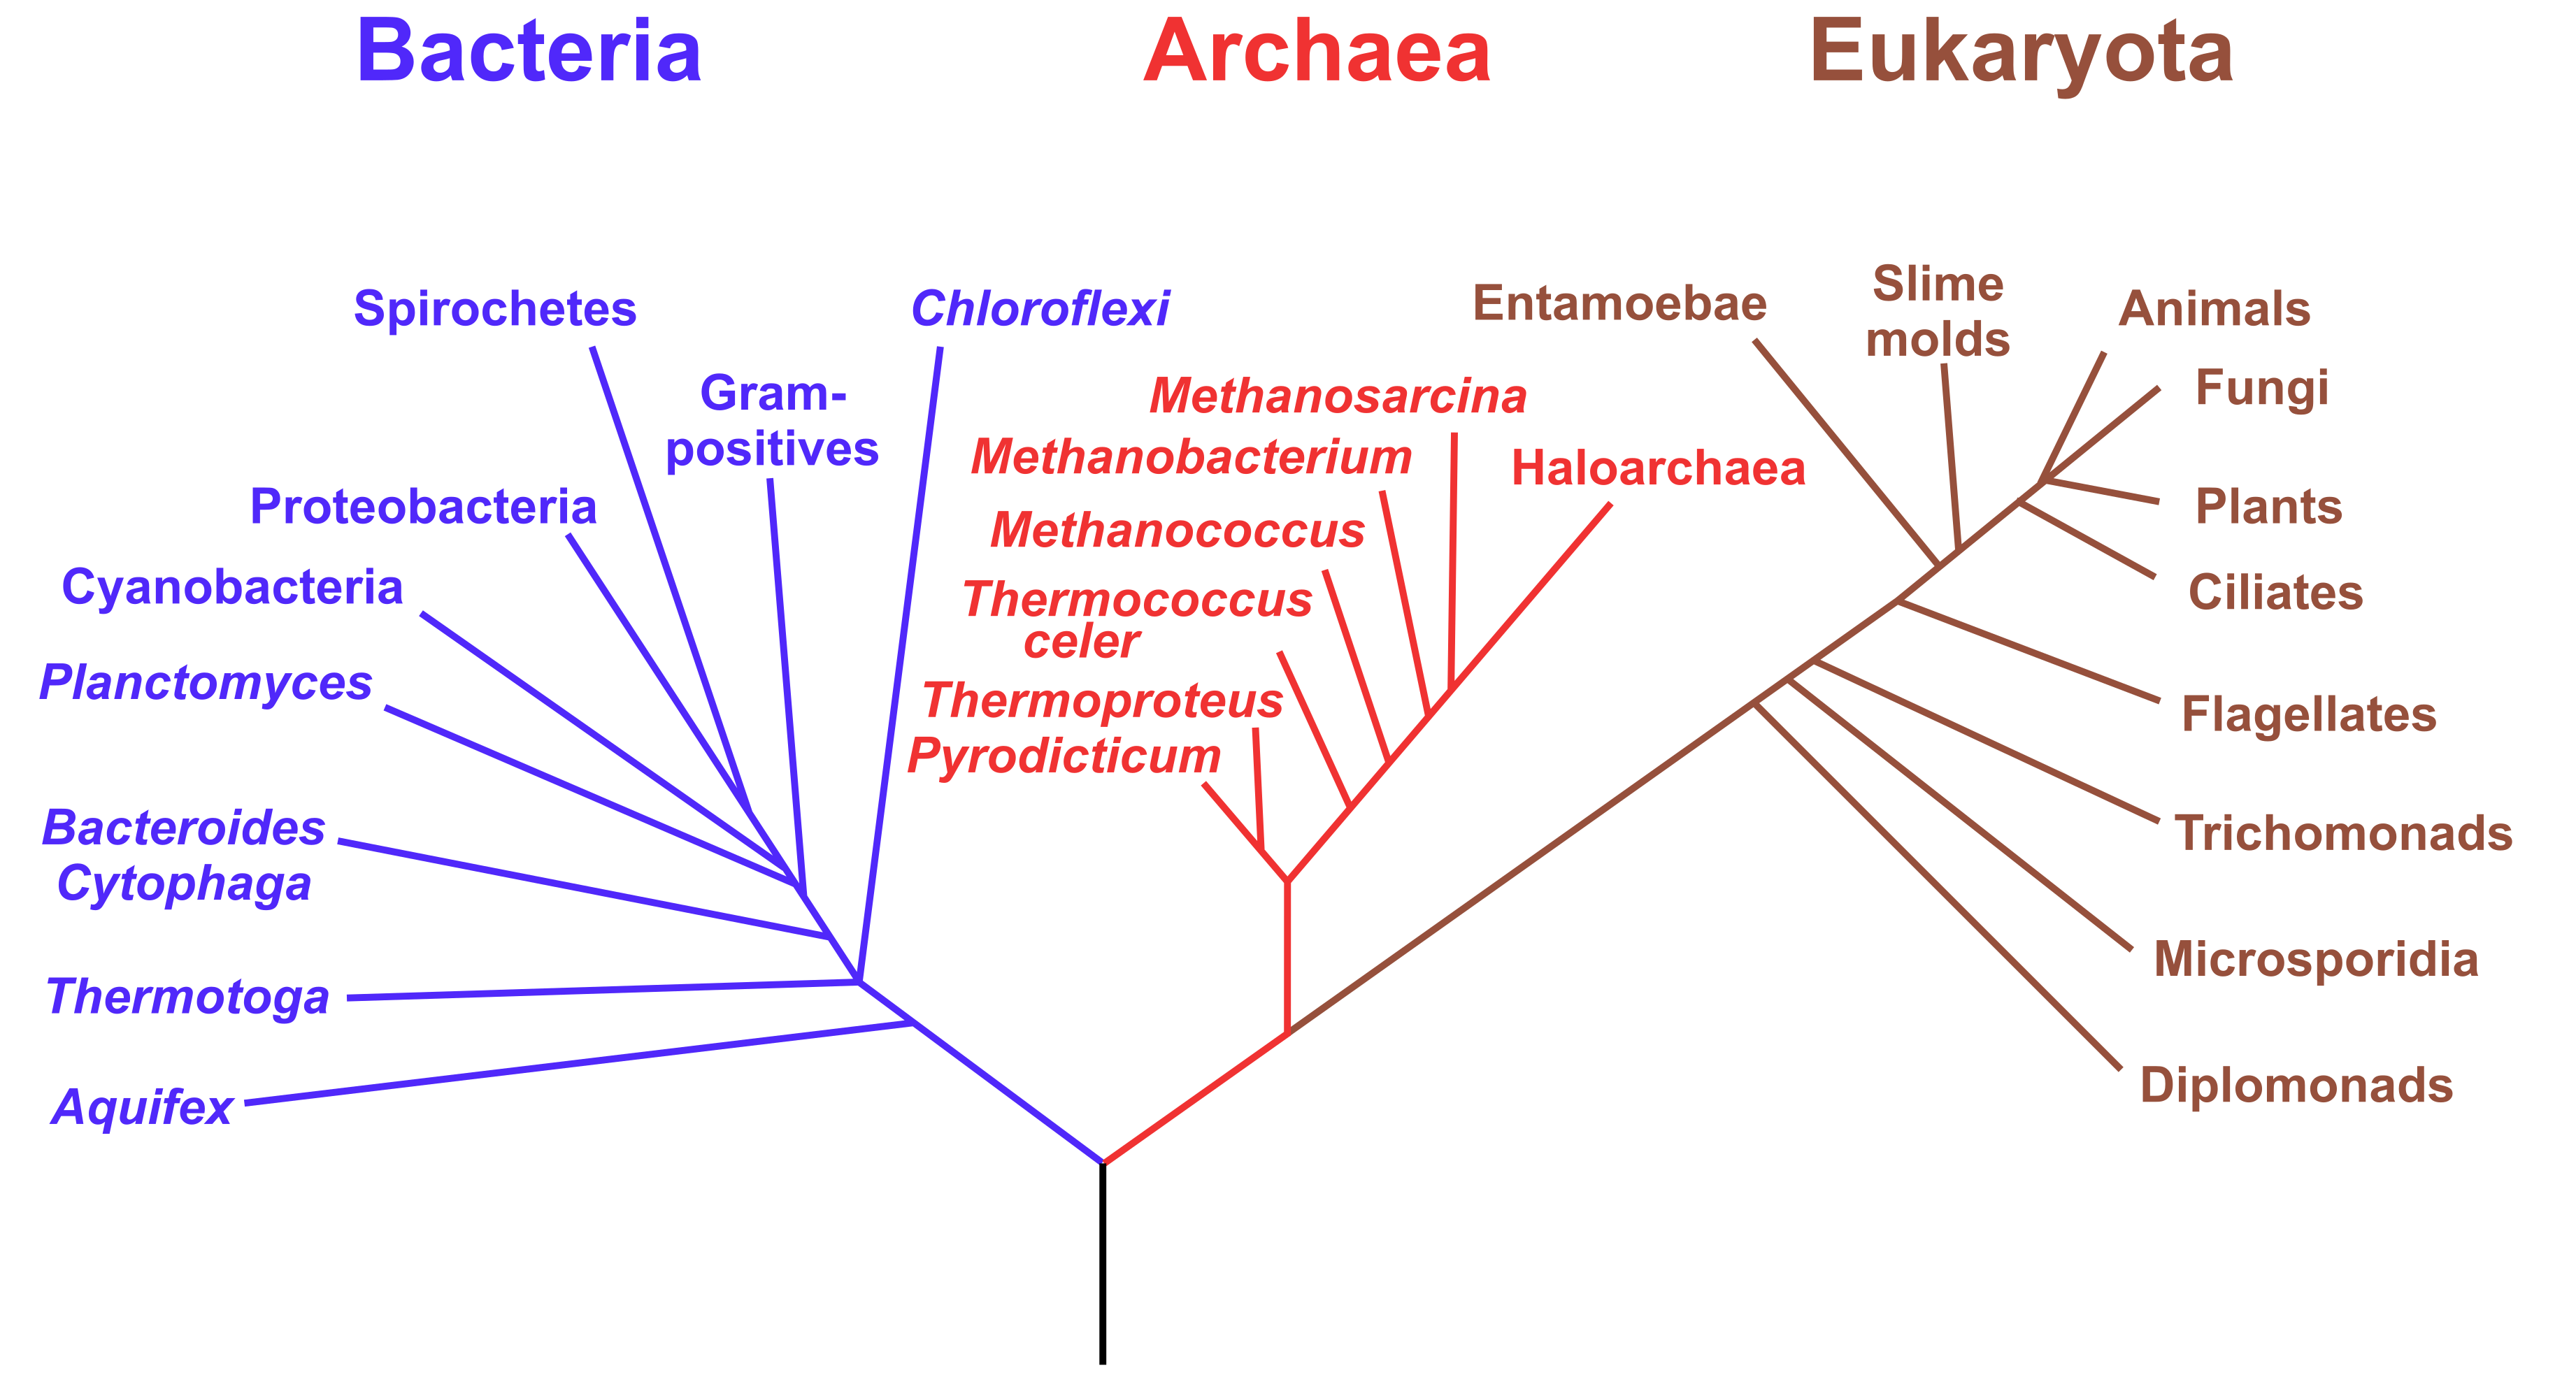
\includegraphics[width=0.8\linewidth]{./figs/Phylogenetic_tree} 

}

\caption{De levensboom is één van de meest belangrijke organisatieprincipes in de biologie. Het toont de evolutionaire relaties tussen verschillende organismen en ook dat alle levende wezens uiteindelijk terug te voeren zijn op de laatste universele gemeenschappelijke voorouder (LUCA), die zich aan de wortel van de boom bevindt (Bron: Wikipedia)}\label{fig:treeOfLife}
\end{figure}

\hypertarget{sectionEnergyCoin}{%
\subsubsection{Energie coin}\label{sectionEnergyCoin}}

``Het leven is één'' omdat alle levende organismen dezelfde ``energiemunt'', het ATP-ADP-systeem, gebruiken om energie op te slaan en te hergebruiken \footnote{Technisch uitgelegd bestaat Adinosine-trifosfaat (ATP) uit een ribosesuiker met 3 fosfaatgroepen en een base adinine. Het splitsen van een fosfaatgroep van adinosine-trifosfaat (ATP) resulteert in adinosine-difosfaat (ADP), een vrije fosfaatgroep en energie. Omgekeerd kan energie worden opgeslagen als chemische energie door een fosfaatgroep aan ADP te binden.} (zie Figuur \ref{fig:atp-adp}).
Merk op dat ATP ook wordt gebruikt om RNA op te bouwen, een belangrijk molecule dat betrokken is bij het opslaan, doorgeven en tot expressie brengen van onze genetische informatie\footnote{ATP wordt inderdaad ingebouwd in RNA na het splitsen van twee fosfaatgroepen. Het resulterende AMP (adinosinemonofosfaat) is een van de bouwstenen van RNA. Zie Sectie \ref{sectionNucleicAcids} voor meer details over RNA.}. Er bestaat dus een sterke link tussen energie en genetische informatie!



\begin{figure}

{\centering 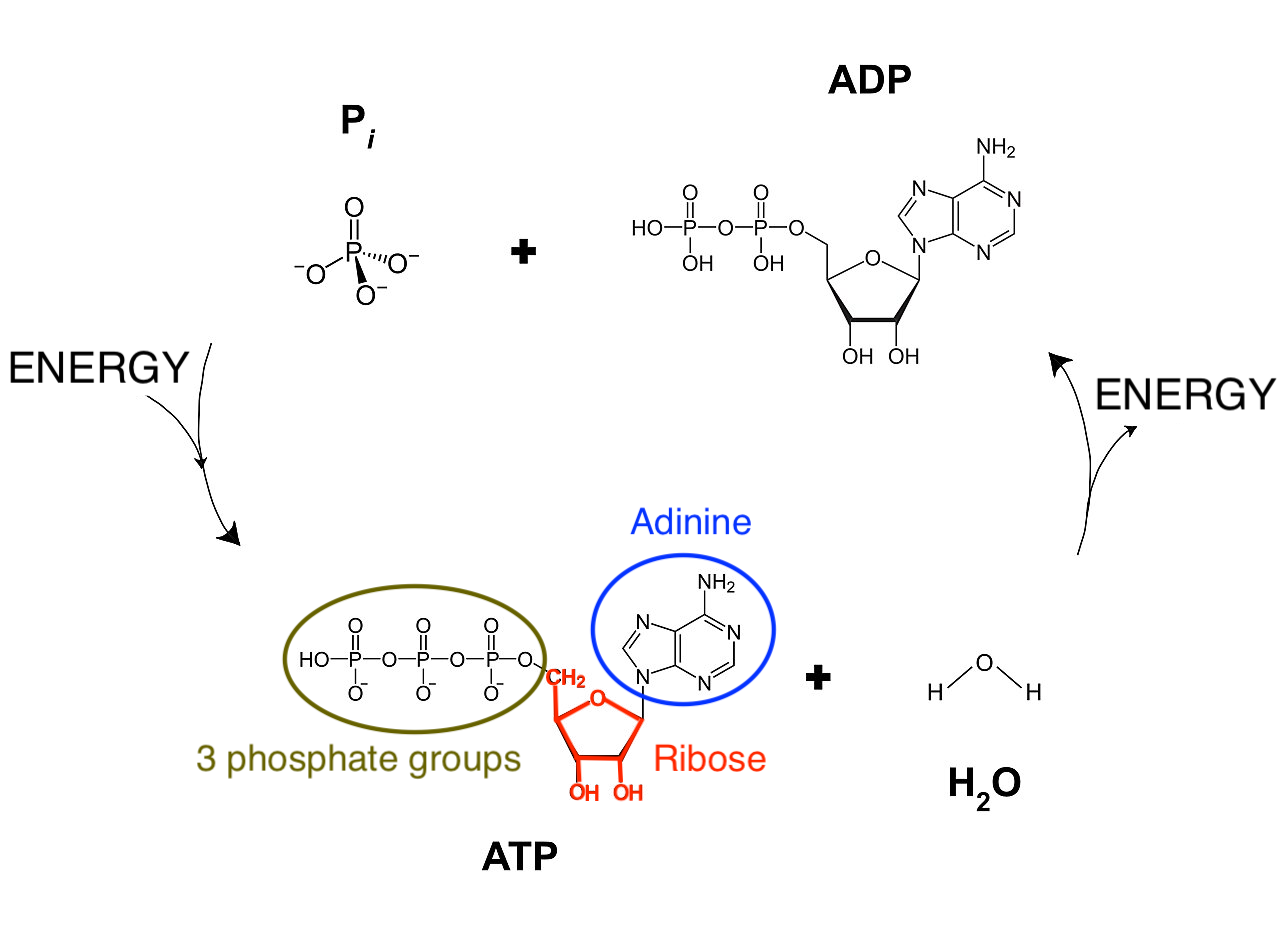
\includegraphics[width=0.7\linewidth]{./figs/ATP-ADP} 

}

\caption{Onze energiemunt ATP-ADP. Adinosine-trifosfaat (ATP) bestaat uit een basis adinine, een ribosesuiker en 3 fosfaatgroepen. Het splitsen van een fosfaatgroep van adinosine-trifosfaat (ATP) door een reactie met water (H\(_2\)O) resulteert in adinosine-difosfaat (ADP), een vrije fosfaatgroep, waarbij energie vrijkomt. Omgekeerd kan energie worden opgeslagen als chemische energie door een fosfaatgroep aan ADP te binden (bron: Aangepast van Wikipedia)}\label{fig:atp-adp}
\end{figure}

\pagebreak

\hypertarget{bouwstenen-van-het-leven}{%
\subsubsection{Bouwstenen van het Leven}\label{bouwstenen-van-het-leven}}

``Het leven is één'' omdat alle levende organismen zijn opgebouwd uit dezelfde fundamentele biomoleculen en we weten er allemaal meer over dan we denken, omdat we zijn wat we eten!

Bijna alle moleculen van levende organismen zijn samengesteld uit

\begin{itemize}
\tightlist
\item
  Lipiden, oliën en vetten, voor energieopslag en als bouwstenen voor membranen,
\item
  Koolhydraten, suikers, voor het opslaan van energie en als ruggengraat van grote biomoleculen,
\item
  Aminozuren, de bouwstenen van eiwitten die de werkpaarden van een cel zijn en het merendeel van de chemische reacties faciliteren, en
\item
  Nucleïnezuren, bouwstenen van RNA en DNA die worden gebruikt voor het opslaan, doorgeven en gebruiken van de genetische informatie die we van onze ouders erven.
\end{itemize}

Hieronder gaan we dieper in op elk van deze bouwstenen. Lezers die technische details willen overslaan, kunnen meteen gaan naar Sectie \ref{lifeChemistry} Leven is Chemie.

\hypertarget{lipiden}{%
\paragraph{Lipiden}\label{lipiden}}

\begin{figure}

{\centering 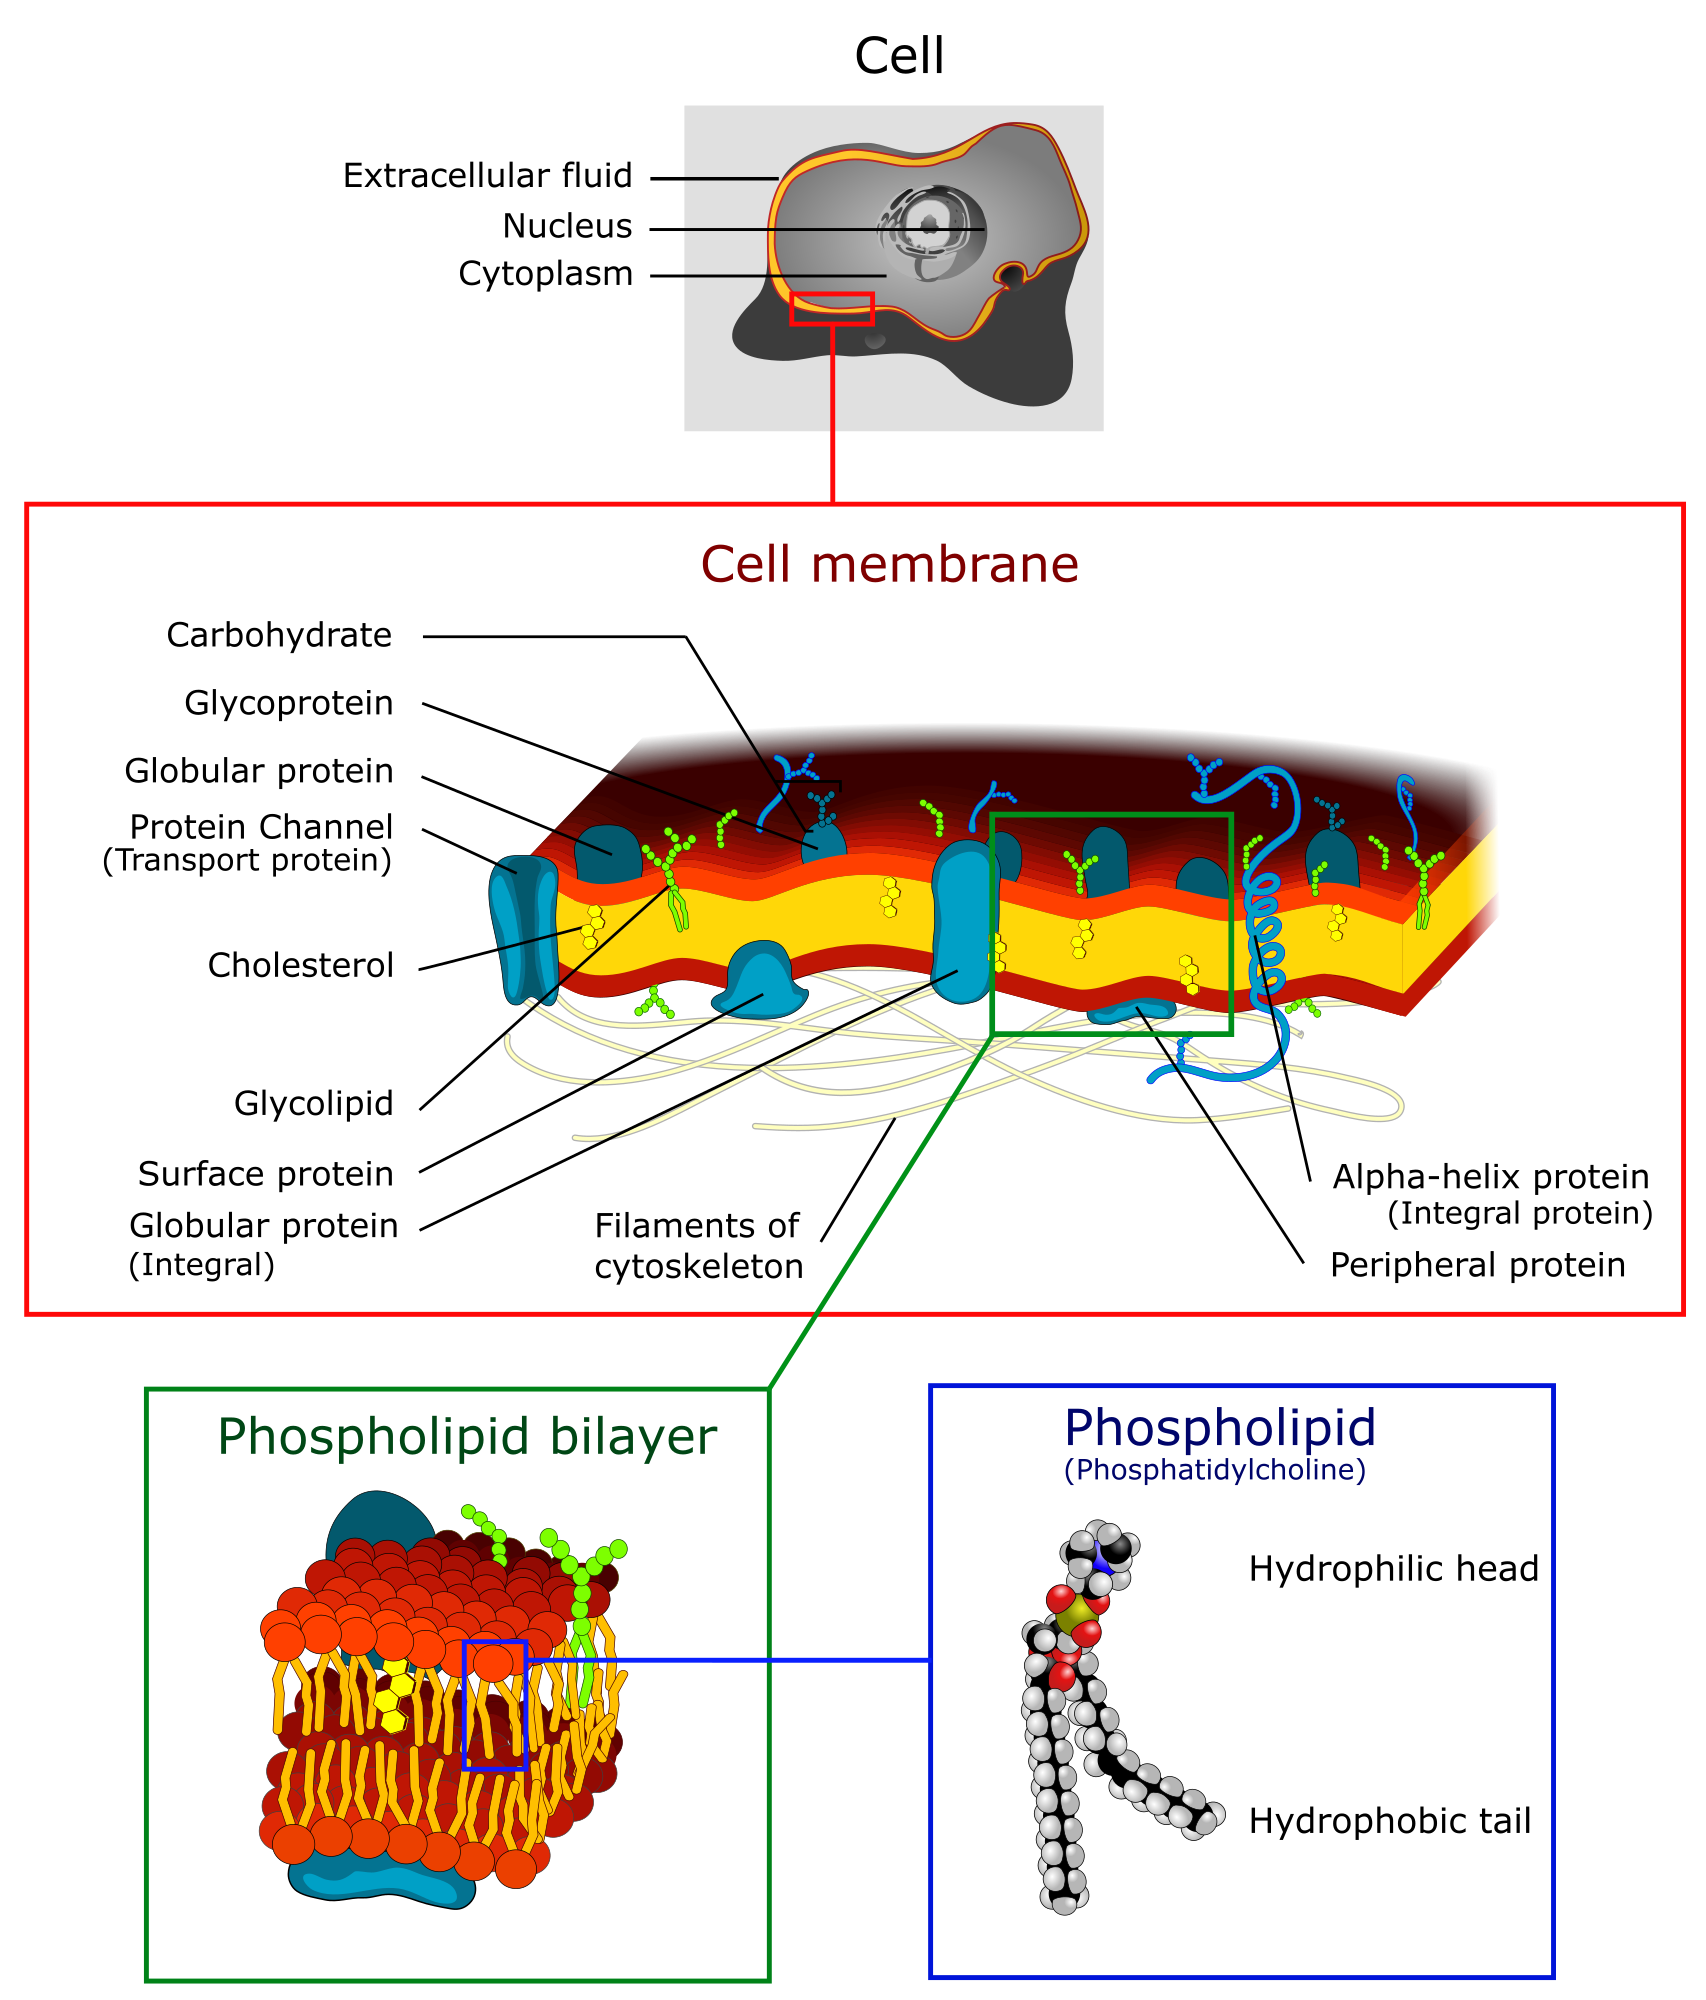
\includegraphics[width=0.8\linewidth]{./figs/Cell_membrane_detailed_diagram_4} 

}

\caption{Fosfolipiden spelen een zeer belangrijke rol in het leven omdat ze membranen vormen. Fosfolipiden hebben een hydrofiele kop die zich graag vermengt met water en lange hydrofobe staarten die zich niet vermengen met water. Ze geven spontaan aanleiding tot dubbellagen in waterige oplossingen, vergelijkbaar met de structuur die je in membranen ziet. Membranen zijn de grenzen van de cel en maken passieve diffusie van kleine moleculen door hun dubbellaag mogelijk. Grotere moleculen kunnen via membraaneiwitten actief worden uitgewisseld met de omgeving (Bron: Doug Hatfield, Wikipedia)}\label{fig:lipids}
\end{figure}

Lipiden, vetten en oliën worden gebruikt voor de opslag van energie, hormoonregulatie, doorgeven van zenuwimpulsen, bescherming van vitale organen en transport van vetoplosbare nutriënten. Bovendien zijn een belangrijke klasse van lipiden, de fosfolipiden, de bouwblokken voor de membranen van cellen en eencellige compartimenten die organellen worden genoemd, zie Figuur \ref{fig:lipids}. Fosfolipiden hebben inderdaad een polaire kop die zich graag in water bevindt en een lange apolaire staart die zich niet met water vermengt. Daarom worden in waterige oplossingen spontaan dubbellagen van fosfolipidemoleculen gevormd.

Membranen vormen de basis voor het concentreren van specifieke moleculen in (compartimenten van) levende cellen. Hierdoor kunnen cellen een onevenwicht van chemische moleculen opbouwen die werk kunnen verrichten terwijl een concentratiegradiënt spontaan dissipeert naar evenwicht. Fosfolipiden zijn dus van cruciaal belang voor het creëren van de randvoorwaarden die nodig zijn voor cellulaire organisatie.

\hypertarget{koolhydraten}{%
\paragraph{Koolhydraten}\label{koolhydraten}}

Koolhydraten zijn belangrijke biomoleculen die worden gebruikt voor opslag, energie en structuur (Figuur \ref{fig:carbohydrates}).

\begin{figure}

{\centering 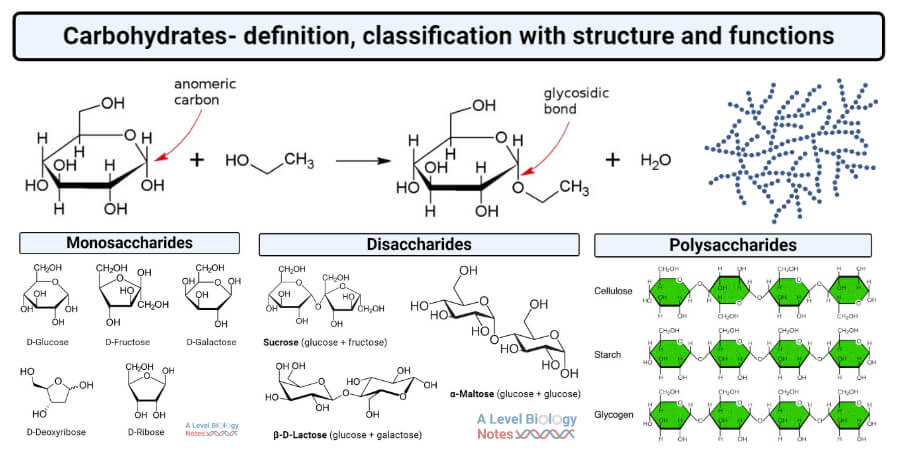
\includegraphics[width=1\linewidth]{./figs/Carbohydrates-definition-classification-with-structure-and-functions} 

}

\caption{Koolhydraten vervullen de belangrijke functies van opslag, energiebron en structuur. Ze kunnen worden georganiseerd in biopolymeren, lange ketens van koolhydraatmoleculen die aan elkaar zijn gebonden. De polysachariden zetmeel en glycogeen worden bijvoorbeeld gebruikt om energie op te slaan door respectievelijk plantaardige en dierlijke cellen. Cellulose daarentegen is een polysaccharide dat planten structuur geeft. Deoxyribose en ribose zijn belangrijke koolhydraten die respectievelijk de ruggengraat vormen van de biopolymeren DNA en RNA. (Bron: thebiologynotes.com)}\label{fig:carbohydrates}
\end{figure}

\begin{itemize}
\item
  Opslag: glucose wordt opgeslagen in dierlijke cellen met behulp van glycogeen, een polymeer van duizenden glucosemoleculen die aan elkaar gebonden zijn. Planten gebruiken een soortgelijk molecule: zetmeel.
\item
  Energiebron: specifieke eiwitten kunnen glycogeen en zetmeel splitsen in glucose, dat vervolgens wordt gemetaboliseerd voor energie.
\item
  Structuur: koolhydraten vormen de ruggengraat van veel biomoleculen; lange ketens van desoxyribose en ribose fungeren bijvoorbeeld als de ruggengraat van respectievelijk de biopolymeren DNA en RNA; en glucose is de ruggengraat van cellulose, die planten structuur geeft.
\end{itemize}

\hypertarget{sectionAminoAcids}{%
\paragraph{Aminozuren}\label{sectionAminoAcids}}

Aminozuren op zichzelf zijn eenvoudige moleculen (Figuur \ref{fig:aminoAcids}).
Hoewel er in het universum honderden aminozuren voorkomen, gebruikt het biologische leven er slechts twintig en combineert het ze in lange moleculen, polymeren, die eiwitten worden genoemd. Eiwitten zijn heteropolymeren, bestaande uit de 20 aminozuren die zijn gerangschikt in lange sequenties die van eiwit tot eiwit verschillen. In tegenstelling tot zetmeel, dat alleen uit glucosemoleculen bestaat die allemaal identiek zijn, zijn eiwitten dus ook dragers van informatie.



\begin{figure}

{\centering 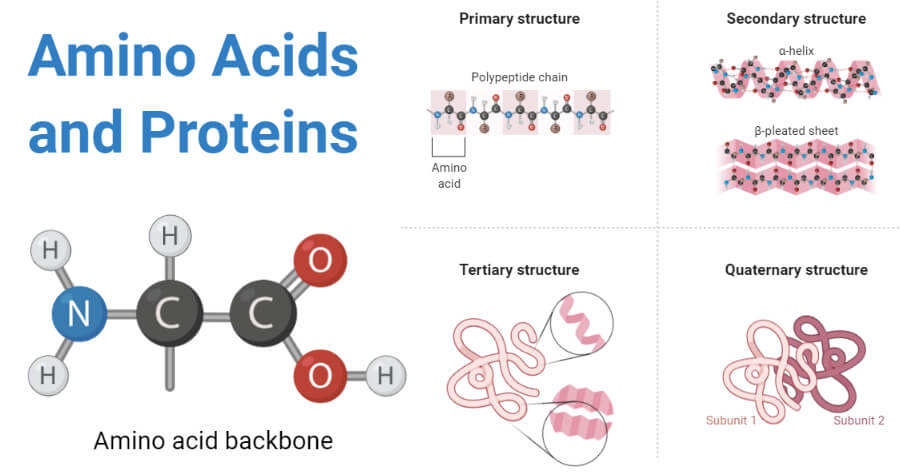
\includegraphics[width=1\linewidth]{./figs/Amino-acids-and-Proteins} 

}

\caption{Aminozuren zijn eenvoudige moleculen. Ze kunnen worden gecombineerd in lange moleculen, polymeren, ook wel eiwitten genoemd. Hun lange keten van aminozuren vouwt zich spontaan op in een complexe 3D-structuur die essentieel is voor hun biologische functie (Bron: thebiologynotes.com)}\label{fig:aminoAcids}
\end{figure}

Essentieel voor hun biologische functie van een eiwit is hoe zijn lange keten van aminozuren zich spontaan opvouwt tot een specifieke complexe 3D-structuur, die wordt bepaald door de eigenschappen en de specifieke volgorde van de aminozuren.

Veel eiwitten werken namelijk als een ``slot'' waarin specifieke (bio)moleculen als ``sleutel'' passen. Hierdoor kunnen eiwitten moleculen dicht bij elkaar brengen en chemische reacties bevorderen zonder te worden geconsumeerd. Dit proces wordt ook wel katalyse genoemd en eiwitten die katalyse uitvoeren worden enzymen genoemd, zie Figuur \ref{fig:enzyme}.

\begin{figure}

{\centering 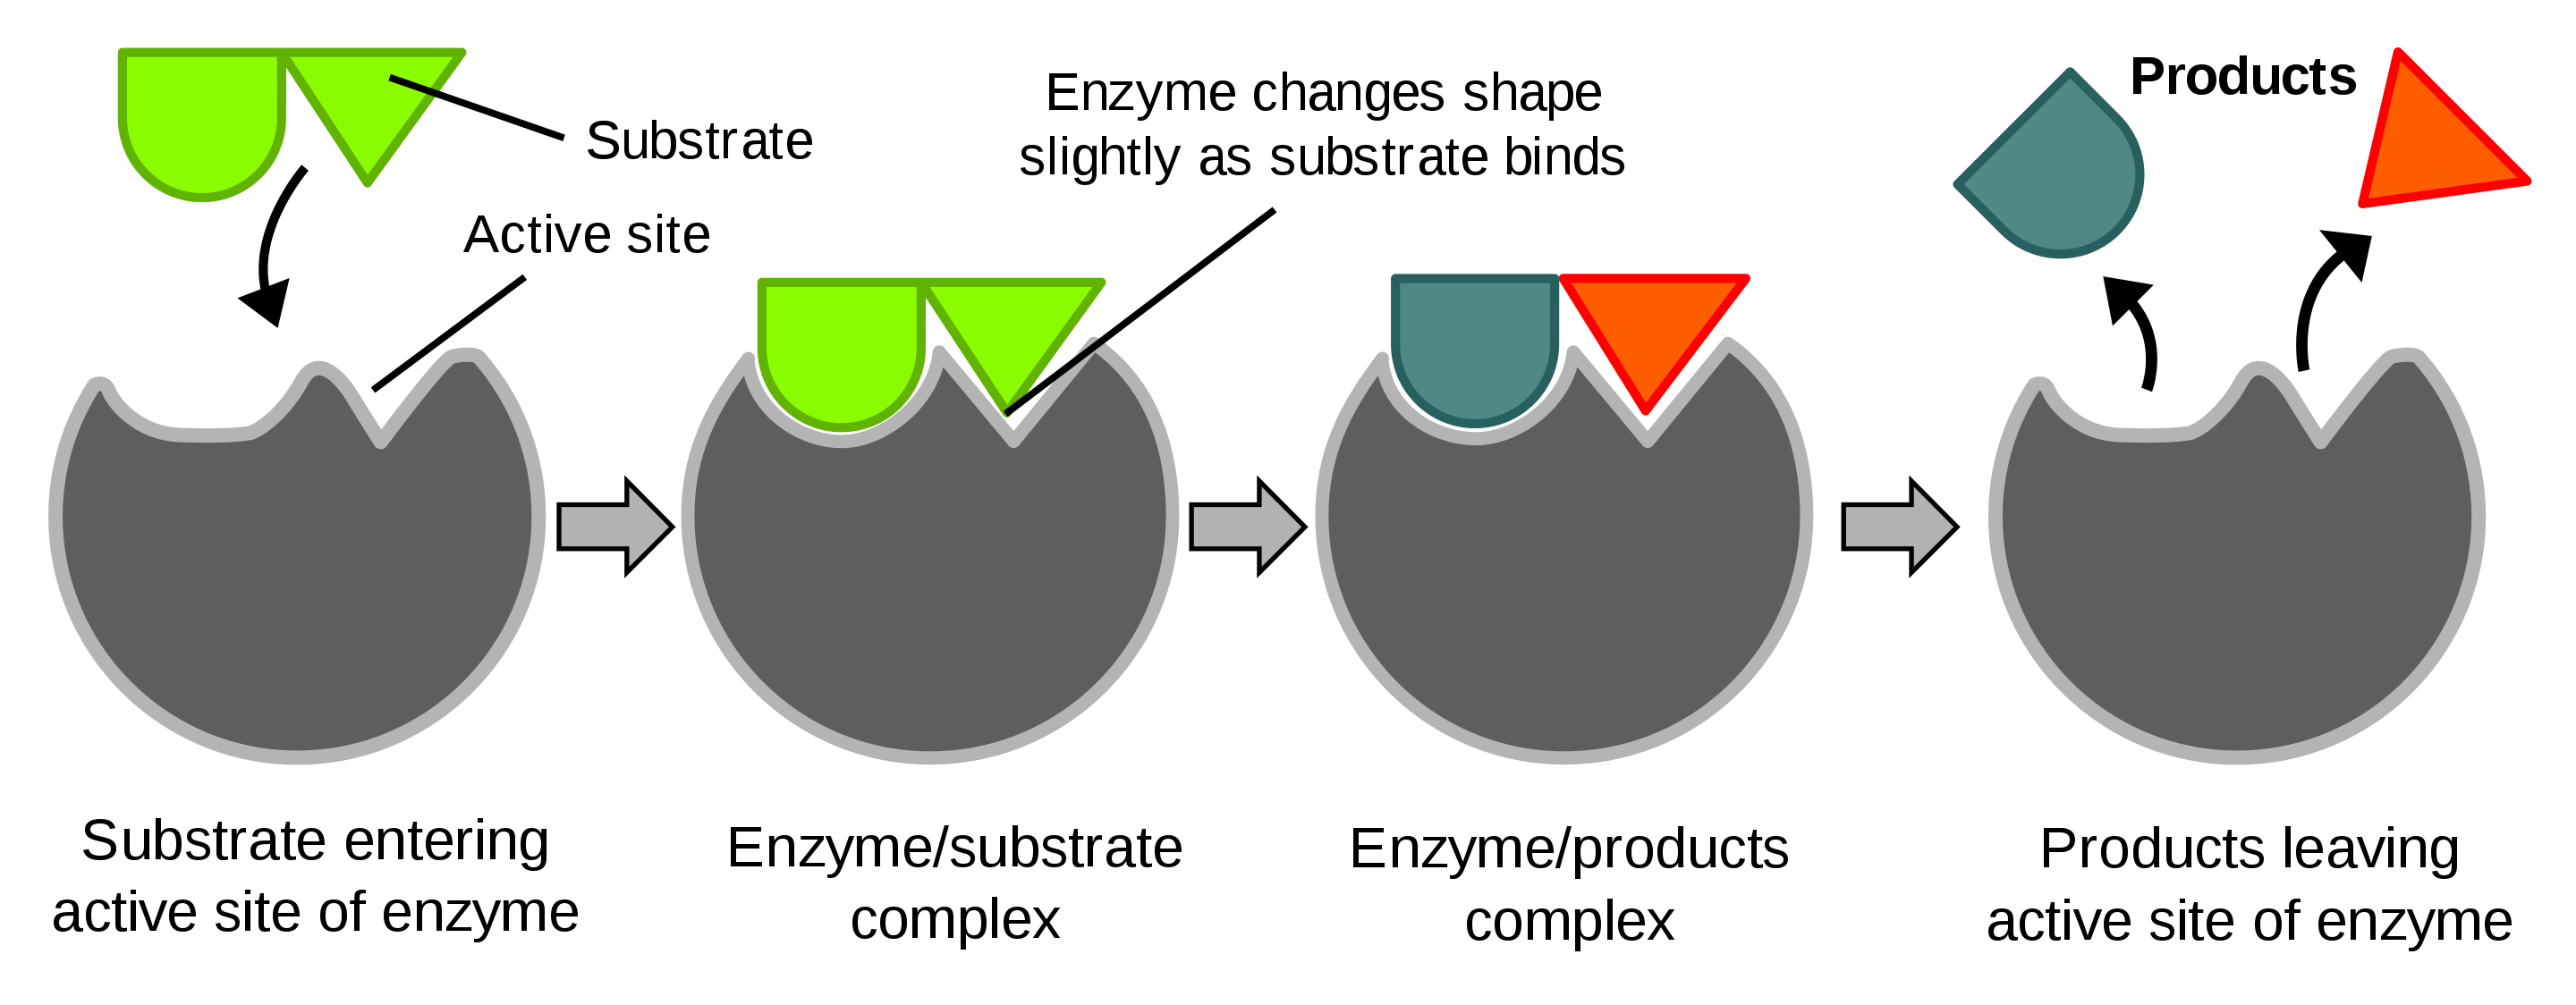
\includegraphics[width=0.5\linewidth]{./figs/EnzymePadlockKey} 

}

\caption{Diagram van een eiwit dat een enzymactie uitvoert (Bron: Wikipedia)}\label{fig:enzyme}
\end{figure}

Eiwitten zijn de belangrijkste werkpaarden van de cel en ze zijn belangrijk voor het verplaatsen van voedsel, het verteren van voedsel, het kopiëren van DNA, het geven van celstructuur, het beïnvloeden van de snelheid waarmee andere eiwitten werken, \ldots{}

\pagebreak

\hypertarget{sectionNucleicAcids}{%
\paragraph{Nucleïnezuren}\label{sectionNucleicAcids}}

Nucleïnezuren zijn opgebouwd uit nucleotiden. Elk nucleotide is samengesteld uit een van de vier stikstofhoudende nucleobasen, die de informatie dragen

\begin{enumerate}
\def\labelenumi{\arabic{enumi}.}
\tightlist
\item
  cytosine {[}C{]},
\item
  guanine {[}G{]},
\item
  adenine {[}A{]} of
\item
  thymine {[}T{]} (DNA) of uracil {[}U{]} (RNA) ,
\end{enumerate}

een fosfaatgroep en een suiker, met name ribose in ribonucleïnezuur (RNA, Figuur \ref{fig:RNA}) en deoxyribose in deoxyribonucleïnezuur (DNA, Figuur \ref{fig:DNA}).

Deze nucleotiden zijn de bouwstenen die worden gecombineerd in lange polymeren: RNA en DNA. DNA en RNA zijn heteropolymeren en de nucleotiden kunnen in elke volgorde worden gecombineerd. Ze kunnen dus informatie bevatten. Ze zijn inderdaad essentieel voor het opslaan, doorgeven en gebruiken van de genetische informatie die we van onze ouders erven.

DNA komt doorgaans voor als een dubbele streng, waarbij C en G, en A en T met elkaar hybridiseren met behulp van respectievelijk drie en twee waterstofbruggen om de iconische dubbelstrengige helixstructuur te vormen, zie Figuur \ref{fig:DNA}.

Er bestaat algemene consensus dat het leven waarschijnlijk begon met het gebruik van RNA als informatiedrager. DNA is echter veel stabieler en gaat langer mee in water dan RNA. Daarom is DNA waarschijnlijk later ontstaan en wordt het nu gebruikt om de genetische informatie in de meeste organismen op te slaan.

Het leven is ook één omdat we dezelfde genetische code delen, maar we verwijzen naar Sectie \ref{lifeInformation} ``Leven is Informatie'' voor meer details.

\begin{figure}

{\centering 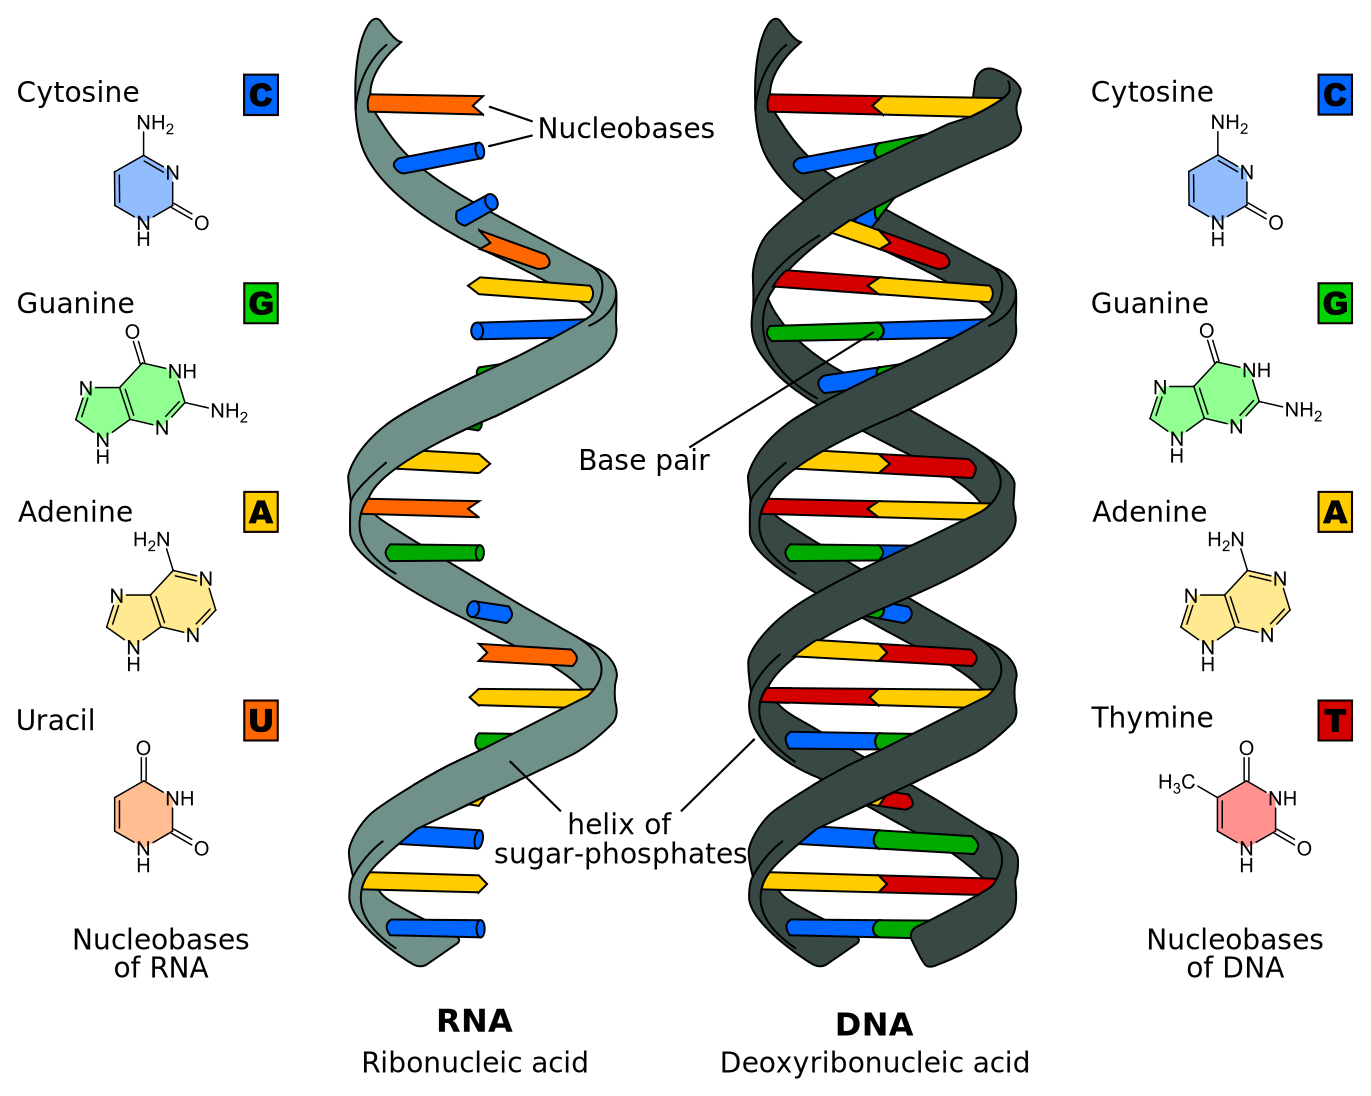
\includegraphics[width=0.5\linewidth]{./figs/Difference_DNA_RNA-EN} 

}

\caption{Nucleïnezuur: RNA (links) en DNA (rechts). RNA verschijnt doorgaans in een enkele streng en DNA als een dubbelstrengige molecule (Bron: Wikipedia)}\label{fig:RNAvsDNA}
\end{figure}

\begin{figure}

{\centering 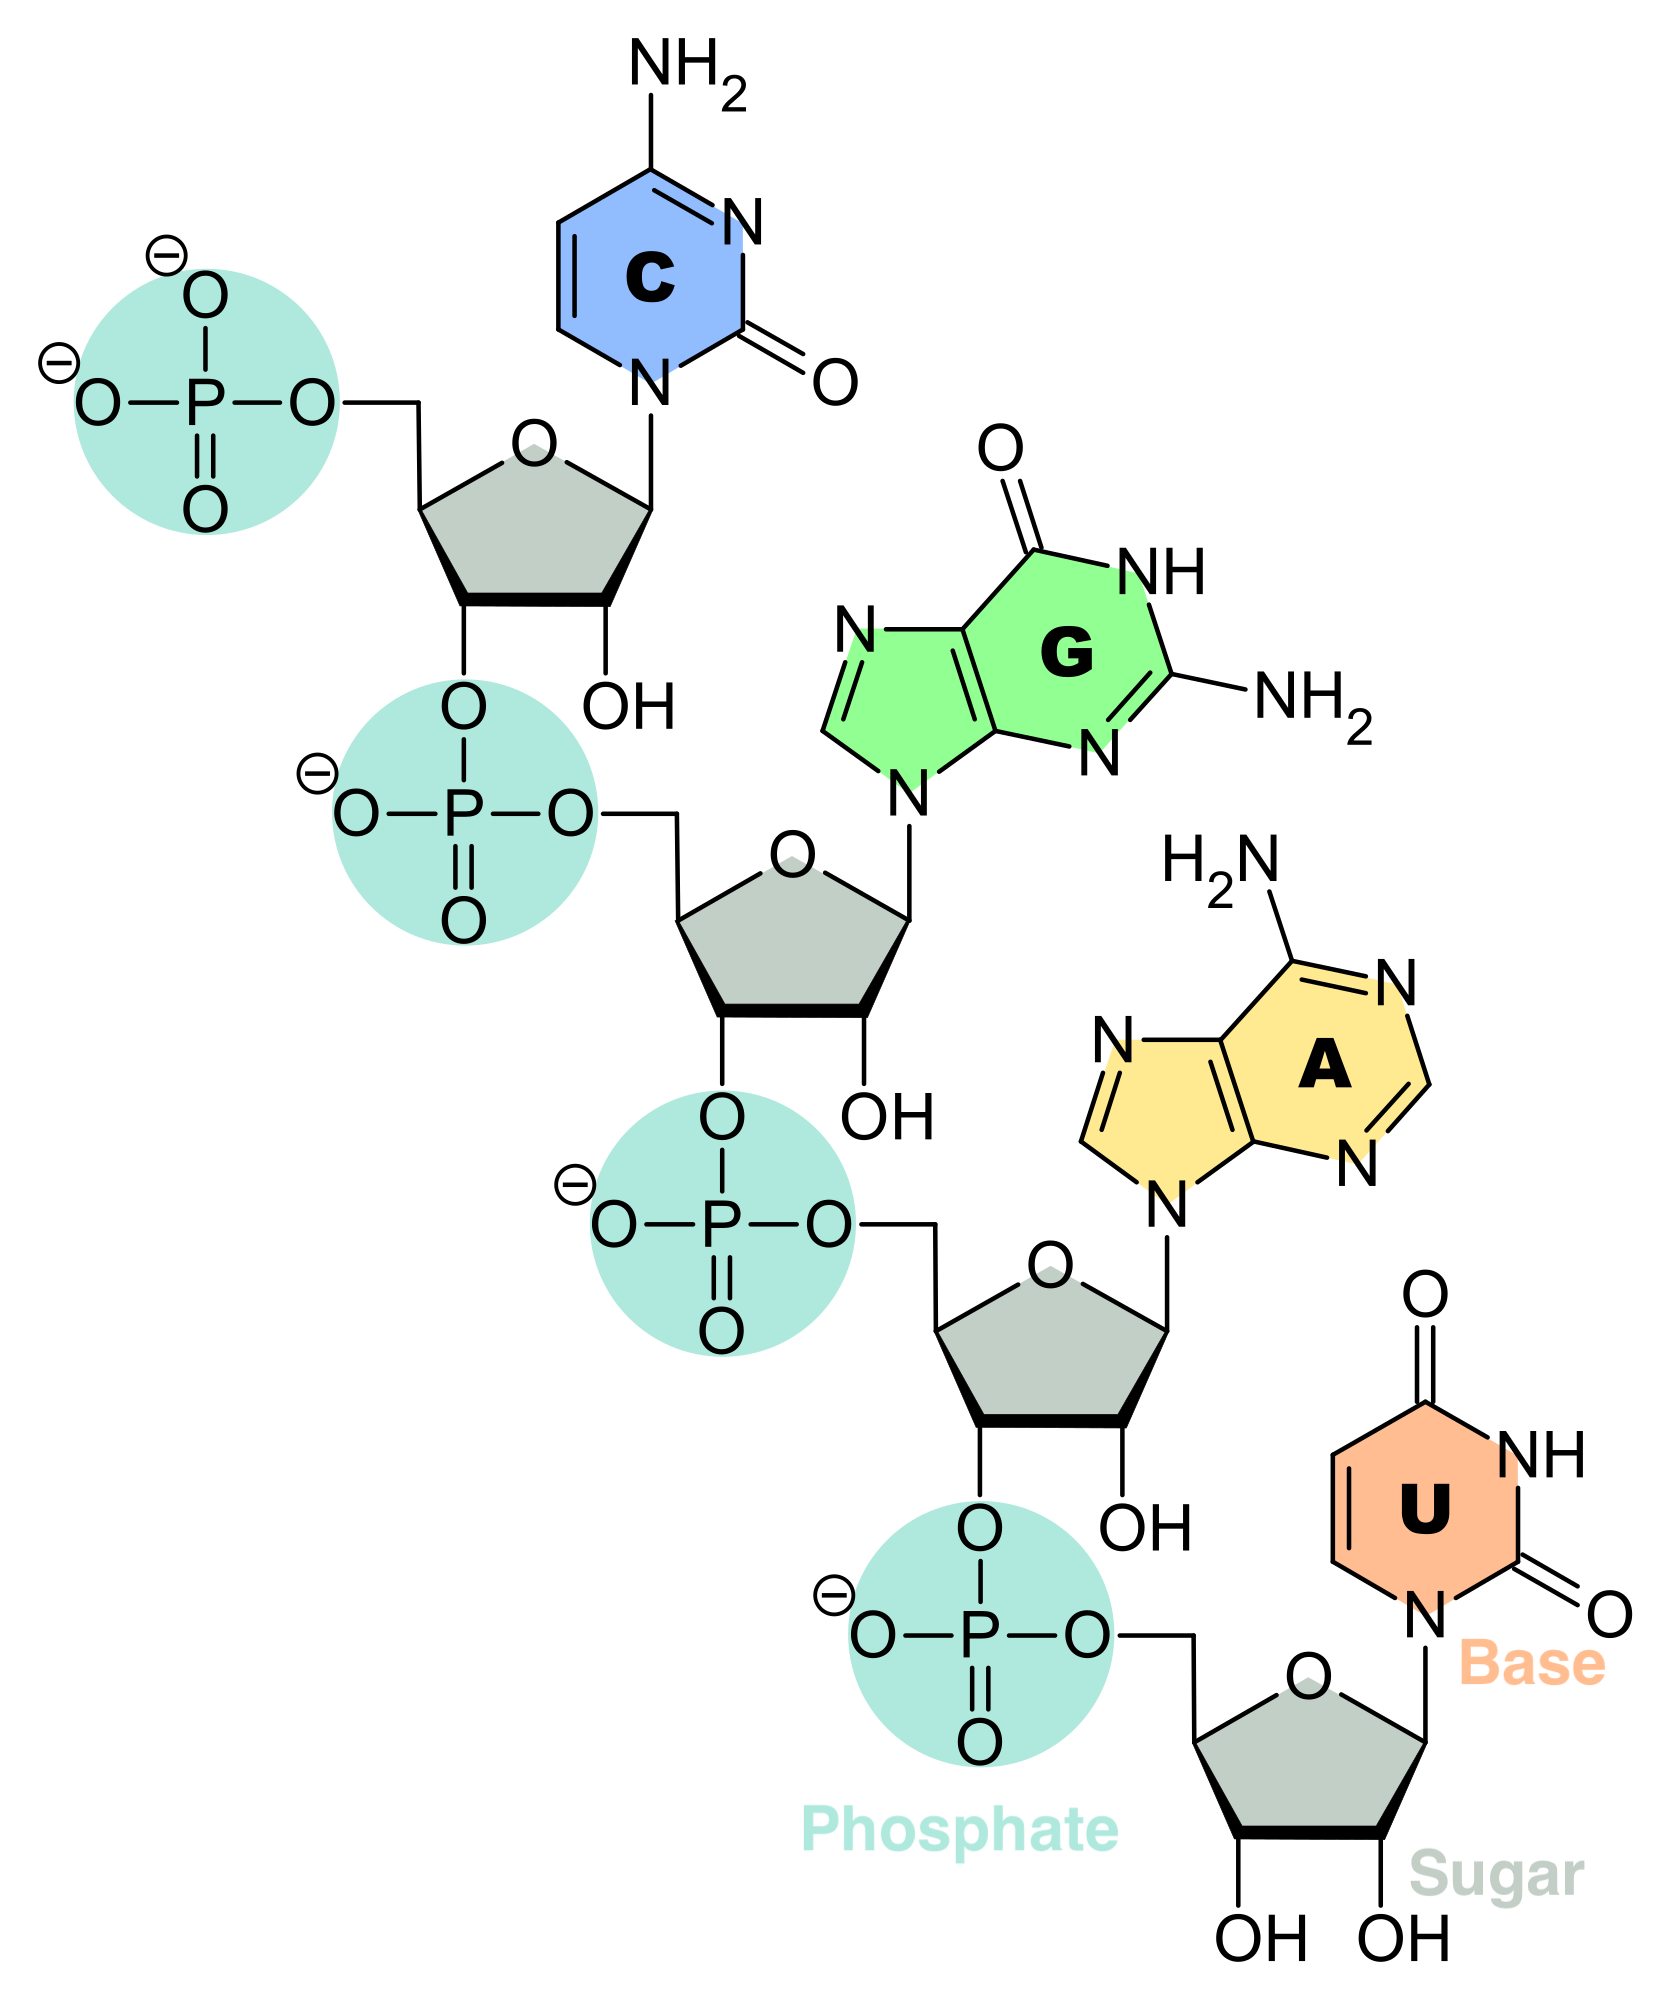
\includegraphics[width=0.5\linewidth]{./figs/RNA-Nucleobases} 

}

\caption{RNA is een biopolymeer met verschillende biologische rollen bij het coderen, decoderen, reguleren en expressie van genen. RNA bestaat uit een keten van nucleotiden. Elke nucleotide is opgebouwd uit een ribosesuiker die de ruggengraat vormt van het RNA-polymeer, een fosfaatgroep die wordt gebruikt om de ribosesuikermoleculen met elkaar te verbinden en een base adenine (A), cytosine (C), guanine (G) of uracil (U) die de dragers van informatie zijn. De basen kunnen waterstofbruggen vormen tussen cytosine en guanine, tussen adenine en uracil, en tussen adenine en thymine (een base uit DNA) (Bron: aangepast van Wikipedia)}\label{fig:RNA}
\end{figure}
\begin{figure}

{\centering 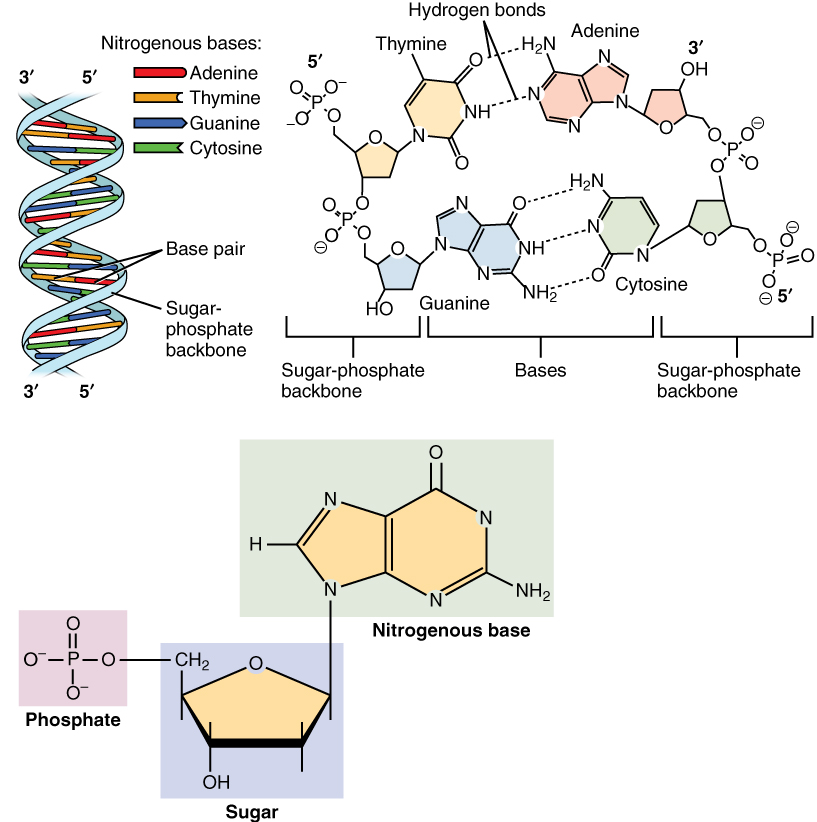
\includegraphics[width=0.5\linewidth]{./figs/DNA_Nucleotides} 

}

\caption{DNA is een polymeer dat bestaat uit twee polynucleotideketens die een dubbele helix vormen die genetische instructies bevat voor de ontwikkeling, het functioneren, de groei en de reproductie van alle organismen en veel virussen. Elke enkele DNA-streng bestaat uit een keten van nucleotiden. Elke nucleotide is opgebouwd uit een deoxyribosesuiker die de ruggengraat vormt van het DNA-polymeer, een fosfaatgroep die wordt gebruikt om de deoxyribosesuikermoleculen met elkaar te verbinden en een base adenine (A), cytosine (C), guanine (G) of thymine (T) die de dragers van informatie zijn. De basen vormen waterstofbruggen tussen cytosine en guanine, en adenine en thymine om vanuit enkelstrengig DNA een DNA dubbelstreng te vormen. (Bron: Wikipedia)}\label{fig:DNA}
\end{figure}

\newpage

\hypertarget{lifeChemistry}{%
\subsection{Leven is Chemie}\label{lifeChemistry}}

``Het leven is chemie'' omdat een cel bestaat uit een complex netwerk van chemische reacties die met elkaar verbonden zijn. Er bestaan veel feedbacklussen in de chemie van een cel, waardoor deze sterk niet-lineair is. De feedbacklussen zorgen ervoor dat een cel in zijn regime kan blijven (homeostase) of om kan schakelen van regime of attractor als reactie op externe en/of interne stimuli. Figuur \ref{fig:chemicalReactionsCell} geeft een overzicht van de meeste reacties in een levende cel. Ik heb dit overzicht alleen opgenomen om de lezer een idee te geven van de complexiteit en de rijkdom van de chemie in een individuele cel. U kunt inzoomen op deze kaart op \url{http://biochemical-pathways.com/\#/map/1}.

\begin{figure}

{\centering 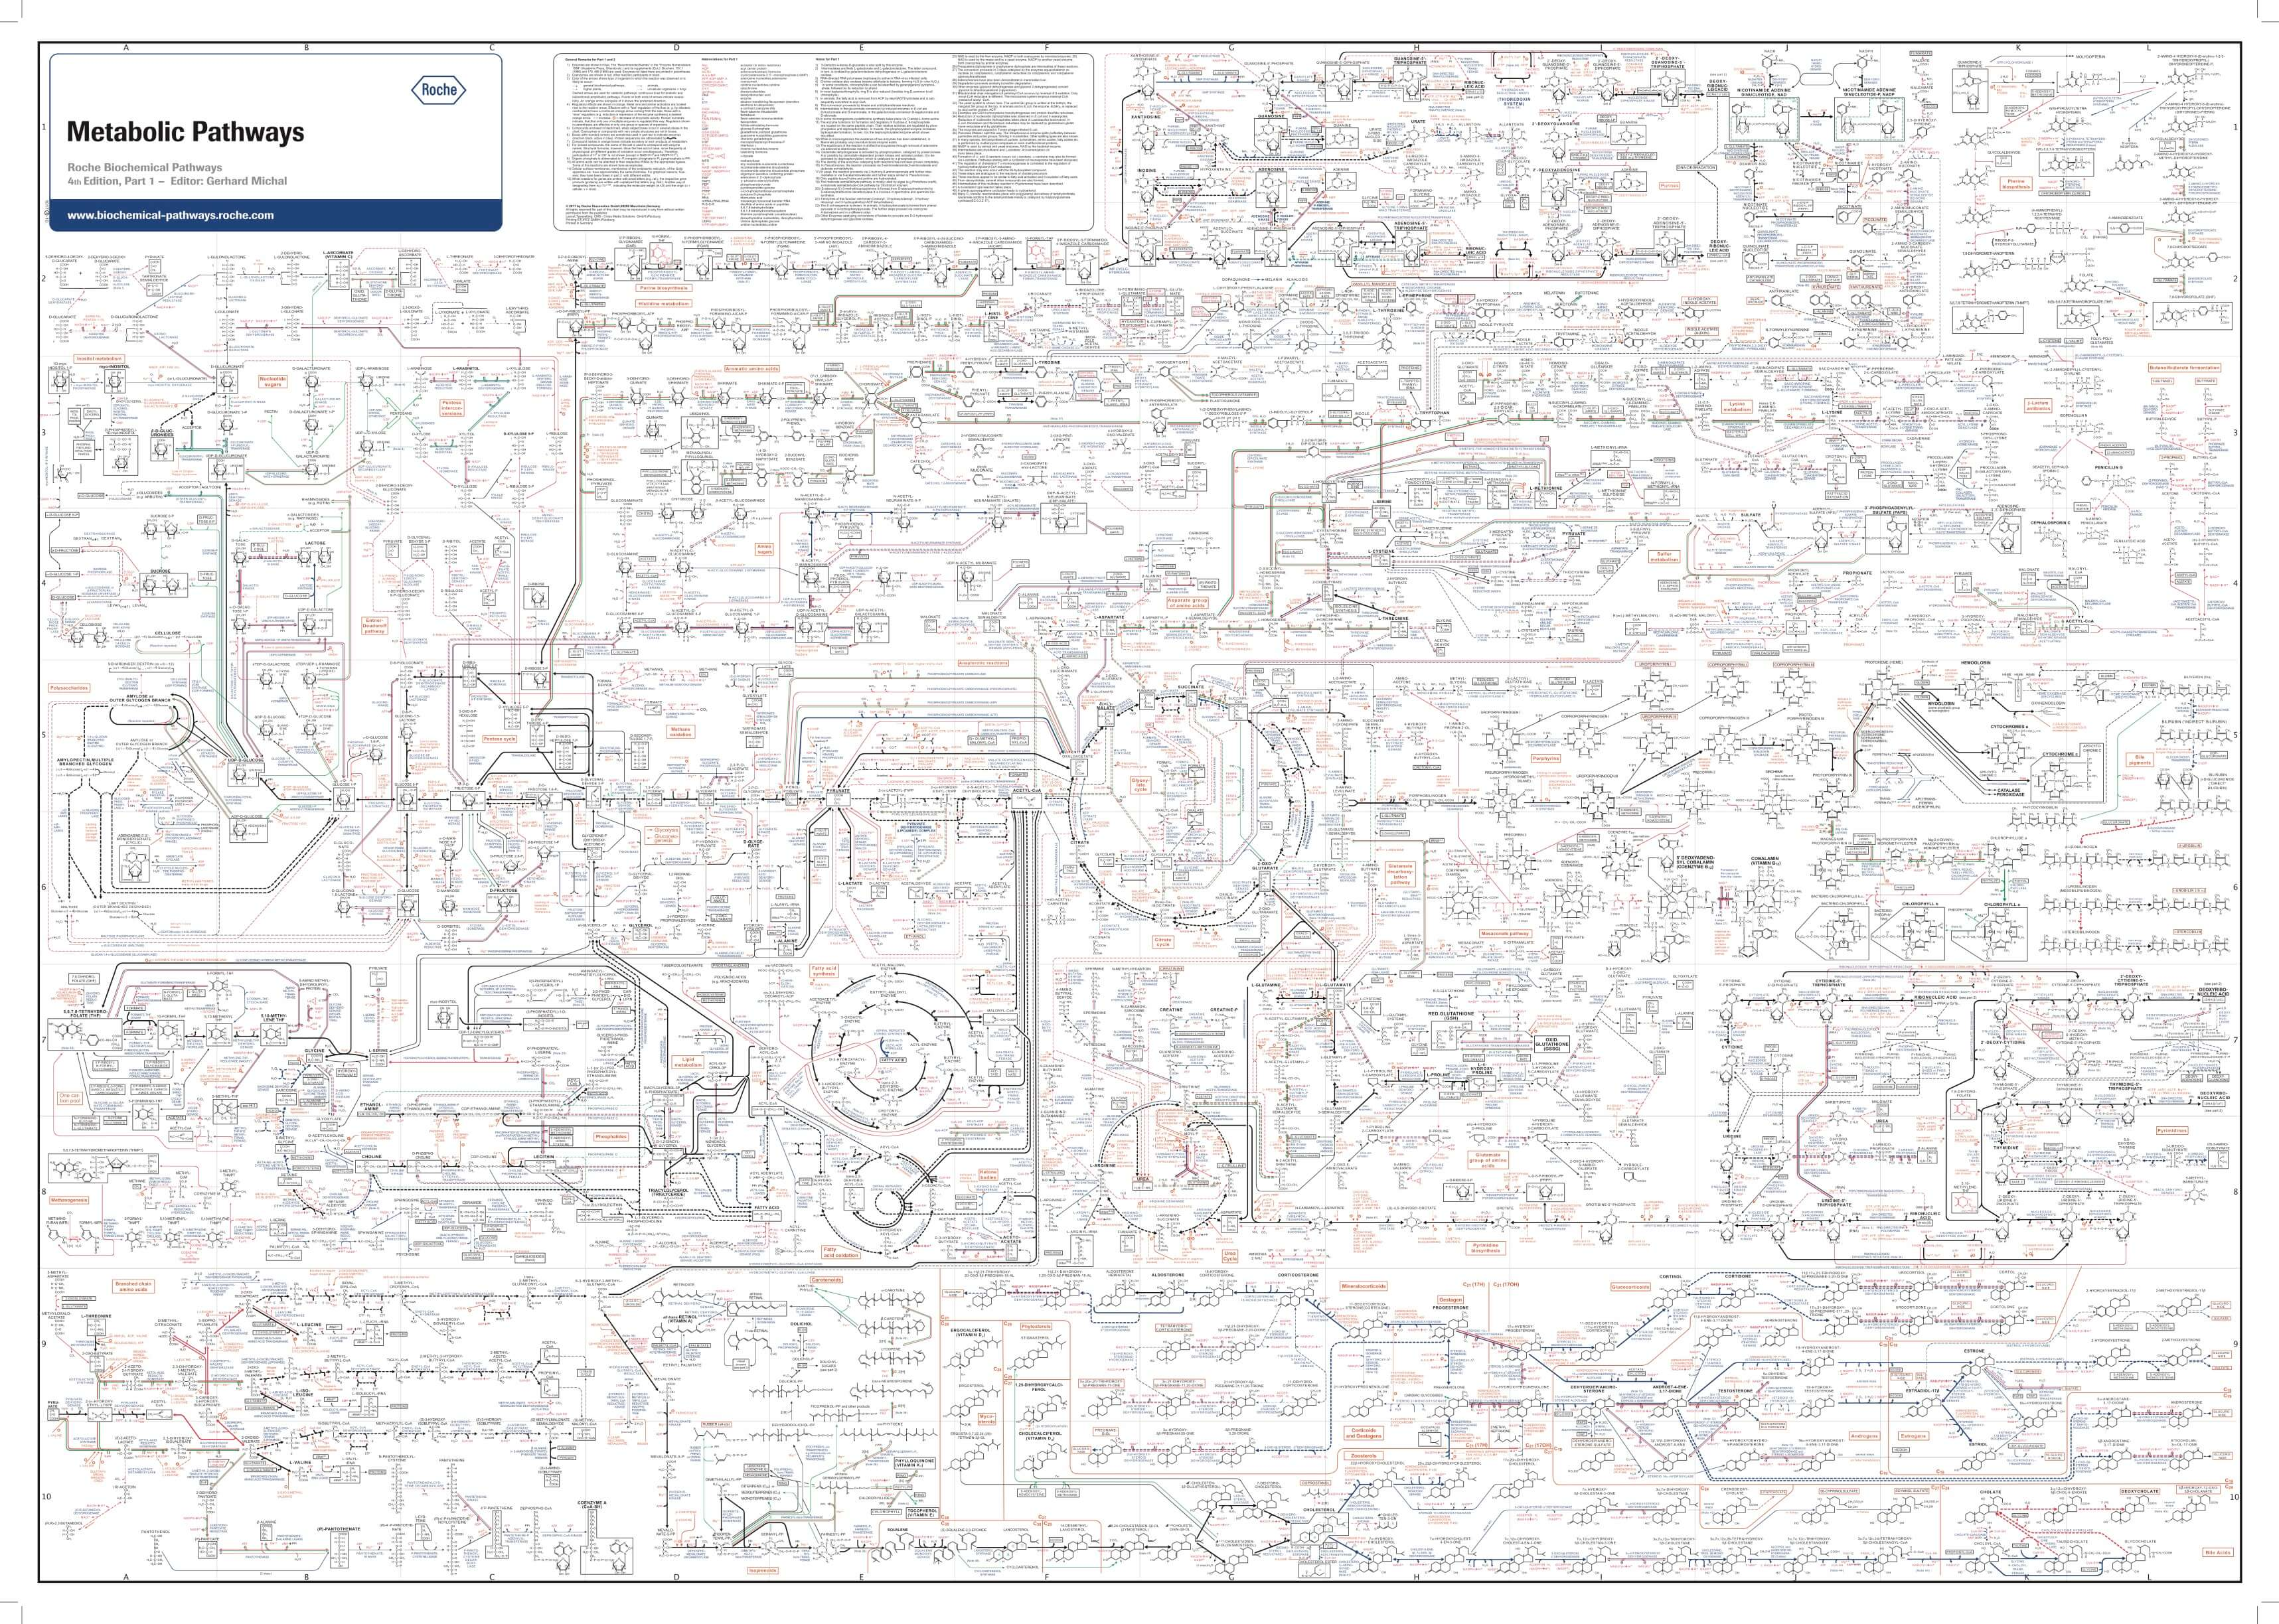
\includegraphics[width=1\linewidth]{./figs/roche_pathways} 

}

\caption{Netwerk van de belangrijkste reacties in een levende cel (Bron: Dr. Gerhard Michal, Roche)}\label{fig:chemicalReactionsCell}
\end{figure}

In het vervolg van deze sectie gaan we dieper in op energie en katalyse, en geven we ook een intrigerend voorbeeld van hoe eiwitten een rol spelen in de zelforganisatie van een cel. Lezers die technische details willen overslaan, kunnen direct gaan naar sectie \ref{lifeInformation} Leven is Informatie.

\hypertarget{energie}{%
\subsubsection{Energie}\label{energie}}

``Het leven is chemie'' omdat het chemische reacties gebruikt om energie op te slaan en te gebruiken, zie het ATP-ADP systeem in Sectie \ref{sectionEnergyCoin}.

\hypertarget{katalyse}{%
\subsubsection{Katalyse}\label{katalyse}}

Een katalysator is een chemische stof die ervoor zorgt dat een reactie plaatsvindt zonder dat deze wordt verbruikt. Eiwitten die katalysatoren zijn, worden ook wel enzymen genoemd.

Enzymen zijn eiwitten die

\begin{itemize}
\tightlist
\item
  de reactie initiëren
\item
  de reactie versnellen en
\item
  zorgen ervoor dat de uitkomst altijd hetzelfde is.
\end{itemize}

Losjes gezegd zullen ze

\begin{itemize}
\tightlist
\item
  bepaalde moleculen uit het complexe mengsel in een cel `vissen',
  dat bestaat uit duizenden chemische verbindingen, doorgaans in lage concentraties,
\item
  via bindingsplaatsen kunnen ze ervoor zorgen dat deze moleculen (substraten) dichtbij elkaar komen, zodat ze kunnen reageren en een nieuwe verbinding kunnen vormen.
\end{itemize}

Deze bindingsplaatsen kwamen voort uit de unieke 3D-structuur van het eiwit. In Figuur \ref{fig:enzyme} wordt een schematisch overzicht gegeven van de enzymwerking van een eiwit.

In de meeste gevallen werken enzymen samen in ``pathways'', die bestaan uit meerdere chemische reacties waarvoor (een deel van de) moleculen die in de vorige reactie zijn geproduceerd, door een ander enzym worden gebruikt om de volgende reactie te faciliteren.

De Krebs-cyclus is een bekend voorbeeld. Deze ``pathway'' is de belangrijke energiebron van een cel. Ze metaboliseert koolhydraten, lipiden en/of eiwitten (katabasis). De Krebs-cyclus is een cyclisch traject van meerdere chemische reacties, elk gekatalyseerd door een ander enzym (zie Figuur \ref{fig:krebsCycle} of de youtube clip \url{https://www.youtube.com/embed/yk14dOOvwMk}). De Krebs-cyclus genereert ook bouwstenen voor de opbouw van nucleotiden en aminozuren (anabasis). De Krebs-cyclus is dus opnieuw een voorbeeld van hoe anabasis en katabasis hand in hand gaan.

\begin{figure}

{\centering 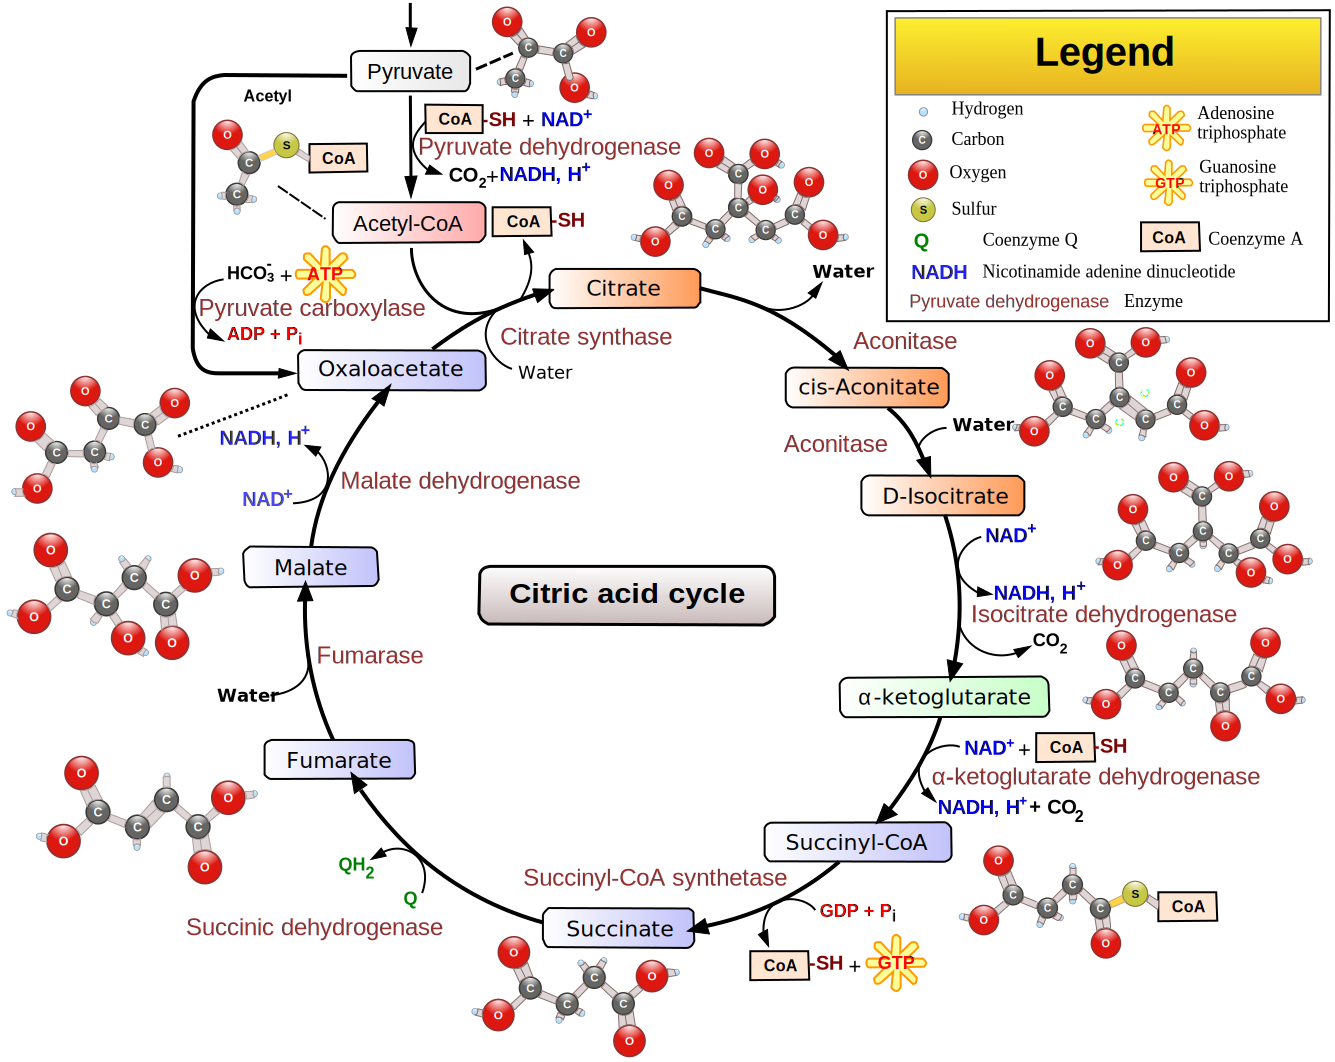
\includegraphics[width=0.7\linewidth]{./figs/Citric_acid_cycle_with_aconitate_2} 

}

\caption{ Krebs-cyclus, een cyclische pathway die energie produceert door koolhydraten, eiwitten en lipiden te metaboliseren en ter gelijkertijd nieuwe bouwblokken vormt voor nucleotiden en aminozuren. Elke reactie wordt gekatalyseerd door een enzym (Bron: Narayanese, Wikipedia)}\label{fig:krebsCycle}
\end{figure}

We kunnen dit gedeelte afsluiten met een citaat van \citet{deDuve2002}: ``Any living organism is a reflection of its enzyme arsenal''.

\hypertarget{zelf-organisatie}{%
\subsubsection{Zelf-Organisatie}\label{zelf-organisatie}}

Het leven wordt ook gekenmerkt door zijn vermogen tot zelforganisatie. Sommige eiwitten zijn ook belangrijk om structuur aan een cel te geven en kunnen spontaan structuur vormen. Een intrigerend voorbeeld van zelforganisatie wordt gegeven door \citet{Cheng2019} die Xenopus laevis eicel cytoplasma-extracten, de vloeistof met structuren uit de cel, eerst homogeniseerden. Het homogene extract reorganiseerde zichzelf spontaan in celachtige structuren binnen enkele minuten (zie Figuur \ref{fig:selforganisation} and you tube clip \url{https://www.youtube.com/embed/prq1Occu22s}).



\begin{figure}

{\centering 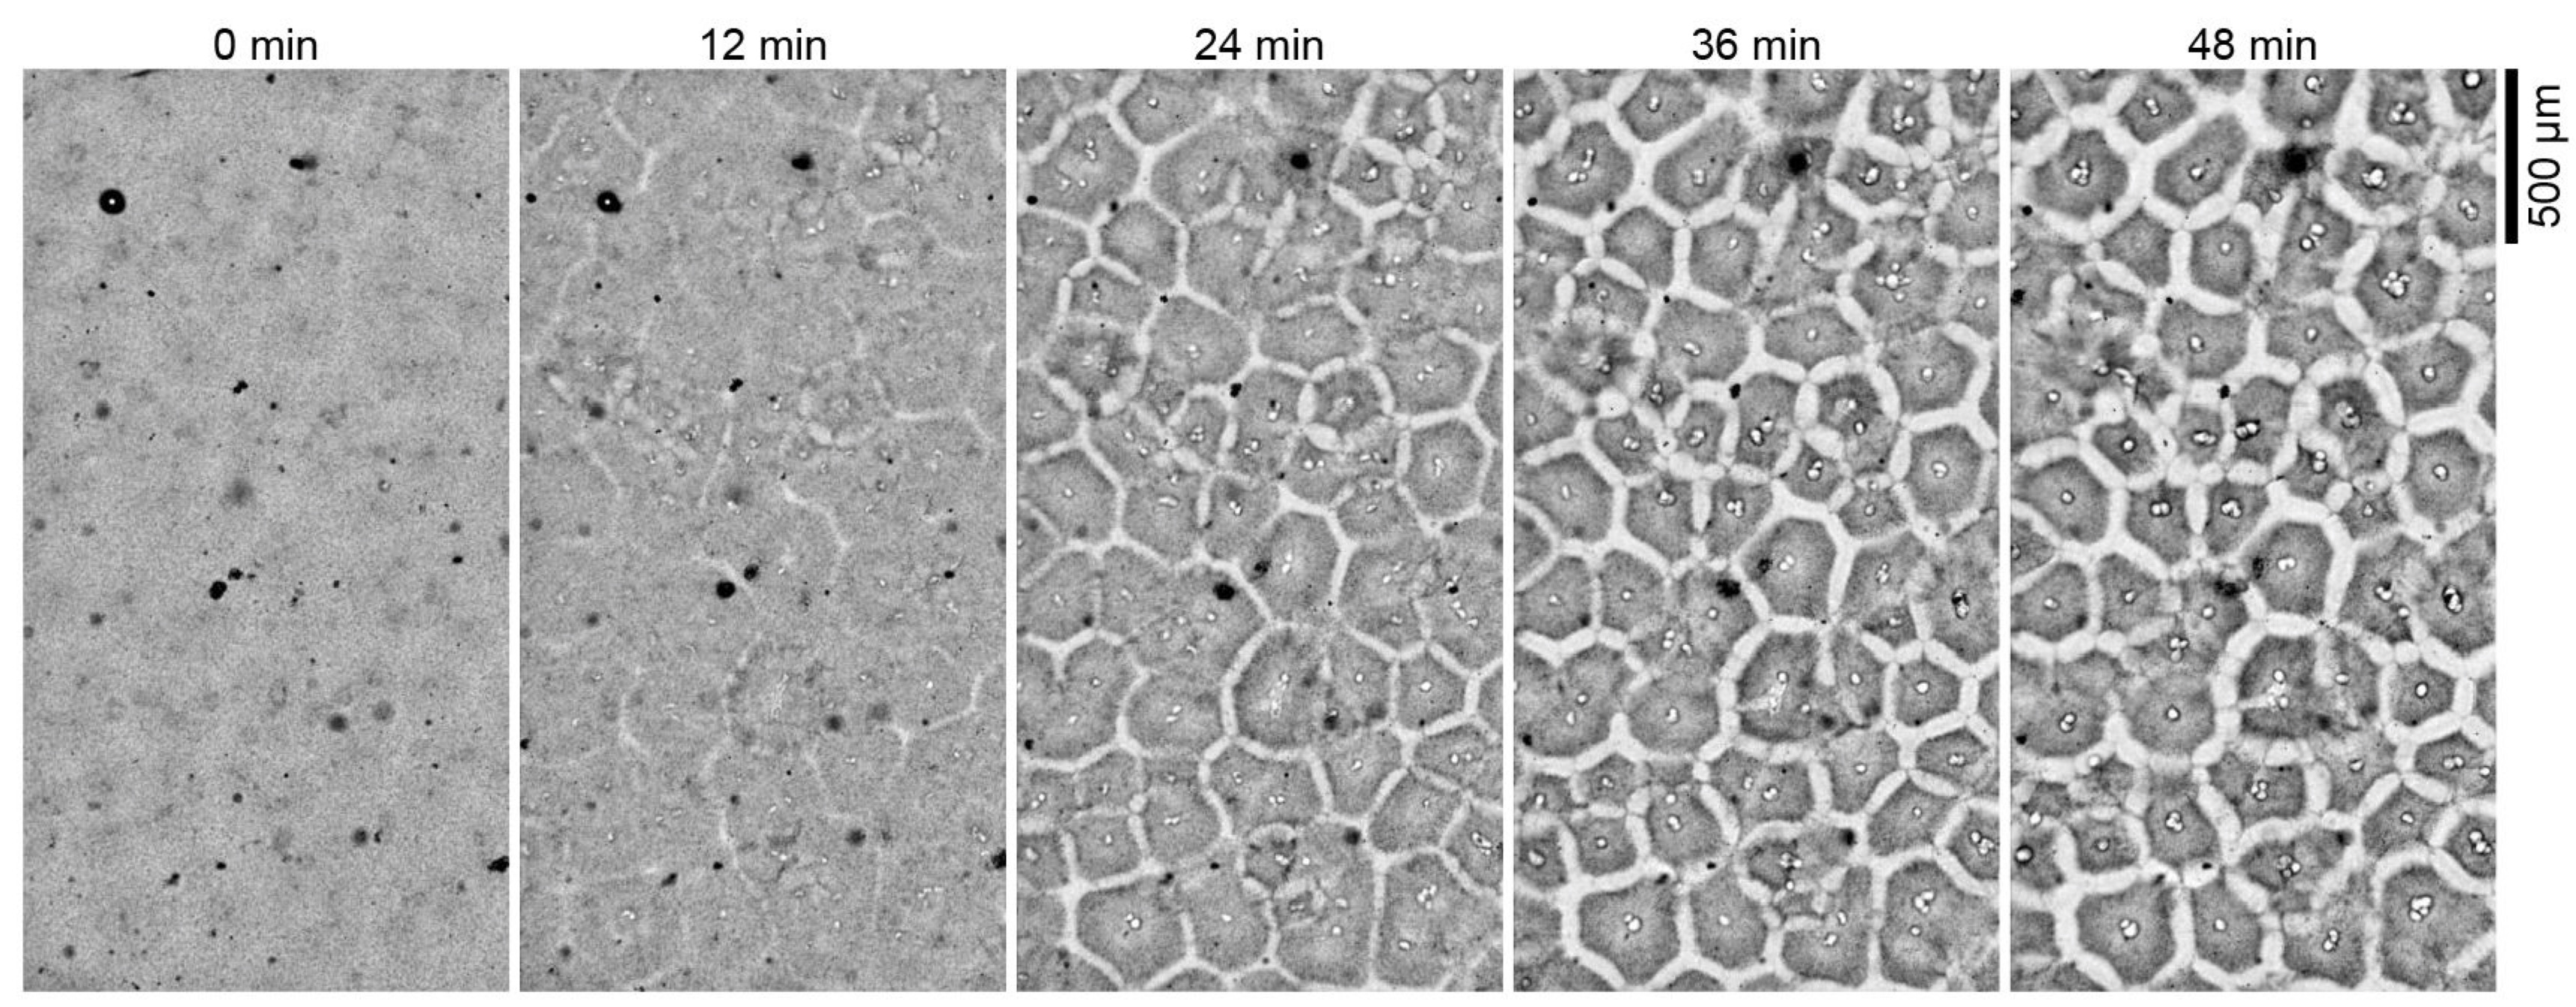
\includegraphics[width=1\linewidth]{./figs/selforganisation} 

}

\caption{Gehomogeniseerde eicytoplasmatische extracten van Xenopus laevis herorganiseren zich spontaan in celachtige compartimenten \citep{Cheng2019}}\label{fig:selforganisation}
\end{figure}

\citet{Cheng2019} ontdekten dat ATP, de energiedrager van een cel; microtubuli, een soort filamenteuze eiwitten; en dyneïne, een soort motoreiwit, nodig waren om dit proces van zelforganisatie aan te drijven.

\begin{figure}

{\centering 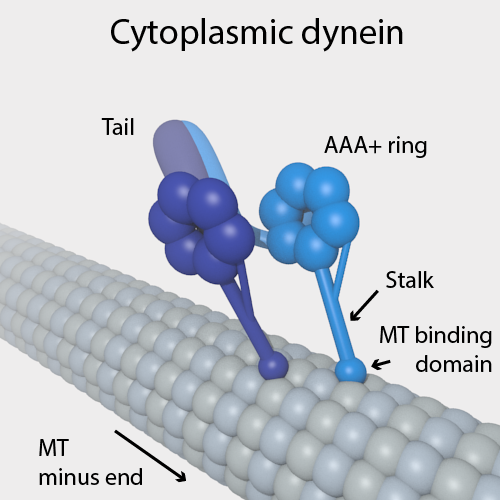
\includegraphics[width=0.3\linewidth]{./figs/DyneinHeavyChainOnMT} 

}

\caption{Microtubulus (long filamentous protein) with Dynein motor protein attached (Source:  Wikipedia)}\label{fig:dynein}
\end{figure}

Merk op dat eiwitten dus een centrale rol spelen in het leven. Ze zijn essentieel voor de katalyse en het geven van structuur. Een cel erft dus niet alleen genetische informatie, maar ook de ruimtelijke organisatie van een moedercel!

\hypertarget{lifeInformation}{%
\subsection{Leven is Informatie}\label{lifeInformation}}

Onze genetische informatie om al onze biomoleculen te bouwen, die we van onze ouders erven, is opgeslagen in ons DNA. DNA is een heteropolymeer of een lange keten van 4 verschillende bouwstenen, nucleotiden. De genetische informatie wordt dus opgeslagen in een alfabet van 4 letters. Dat zijn adenine (A), cytosine (C), guanine (G) en thymine (T) voor DNA.

Fysisch of chemisch gezien kunnen nucleotiden in om het even welke volgorde worden ingebouwd in DNA. Er is dus geen fysische of chemische basis voor de identiteit van het volgende nucleotide in de DNA-keten. Het is echter wel belangrijk voor onze biologie. Ons DNA kan daarom dus worden gezien als een coderingssysteem om genetische informatie op te slaan en door te geven van de ene generatie naar de volgende. Het leven is dus ook informatie en niet alleen maar chemie. Het is verbazingwekkend hoe variatie in de volgorde van deze ``vierlettercode'' kan leiden tot zo'n rijkdom aan verschillende kenmerken en functies die we waarnemen tussen verschillende individuen van dezelfde soort, alsook tussen individuen van verschillende soorten.

In rest van deze sectie geven we meer details over de informatiestroom in een cel. Lezers die technische details willen overslaan, kunnen onmiddellijk gaan naar Sectie \ref{maturanaVarela} Maturana en Varela: een Systeemvisie op het Leven.

\hypertarget{het-centrale-paradigma-van-de-moleculaire-biologie}{%
\subsubsection{Het Centrale Paradigma van de Moleculaire Biologie}\label{het-centrale-paradigma-van-de-moleculaire-biologie}}

Het `centrale paradigma' van de moleculaire biologie stelt dat de sequentie van nucleotiden in DNA eerst wordt afgelezen in RNA, ook transcriptie genoemd, en vervolgens wordt vertaald in eiwitten, ook wel translatie genoemd (Figuur \ref{fig:centralParadigm}).

Merk op dat sommige RNA-moleculen ook eindproducten zijn. RNA kan inderdaad ook een katalytische functie hebben, dat wil zeggen dat ze chemische reacties kunnen initiëren en bevorderen zonder te worden geconsumeerd.

Een \emph{gen} is de eenheid van genetisch materiaal, een DNA-sequentie die codeert voor de synthese van een genproduct, een eiwit of een functioneel RNA.

\begin{figure}

{\centering 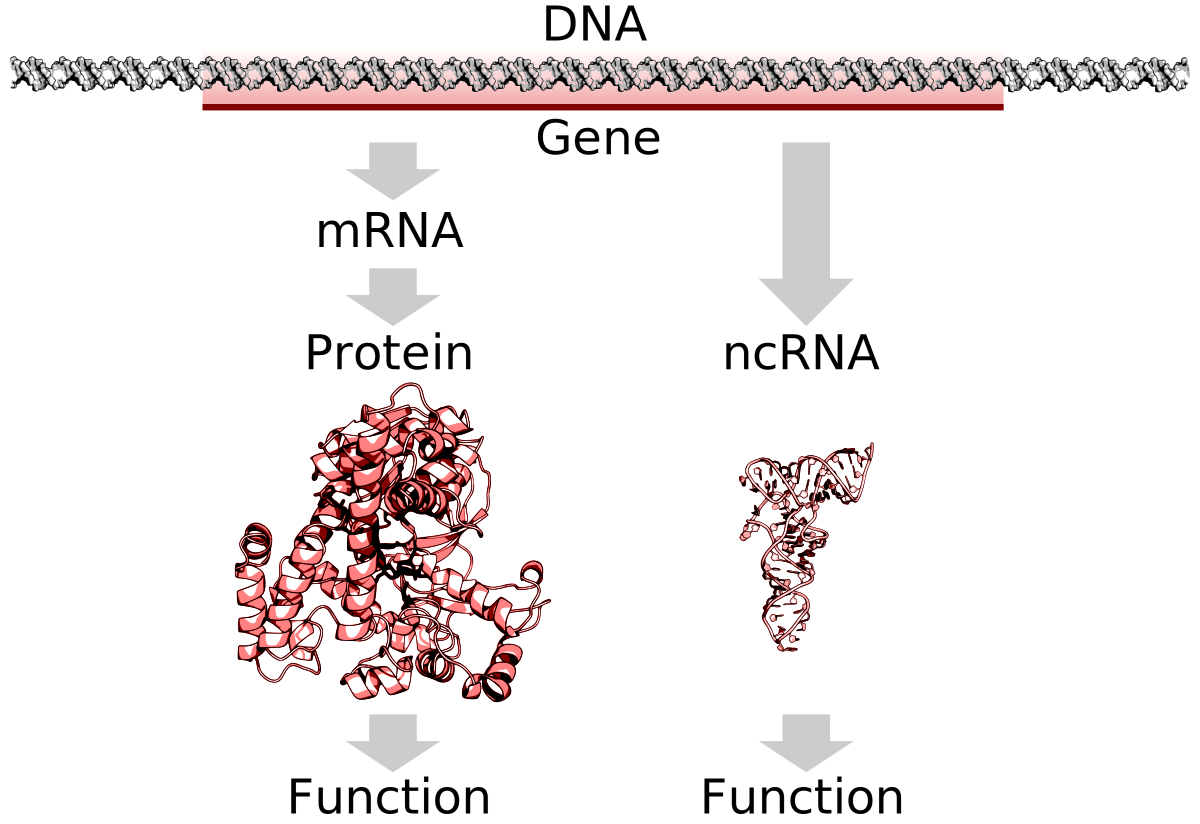
\includegraphics[width=0.5\linewidth]{./figs/gene} 

}

\caption{Centraal paradigma van de biologie: een gen, een specifiek gebied in het DNA, wordt eerst afgelezen in RNA en vervolgens vertaald in eiwitten. Merk op dat voor RNA-genen het RNA-molecule het eindproduct zelf is, ook wel niet-coderend RNA (ncRNA) genoemd (Bron:  Thomas Shafee, Wikipedia)}\label{fig:centralParadigm}
\end{figure}

Figuur \ref{fig:transcriptionTranslation} toont het proces van transcriptie van een gen van DNA naar RNA en de vertaling van RNA naar eiwitten.

\begin{enumerate}
\def\labelenumi{\arabic{enumi}.}
\item
  De transcriptie van DNA naar RNA wordt geïnitieerd door het openen van de dubbele DNA-streng. Vervolgens wordt een complementaire RNA-streng gesynthetiseerd door gebruik te maken van het feit dat A hybridiseert met U (of T) en G met C via waterstofbruggen.
\item
  Zodra de complementaire RNA-streng is gemaakt, wordt deze in de kern verder verwerkt tot messenger-RNA (mRNA). Het mRNA reist van de celkern naar het celcytosol (celvloeistof) waar het wordt vertaald in eiwitten en waar het merendeel van de reacties plaatsvindt.
\item
  Daar wordt mRNA door ribosomen vertaald in eiwitten. In de ribosomen wordt het mRNA gebonden aan tranfer RNA (tRNA). tRNA kan aan het mRNA-molecule binden als het 3 opeenvolgende nucleotiden heeft die complementair zijn aan het triplet van de 3 opeenvolgende nucleotiden op de mRNA-sjabloon die in het ribosoom ligt.
\item
  Het tRNA transporteert één specifiek aminozuur dat vervolgens wordt ingebouwd in het eiwit dat wordt gevormd: de groeiende aminozuurketen in Figuur \ref{fig:transcriptionTranslation}. De sequentie van drie opeenvolgende nucleotiden van het DNA van een gen wordt daarom ook wel een codon genoemd, omdat het codeert voor een specifiek aminozuur.
\item
  Na incorporatie van het aminozuur in de groeiende eiwitketen verschuift het ribosoom naar het volgende triplet van het mRNA en wordt het volgende tRNA eraan gebonden, enzovoort totdat een stopcodon wordt bereikt en het volledige eiwit is opgebouwd.
\end{enumerate}



\begin{figure}

{\centering 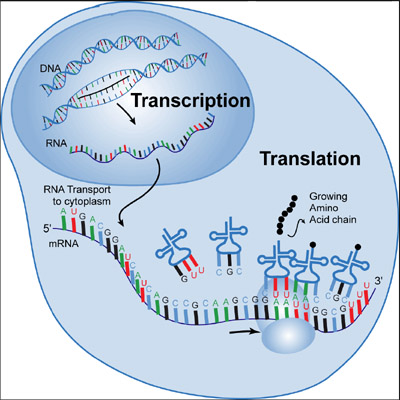
\includegraphics[width=0.5\linewidth]{./figs/transcription_2} 

}

\caption{In de celkern gaat de DNA-streng open en wordt afgelezen in een RNA-molecule. Na verwerking reist het boodschapper-RNA (mRNA) van de kern naar het cytosol, waar het wordt vertaald in eiwitten. Het mRNA is het sjabloon dat in een ribosoom past dat de functie heeft om transfer-RNA-moleculen aan het mRNA-sjabloon te binden. Het doet dat door te hybridiseren met een tRNA, dat een triplet van drie nucleotiden heeft die complementair zijn aan die van de mRNA-sjabloon. De tRNA's hebben een aminozuur aan hun staart, dat wordt ingebouwd in een lange keten van aminozuren, het eiwit dat wordt gevormd. Als het aminozuur is ingebouwd, gaat het ribosoom naar het volgende triplet en gebeurt het proces opnieuw met een nieuw tRNA (Bron: \href{http://www.tokresource.org/tok_classes/biobiobio/biomenu/transcription_translation/}{tokresources.org})}\label{fig:transcriptionTranslation}
\end{figure}

Er zijn in total 64=4\(^3\) codons die coderen voor elk van de 20 aminozuren, en voor een start- en een stopcodon om respectievelijk de eiwittranslatie te initiëren en te stoppen. Er is dus redundantie in de code, zie Figuur \ref{fig:codonTable}.

\begin{figure}

{\centering 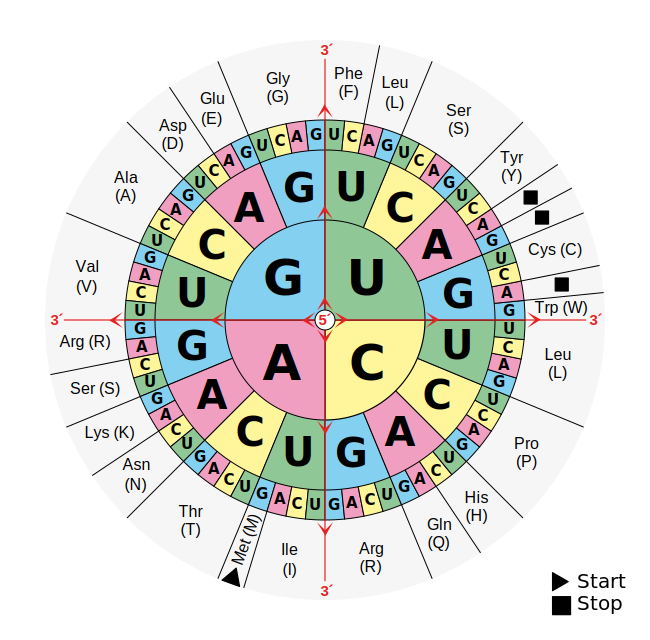
\includegraphics[width=0.5\linewidth]{./figs/Aminoacids_table} 

}

\caption{Codontabel die tripletten van nucleotiden verbindt met aminozuren (Bron: Wikipedia)}\label{fig:codonTable}
\end{figure}

Uit de codontabel leren we dat:

\begin{itemize}
\item
  Er is geen chemische noodzaak die de drie nucleotiden ``CGG'' expliciet verbindt met het aminozuur arginine in plaats van met glutamine. Hetzelfde geldt ook voor alle andere codons en hun respectievelijke aminozuren.
\item
  Nucleotiden zelf lijken dus geen chemische link te hebben met de aminozuren waarvoor ze coderen
\item
  Daarom noemen we het een code of informatie in plaats van alleen maar `genetische chemie'
\end{itemize}

De code is kennelijk zo geëvolueerd dat veel van de mutaties die ontstaan resulteren in

\begin{itemize}
\tightlist
\item
  synonieme codons die coderen voor hetzelfde aminozuur of
\item
  in codons voor aminozuren die vergelijkbaar zijn
\end{itemize}

zodat de eiwitfunctie behouden blijft.

In deze sectie leerden we dat DNA dus de drager is van genetische informatie. RNA speelt echter een meer centrale rol:

\begin{itemize}
\item
  Messenger RNA brengt de genetische informatie van de celkern naar het celcytosol, waar ze worden vertaald in eiwitten en waar de meeste chemische reacties plaatsvinden.
\item
  Ribozymen, katalytische RNA-moleculen, initiëren en versnellen bepaalde reacties
\item
  Transfer-RNA speelt een cruciale rol bij de vertaling van eiwitten
\item
  Een RNA-primer, een klein RNA-molecule, is essentieel om DNA te kopiëren
\item
  RNA fungeert ook als drager van genetische informatie, bijvoorbeeld bij het coronavirus.
\end{itemize}

\newpage

\hypertarget{maturanaVarela}{%
\section{Maturana en Varela: een Systeemvisie op het Leven}\label{maturanaVarela}}

In de reader van de Biodanza lerarenopleiding ``Module IV: Biologische Aspecten van Biodanza'' introduceerde Rolando Toro ook de term \emph{autopoiesis}.

\citet{capraLuisi2014} schrijven in hun boek ``The Systems View of Life'', dat de term werd geïntroduceerd door Varela and Maturana in the 1970s. ``Auto'', betekent ``zelf'' en refereert naar de autonomie van zelforganiserende systemen; en ``poiesis'' (die dezelfde Griekse oorsprong heeft als het woord poëzie) betekent ``makend''. Dus, ``autopoiesis'' betekent ``zelf-makend''.

Ze gaan daarna verder dat ``het belangrijkste kenmerk van het leven zelfbehoud is dankzij het interne netwerk van een chemisch systeem dat zichzelf voortdurend reproduceert binnen zijn eigen grenzen''.

Een levende cel is inderdaad de kleinste autopoëtische eenheid. De cel bestaat uit een complex intern netwerk van chemische reacties en dat binnen de grenzen van zijn buitenste membraan. Het kan zichzelf organiseren, in stand houden, kopieën van zichzelf maken en dit met de enzymatische arsenaal die in de cel zelf aanwezig is.

Netwerken van cellen worden vervolgens gecombineerd in grotere autopoëtische eenheden, b.v.

\begin{itemize}
\item
  ons darmmicrobioom dat bestaat uit een netwerk van miljarden eencellige bacteriën en gisten waaruit unieke metabolische functies voortkomen die essentieel zijn voor de vertering van ons voedsel, of,
\item
  onze weefsels, netwerken van onze eigen cellen waaruit nieuwe functies voortkomen, bijvoorbeeld ons denken dat voortkomt uit het complexe netwerk van neuronen in onze hersenen.
\end{itemize}

Een organisme of een biologisch systeem kan daarom niet worden gereduceerd tot zijn delen om er een volledig begrip van te krijgen. Een volledig begrip is alleen mogelijk als het als een geheel wordt beschouwd. Nieuwe functies op een hoger niveau komen voort uit het netwerk dat wordt gevormd tussen de delen van een lager niveau. Varela verwijst naar deze eigenschappen met de term \emph{emergente eigenschappen}.

\hypertarget{emergente-eigenschappen}{%
\subsection{Emergente Eigenschappen}\label{emergente-eigenschappen}}

Emergente eigenschappen worden op elk niveau teruggevonden. Op chemisch vlak, waar het eiwit hemoglobine bijvoorbeeld de unieke eigenschap heeft dat het zuurstof kan transporteren. Deze eigenschap komt voort uit zijn unieke 3D-structuur (zie Figuur \ref{fig:hemoglobin}). We hadden de biologische functie ervan op eiwitniveau nooit kunnen afleiden door het op te splitsen in de aminozuren waaruit het is opgebouwd en alleen de individuele eigenschappen van elk van deze aminozuren te bestuderen (zie Section \ref{sectionAminoAcids} voor meer details over aminozuren).

\begin{figure}

{\centering 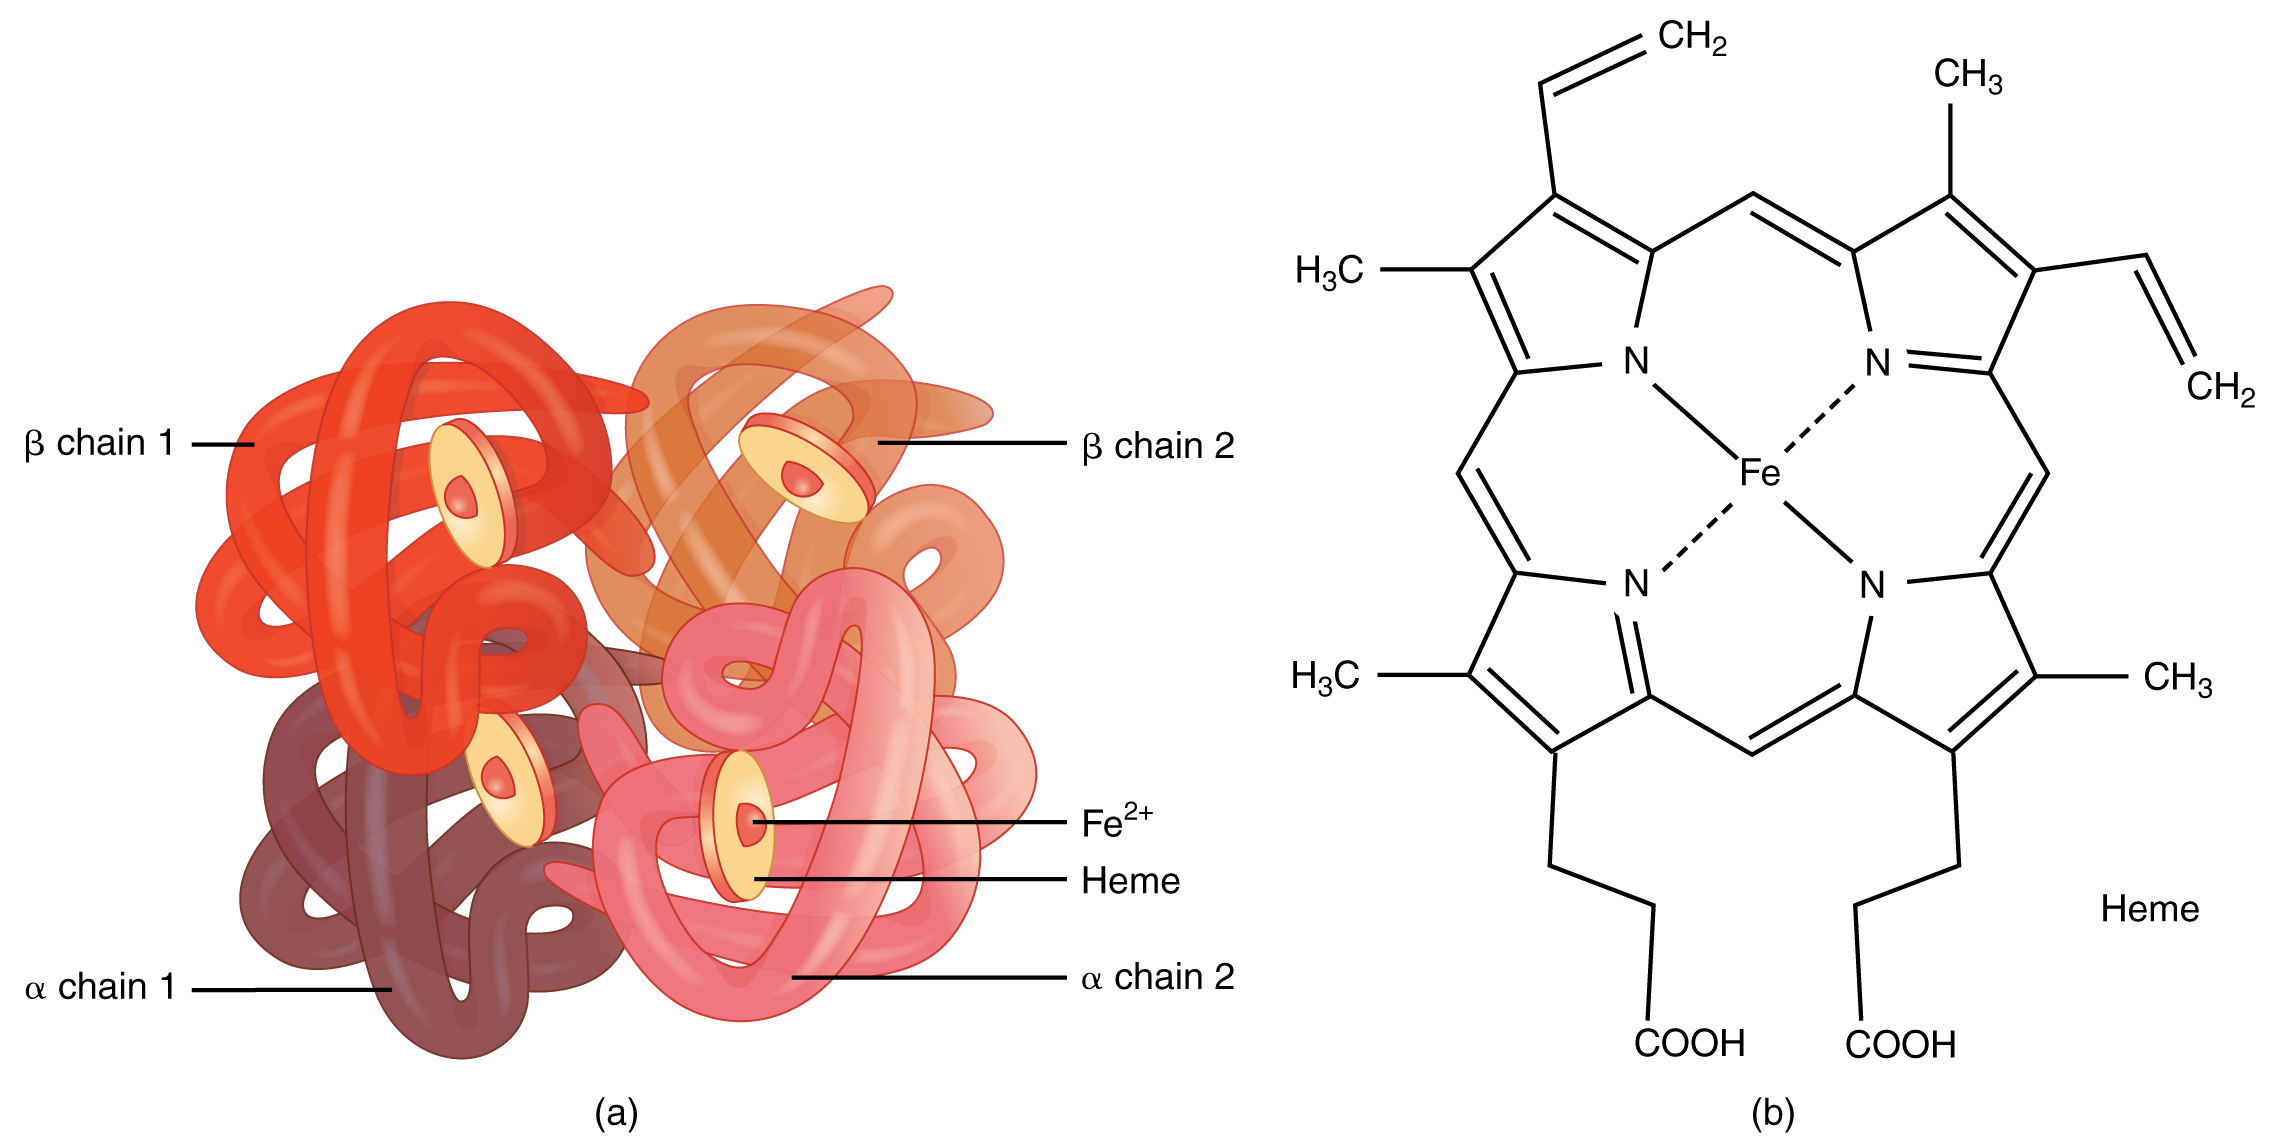
\includegraphics[width=1\linewidth]{./figs/hemoglobin} 

}

\caption{Structuur van hemoglobine dat bestaat uit 4 subeenheden, elk met een heemgroep met een ijzermolecule dat zuurstof kan binden. Deze functie komt voort uit zijn unieke 3D-structuur (Bron:  Wikipedia)}\label{fig:hemoglobin}
\end{figure}

De eigenschap van hemoglobine om zuurstof te transporteren komt dus spontaan voort door de specifieke volgorde van de eenvoudige aminozuurmoleculen waaruit het eiwit is opgebouwd: deze specifieke lange keten van aminozuren vouwt zich spontaan op tot een unieke 3D-structuur die het hemoglobine-eiwit zijn speficieke functie geeft.

\pagebreak

Korstmossen zijn een ander overtuigend voorbeeld van emergente eigenschappen (Figuur \ref{fig:lichen}). Korstmossen zijn echte kolonisten. Ze behoorden tot de eerste organismen die het aardoppervlak koloniseerden. Wanneer gletsjers zich terugtrekken, verschijnen er korstmossen op de kale rotsen en in de loop van duizenden jaren kunnen ze deze rotsen omzetten in aarde, een omgeving die vruchtbaar is voor andere soorten. Hun unieke en belangrijke eigenschappen voor het leven op aarde hadden we echter nooit kunnen verwachten als we alleen de componenten van een korstmos zouden bestuderen.

\begin{figure}

{\centering 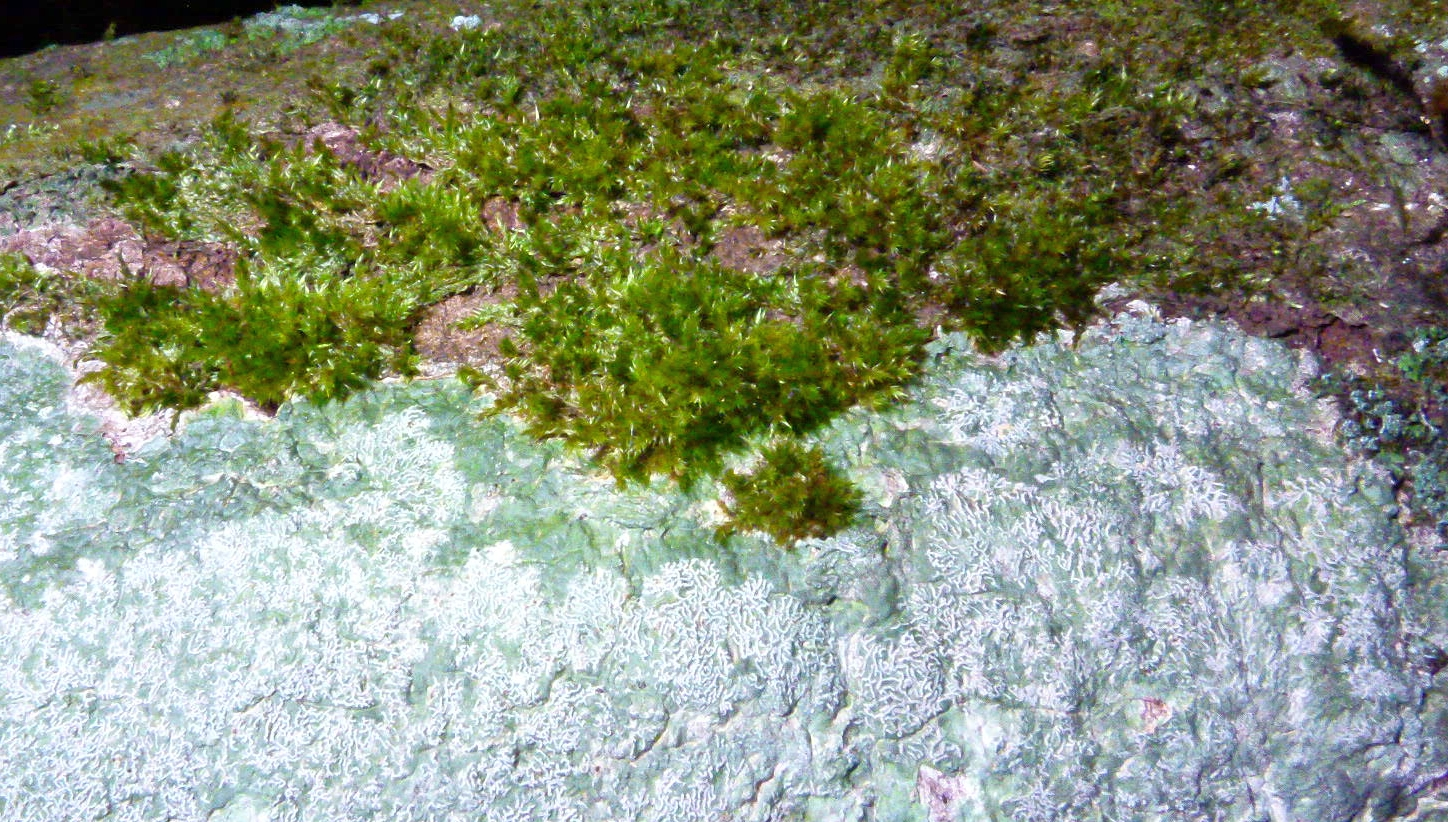
\includegraphics[width=0.45\linewidth]{./figs/lichen} 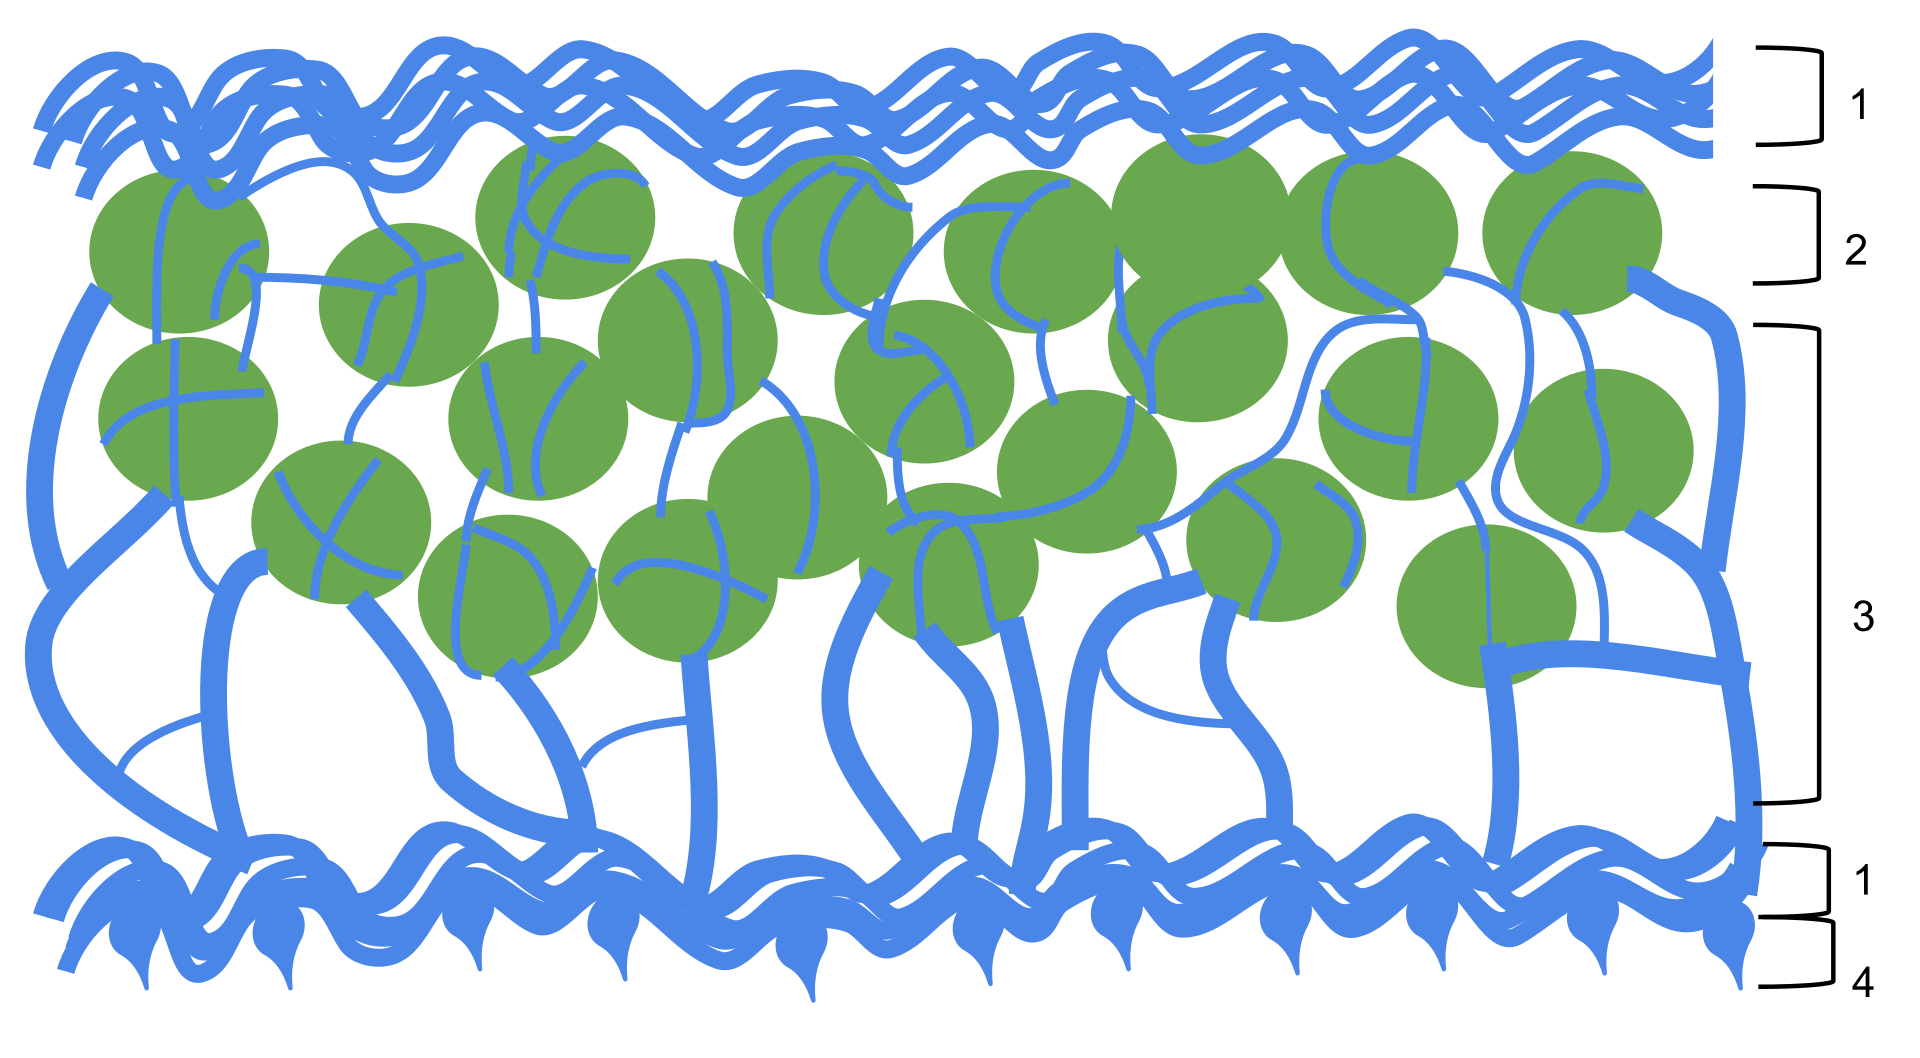
\includegraphics[width=0.45\linewidth]{./figs/LichenDiagram} 

}

\caption{Links: Korstmossen, een uniek organisme dat rotsen kan koloniseren (Bron: Shyamal, Wikipedia). Rechts: Korstmossen zijn een symbiose van een groene alg en een schimmel. 1. Dikke lagen schimmeldraden die de groene alg beschermen 2. Groenalgen 3. Los opeengepakte schimmeldraden 4. Verankerende schimmeldraden die als een soort wortels fungeren (Jdurant, Wikipedia).}\label{fig:lichen}
\end{figure}

Hoewel korstmossen macroscopisch op één wezen lijken, zijn het feitelijk twee wezens: een groene alg met de kostbare gave van fotosynthese die zonlicht en lucht in suikers verandert, en een schimmel die onderdak biedt en de kunst heeft om mineralen uit de rotsen te halen, maar die zelf geen suikers kan maken. Ze zijn verenigd in een symbiose die zo intens is dat ze samen een geheel nieuw organisme vormen. Toen biologen dit unieke huwelijk tussen algen en schimmels probeerden te ontrafelen, kweekten ze deze eerst in het laboratorium onder ideale omstandigheden. Onder deze omstandigheden bleven ze echter allebei gelukkig naast elkaar leven. De unieke eigenschappen van korstmossen konden dus niet worden afgeleid door beide soorten afzonderlijk te bestuderen. Pas toen de wetenschappers hen blootstelden aan barre ecofactoren, gingen ze opnieuw samenwerken en verkregen ze opnieuw hun unieke transformerende kracht om op rotsen te groeien en deze heel langzaam in een vruchtbare omgeving te veranderen \citep{Kimmerer2013}.

\hypertarget{leven-als-een-emergente-eigenschap}{%
\subsection{Leven als een Emergente Eigenschap}\label{leven-als-een-emergente-eigenschap}}

\citet{capraLuisi2014} argumenteren overtuigend dat hetzelfde geldt op elk niveau en dus ook voor het leven zelf. De autopoëtische eigenschap van een cel ontstaat doordat al zijn moleculen op de juiste manier worden gecombineerd in de grote netwerken van chemische reacties waaruit de structuur en organisatie, het zelfonderhoud en de zelfreplicatie spontaan ontstaan. We kunnen het leven niet lokaliseren. Het leven is eenvoudigweg een universele eigenschap die voortkomt uit de collectieve interacties van allerlei soorten moleculen in een cel, uit de verzameling cellen in een weefsel, uit de verzameling weefsels in een orgaansysteem, uit de verzameling orgaansystemen van een organisme, uit de verzameling organismen in een populatie, \ldots{} Op elk niveau hebben we een netwerk van componenten op een lager niveau waaruit op natuurlijke wijze nieuwe eigenschappen voortkomen.

Het leven zelf is dus een emergente eigenschap, het is niet aanwezig in de delen waaruit het voortkomt, en manifesteert zich pas als de delen op de juiste manier met elkaar worden geassembleerd.

\hypertarget{het-leven-als-gestalt-van-de-autopouxebtische-eenheid-cognitie-en-omgeving}{%
\subsection{Het Leven als Gestalt van de Autopoëtische Eenheid, Cognitie en Omgeving}\label{het-leven-als-gestalt-van-de-autopouxebtische-eenheid-cognitie-en-omgeving}}

Voor Maturana en Varela is cognitie ook onlosmakelijk verbonden met autopoësis \citep{capraLuisi2014}. Elk levend organisme is een open systeem dat via zijn sensorische arsenaal interageert met zijn omgeving. Het voelt zijn omgeving, het voedt zich met zijn omgeving, laat er producten in los, het verandert zijn omgeving en actualiseert zichzelf door de interacties met zijn omgeving. Het feit dat een organisme zijn omgeving verandert, wordt vaak over het hoofd gezien. Het biologische leven heeft de aarde echter dramatisch getransformeerd. Denk bijvoorbeeld aan de fotosynthese die de aarde radicaal veranderde door de massale uitstoot van het zeer reactieve molecule zuurstof.

Een organisme is op elk moment in zijn ontwikkeling een logboek van zijn eerdere interacties met zijn omgeving en dat bepaalt zijn toekomstige interacties. Cognitie is dus een natuurlijke eigenschap van zijn evolutie.

Varela ziet het leven als een gestalt van drie domeinen \citep{capraLuisi2014}:

\begin{itemize}
\tightlist
\item
  Omgeving,
\item
  Cognitie en
\item
  De autopoëtische eenheid.
\end{itemize}

Volgens hem is het leven de synergie van deze drie domeinen, die hij de ``embodied mind'' noemt.

\hypertarget{ons-sociale-systeem-als-een-emergente-eigenschap}{%
\subsection{Ons Sociale Systeem als een Emergente Eigenschap}\label{ons-sociale-systeem-als-een-emergente-eigenschap}}

De inzichten van Maturana en Varela impliceren dat we de dualiteit van materie en geest niet langer nodig hebben als we het leven proberen te begrijpen. Leven ontstaat op natuurlijke manier als een emergente eigenschap van de grote netwerken van materie of moleculen op het niveau van elke individuele cel, de fundamentele autopoietische eenheid. Vervolgens ontstaan er nieuwe eigenschappen op een hoger niveau wanneer autopoietische eenheden worden gecombineerd tot weefsels, organen, orgaansystemen en organismen, populaties, \ldots{}

We kunnen ons cognitieve bewustzijn dan ook zien als een emergente eigenschap van het netwerk van onze neuronen in onze hersenen als gevolg van de geschiedenis van onze interacties met onze omgeving. Bewustzijn is inderdaad een uitdrukking van het leven, het is belichaamd en pathologieën kunnen ontstaan wanneer mentale processen dissociëren van onze lichamelijke ervaringen. Onze ``embodied mind'' is inderdaad opmerkelijk. In onze arrogantie zijn we echter vaak blind voor de intelligentie van andere levensvormen. Niettemin zijn de unieke nieuwe functies en processen die ontstaan wanneer menselijke individuen netwerken vormen verbazingwekkend.

Op het niveau van het netwerk van mensen, manifesteert ons rijke psycho-socio-emotionele leefwereld zich. Als mens speelt ons leven zich niet alleen af in het fysieke domein, maar ook in het sociaal-symbolische domein, wat cruciaal is voor onze ontwikkeling. Ons gedrag in het fysieke domein wordt dus bepaald door de ``natuurwetten'', terwijl ons gedrag in het sociale domein wordt bepaald door regels van het sociale systeem zelf \citep{capraLuisi2014}. Bovendien toonde onderzoek in de sociale wetenschappen aan dat sociale netwerken dezelfde algemene principes vertonen als biologische netwerken. Als mens ontwikkelen we onszelf dus in een geheel met interne regels die worden gegenereerd door onze netwerken en hun grenzen, met name de fysieke grenzen in onze biologische netwerken en de culturele grenzen in onze sociale netwerken \citep{capraLuisi2014}.

\hypertarget{gedeelde-bio-logica-van-cellen-tot-sociale-systemen}{%
\subsection{Gedeelde ``Bio-logica'' van Cellen tot Sociale Systemen}\label{gedeelde-bio-logica-van-cellen-tot-sociale-systemen}}

Net als het biochemische systeem van een cel is ons sociale systeem een open systeem met sociale feedbacklussen. Elk sociaal systeem houdt zichzelf op een stabiele maar dynamische manier in stand, door nieuwe leden, materialen en ideeën in het systeem binnen te laten, en die te transformeren door de interne regels van de organisatie van het systeem \citep{capraLuisi2014}, wat leidt tot een soort ``sociale homeostase''. Soms kunnen deze nieuwe ideeën zo krachtig zijn dat ze het sociale systeem vanzelf transformeren, dat wil zeggen dat de ideeën het sociale systeem van attractor laten omschakelen. Op individueel niveau zijn de transformaties die het sociale systeem oplegt soms gelukzalig, maar ze kunnen ook trauma's veroorzaken. De observatie dat de `biologische logica' of het organisatiepatroon van een eenvoudige cel vergelijkbaar is met die van een hele sociale structuur, heeft grote implicaties.

Zoals \citet{Kimmerer2013} zo overtuigend naar voren brengt in haar boek ``Een vlecht van heilig gras'', nodigen deze inzichten ons ook uit om te leren van alle levensvormen die ons omringen. Het korstmosvoorbeeld kan ons leren over onze relaties en de samenleving. In de labo-omgeving, toen de omstandigheden voor beide organismen optimaal waren, hadden zowel de schimmel als de groene algen geen interactie. Pas toen de omgeving voor hen beiden extreem werd, bundelden ze hun krachten en namen hun unieke korstmosvorm aan waar ze nauw met elkaar interageren en verweven zijn. Een soortgelijke verstoring van onze sociale functie is te zien in onze moderne westerse samenleving, die wordt overspoeld door consumptiegoederen en die individualisme en eenzaamheid cultiveert.

Deze gedeelde biologische logica, van cellen tot aan ons sociaal-symbolische leefwereld, suggereert dus een fundamentele eenheid van het leven \citep{capraLuisi2014}. Het impliceert dat er een holistisch perspectief nodig is om de menselijke ontwikkeling te bestuderen, iets wat Rolando Toro diep omarmde toen hij zijn systeem van Biodanza ontwikkelde.

Deze bio-psycho-socio-emotionele invalshoek is buitengewoon interessant, maar valt buiten het bestek van deze monografie.

\hypertarget{links-met-het-vitaal-onbewuste}{%
\section{Links met het Vitaal Onbewuste}\label{links-met-het-vitaal-onbewuste}}

``Het leven is één''! Alle soorten zijn ontstaan uit dezelfde populatie van voorouderlijke cellen, ze gebruiken dezelfde chemie en hetzelfde coderingssysteem om hun genetische informatie op te slaan. De rijkdom aan levende soorten, met hun eigen zintuiglijke arsenaal, zijn allemaal ontstaan uit onze laatste universele gemeenschappelijke voorouder door evolutie als gevolg van de interacties met hun omgeving. Alle levensvormen hebben dezelfde overkoepelende instincten. De expressie van deze overkoepelende instincten is echter anders gedifferentieerd en dat naar gelang de leefwereld van het organisme\footnote{Overkoepelende instincten: de uitdrukking van het vecht- en vluchtinstinct is bijvoorbeeld gedifferentieerd tot doornige structuren in planten, de indrukwekkende elegante vlucht van een gazelle met snelheden tot 100 km/u, en mensen die autorijden gaan op hun rem staan wanneer de remlichten van hun voorligger plots aangaan}. We voelen dus aan dat alle levende wezens nauw met elkaar verbonden zijn. Bovendien volgen de emergente eigenschappen van netwerken van levende wezens dezelfde ``biologische logica'' en suggereren ze een fundamentele eenheid van leven.

De cellen van levende organismen reageren op interne en externe stimuli door biochemische moleculen, eiwitten, hormonen en neurotransmitters te produceren. Die zijn de biochemische vertaling van de gedifferentieerde expressie van hun instincten. Ze bepalen hun reactie en hoe ze op elkaar inwerken in hun populatie. Onze reactie op ecofactoren in het milieu wordt grotendeels bepaald door onze ``embodied mind''. Die komt voort uit de verschillende niveaus van de autopoietische eenheden waaruit ons organisme bestaat, samen met de geschiedenis van de interacties met onze omgeving en sociale netwerken van onszelf, van onze voorouders en van de soorten waaruit we zijn voortgekomen.

Deze intieme verbinding met het leven dat één is, via onze ``embodied mind'', is naar mijn mening waar Rolando op doelde met de term \emph{vitaal onbewuste}.

Het is dus duidelijk dat alle biologische organismen dezelfde gemeenschappelijke overkoepelende instincten delen en dus een soort gemeenschappelijke cognitie hebben, en dit van ecosysteem, populatie, organisme, weefsel tot op cellulair niveau. Dat laatste noemde Rolando ook wel een soort \emph{cellulair psychisme}: met een geheugen en een vermogen tot affiniteit, afstoting, solidariteit en communicatie, evenals de herkenning van soortgelijke autopoietische structuren in andere levensvormen.

Dit gedeelde psychisme of vitaal onbewuste omvat dus de oorsprong van onze instincten, lichamelijke gewaarwordingen en diepere kennis die we onmiddellijk vanuit onze ``embodied mind'' kunnen ervaren. Vivencia is een pad om diep met het vitaal onbewuste te verbinden, om het te versterken en te herbalanceren, en dit langs de vijf lijnen van Biodanza.

\hypertarget{rolando-toros-visie-op-het-leven}{%
\section{Rolando Toro's Visie op het Leven}\label{rolando-toros-visie-op-het-leven}}

Nu we een dieper inzicht hebben verworven over de principes van het leven, kunnen we Rolando Toro's visie op het leven beter begrijpen.
Rolando Toro reduceert leven niet tot het biologische leven.
Voor hem is leven het organiserende principe van het universum.
Vandaar zijn quote: ``leven is de essentiële voorwaarde voor het ontstaan van het universum''.

Pas aan het einde van de monografie werd het voor mij duidelijk dat Rolando zijn visie op leven expliciet heeft opgenomen in het Model van Biodanza. Al die tijd al, stond het daar, gewoon voor mijn neus: ``Principi di vita cosmica Anabasi'' en ``Principi di vita cosmica Catabasi''.
Leven bestaat uit de twee drijvende krachten anabasis en katabasis die aan de oorsprong liggen van alle structuur en dus van leven in het universum.

Die krachten vinden we op elke schaal terug.
Op de schaal van het volledige universum kan de oerknal als een groot katabasis event worden gezien. Een enorme vernietiging van iets die onmiddellijk de nucleus in zich droeg van nieuw leven in ons universum. Na die initiële flits van ontstaan, volgde de anabasis of de opbouw van alle rijkdom en structuur die we rondom ons waar kunnen nemen.\\
En als we elk van die structuren bestuderen zien we dat ze ook weer zijn ontstaan uit de pulsatie tussen Katabasis en Anabasis. Een pulsatie tussen respectievelijk vernietiging die de kiem van nieuw leven in zich draagt en de opbouw van structuur.

In tegenstelling tot Varella en Maturana die leven zien als een emergente eigenschap, als een gestalt van omgeving, een autopoëtische eenheid en cognitie, ziet Rolando het leven dus als het organiserende principe van het universum. Uitgedrukt in de taal van Varella en Maturana, ontwikkelen de twee creatieve krachten van het leven volgens Rolando dus een steeds evoluerende gestalt van omgeving, autopoëtische eenheden en cognitie.
Bovendien is leven voor Rolando nog veel alomvattender. Hij beperkt zich niet tot biologische leven waarin autopoëtische eenheden zijn betrokken. Alle structuren in het universum komen voor hem door het leven tot stand. ``Het leven is één'', één grote kosmische dans, of om het met Rolando's woorden te zeggen ``het rijk van het leven omvat veel meer dan de planten, de dieren en de mens. Alles wat bestaat, van neutrino's tot quasars, van edelsteen tot de meest subtiele gedachte, maakt deel uit van dit wonderbaarlijke levende systeem.''

Nu we een goed begrip hebben van Rolando's kijk op leven, zullen we in de volgende hoofdstukken dieper ingaan op waar, hoe en waarom de biologische aspecten voorkomen in het Biodanza-Model. Merk wel op dat veel van de concepten die we vanuit biologisch perspectief zullen bespreken ook een belangrijke sociologische, psychologische, emotionele en mystieke dimensie hebben, aangezien een groot deel van ons menselijk leven zich afspeelt in het sociaal-symbolisch domein.

\hypertarget{principes-van-het-kosmische-leven-en-de-genese-van-het-leven}{%
\chapter{Principes van het Kosmische Leven en de Genese van het Leven}\label{principes-van-het-kosmische-leven-en-de-genese-van-het-leven}}

De biologische aspecten vormen de verticale as van het Biodanza-Model. Onderaan het model komen we eerst de Principes van Kosmisch Leven en de Genese van het Leven tegen, die in Figuur \ref{fig:modelCosmic} zijn aangeduid met het rode kader.

\begin{figure}

{\centering 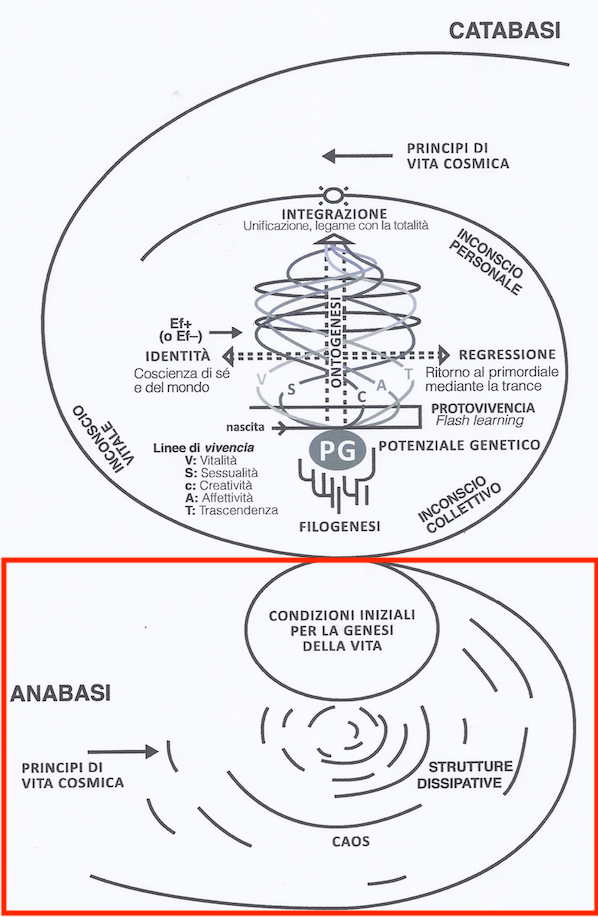
\includegraphics[width=0.5\linewidth]{./figs/biologischeAspectenBiodanzaDeelI} 

}

\caption{Biodanza-Model met aanduiding van de Principes van het Kosmische Leven en de Genese van het Leven}\label{fig:modelCosmic}
\end{figure}

We beginnen met het ontstaan van het universum en eindigen met het ontstaan van het biologische leven. Deze twee secties behandelen concepten uit de reader voor ``Module IV: Biologische aspecten van Biodanza''.

\hypertarget{ontstaan-van-het-universum}{%
\section{Ontstaan van het Universum}\label{ontstaan-van-het-universum}}

Figuur \ref{fig:evolutionUniverse} geeft een overzicht van de evolutie van het heelal.

\begin{figure}

{\centering 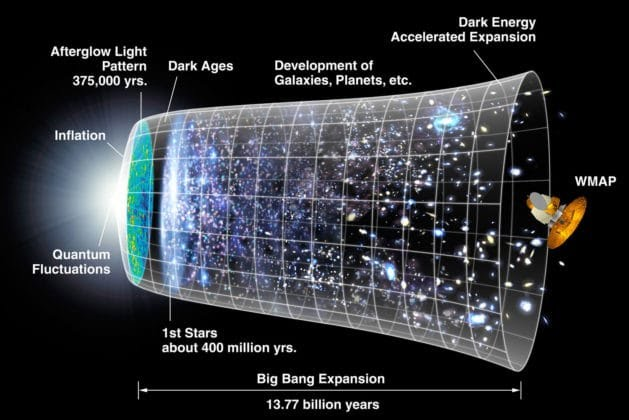
\includegraphics[width=1\linewidth]{./figs/originKosmos} 

}

\caption{Ontstaan ​​en evolutie van ons heelal (Bron: NASA/WMAP Science Team, Wikipedia)}\label{fig:evolutionUniverse}
\end{figure}

De meest gangbare theorie is dat onze kosmos begon met de oerknal. Een zeer energierijke staat.

Door de uitdijing koelde het heelal af waardoor een deel van de energie werd omgezet in waterstof en een fractie in zwaardere heliumkernen.

\hypertarget{ontstaan-van-de-sterren}{%
\subsection{Ontstaan van de Sterren}\label{ontstaan-van-de-sterren}}

Onder invloed van de zwaartekracht begon de materie zich vervolgens te clusteren in nevels, gaswolken die hoofdzakelijk uit waterstof (H) en helium (He) bestonden.

Als gevolg van concentratieverschillen in deze eerste nevel trokken deze wolken zich verder samen en implodeerden ze uiteindelijk (zie Figuur \ref{fig:genesisStar}).

\begin{figure}

{\centering 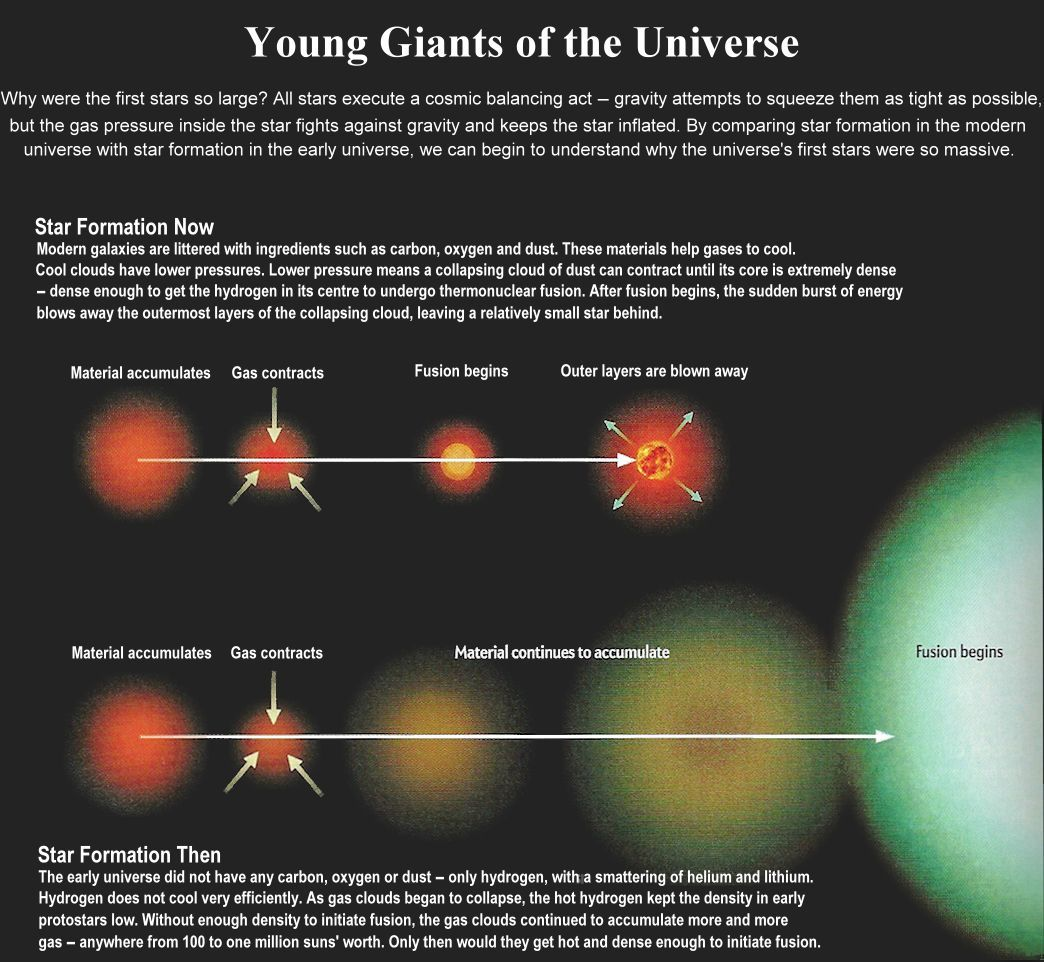
\includegraphics[width=1\linewidth]{./figs/I08-13-firststars6} 

}

\caption{Onstaan van de eerste sterren (Bron: universe-review.ca)}\label{fig:genesisStar}
\end{figure}

Extreme verhitting in de nevel die door de zwaartekracht implodeerde, leidde tot een toestand waarin alle materie de vorm had van een superheet plasma. In zo'n plasma vindt spontaan kernfusie plaats. Bij dit proces worden lichte atomen gecombineerd tot zwaardere atomen en komt er veel energie vrij.

Eerst worden alle waterstofatomen omgezet in helium (zie Figuur \ref{fig:nuclearFusion}). De massa van de resulterende heliumkernen is iets lager dan die van de oorspronkelijke waterstofkernen en het massaverschil wordt omgezet in energie.

\begin{figure}

{\centering \includegraphics[width=0.5\linewidth]{./figs/fusion} 

}

\caption{Kernfusie van waterstof tot het zwaardere helium (Bron: Sarang, Wikipedia)}\label{fig:nuclearFusion}
\end{figure}

Als alle waterstof in een ster is opgebruikt, stopt de fusie omdat de activeringsenergie om helium in lithium om te zetten te hoog is (Figuur \ref{fig:fusionEnergy}).

\begin{figure}

{\centering 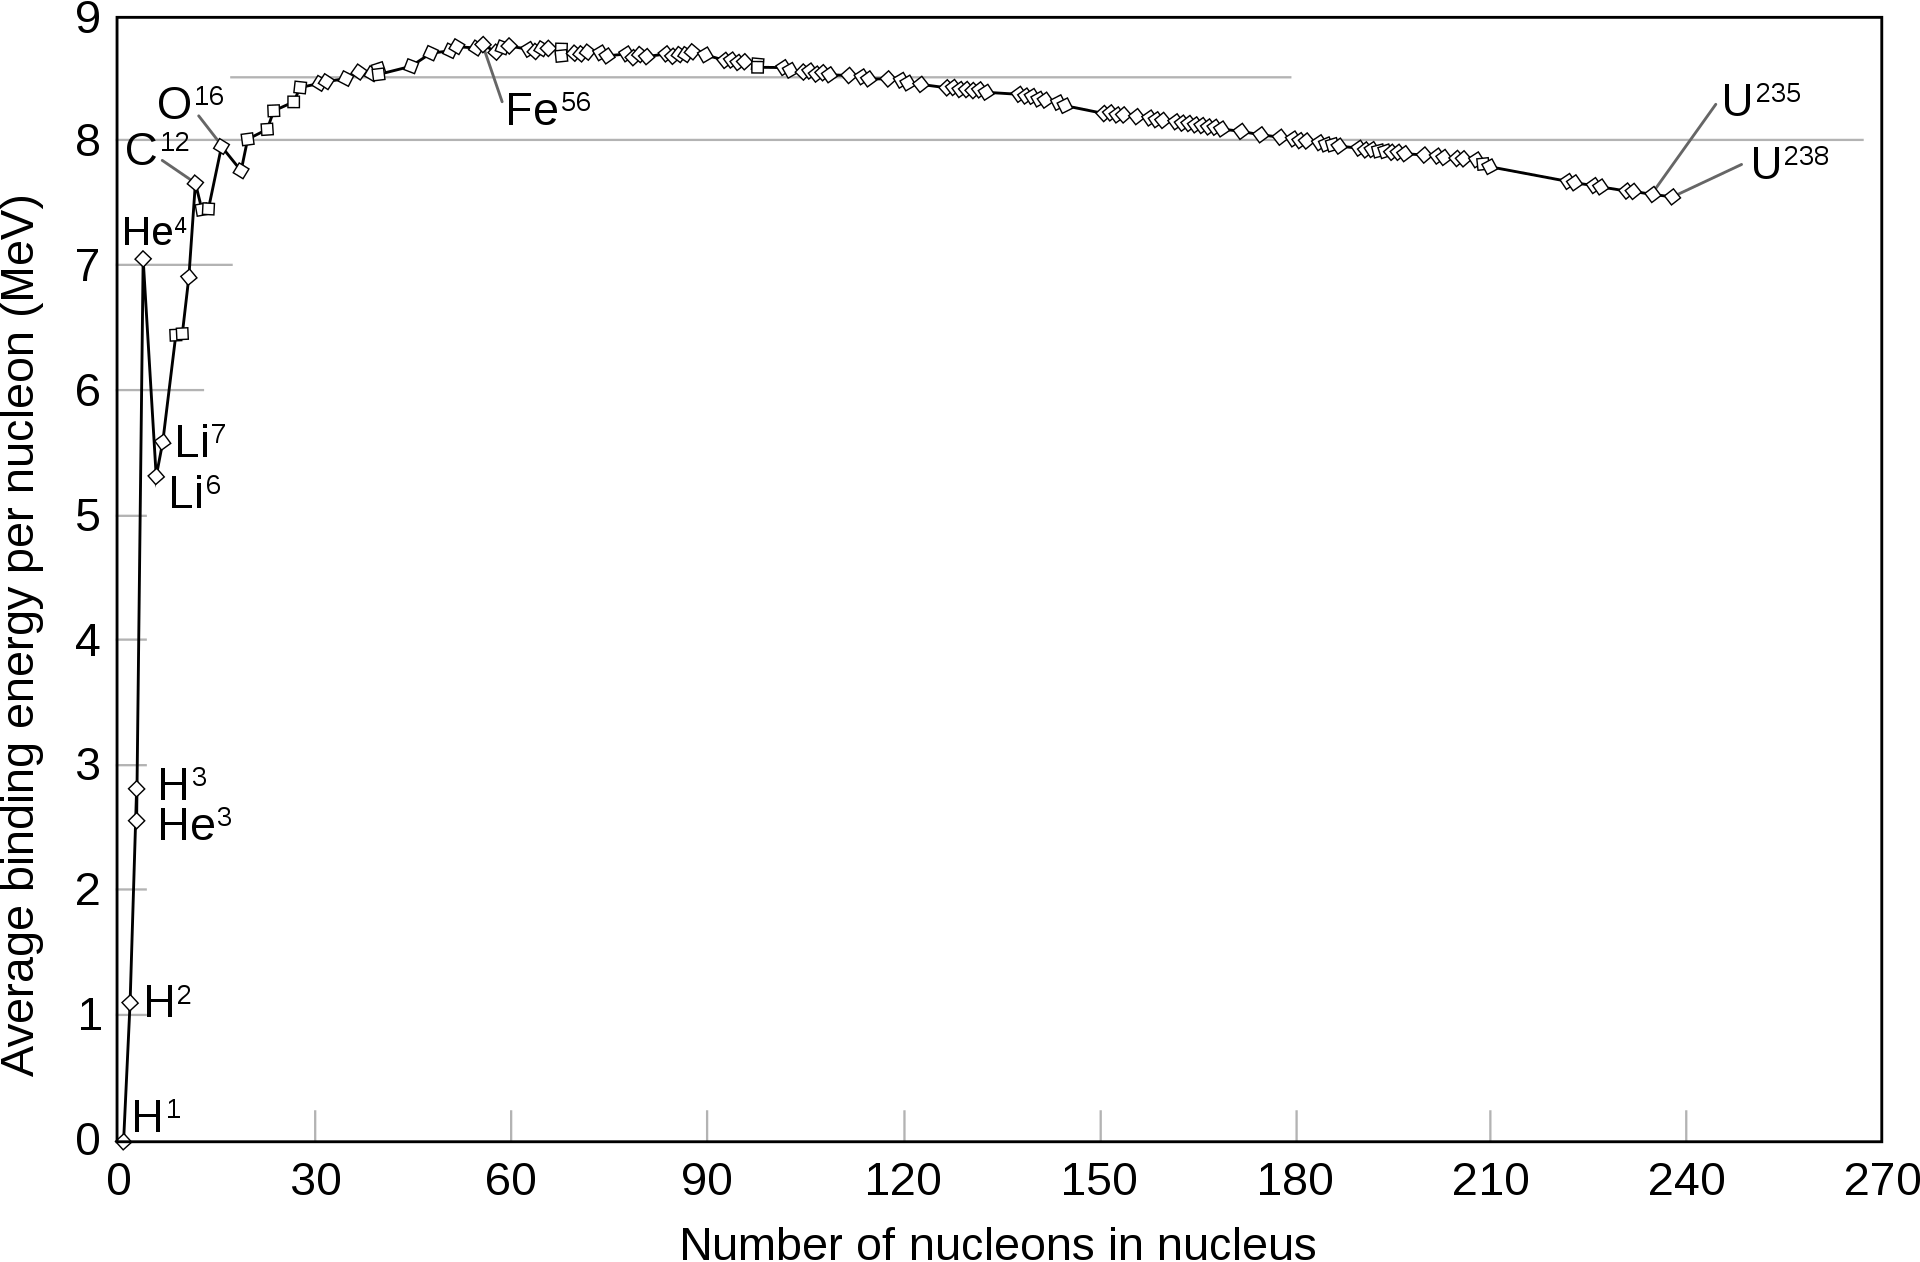
\includegraphics[width=0.5\linewidth]{./figs/fusionEnergy} 

}

\caption{Energie die vrijkomt door kernfusie. In een ster vindt kernfusie plaats tot ijzer (Bron Wikipedia)}\label{fig:fusionEnergy}
\end{figure}

Daarom koelt de ster af, implodeert ze waardoor het nog warmer wordt. Hierdoor kan de activatie energie van helium naar lithium worden overschreden en vindt spontaan kernfusie plaats van de zwaardere elementen tot ijzer (Figure \ref{fig:fusionEnergy}). Er komt hierbij zoveel energie vrij dat de ster explodeert tot een supernova (zie Figuur \ref{fig:supernova}). Tijdens de supernova worden deze nieuw gevormde elementen in het universum geslingerd.

\begin{figure}

{\centering 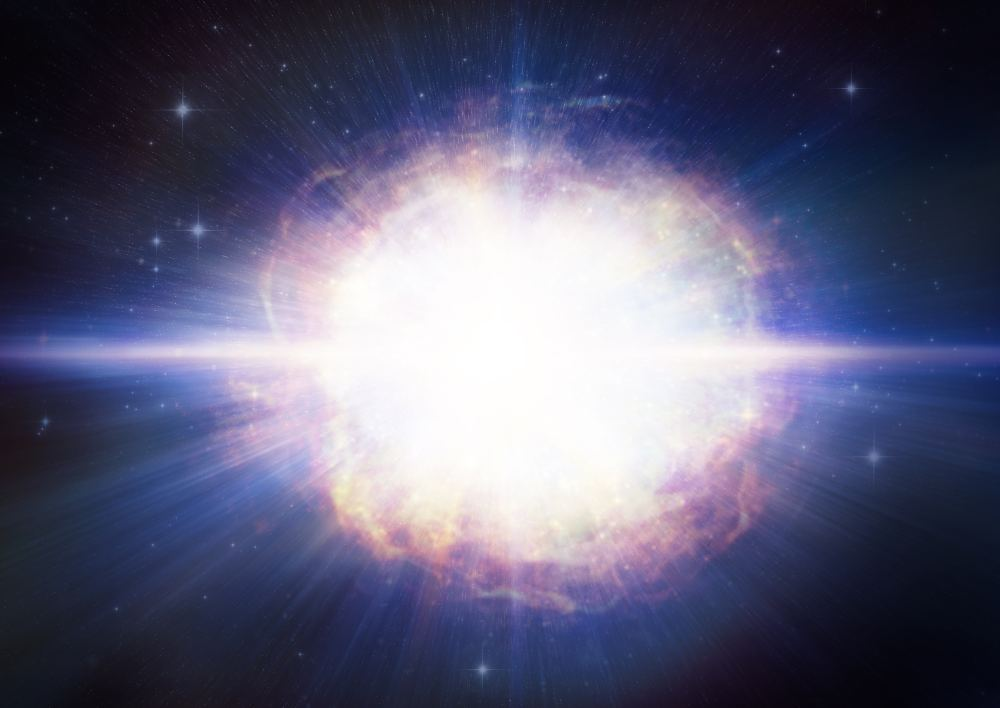
\includegraphics[width=0.5\linewidth]{./figs/hires} 

}

\caption{Supernova van een ster (Bron:  www.universetoday.com)}\label{fig:supernova}
\end{figure}

Uit supernova worden nieuwe nevels gevormd en deze zullen uiteindelijk leiden tot nieuwe sterren en het hele proces begint van vooraf aan.

Door kernfusie in de sterren zijn dus de zwaardere atomen ontstaan waaruit uiteindelijk de biomoleculen van het leven worden opgebouwd. Wij zijn dus opgebouwd uit sterrenstof!

\newpage

\hypertarget{koolhydraten-in-de-interstellaire-ruimte}{%
\subsection{Koolhydraten in de Interstellaire Ruimte}\label{koolhydraten-in-de-interstellaire-ruimte}}

Tijdens kernfusie in de sterren worden veel verschillende elementen gevormd. Voor biologisch leven zijn onder andere waterstof-, koolstof-, zuurstof-, zwavel-, fosfor- en stikstofatomen van cruciaal belang voor de samenstelling van organisch materiaal.

In de interstellaire ruimte reageert koolstof spontaan met andere elementen en vormt het poly-aromatische koolhydraten (PAK's). Die zijn bijvoorbeeld zichtbaar op een foto van de Cat's Paw nebula (Figuur \ref{fig:catPawNebula}). Het groene licht in de foto, is het gevolg van straling van hete sterren die fluorescentie van PAK's induceert.

\begin{figure}

{\centering 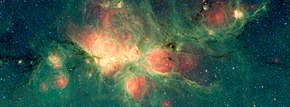
\includegraphics[width=0.5\linewidth]{./figs/orionWithPAH} 

}

\caption{Cats Paw nebula, de groene gebieden zijn het gevolg van straling van hete sterren die fluorescentie van PAKs induceert. (Source: NASA/JPL-Caltech, Wikipedia)}\label{fig:catPawNebula}
\end{figure}

PAK's ontstonden al kort na de oerknal. Zodra ze zijn geproduceerd, worden ze verder getransformeerd in de interstellaire ruimte door reactie met onder meer waterstof en zuurstof, om precursormoleculen (``voorlopers'') te vormen voor aminozuren en nucleotiden, die de respectievelijke bouwstenen zijn van eiwitten, en van RNA en DNA. Deze bouwstenen zijn essentieel voor de chemie van het leven en zijn dus al alomtegenwoordig in de ruimte.

Dit, naast andere argumenten, was voor Christian de Duve de aanleiding voor zijn citaat: ``Life is an obligatory manifestation of matter, written into the fabric of the universe'' \citep{deDuve2002}.

\hypertarget{ontstaan-van-het-leven}{%
\section{Ontstaan van het leven}\label{ontstaan-van-het-leven}}

In een uithoek van onze Melkweg, wat een modaal sterrenstelsel is, werd een modale planeet gevormd, die wij kennen als onze planeet Aarde. Nadat de aarde was afgekoeld, ontstond er vloeibaar water. De unieke eigenschappen van vloeibaar water zijn essentieel voor het biologische leven zoals wij dat kennen. Toen er eenmaal vloeibaar water beschikbaar was, ontstond het biologische leven in minder dan 300 miljoen jaar, wat een zeer kort tijdsinterval is op de geologische tijdschaal.

Zo waren er op aarde omstandigheden die het ontstaan van het biologische leven, zoals wij dat kennen, mogelijk maakten. Het exacte proces dat tot biologisch leven op aarde heeft geleid is niet gekend en dat zal waarschijnlijk zo blijven. Een algemene redenering wordt echter weergegeven in figuur \ref{fig:originOfLife}.

\begin{figure}

{\centering 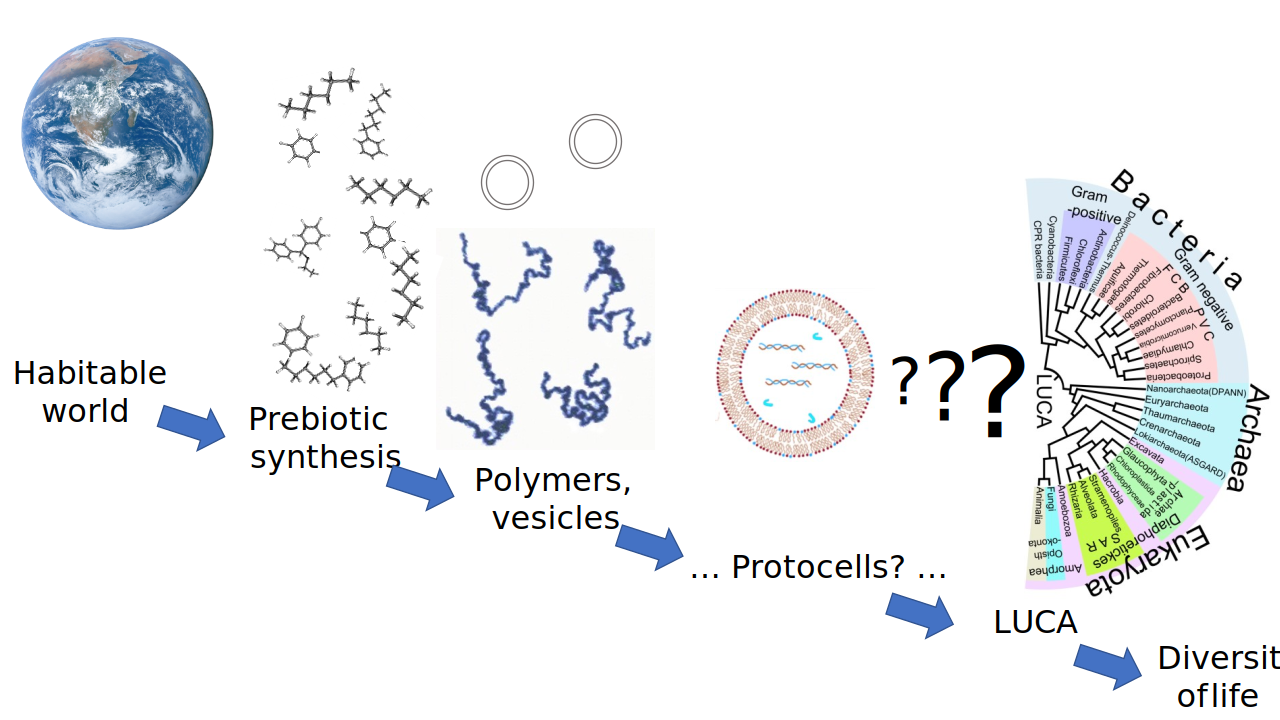
\includegraphics[width=1\linewidth]{./figs/origin_of_life_stages} 

}

\caption{Stadia in de oorsprong van het leven variëren van goed begrepen, zoals de abiotische synthese van eenvoudige organische moleculen, tot grotendeels onbekend, zoals de oorsprong van de laatste universele gemeenschappelijke voorouder (LUCA) met zijn complexe moleculaire functionaliteit. (Bron: Chiswick Chap, Wikipedia)}\label{fig:originOfLife}
\end{figure}

Eerst was er een chemisch evolutieproces die aan de basis lag van het ontstaan van organische moleculen met toenemende complexiteit. Het is een algemene consensus dat RNA-moleculen het eerst uit vrije nucleotiden voortkwamen. RNA-moleculen kunnen zowel katalytisch zijn alsook dragers van genetische informatie. Ze kunnen zichzelf ook vermenigvuldigen onder anoxische omstandigheden (in afwezigheid van zuurstof) en in aanwezigheid van ijzer, omstandigheden zoals op de jonge planeet Aarde (b.v. \citet{Williams2013}). Deze RNA-moleculen evolueerden ofwel alleen, volgens de RNA-wereldhypothese, ofwel al in combinatie met eiwitten.

Vervolgens wordt aangenomen dat prebiotische moleculen, die zichzelf konden vermenigvuldigen, werden ingekapseld door fosfolipiden, die spontaan membraanachtige structuren vormen. Dit resulteerde in een protocel met een membraan (zie Figuur \ref{fig:originOfLife}).
In deze protocellen was een verdere chemische evolutie mogelijk en dat gescheiden van de omgeving. Die evolutie leidde uiteindelijk tot een zelfreplicerende en zelforganiserende cel die was opgebouwd uit de vier essentiële soorten biomoleculen van het biologische leven: lipiden, koolhydraten, eiwitten en nucleïnezuren.

Verdere biologische evolutie van deze eerste levende cellen leidde uiteindelijk tot onze laatste universele gemeenschappelijke voorouder (LUCA). LUCA moet minstens 355 genen hebben gehad, die alle levende organismen gemeen hebben. LUCA was anaëroob, leefde in de afwezigheid van zuurstof; behield zijn erfelijk materiaal met behulp van DNA, de genetische code; en - produceerde eiwitten uit RNA-sjablonen in ribosomen. LUCA haalde zijn energie uit oceanische vulkanische activiteit in diepzeeopeningen, de intens hete pluimen van zeewater dat in contact komt met magma dat door de oceaanbodem uitbarst. En uiteindelijk evolueerde LUCA naar alle soorten die momenteel op aarde leven.

Nu we hebben stilgestaan bij het ontstaan van het leven, kunnen we ons concentreren op de fylogenes of het verhaal van de evolutie van LUCA tot alle soorten van de levensboom.

\hypertarget{fylogenese-en-evolutie}{%
\chapter{Fylogenese en Evolutie}\label{fylogenese-en-evolutie}}

In het midden van het Biodanza-Model in Figuur \ref{fig:modelPhylo} zien we het Biologisch Aspect ``fylogenese'' aangeduid in het rode kader.

\begin{figure}

{\centering 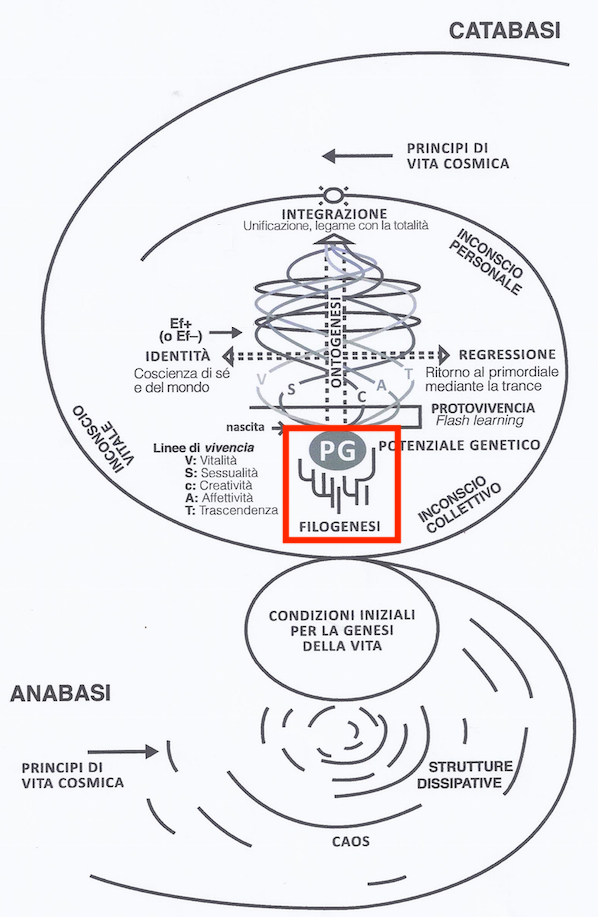
\includegraphics[width=0.5\linewidth]{./figs/biologischeAspectenBiodanzaDeelII} 

}

\caption{Model of Biodanza and Phylogenesis}\label{fig:modelPhylo}
\end{figure}

Fylogenese is het biologische proces of evolutionaire mechanisme waardoor een soort of een groep soorten verschijnt. Dit concept was erg belangrijk voor Rolando Toro, omdat het laat zien hoe verwant alle biologische organismen zijn en hoe natuurlijk het is dat hun levens allemaal volgens dezelfde principes zijn gestructureerd.

Voor Rolando ging de evolutie verder dan de biologische evolutie. Volgens hem bestaat het leven in essentie uit twee belangrijke processen: Anabasis en Katabasis, waaruit alle structuren in het universum zijn ontstaan. Anabasis is de integratie van chaos naar zelforganiserende systemen, terwijl Katabasis verwijst naar de desintegratie van dergelijke systemen. Bij Katabasis onstaat echter onmiddellijk de kiem van nieuw leven.

Tijdens de evolutie van het heelal ontstonden er steeds complexere structuren. Dit impliceert echter niet dat de evolutie een richting heeft. Dat evolutie steeds van het ``eenvoudige'' naar het ``hogere of meer complexe'' gaat, is een wijdverspreide verwarring. In plaats daarvan kunnen we deze twee organisatieprincipes zien als een creatief proces dat leidt tot het genereren van nieuwe structuren; sommige zijn meer eenvoudig, terwijl andere complexer zijn; en ze hebben allemaal hun eigen ritme en unieke kosmische dans. Dus de essentie van evolutie is de rijkdom en diversiteit die ontstaat.

Volgens Rolando worden alle structuren in het universum gevormd door dezelfde principes: aantrekking en afstoting. De expressie van deze principes verschilt echter telkens dat een nieuwe structuur ontstaat en ze varieert ook in complexiteit. Aantrekking en afstoting kunnen inderdaad worden waargenomen vanaf een eenvoudig atoom tot op het niveau van sterrenstelsels; en bij biologische levensvormen zijn aantrekking en afstoting verder gedifferentieerd in

\begin{itemize}
\tightlist
\item
  positieve and negatieve fototaxis\footnote{Fototaxis: beweging en/of groei naar of weg van licht}, geotaxis\footnote{Geotaxis: beweging en/of groei als reactie op een zwaartekrachtveld} en chemotaxis\footnote{Chemotaxis: beweging en/of groei naar of weg van een chemische of biochemische concentratiegradiënt},
\item
  reflexen, eenvoudige reacties op stimuli
\item
  instincten,
\item
  emoties, tot
\item
  gevoelens.
\end{itemize}

Dat alles is essentieel voor ons om in homeostase\footnote{Homeostase: zelfregulerend proces waardoor een organisme de neiging heeft zijn stabiliteit en intern evenwicht in zijn steeds veranderende omgeving te behouden} te kunnen blijven terwijl we ons aanpassen aan omstandigheden die het beste zijn voor onze overleving.

Interessant is dat \citet{margulis1999} zei dat ``metaboliserende oerbacteriën zo efficient waren in het opnieuw maken van zichzelf (\ldots) dat het binnenste van onze cellen vandaag de dag chemisch gezien meer verwant is aan de externe omgeving van de vroege aarde, waarin het biologische leven ontstond, dan dat ze lijken op onze huidige zuurstofrijke wereld. Het leven is inderdaad sinds het begin en zonder enige discontinuïteit chemisch verbonden geweest met zijn verleden''. \citet{margulis1999} gaat verder dat ``het metabolische geheugen van moderne cellen hoogstwaarschijnlijk dateert van vóór de meeste oude gesteenten''. Het geheugen kan dus worden gezien als een intrinsieke eigenschap van biologische systemen en hun metabolische arsenaal is een weerspiegeling van de omgevingen waaraan ze zijn blootgesteld tijdens hun evolutionaire traject.

Volgens Rolando is de differentiatie van autonomie een ander belangrijk aspect van de evolutie. Autonomie geeft een organisme het vermogen om te reageren, om homeostase te handhaven, en dus het vermogen om te integreren met zijn externe omgeving zonder zijn identiteit te verliezen. De differentiatie van autonomie wordt weerspiegeld in de differentiatie van het (a) sensorisch-motorische, (b) immuun- en (c) cognitieve en communicatieve arsenaal van een organisme, waardoor het respectievelijk (a) de plasticiteit krijgt om zich aan te passen, (b) het vermogen heeft om zijn biologische integriteit te behouden door te herkennen wat endogeen\footnote{Endogeen: eigen} en vreemd is, en (c) het vermogen heeft om andere leden van zijn eigen soort te herkennen en ermee om te gaan. Deze drie belangrijke functies werden al vervuld door een aantal verschillende groepen eiwitten in bacteriën en evolueerden naar totaal aparte en complexe systemen in planten en dieren.

Daarom is het uiterst waardevol om te bestuderen wat alle biologisch leven gemeen heeft, zodat we onszelf beter kunnen begrijpen en ons (opnieuw) verbonden en verenigd kunnen voelen met het biologische leven en het hele universum.

We beginnen dit hoofdstuk met twee secties die meer technisch zijn en zich richten op de concepten gerelateerd aan Fylogenese en Evolutie zoals geïntroduceerd in de reader van de Biodanza lerarenopleiding ``Module IV: Biologische aspecten van Biodanza''. We sluiten dit hoofdstuk af met een meer filosofisch gedeelte over evolutie, de mensheid en Biodanza.

\hypertarget{fylogenese}{%
\section{Fylogenese}\label{fylogenese}}

Alle soorten zijn voortgekomen uit dezelfde voorouderlijke populatie van cellen. Dit wordt ook wel dezelfde Last Universal Common Ancestor (LUCA) genoemd. In de levensboom worden de evolutionaire relaties tussen verschillende organismen (en groepen van organismen) samengevat. Alle levende wezens zijn uiteindelijk terug te voeren op LUCA die zich aan de wortel van de boom bevindt, zie Figuur \ref{fig:treeOfLifeBis}.

\begin{figure}

{\centering 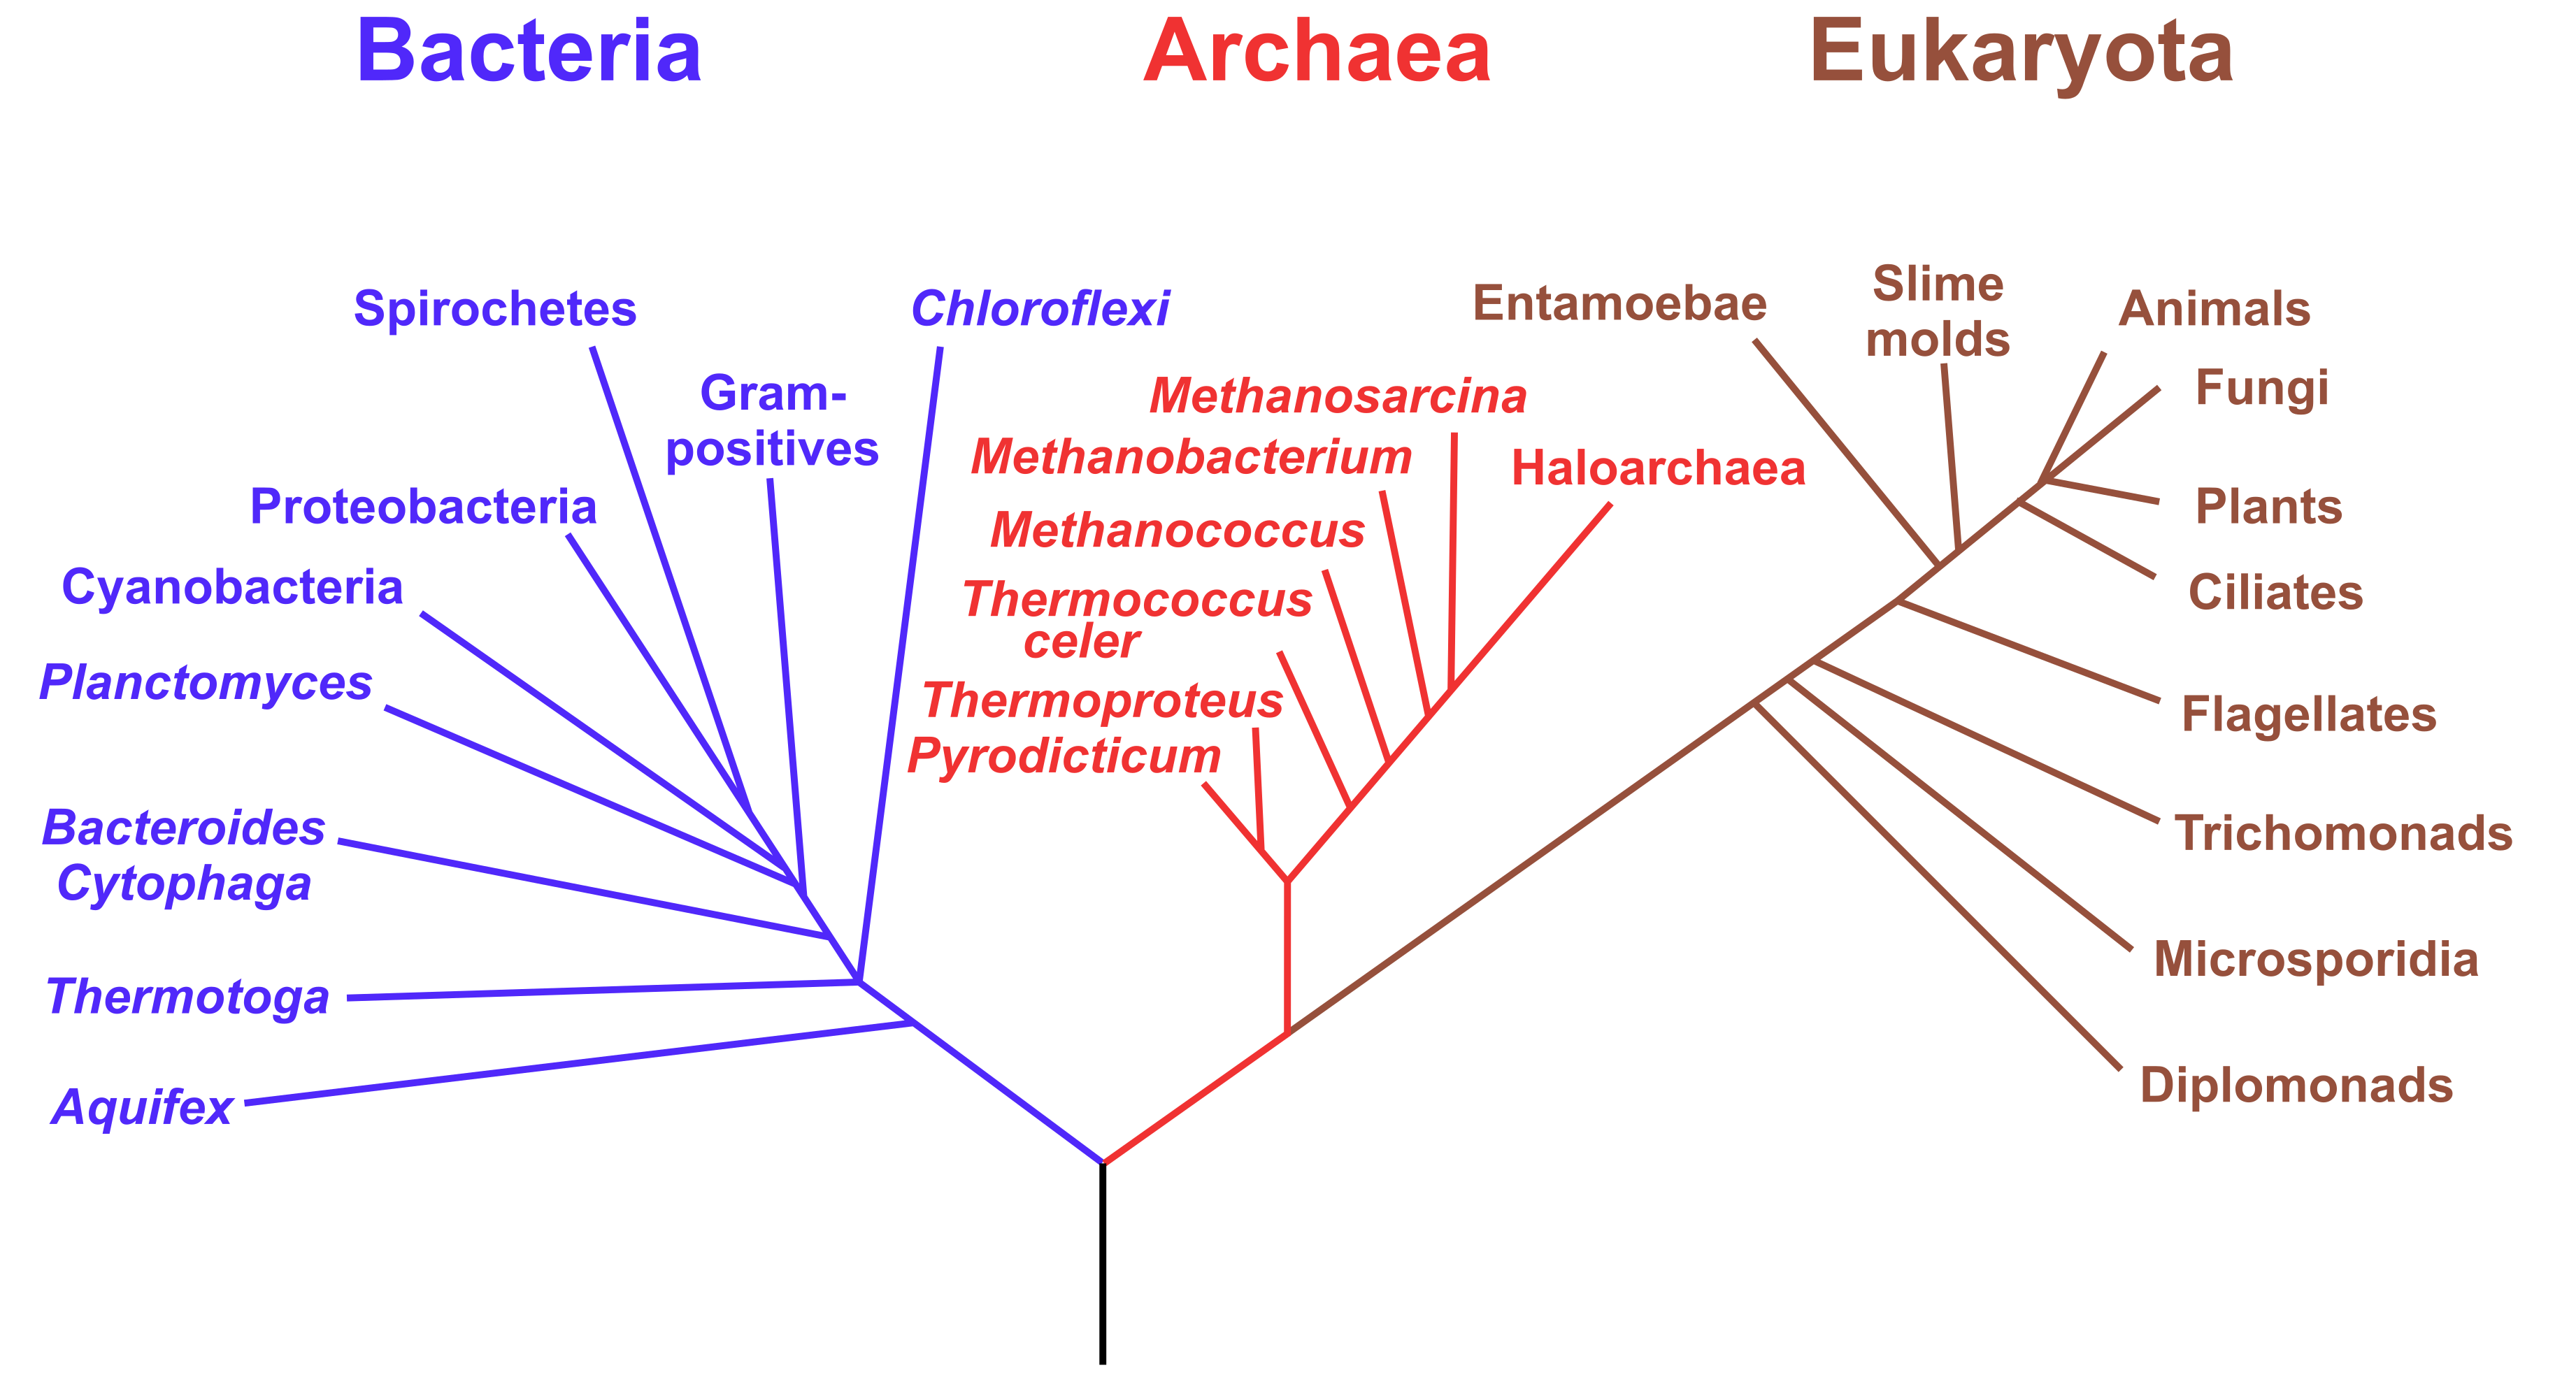
\includegraphics[width=1\linewidth]{./figs/Phylogenetic_tree} 

}

\caption{We hernemen hier de figuur van de levensboom. Het is één van de meest belangrijke organiserende principes in de biologie. Het toont de evolutionaire relaties tussen verschillende organismen en dat alle levende wezens uiteindelijk terug te voeren zijn op de laatste universele gemeenschappelijke voorouder die zich aan de wortel van de boom bevindt (Bron: wikipedia)}\label{fig:treeOfLifeBis}
\end{figure}

Fylogenese is het proces van het ontstaan van alle soorten uit de levensboom vertrekkende van LUCA.

Rolando Toro noemt de oorsprong van soorten en aanpassing aan de omgeving evolutionaire differentiatie. Hij beschouwt de genetische informatie van een soort als een logboek van de omgevingen en evolutionaire ontwikkeling die het tot nu toe heeft ondergaan.

\hypertarget{tijdschaal}{%
\subsection{Tijdschaal}\label{tijdschaal}}

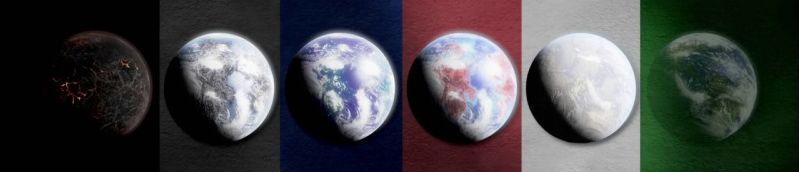
\includegraphics{./figs/liferockystartstrip.jpeg}

\begin{longtable}[]{@{}llllll@{}}
\toprule()
4.5 BYA & 4.3 BYA & 3.8 BYA & 3.5 BYA & 540 MYA & 520 MYA \\
\midrule()
\endhead
& & & & & \\
\bottomrule()
\end{longtable}

(Source: naturedocumetaries.org)

Bij haar oorsprong, ongeveer 4,5 miljard jaar geleden (BYA), was de aarde zwart, een hete basaltrots en stof in een koud vacuüm. Toen de aarde afkoelde, werd ze Grijze Aarde (4.3 BYA), omdat ze voornamelijk bedekt was met graniet en rotsen. Nog eens 500 miljoen jaar later was ze bedekt met vloeibaar water: Blauwe Aarde (3,8 BYA).

In slechts 300 miljoen jaar veranderde ze door het onstaan van biologische leven radicaal in Rode Aarde (3,5 BYA). Er zijn inderdaad cyanobacteriën ontstaan die aan fotosynthese kunnen doen en die massaal zuurstof zijn gaan produceren, een zeer reactief molecule. Dit leidde ertoe dat al het vrije ijzer in de oceaan neersloeg als ijzeroxide of roest (rood). Er vond een explosie plaats van het aantal mineraalsoorten. Hun aantal ging van ongeveer 250 naar ruim 5000 soorten. Zuurstof veroorzaakte ook een massale sterfte omdat slechts weinig organismen met het zeer reactieve karakter van zuurstof om konden gaan. De komende drie miljard jaar bleef het leven op aarde relatief gelijk.

Rond 540 MYA werd de aarde getroffen door een grote ijstijd, de Witte Aarde. Opnieuw leidde dit tot een massale uitsterving als gevolg van de kou. De vulkanische activiteit kwam echter te hulp door broeikasgassen te produceren en een atmosfeer te creëren die meer warmte vast kon houden.

In minder dan 20 miljoen jaar (MY) veranderde de aarde opnieuw radicaal in Groene Aarde (520 MYA). Er vond een explosie van leven plaats en het biologische leven evolueerde plotseling van voornamelijk eencellig naar complexe meercellige biologische levensvormen.

\hypertarget{evolutie}{%
\section{Evolutie}\label{evolutie}}

Hoe heeft de evolutie van LUCA naar alle soorten van de levensboom plaatsgevonden?

Lamarck (1744 - 1829) was een van de eerste voorgangers van biologische evolutie. Hij stelde de theorie voor dat (a) organismen hun gedrag veranderden als reactie op veranderingen in de omgeving, dat (b) hun veranderde gedrag op hun beurt hun organen veranderde, en dat (c) hun nakomelingen die `verbeterde' structuren erfden. Een theorie die is verlaten ten gunste van de evolutietheorie door natuurlijke selectie van Darwin (1809 - 1882) en Wallace (1823 - 1913). Voor hen bleven de mechanismen van reproductieve erfelijkheid en de oorsprong van nieuwe eigenschappen echter een mysterie. Bij de herontdekking van het werk van Mendel (1822 - 1884), die de basis legde voor populatiegenetica, werden natuurlijke selectie en populatiegenetica gecombineerd in de neodarwinistische theorie of de synthetische evolutietheorie. Sleutelprincipes in deze theorie zijn variabiliteit en selectie.

Het baanbrekende werk van Margulis (1938--2011) werpt echter een nieuw licht op de evolutie. Volgens haar theorie is symbiose een andere belangrijke motor van evolutie. Symbiose is een nauwe, langdurige associatie tussen twee of meer verschillende biologische soorten waarbij de betrokken soorten allemaal voordeel hebben van hun interactie. Vooral haar theorie van sequentiële endosymbiose, waarbij verschillende soorten bacteriën samensmolten om grotere en complexere cellen te vormen, kan de plotselinge explosie van levensvormen verklaren die werd waargenomen tussen 540 MYA en 520 MYA.

In deze paragraaf concentreren we ons eerst op de principes van variatie en selectie. We gaan dan verder met endosymbiose en symbiogenese. We sluiten dit deel af met een uitwerking van het concept teleonomie.

\hypertarget{variabiliteit-en-selectie}{%
\subsection{Variabiliteit en Selectie}\label{variabiliteit-en-selectie}}

Variatie ontstaat onder meer door fouten in het kopiëren van DNA voor de celdeling van prokaryotische cellen en de productie van gameten\footnote{Gameet: sperma- of eicel} voor eukaryotische cellen (zie Figuur \ref{fig:dnaPolymerase}).

\begin{figure}

{\centering 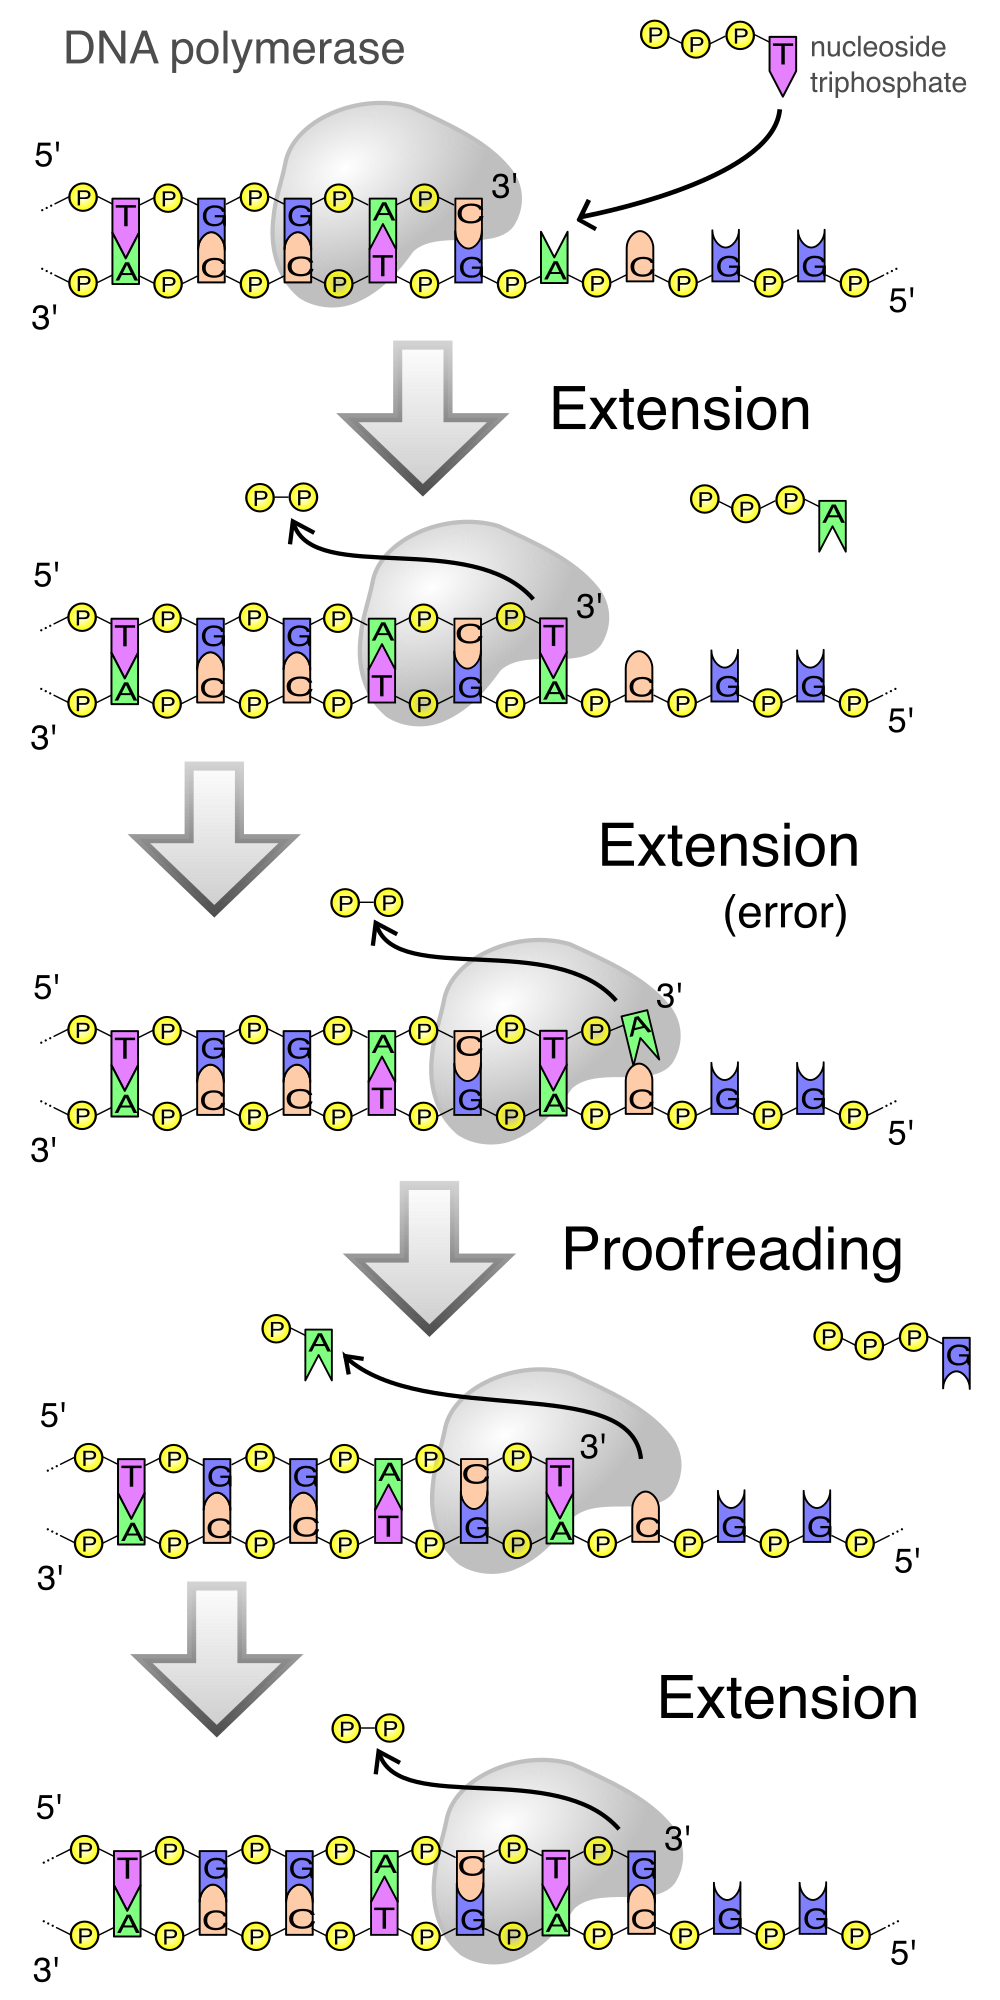
\includegraphics[width=0.45\linewidth]{./figs/DNA_polymerase} 

}

\caption{Kopiëren van DNA door DNA-polymerase. DNA-polymerase verlengt een DNA-streng door een complementair nucleoside-tri-fosfaat op te nemen en twee van de drie fosfaatgroepen te splitsen. Let opnieuw op het verband tussen energie en informatie. Fouten worden vaak gecorrigeerd door proeflezen. Sommige fouten blijven echter bestaan.}\label{fig:dnaPolymerase}
\end{figure}

De foutmarge bij DNA-replicatie bedraagt 1 fout per miljard basenparen die worden gekopieerd, wat tot puntmutaties kan leiden. Merk op dat wij mensen een genoomgrootte hebben van ongeveer 6,4 miljard basenparen.

Andere bronnen van variabiliteit zijn

\begin{itemize}
\tightlist
\item
  Inserties of deleties, dat wil zeggen basenparen die respectievelijk worden toegevoegd of verwijderd.
\item
  Recombinatie, herschikking van genetische eigenschappen, bijvoorbeeld tijdens seksuele voortplanting
\end{itemize}

De meeste mutaties zijn neutraal, dat wil zeggen dat het gemuteerde codon codeert voor hetzelfde aminozuur. Neutrale mutaties kunnen worden gebruikt als een moleculaire/genetische klok om te bepalen hoe ver twee soorten in evolutionaire zin van elkaar verwijderd zijn.

Maar mutaties zijn niet altijd neutraal! Sikkelcelanemie wordt bijvoorbeeld veroorzaakt door één puntmutatie in hemoglobine (zie Figuur \ref{fig:sickleCell1} en \ref{fig:sickleCell2}). Een T (thyminebase) wordt gemuteerd naar een A (adeninebase), wat resulteert in een codon dat codeert voor het aminozuur valine in plaats van glutaminezuur. Dit veroorzaakt drastische veranderingen in de 3D-structuur van het hemoglobine-eiwit en veroorzaakt een vervorming van de rode bloedcellen van een ronde naar sikkelvorm, wat leidt tot bloedarmoede.

Waarom blijft deze mutatie bestaan? Het komt vooral voor in Afrika, waar de mutatie voor sikkelcelanemie wordt geselecteerd omdat het de getroffen individuen resistent maakt tegen malaria. Dat geeft hen ondanks hun bloedarmoede toch een evolutionair concurrentievoordeel. Nakomelingen die de mutatie van beide ouders erven, zijn echter niet levensvatbaar. Daarom blijft ook de reguliere variant van hemoglobine bestaan.

\begin{figure}

{\centering 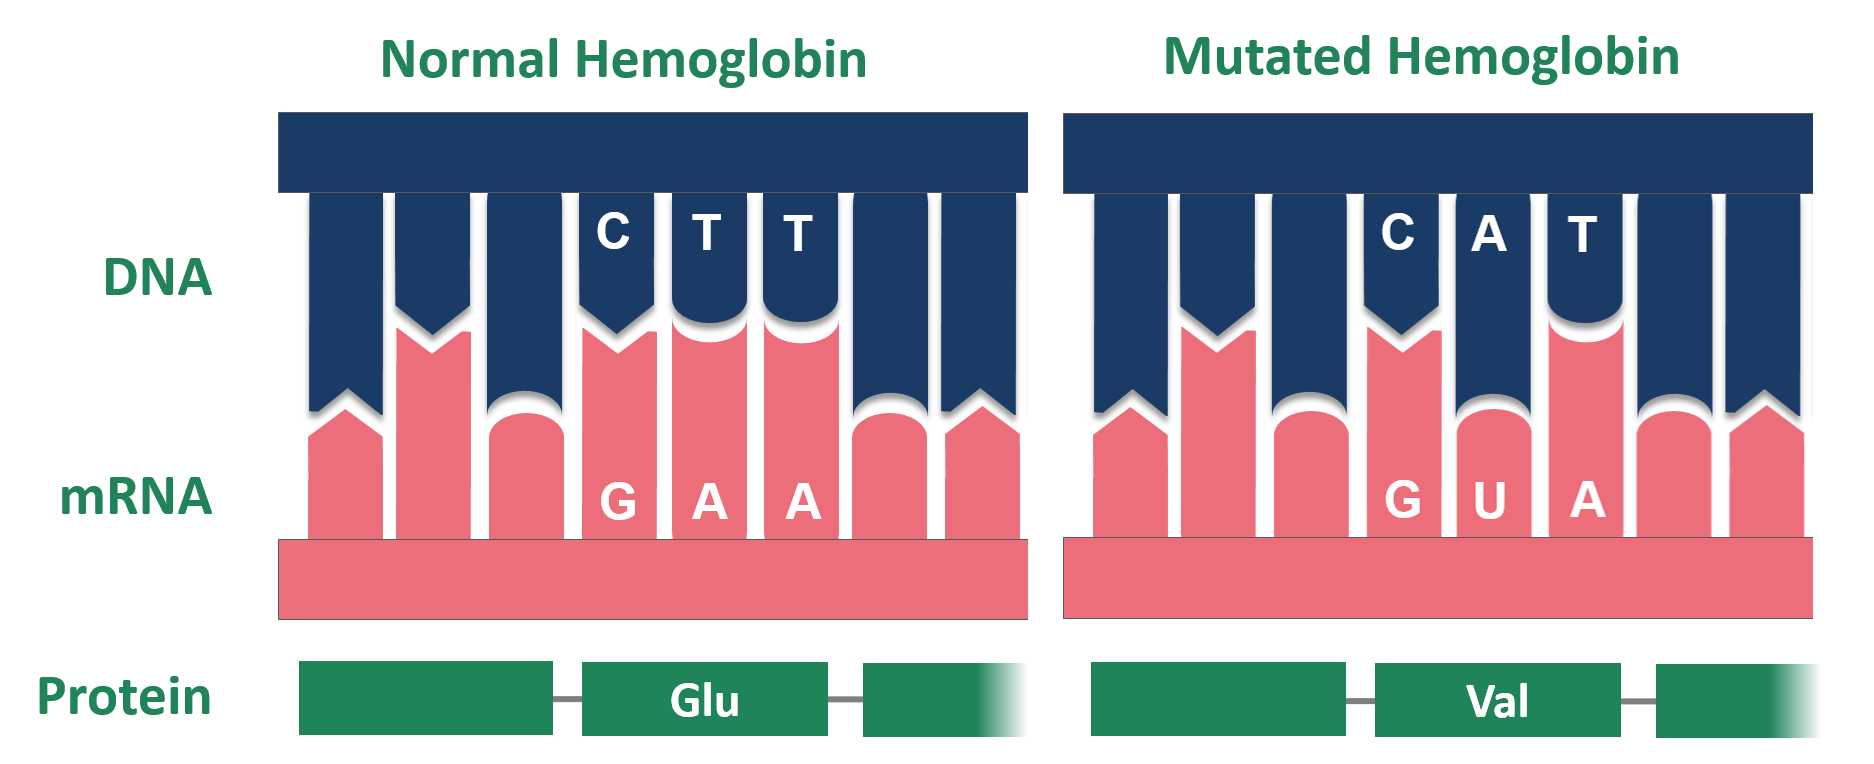
\includegraphics[width=0.45\linewidth]{./figs/sickleCellWikipedia2} 

}

\caption{Mutatie van hemoglobine bij patiënten met sikkelcelanemie (Bron: Wikipedia)}\label{fig:sickleCell1}
\end{figure}

\begin{figure}

{\centering 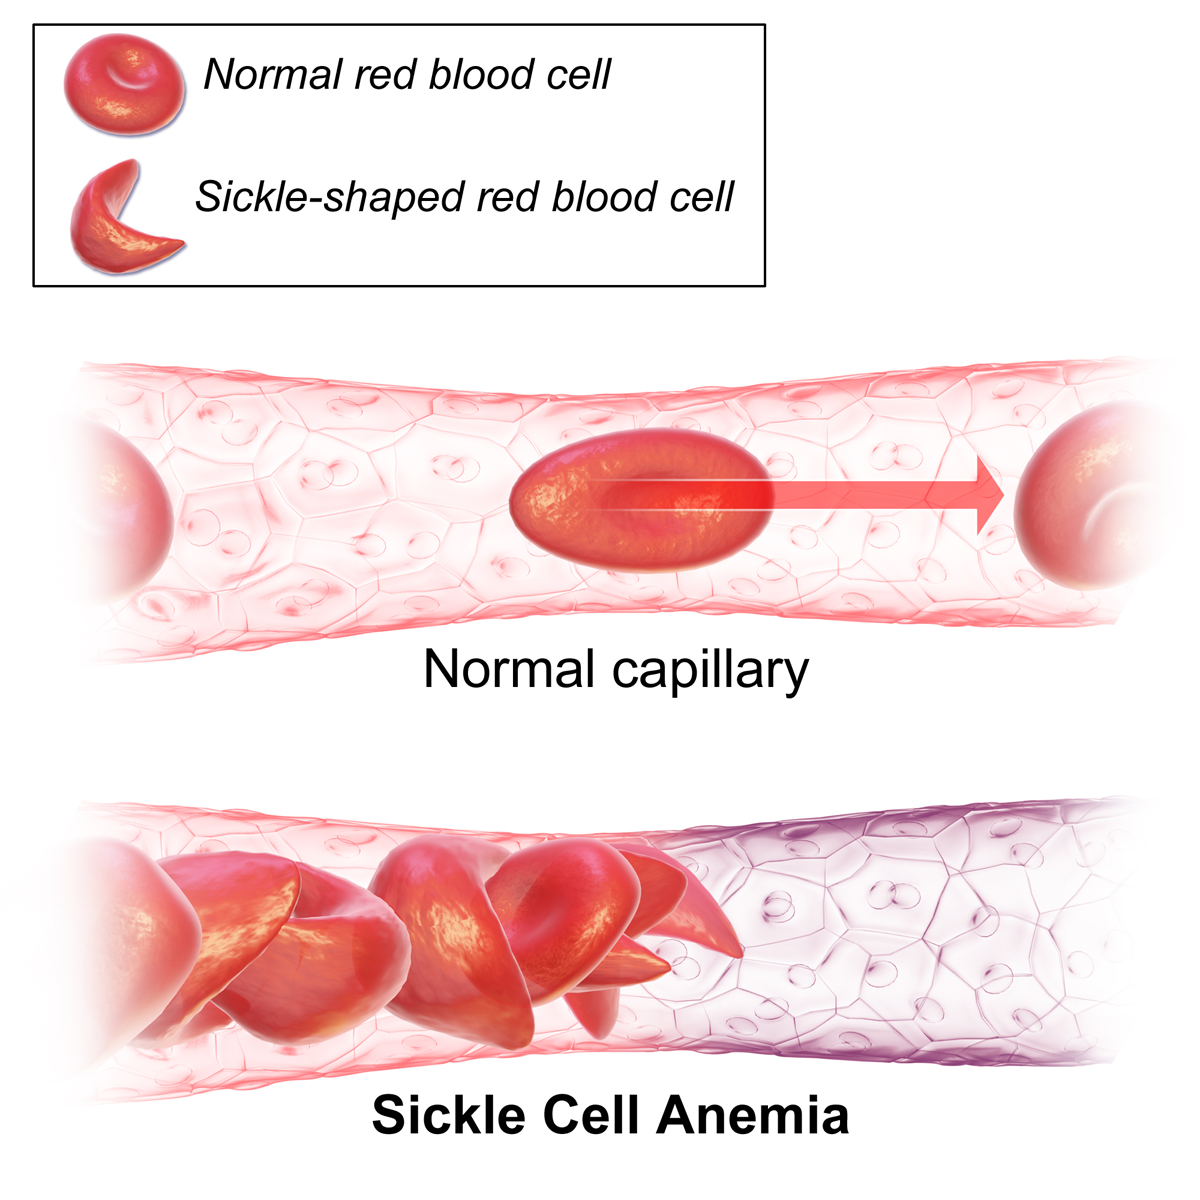
\includegraphics[width=0.45\linewidth]{./figs/Sickle_Cell_Anemia_wiki3} 

}

\caption{Misvormde rode bloedcellen bij patiënten met sikkelcelanemie (Bron: Wikipedia)}\label{fig:sickleCell2}
\end{figure}

Evolutie is dus een natuurlijk proces dat wordt aangedreven door twee tegengestelde krachten: variatie en selectie.

Variatie ontstaat onder andere door spontane kopieerfouten in genetische code of mutaties.

Selectie vindt plaats op basis van ecofactoren: is een mutatie gunstig of schadelijk voor een bepaald organisme in zijn specifieke omgeving? De kans op fixatie van de mutatie hangt dus af van het reproductiesucces.

Het proces van genetische variatie en selectie kan uiteindelijk na vele generaties leiden tot de evolutie van nieuwe soorten.

\hypertarget{genetische-drift}{%
\subsection{Genetische Drift}\label{genetische-drift}}

Een ander belangrijk proces voor het ontstaan van soorten is genetische drift. Dit zijn willekeurige fluctuaties van allelen, dit zijn specifieke sequentievarianten van een gen. Genetische drift is vooral sterk in kleine populaties. In tegenstelling tot selectie is het niet adaptief.

Nieuwe soorten zullen dus sneller ontstaan wanneer een klein deel van de populatie geïsoleerd raakt in een nieuwe omgeving.

\hypertarget{horizontale-genoverdracht}{%
\subsection{Horizontale Genoverdracht}\label{horizontale-genoverdracht}}

Horizontale genoverdracht of de niet-seksuele overdracht van genetische informatie tussen twee verschillende organismen is ook belangrijk voor het evolutionaire proces.

Dit komt veel voor bij Prokaryota, dat wil zeggen eubacteriën en archaea-bacteriën, denk maar aan de superbacteriën in ziekenhuizen die resistentie hebben verworven tegen meerdere vormen van antibiotica. Het komt ook voor tussen Eukaryota. Vooral bij protisten, eencellige organismen met een kern. Evenals tussen Prokaryota enerzijds en Eukaryota anderzijds.

\hypertarget{endosymbiose}{%
\subsection{Endosymbiose}\label{endosymbiose}}

Eldredge en Gould hebben aangetoond dat het fossielenbestand aangeeft dat de evolutie in uitbarstingen plaatsvindt: meestal gaat het langzaam totdat er in korte tijd plotseling snelle veranderingen optreden \citep{margulis1999}. Volgens Margulis kan dit worden verklaard door endosymbiose, waarbij de ene soort binnen een andere soort gaat leven. Dat is een bron van evolutionaire vernieuwing die aanleiding kan geven tot een explosie van nieuwe levensvormen.

Er bestaan twee archetypen van cellen:

\begin{itemize}
\tightlist
\item
  Prokaryota, alle bacteria en archaebacteria, die zijn ééncellig en bestaan uit een eenvoudige cel met een grootte van 0,1 tot 5,0 \(\mu m\) met DNA dat vrij in het celcytosol (de vloeistof in de cel) ligt, zie Figuur \ref{fig:prokaryotaCell} en
\end{itemize}

\begin{figure}

{\centering 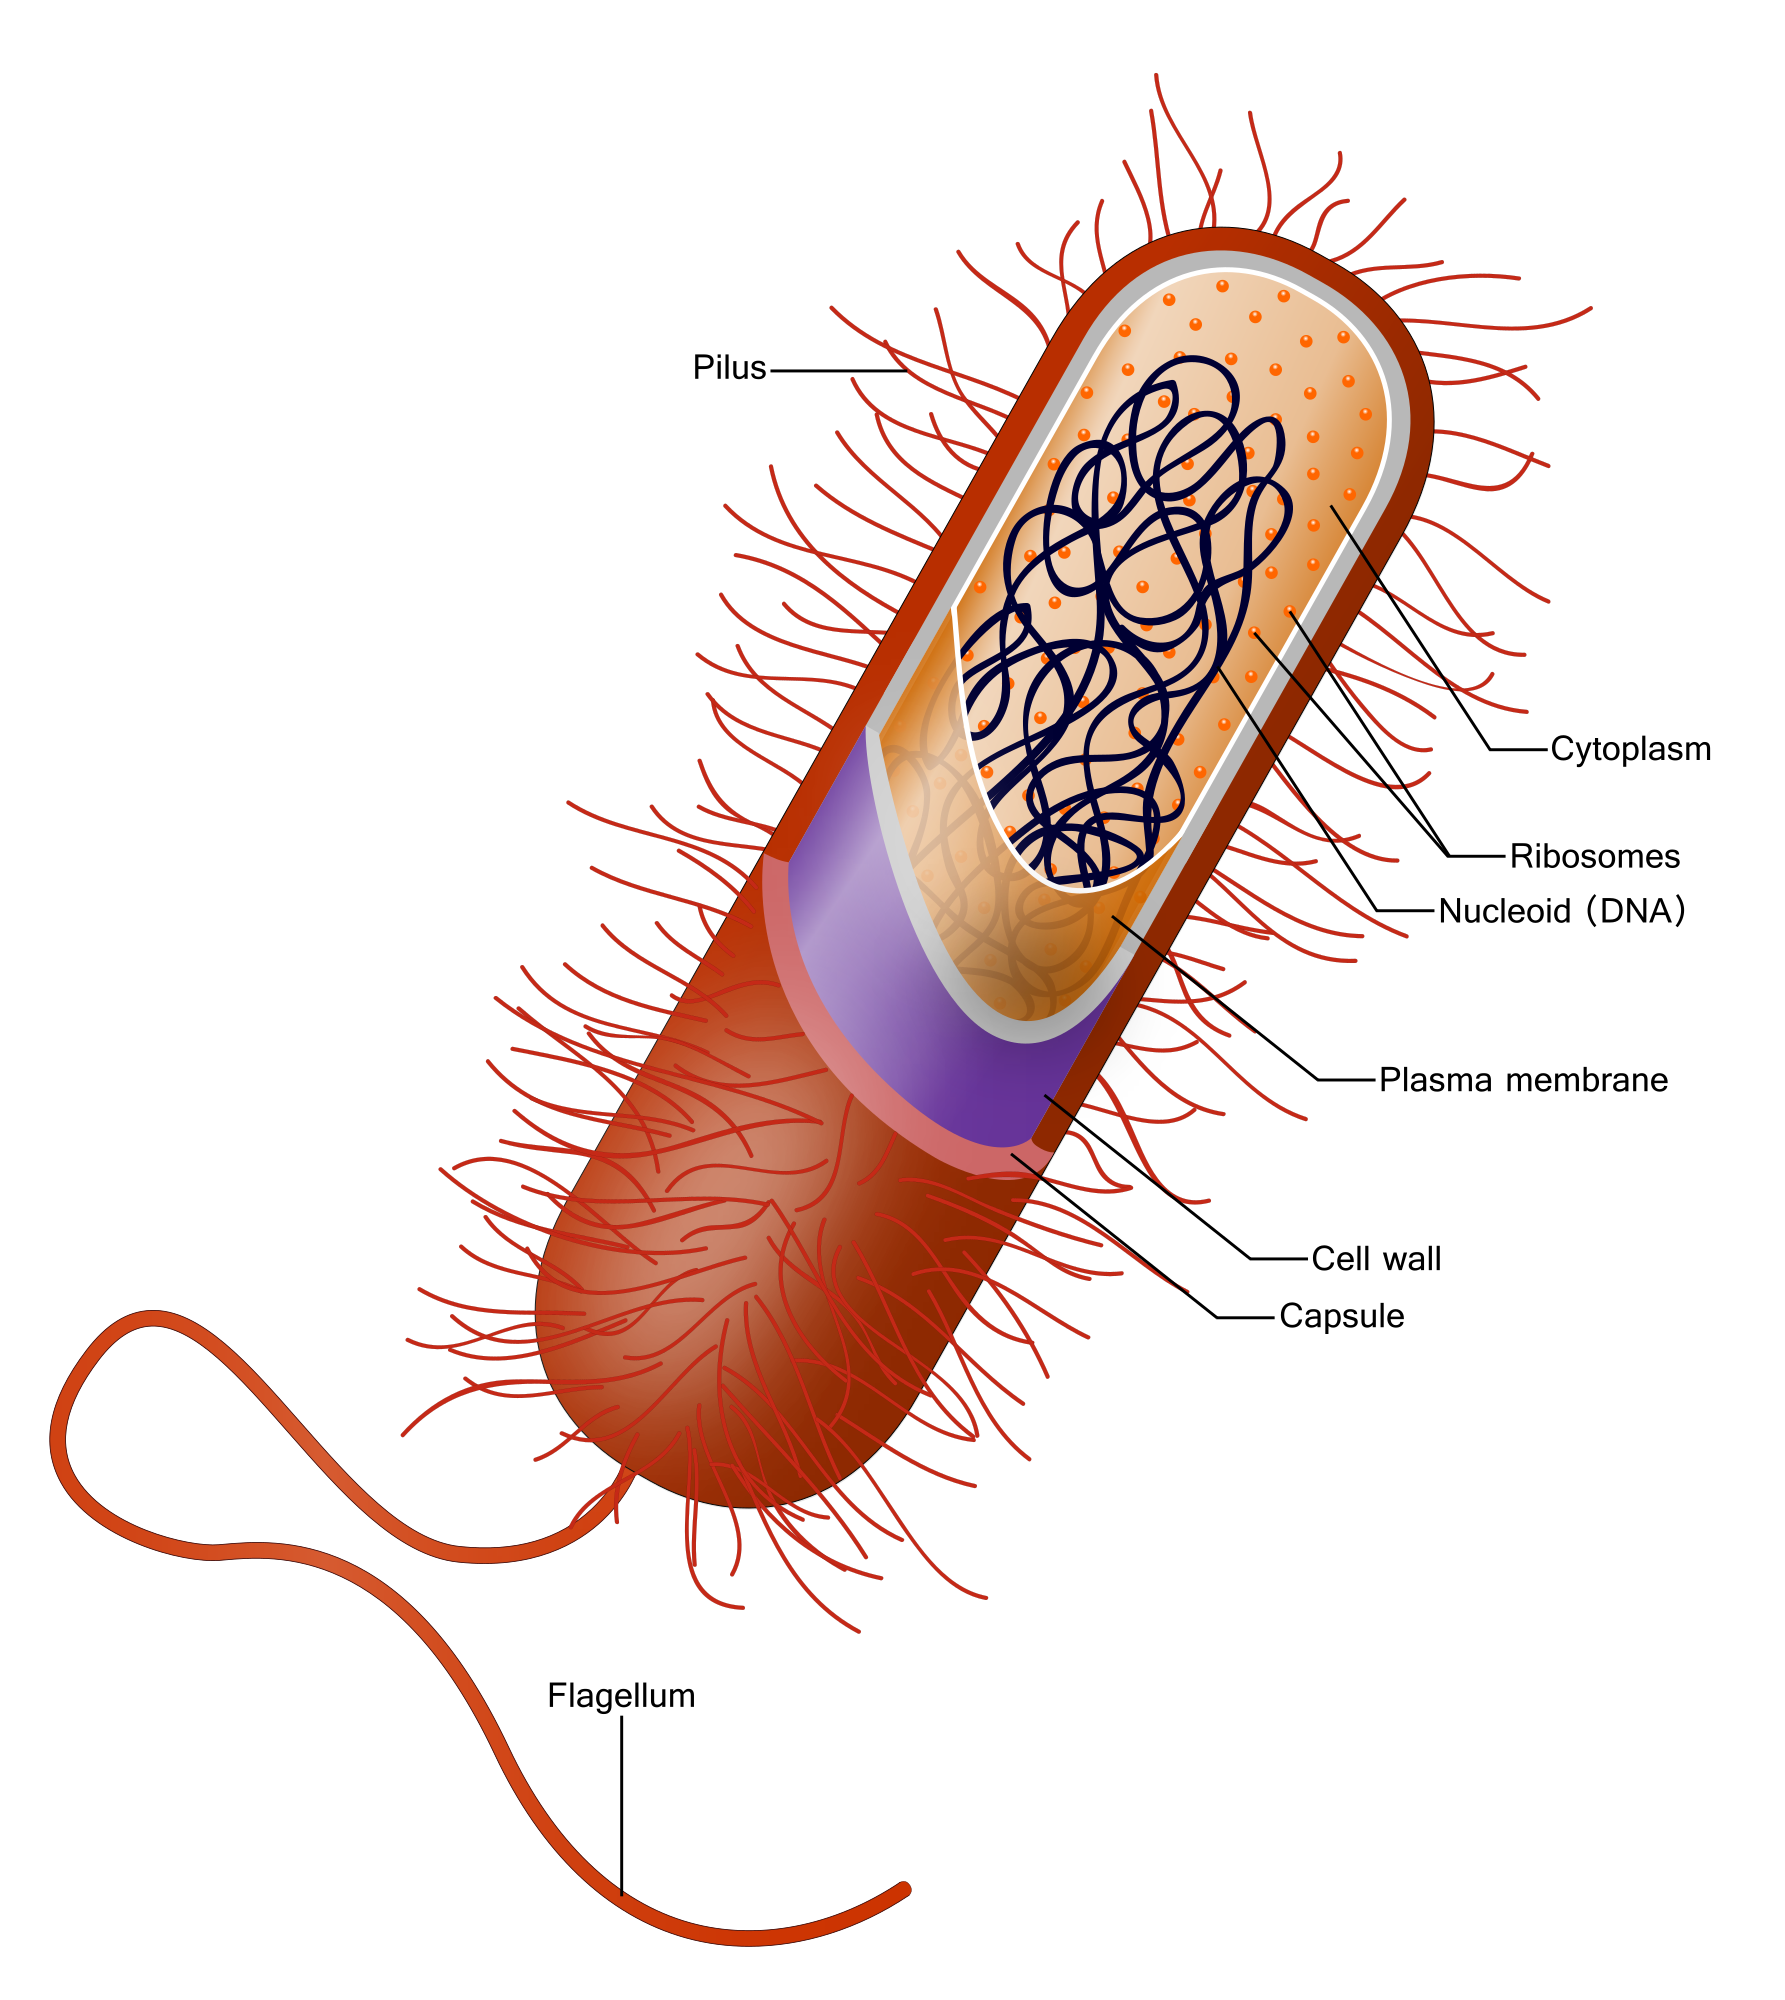
\includegraphics[width=0.5\linewidth]{./figs/prokaryoteCell} 

}

\caption{ Diagram van een typische prokaryote cel. De cel is eenvoudig, het DNA ligt vrij in de cel (Bron: Ali Zifan, Wikipedia)}\label{fig:prokaryotaCell}
\end{figure}

\begin{itemize}
\tightlist
\item
  Eukaryota, protisten, schimmels, planten en dieren, die zijn ééncellig of meercellig en hebben grotere en meer complexe cellen, 10-100 \(\mu m\) groot. Ze hebben interne membraangebonden structuren, organellen genaamd, en een cytoskelet, die een belangrijke rol spelen bij het de organisatie en vorm van de cel. Eukaryotisch DNA wordt opgeslagen in chromosomen. Een chromosoom is een lang DNA-molecule dat in compacte vorm is opgeslagen. Een chromosoom bevat een deel of al het genetische materiaal van een organisme. Menselijke cellen hebben 46 chromosomen, dat wil zeggen 23 chromosoomparen. Elk paar bestaat uit één exemplaar van onze biologische moeder en één exemplaar van onze biologische vader. De chromosomen bevinden zich in de celkern, het organel dat de integriteit van de chromosomen en dus van onze genen in stand houdt, en speelt een belangrijke rol bij de regulatie van genexpressie en van de activiteit van de cel. Zie Figuren \ref{fig:animalCell} and \ref{fig:plantCell}.
\end{itemize}

\begin{figure}

{\centering 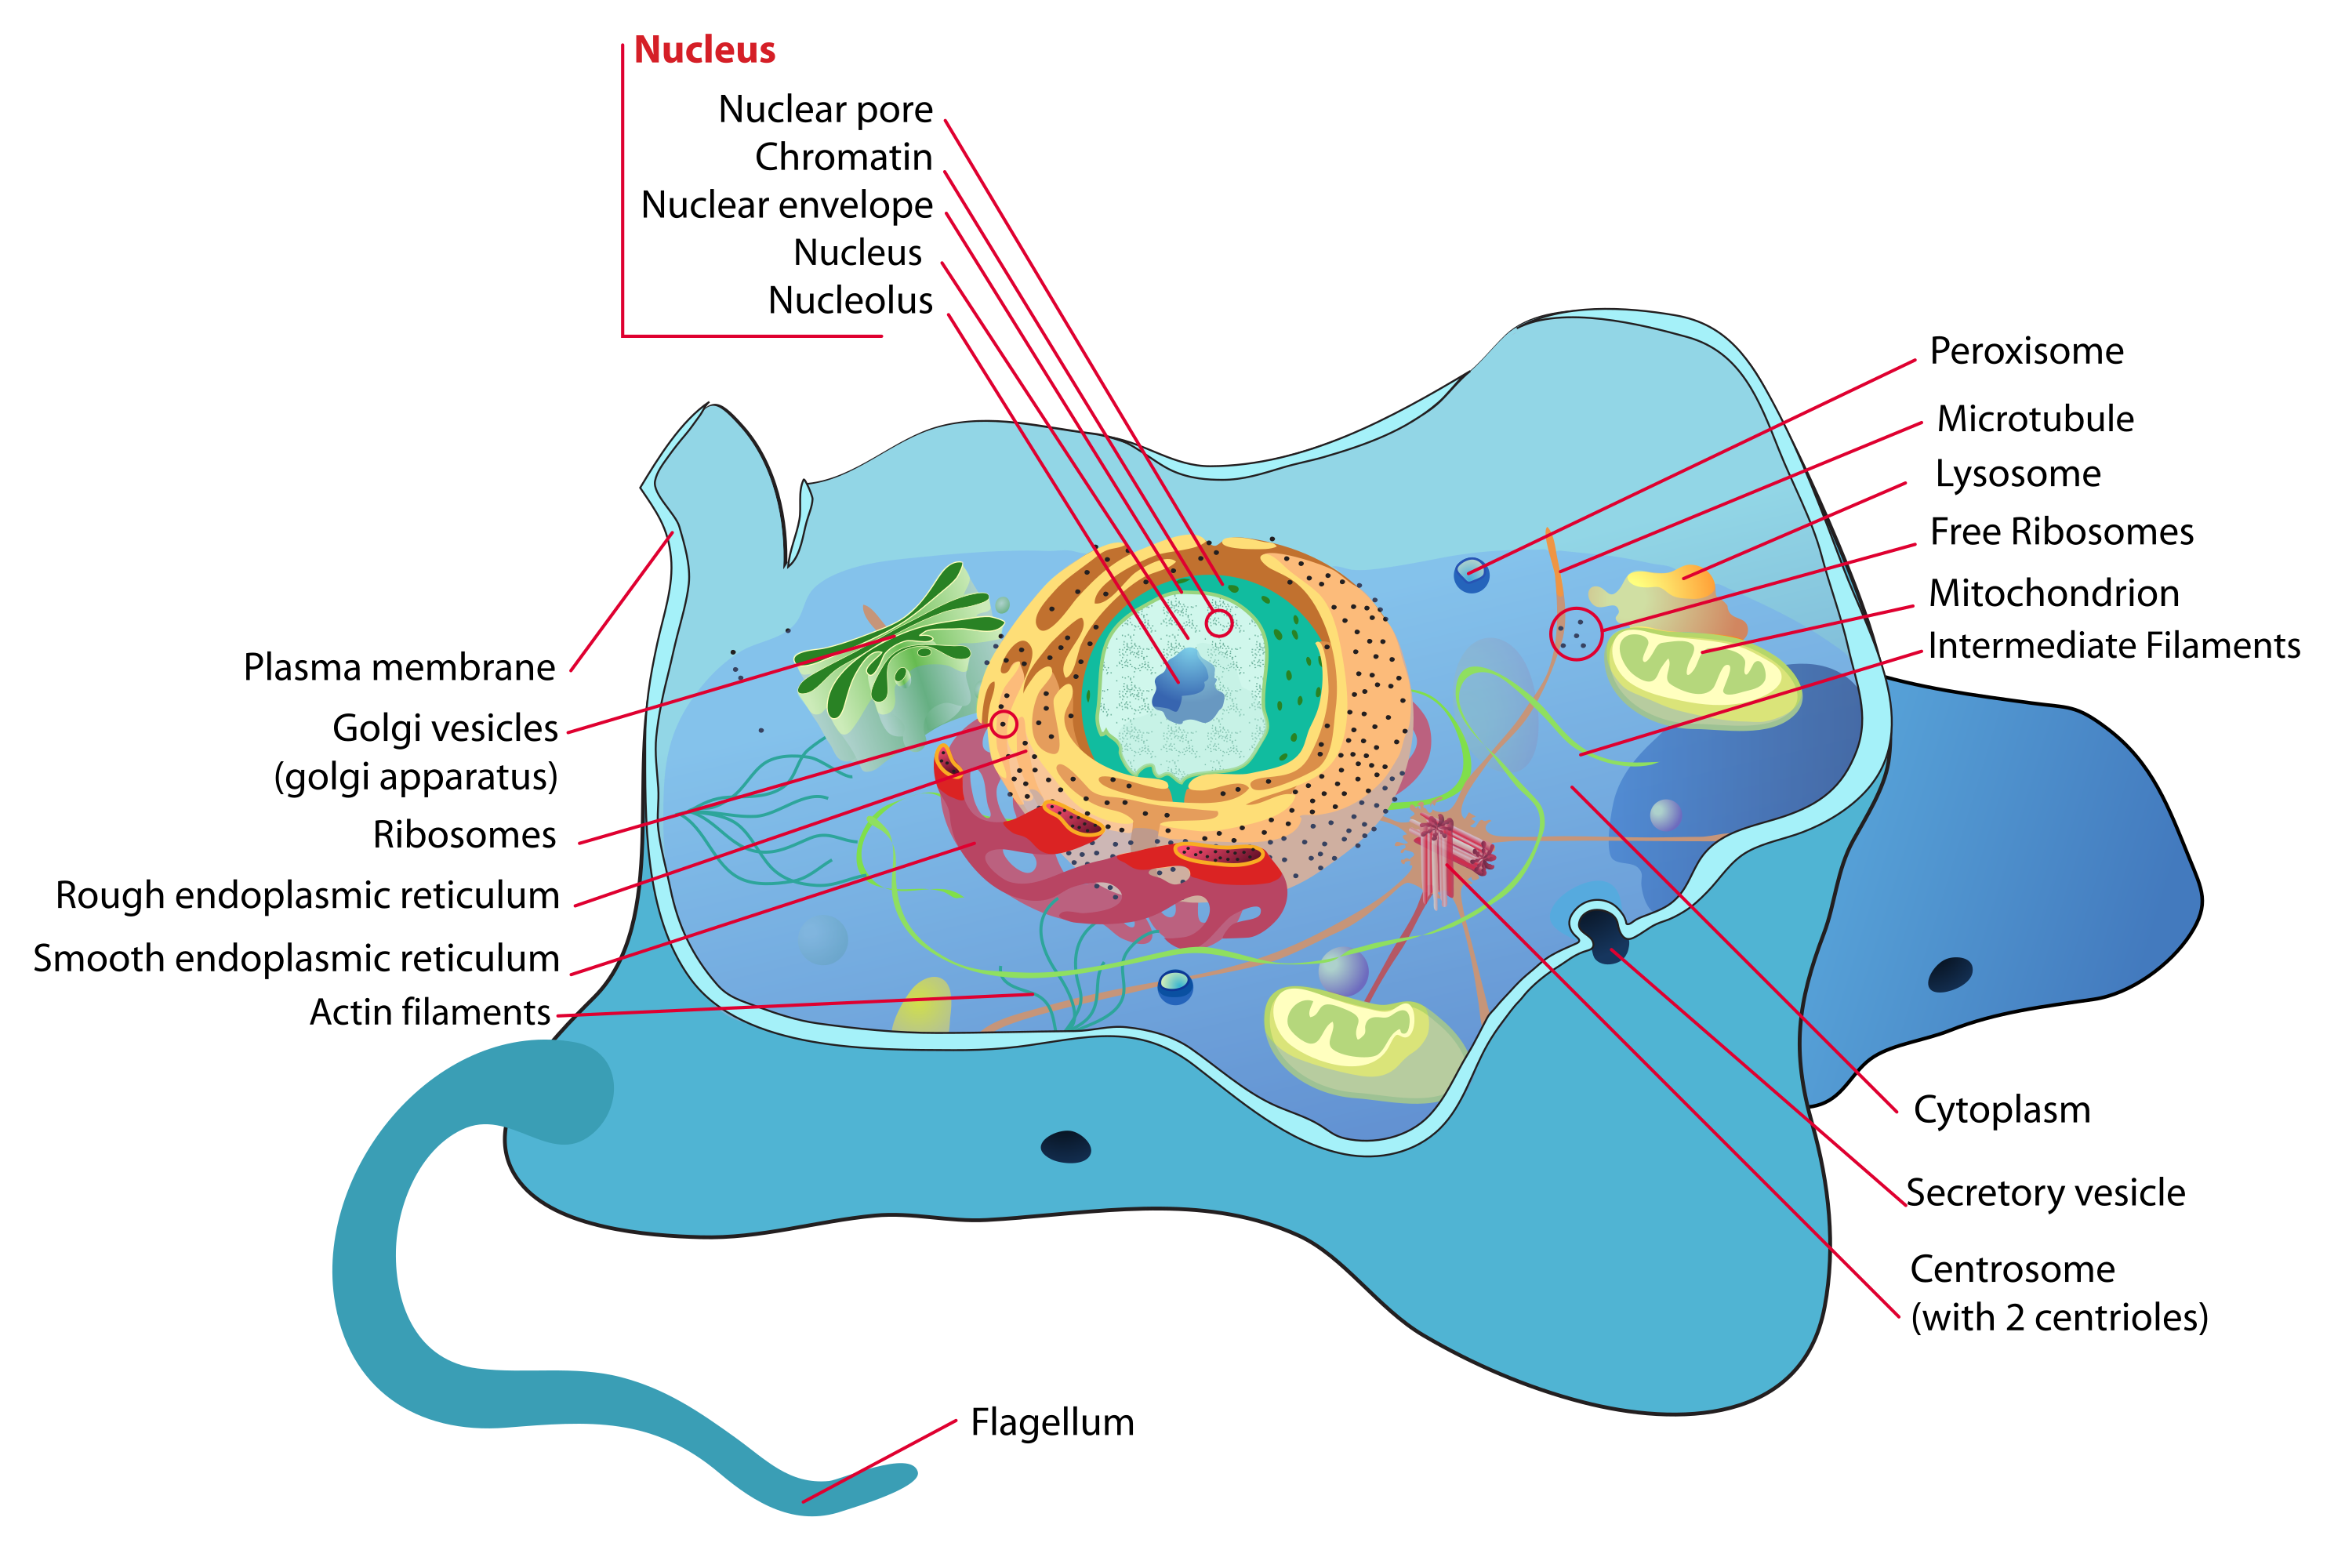
\includegraphics[width=0.5\linewidth]{./figs/animalCell} 

}

\caption{Diagram van een typische dierlijke cel. Dierlijke cellen zijn eukaryotische cellen. Ze zijn doorgaans veel groter dan die van prokaryoten. Ze hebben interne membraangebonden structuren, organellen genaamd, en een cytoskelet, die een belangrijke rol spelen bij de organisatie en vorm van de cel. Eukaryoot DNA is verdeeld in chromosomen, die zich in de celkern bevinden, het organel dat de integriteit van genen handhaaft, en een belangrijke rol speelt bij de regulatie van genexpressie en van de activiteit van de cel. (Bron:  Mariana Ruiz Villarreal, Wikipedia)}\label{fig:animalCell}
\end{figure}

\begin{figure}

{\centering 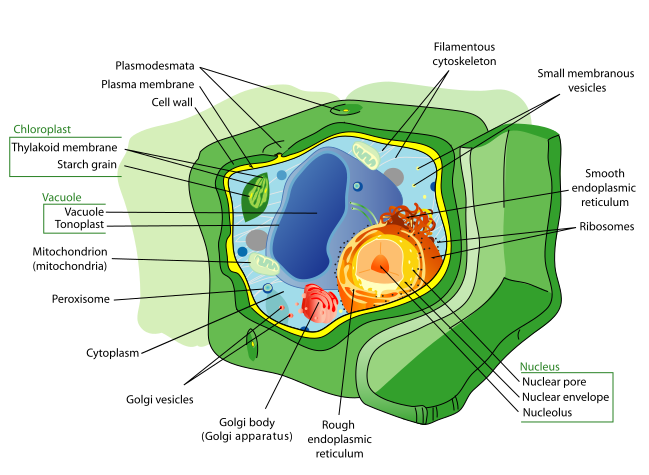
\includegraphics[width=0.5\linewidth]{./figs/plantCell} 

}

\caption{Diagram van een typische plantencel. Plantcellen zijn eukaryotische cellen. Ze zijn doorgaans veel groter dan die van prokaryoten. Ze hebben interne membraangebonden structuren, organellen genaamd, en een cytoskelet, die een belangrijke rol spelen bij de organisatie en vorm van de cel. Eukaryoot DNA is verdeeld in chromosomen, die zich in de celkern bevinden, het organel dat de integriteit van genen handhaaft, en een belangrijke rol speelt bij de regulatie van genexpressie en de activiteit van de cel. Plantencellen hebben ook een celwand en bladgroenkorrels die aan fotosynthese kunnen doen. (Bron:  Mariana Ruiz Villarreal, Wikipedia)}\label{fig:plantCell}
\end{figure}

Van 3,5 BYA - 540 MYA vindt men voornamelijk prokaryotische en enkele eenvoudige eukaryote organismen in fossielen en was het leven voornamelijk eencellig.

De sequentiële endosymbiosetheorie (SET) van Margulis stelt dat eukaryote cellen werden gegenereerd door endosymbiose, dat is een symbiotische relatie waarbij het ene organisme in het andere begon te leven, wat gunstig is voor beide organismen. Het proces van sequentiële endosymbiose dat leidde tot eukaryote cellen wordt weergegeven in Figuur \ref{fig:endosymbiosis}.

\begin{figure}

{\centering \includegraphics[width=0.8\linewidth]{./figs/endosymbiosis} 

}

\caption{Ontstaan van eukaryote cellen (Bron: wikipedia)}\label{fig:endosymbiosis}
\end{figure}

Er wordt aangenomen dat eerst een anaerobe\footnote{Anaeroob: leven in afwezigheid van zuurstof} prokaryote cel was gegroeid en membraansystemen in de cel had ontwikkeld, wat aanleiding gaf tot de vorming van de kern\footnote{Merk op dat volgens Margulis de grote anaërobe cel met een kern, de eerste eukaryoot, al het resultaat was van een eerdere endosymbiotische gebeurtenis. Er bestaat echter nog geen wetenschappelijke consensus over deze hypothese.}.
Op een gegeven ogenblik moet deze grote prokaryotische cel met interne membraansystemen een aërobe\footnote{Aëroob: zuurstofgebruik en ademhaling met zuurstof, dat levert meer energie op} proteobacterie hebben opgeslokt, die erin slaagde om niet te worden gemetaboliseerd. De twee cellen begonnen met een endosymbiotische relatie.

De opgeslokte proteobacterium voorzag de gastheercel van extra energie door koolhydraten en lipiden te metaboliseren met behulp van zuurstof en de gastheercel voedde de proteobacterium met deze biomoleculen. Dit gaf het endosymbiotische paar de mogelijkheid om verder in omvang te groeien en te gedijen in de zuurstofrijke omgeving van planeet Aarde die ontstond tijdens het Cambrium-tijdperk dat 540 miljoen jaar geleden begon. Aangenomen wordt dat de toename van zuurstof één van de belangrijkste triggers is die aanleiding gaf tot de `biologische oerknal' die leidde tot een explosie van nieuwe soorten en de opkomst van alle grote groepen\footnote{Grote groepen van een koninkrijk worden meer formeel \emph{phyla} genoemd} in het dierenrijk \citep{he2019}.

Tijdens hun endosymbiotische evolutie droeg de proteobacterium geleidelijk veel genen over aan de celkern, en kwam onder regulatie van de kern te staan. Uiteindelijk evolueerde de proteobacterium naar mitochondriën, de organellen die de energiefabrieken van een cel zijn. We erven dus meer van moeder dan van vader: we erven zowel onze celstructuur als ons energiesysteem, dat wil zeggen onze mitochondriën en hun resterende DNA, van moederskant via haar eicel.

Voor plantencellen moet een tweede endosymbiotische gebeurtenis hebben plaatsgevonden met eukaryotische cellen en cyanobacteriën. De opgeslokte cyanobacteriën zijn op een vergelijkbare manier geëvolueerd tot chloroplasten. Deze geven planten het vermogen tot fotosynthese en hebben ervoor gezorgd dat ze de meest succesvolle levensvorm ter wereld zijn geworden. Fossiel bewijs van landplanten dateert uit 485 MYA - 420 MYA, maar fylogenetische analyse suggereert een eerdere oorsprong in het Cambrium \citep{StrotherFoster2021}.

Andere belangrijke verschillen tussen Prokaryota en Eukaryota zijn hun reproductie. Bij Prokaryota gebeurt dat alleen door celdeling. Een mutatie in het DNA wordt dus in alle dochtercellen vastgelegd. Terwijl bijna alle Eukaryota een fase van seksuele voortplanting hebben. Het zijn diploïde organismen, dat wil zeggen dat ze van elk gen twee kopieën hebben, één van vaders- en één van moederskant. Hierdoor kunnen opeenvolgende mutaties in één kopie worden gemaakt, omdat er een andere functionele kopie van het gen beschikbaar is. Bovendien vindt tijdens seksuele voortplanting recombinatie van chromosomen plaats, dat wil zeggen een herschikking van vader- en moedergenen, wat tot veel meer variatie leidt.

De Eukaryota evolueerden verder in protisten, dit zijn eencellige organismen, schimmels, planten en dieren. De SET-theorie van Margulis ondersteunt ook een meer intuïtieve organisatie van de levensboom in een tweedelige (eukaryote versus prokaryote) taxonomie van vijf koninkrijken die de evolutionaire geschiedenis weerspiegelt, zie Figuur \ref{fig:fiveKingdoms}: Prokaryotische bacteriën en archae-bacteriën, die samen het koningkrijk van de Prokaryoten (of Monera) vormen, evolueerden in eukaryote Protista en die evolueerden verder naar Planten, Schimmels en Dieren.

\begin{figure}

{\centering 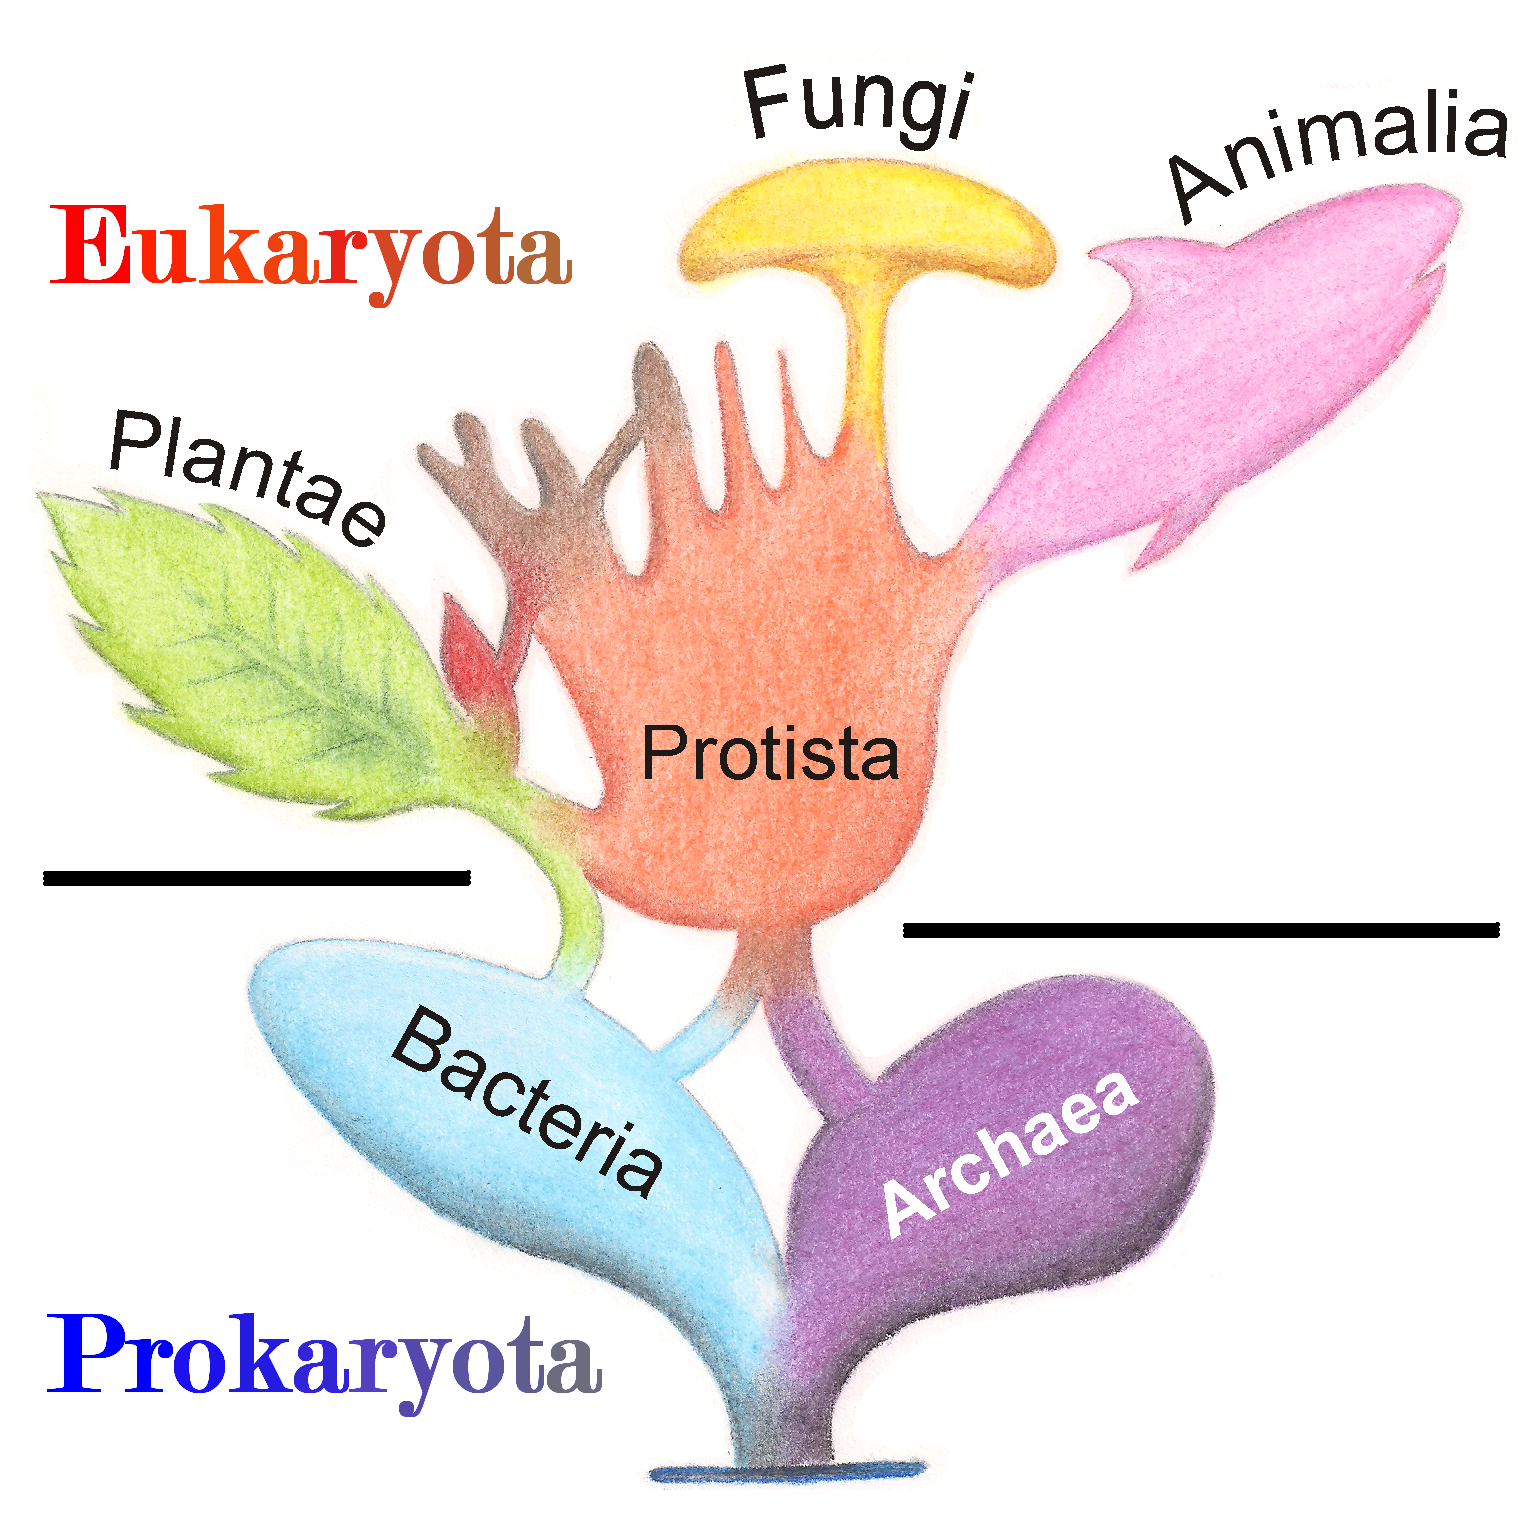
\includegraphics[width=0.8\linewidth]{./figs/fiveKingdoms} 

}

\caption{Tweedelige (eukaryote versus prokaryotische) taxonomie van vijf koninkrijken die de evolutionaire geschiedenis weerspiegelt: Prokaryotische bacteriën en archae-bacteriën, die samen het koningkrijk van de Prokaryoten (of Monera) vormen, evolueerden naar eukaryotische Protista die zich verder ontwikkelde tot planten, schimmels en dieren (Bron: wikipedia)}\label{fig:fiveKingdoms}
\end{figure}

\hypertarget{symbiose-en-symbiogenese}{%
\subsection{Symbiose en Symbiogenese}\label{symbiose-en-symbiogenese}}

Deze sectie is grotendeels gebaseerd op Margulis' boek ``The symbiotic Planet'' \citep{margulis1999}.

Volgens Margulis is symbiose cruciaal om evolutionaire vernieuwing en de oorsprong van soorten te begrijpen.

Symbiogenese is een evolutionaire term die verwijst naar de oorsprong van nieuwe weefsels, organen, organismen en zelfs soorten door het tot stand brengen van langdurige en permanente symbiose. Zoals Margulis argumenteerde: ``alle organismen die groot genoeg zijn om te zien, zijn samengesteld uit ooit onafhankelijke micro-organismen die samenwerken in grotere gehelen.'' Het feit dat schimmel-, planten- en dierencellen zijn ontstaan door endosymbiose wordt nu algemeen aanvaard. Symbiotische fusies gingen echter door in de evolutionaire geschiedenis en waren uiterst belangrijk voor het leven om de hele wereld te koloniseren.

Het leven ontwikkelde zich inderdaad in de zee en symbiose was de drijvende kracht achter de kolonisatie van het onherbergzame droge land. De symbiose tussen schimmels en cyanobacteriën of groene algen waaruit korstmossen ontstaan, is bijvoorbeeld essentieel geweest voor de kolonisatie van het droge rotsachtige landoppervlak en om die in vruchtbare grond te veranderen. Het belang van korstmossen blijkt duidelijk uit hun biomassa, die naar schatting zelfs groter is dan de biomassa van al het leven in de oceaan.

Als er eenmaal grond beschikbaar is, kunnen planten het leven overnemen. Ook het plantenleven is weer in grote mate afhankelijk van hun symbiose met schimmels. Plantenwortels en schimmels vormen inderdaad mycorrhiza's die gezwollen symbiogenetische structuren zijn. De schimmel voorziet de plant van minerale voedingsstoffen en de plant op zijn beurt voorziet zijn schimmelpartner van sap of fotosynthetisch voedsel. Hun huwelijk maakte planten tot het meest succesvolle koninkrijk in termen van de hoeveelheid koolstof die ze fixeren.

Soortgelijke voorbeelden gelden ook voor dieren. Herkauwers, zoals bijvoorbeeld runderen, schapen, antilopen, herten, giraffen, zouden nooit geëvolueerd zijn zonder hun symbiose met cellulose-afbrekende protisten die hen in staat stellen gras te verteren. Hetzelfde geldt voor ons mensen: de symbiose met de micro-organismen in onze darmen, ons darmmicrobioom, is cruciaal voor ons om ons voedsel te verteren.

\hypertarget{teleonomie}{%
\subsection{Teleonomie}\label{teleonomie}}

Teleonomie is de kwaliteit van schijnbare doelgerichtheid van structuren en functies in levende organismen, tot stand gebracht door evolutionaire aanpassing. Door de hele evolutionaire geschiedenis heen is er dus nooit een ander doel geweest om een bepaalde eigenschap te ontwikkelen dan het primitieve doel om de soort in stand te houden en te reproduceren.

Wanneer complexe organen en organismen ontstaan lijkt het misschien alsof er een richting of doel is, maar dat is niet het geval!

Zoals \citet{rosenberg2008} mooi verwoorden in hun boek ``Phylosophy of Biology''\footnote{Sectie Misunderstandings about natural selection p20}: ``De theorie van Darwin bezorgt voor sommigen verwarring met betrekking tot complexiteit, willekeur en richting. Ze vragen zich af hoe complexe functionele ontwerpen kunnen ontstaan door een willekeurig proces zoals natuurlijke selectie. De evolutie van een complexe structuur zoals een vleugel (zoals bij een vogel) vanaf een vin (zoals bij een primitieve vis) lijkt misschien onmogelijk, gezien de willekeur van het proces van natuurlijke selectie en de enorme aantal aanpassingen die nodig zijn.''

``Het eerste deel van het antwoord is dat natuurlijke selectie niet willekeurig is. Het is een proces dat willekeur als \emph{input} vereist. De variaties die ontstaan zijn niet gericht op het oplossen van problemen die door de omgeving worden veroorzaakt. Maar de \emph{uitkomst} van natuurlijke selectie is beslist niet willekeurig: het verschil in overleving en reproductie van de varianten die beter aangepast zijn.''

``Het tweede deel van het antwoord is dat natuurlijke selectie cumulatief kan werken, en dat maakt complexe aanpassingen mogelijk. Selectie transformeerde eerst een vin in een ledemaat om mee te lopen die sterk genoeg was om een groot dier op het land te ondersteunen, en het transformeerde later van een lopend ledemaat in een vleugel. Complexiteit is mogelijk omdat latere aanpassingen voortbouwen op eerdere aanpassingen. Met andere woorden, complexe aanpassingen worden niet met grote sprongen tot stand gebracht, maar in kleinere stappen, die stuk voor stuk adaptief zijn, en de functie die kan van de ene stap naar de volgende veranderen. Een vleugel is geen betere vin of zelfs geen beter been. Het is iets heel anders, het heeft een andere functie. Als we alleen naar de eindresultaat kijken, lijkt de overbrugde kloof onmogelijk groot, en dat komt deels omdat natuurlijke selectie tot op zekere hoogte haar sporen bedekt. Als we naar een vin of vleugel kijken, is het tussenliggende stadium van de lopende ledematen niet onmiddellijk duidelijk. Hoewel natuurlijke selectie zijn sporen uitwist, is er veel werk in de biologie besteed aan het blootleggen ervan. Één van Darwins eerste argumenten voor natuurlijke selectie was gebaseerd op de grote gelijkenis in delen, hun aantal en de homologie van de botten in vinnen, poten en vleugels. Tweehonderd jaar later kunnen moleculair biologen de genealogie van de vleugel van de vogel terugvoeren via de poot van het reptiel tot aan de vin van de vis, in de overeenkomsten en verschillen van de gensequenties die de ontwikkeling van elk daarvan bepalen. De verschillen en overeenkomsten in de DNA-sequentie tussen de genen die betrokken zijn bij de ontwikkeling van ledematen bij vogels, reptielen en vissen stellen ons in staat om hun gemeenschappelijke voorouders te dateren en iets te zeggen waaraan de homologieën (overeenkomst) en de verschillen tussen de botten van hun verschillende ledematen te wijten zijn.''

\begin{figure}

{\centering 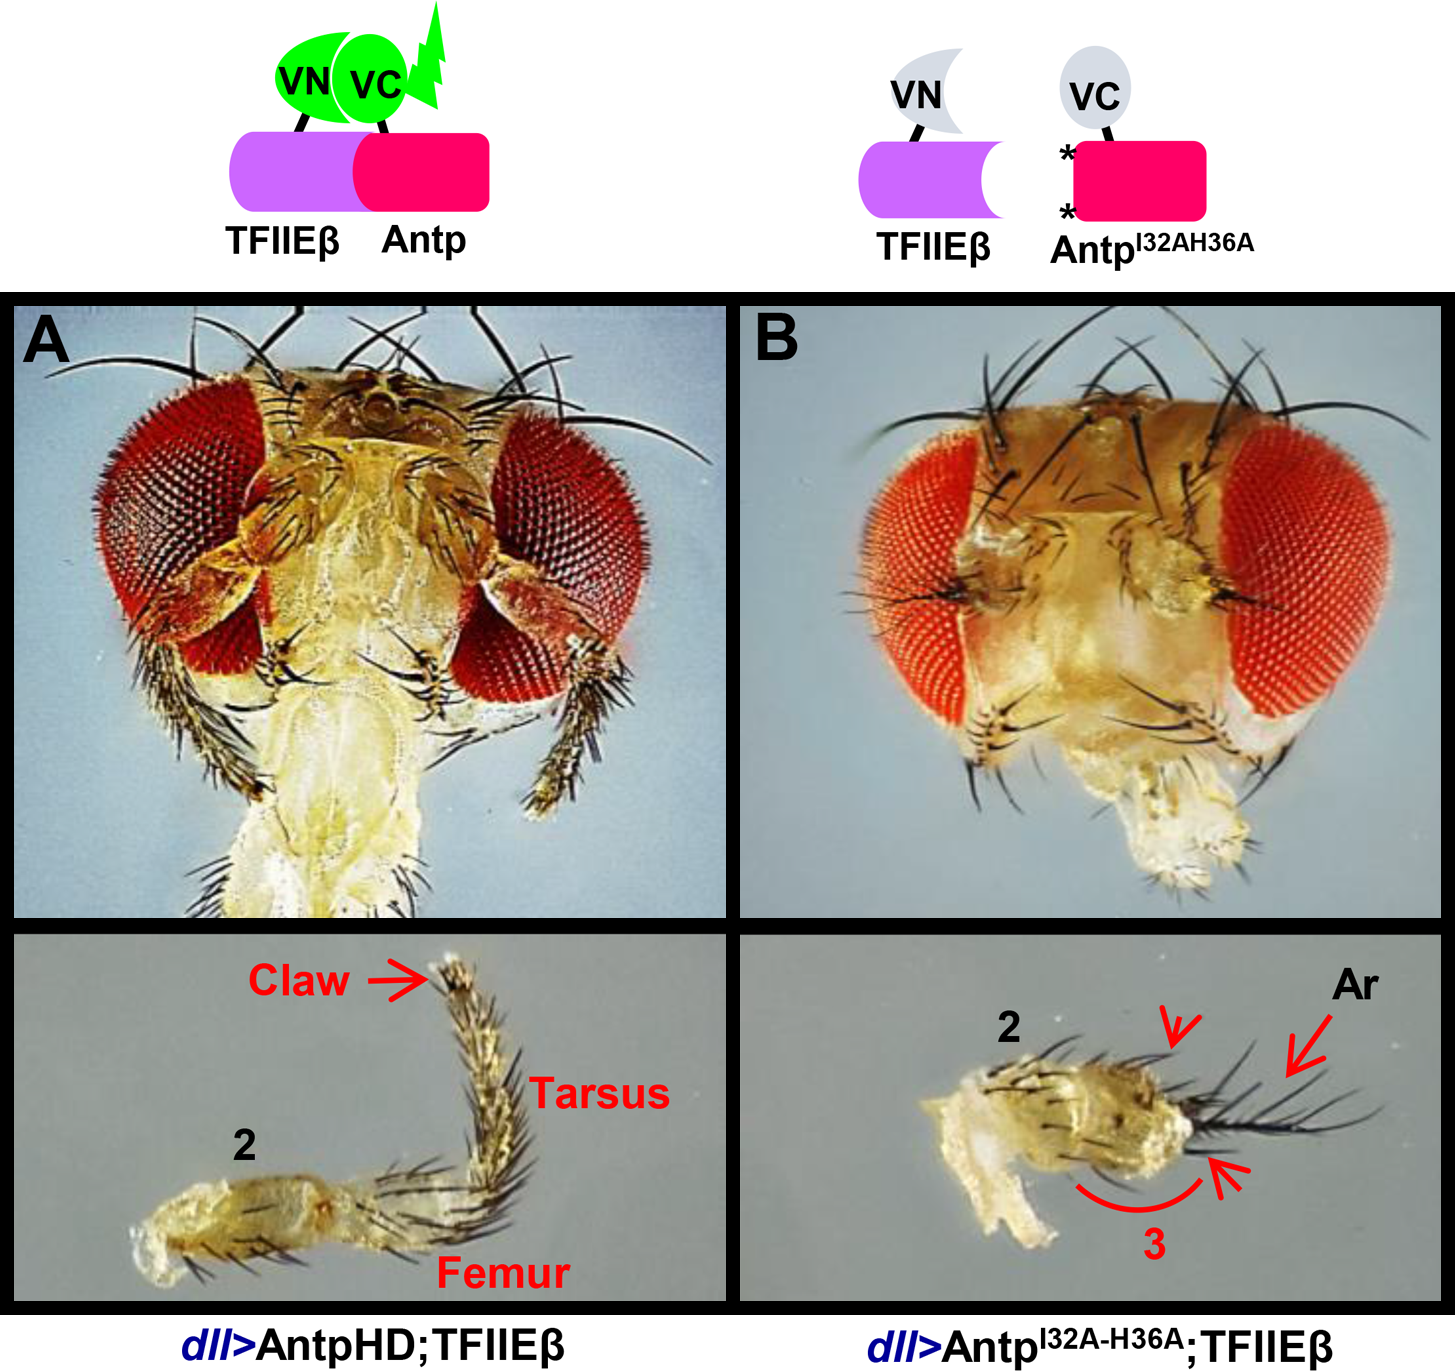
\includegraphics[width=0.45\linewidth]{./figs/pone.0205905.g006_flyAntennaLegMutation2} 

}

\caption{Een kleine mutatie kan soms grote fenotypische veranderingen veroorzaken. De mutatie van het Antp-gen leidt tot vervorming van de antenne tot een poot bij vliegen [@flyMut]. A: Kop van een vlieg met een vervorming van zijn antennes naar poten.l B: Kop van een vlieg met een normale antennevorming}\label{fig:flyEye}
\end{figure}

Bovendien brengen grote fenotypische veranderingen vaak zeer kleine genomische veranderingen met zich mee. \citet{rosenberg2008} vervolgen dat ``bij de fruitvlieg Drosophila bekend is dat een kleine mutatie in het juiste gen voldoende is om zijn antennes in een paar poten te veranderen. De moleculaire biologie is steeds beter in staat de sporen bloot te leggen die de evolutie verborgen heeft gehouden, zodat aanpassingen verwacht kunnen worden in plaats van wonderbaarlijk te zijn. Hoe zit het met de richting? Het idee van cumulatieve verandering lijkt misschien een soort gerichtheid van het aanpassingsproces te suggereren, een drang naar grotere complexiteit. In feite is het een open vraag of er in de evolutie sprake is van een voorkeur naar complexiteit toe. Wat echter duidelijk is, is dat niets in het huidige begrip van natuurlijke selectie een drang naar grotere complexiteit voorspelt. Er komen toenames voor in complexiteit, maar door onze fascinatie ervoor hebben we de neiging de frequente afnames in complexiteit te negeren. Gevleugelde dieren worden vleugelloos, zoals in de evolutie van pinguïns. Dieren met lopende ledematen verliezen deze wanneer ze terugkeren naar het water, zoals in de evolutie van walvissen (die een gemeenschappelijke voorouder hebben met nijlpaarden). Complexiteit is omkeerbaar, en selectie zal naar verwachting de voorkeur geven aan een afname wanneer zich mogelijkheden voor adaptieve eenvoud voordoen\ldots{} en dat kan vaak voorvallen!''

Daarom is de oorsprong van een soort het resultaat van evolutie, maar niet het doel van evolutie. Evolutie is dus aanpassing met als enig doel behoud en voortplanting.

Bovendien is het uit de verdeling van de complexiteit van soorten in Figuur \ref{fig:distributionComplexity}, duidelijk dat de meest voorkomende levensvormen altijd bacteriën zijn geweest. De verdeling van complexiteit heeft momenteel echter een staart naar rechts. Dit komt voort uit het feit dat er een ondergrens is voor de complexiteit van levende organismen. Daardoor kon de evolutie geen organismen voortbrengen met een complexiteit onder deze ondergrens en het lijkt daarom alleen maar alsof zij een lichte voorkeur lijkt te hebben voor een toenemende complexiteit.



\begin{figure}

{\centering 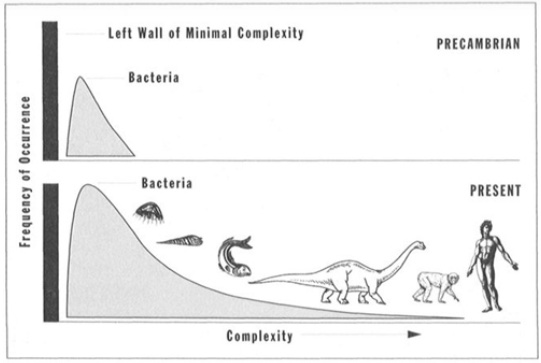
\includegraphics[width=0.45\linewidth]{./figs/selectionNoDirectionDef} 

}

\caption{Verdeling van de complexiteit van soorten \citep{gould1997}}\label{fig:distributionComplexity}
\end{figure}

\citet{Bar-On2018} publiceerden de verdeling van de koolstofmassa die wordt gefixeerd door verschillende groepen van soorten (Figuur \ref{fig:carbonFixated}), waaruit ook blijkt dat er geen voorkeur bestaat voor complexere organismen.



\begin{figure}

{\centering 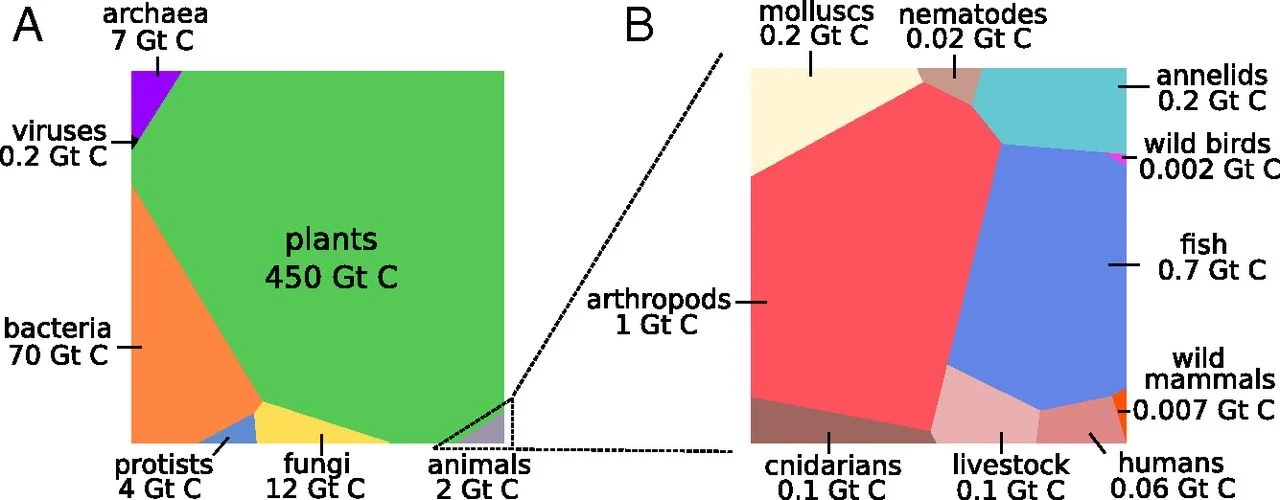
\includegraphics[width=1\linewidth]{./figs/pnas.1711842115fig01} 

}

\caption{Massa in gigaton koolstof voor verschillende groepen soorten. \citep{Bar-On2018}}\label{fig:carbonFixated}
\end{figure}

Merk op dat

\begin{itemize}
\item
  Planten de meest succesvolle groep zijn als het gaat om de hoeveelheid koolstof die ze fixeren.
\item
  Bacteriën domineren duidelijk het meer complexe dierenrijk.
\item
  Dieren vertegenwoordigen een relatief kleine fractie. Onder de zoogdieren (mammals) zijn vee en mensen oververtegenwoordigd.
\end{itemize}

Ander overtuigend bewijs dat er geen richting is voor de evolutie komt voort uit het aantal bacteriecellen in ons lichaam. \citet{Sender2016} toonden aan dat de verhouding tussen het aantal bacteriële cellen en het aantal menselijke cellen bijna 1 is. Een mens met een gewicht van 70 kg heeft 38 biljoen bacteriële cellen en 30 biljoen humane cellen. Merk op, dat een biljoen duizend miljard of 10\(^{12}\) is!

De visie van Margulis hierop wordt mooi samengevat in het volgende citaat: ``meer complexe meercellige organismen zoals schimmels, planten en dieren kunnen worden gezien als een enorme kolonie van gedifferentieerde, gefuseerde en muterende symbiotische micro-organismen'' \citep{margulis1999}.

Al deze argumenten maken dus duidelijk dat de evolutie geen richting heeft. In plaats daarvan kunnen we evolutie zien als een onvoorstelbaar creatief proces dat nieuwe levensvormen voortbrengt die goed zijn aangepast aan hun steeds veranderende omgeving. Dit inzicht in de evolutie nodigt ons dus uit om in plaats daarvan de rijkdom van diversiteit te omarmen.

\hypertarget{evolutie-mensheid-en-biodanza}{%
\section{Evolutie, Mensheid en Biodanza}\label{evolutie-mensheid-en-biodanza}}

Eerst was er

\begin{enumerate}
\def\labelenumi{\arabic{enumi}.}
\item
  Chemische evolutie: evolutie van de bouwstenen en de chemie van het leven.
\item
  Vervolgens de biologische evolutie van cellen/organismen op basis van de selectie van genetische informatie en functie.
\item
  En ten slotte heeft onze soort een culturele evolutie geïntroduceerd die de natuurlijke evolutie kan omzeilen met behulp van

  \begin{itemize}
  \tightlist
  \item
    kunstmatige selectie: fokken van planten, huisdieren, vee, genetische manipulatie, \ldots{}
  \item
    Technologie: die ons in staat stelt ons snel aan te passen aan nieuwe omgevingen.
  \end{itemize}
\end{enumerate}

Onze rechtopstaande levensstijl gaf onze handen een nieuwe vrijheid waardoor wij, homoniden, gereedschap en wapens konden maken en gebruiken. Dit stimuleerde een snelle hersenontwikkeling die uiteindelijk aanleiding gaf tot de evolutie van taal en menselijk bewustzijn, die nauw verweven is met de evolutie van technologie en sociale relaties \citep{capraLuisi2014}.

\hypertarget{bewustzijn}{%
\subsection{Bewustzijn}\label{bewustzijn}}

Met deze evolutie ontstond een tweede type bewustzijn, dat het ``uitgebreid bewustzijn'' of ``extended consciousness'' wordt genoemd (zie bijvoorbeeld \citet{capraLuisi2014}). Aan de ene kant hebben we dus een ``primair bewustzijn'' of ``primary consiousness'', dat is het cognitieve proces dat is geassocieerd met de zintuiglijke en emotionele ervaringen, die een organisme de perceptie van een ``zelf'' geeft hier en nu, en dat wijdverspreid is onder alle levende organismen. Aan de andere kant, hebben we ook een ``uitgebreid bewustzijn'' of ``extended consiousness''. Dat geeft een identiteitservaring, het vermogen tot reflectie en het maken mentale beelden, waardoor we waarden, overtuigingen, doelen en strategieën kunnen formuleren. Uit de evolutie van onze taal ontstond niet alleen een innerlijke wereld van concepten en ideeën, maar ook een sociale wereld met georganiseerde relaties en cultuur \citep{capraLuisi2014}.\\
Deze georganiseerde sociale wereld is de sleutel geweest voor ons reproductief succes. Maar het had ook diepgaande gevolgen voor ons mondiale ecosysteem, dat we op ongekende manieren hebben veranderd. Onze sociale organisatie en menselijke technologie hebben ons de gigantische sprong laten maken van mensachtigen, die doorgaans een positie in het midden van de voedselketen hadden, naar onze positie aan de top van de voedselketen \citep{Harari2015}. Andere soorten aan de top van de voedselketen evolueerden in de loop van miljoenen jaren naar die positie, waardoor ecosystemen zich langzaam aan hen konden aanpassen. Wij mensen hebben deze spectaculaire sprong echter zo snel gemaakt dat het ecosysteem en ons eigen psycho-emotionele systeem geen tijd hadden om zich aan te passen. Toppredatoren zijn majestueuze wezens vol zelfvertrouwen, aangezien ze zich in de loop van miljoenen jaren hebben ontwikkeld vrijwel zonder natuurlijke vijanden. De mensheid, daarentegen, heeft die positie zo snel ingenomen waardoor we nog steeds worden geconfronteerd met de angsten die eigen zijn aan soorten met een positie in het midden van de voedselketen \citep{Harari2015}. Dat heeft verstrekkende gevolgen voor de manier waarop we handelen en reageren. Daarom is het heel belangrijk dat we ons leren verbinden met ons numineuze onbewuste, met onze eigen grootsheid maar vanuit nederigheid, en kunnen evolueren van wezens die de natuur uitbuiten naar een menszijn met respect voor al het moois dat ons omringt.

Net als de biologie evolueert ook onze sociale cultuur, maar in een veel sneller en steeds hoger tempo. Onze huidige sociale cultuur legt echter teveel nadruk op ons ``uitgebreid bewustzijn'', dat in extremis leidde tot het radicale humanisme van René Decartes, dat samengevat wordt in zijn beroemde citaat ``je pense donc je suis''.

Ons zelf is echter een mentaal beeld, wat heel mooi wordt verwoord door Brad Blanton in zijn boek ``Radical Honesty'': ``We are the Being, the source of being and remembering. The creator of our own universe. We awaken in the womb into the ocean of experiences. Over a long period of time, that ocean becomes a sea of suggestions. We lose track of the ocean of experiences. We lose track of having created the sea. After we have lost track of everything sufficiently, we continue to interact with the sea and create a self. What we call the self is a creation of further interactions of the sea of suggestion. The being we were when we began, the being we actually still are, alive in an ocean of experience, including all the ocean as itself, recedes to the background of our attention, and the self we have created comes to the foreground. As we identify with our newly created self, we lose touch with the being we are and have been since light came on.'' \citep{Blanton1996}.

Dit is ook bevestigd in wetenschappelijke experimenten. In zijn onderzoek toonde nobelprijswinnaar Daniel Kahneman aan dat we een ``belevende zelf'' (``experiencing self'') en een ``verhalende of herinnerende zelf'' (``narrative or remembering self'') hebben \citep{Kahneman2012}. Ons ``belevende zelf'' neemt alles waar in het hier en nu, het komt overeen met ons primair bewustzijn dat verblijft in de oceaan van belevingen. Ons ``herinnerende zelf'' komt overeen met ons ``uitgebreid bewustzijn'' dat mentale beelden en herinneringen aan onze ervaringen kan creëren. Het ligt ook aan de basis van hoe we beslissingen nemen en keuzes maken op basis van onze ervaringen. Kahneman's befaamde koud water experiment toonde aan hoe beslissingen worden genomen door ons ``herinnerende zelf''. Hij stelde mensen bloot aan twee behandelingen. In de ene behandeling werd de hand van een persoon ondergedompeld in koud water van 14 graden gedurende 1 minuut. In de andere behandeling dompelde men hun hand onder in water van 14 graden gedurende 1 minuut, wat even vervelend is als de eerste behandeling; en daarna werd de watertemperatuur verhoogd naar 15 graden, wat iets minder vervelend is, en dat werd aangehouden voor 30 seconden. Voor ons ``belevende zelf'' is het onmogelijk dat het verlengen van de behandeling met een episode met iets warmer water de hele behandeling meer aantrekkelijk zou maken. Maar, als mensen werd gevraagd welke van de twee behandelingen ze zouden kiezen als ze opnieuw een koude behandeling moeten ondergaan, kiest vrijwel iedereen de langere behandeling waar het water op het eind minder koud is. Het opslaan van ervaringen gebeurt volgens de ``peak-end'' regel. De maximale intensiteit van de ervaring en het einde zijn belangrijk voor de manier waarop een ervaring wordt opgeslagen. Op basis van ons ``belevende zelf'' zouden we duidelijk de korte behandeling kiezen, maar het blijkt dat ons ``herinnerende zelf'' bepalend is voor welke de keuzes we maken. De ``peak-end'' regel is een heuristiek die biologisch is geëvolueerd. Hij stelt ons in staat om ervaringen snel en efficiënt op te slaan zonder de overlast om elk moment van de hele episode te onthouden. Deze regel werkt over het algemeen heel goed, maar kan in heel specifieke situaties tot eigenaardige keuzes leiden.

\hypertarget{snel-en-traag-denken}{%
\subsection{Snel en Traag Denken}\label{snel-en-traag-denken}}

In zijn boek ``Thinking, Fast and Slow'' bespreekt \citet{Kahneman2012} ook andere heuristieken die aan de basis liggen van onze besluitvorming. Hij legt ondermeer uit dat we twee systemen hebben voor onze besluitvorming, een snel systeem en een traag systeem.

``Snel denken'' gebeurt bij problemen waarvoor onze respons automatisch in ons opkomt. Bij het zien van een foto van een boos persoon weten we bijvoorbeeld meteen dat die boos is. Deze manier van denken gebeurt door onze instincten, emoties, intuïtie en associatieve activering. Ervaringen en woorden roepen herinneringen op, die emoties oproepen die op hun beurt fysiologische reacties, gezichtsuitdrukkingen en andere reacties teweegbrengen. Dit alles gebeurt extreem snel en allemaal tegelijk, en resulteert in een zichzelf versterkend patroon van geïntegreerde cognitieve, emotionele, fysiologische en fysieke reacties.

``Langzaam denken'' vereist mentaal werk en gebruiken we voor problemen waarvoor de oplossing niet onmiddellijk in ons opkomt of die niet triviaal lijkt. Het is sterk geassocieerd met ons ``uitgebreid bewustzijn''. Kahneman wijst er echter op dat ons langzame denken ook belichaamd (``embodied'') is. Tijdens het langzame denkproces spannen onze spieren zich aan, stijgt onze bloeddruk, neemt onze hartslag toe en verwijden onze pupillen zich. Hoewel veel mensen zichzelf ervaren als onafhankelijke individuen die hun beslissingen op een rationele en doordachte manier nemen, stelt \citet{Kahneman2012} dat de meerderheid van onze besluitvorming gebeurt door ons systeem van ``snel denken''.

\hypertarget{implicaties-voor-biodanza}{%
\subsection{Implicaties voor Biodanza}\label{implicaties-voor-biodanza}}

Het is dus belangrijk voor ons welbevinden om goed verbonden te zijn met onze instincten en emoties. Zoals Rolando Toro al aangaf, zijn onze instincten en emoties het resultaat van miljoenen jaren van evolutie. Ze zijn een gedeelde cognitie die is gedifferentieerd en gevormd om onze soort in stand te houden en te reproduceren. Ze zijn het resultaat van de omgevingen en de evolutionaire ontwikkeling die onze voorouders, mensen en andere soorten waaruit wij zijn voortgekomen, tot op dit punt hebben doorgemaakt.

In onze huidige maatschappij ligt er echter een grote nadruk op ons ``uitgebreide bewustzijn''. Bovendien zijn informatietechnologieën zoals sociale media ook ontworpen om ons snelle denkproces te hacken met als enige doel ons te manipuleren voor economische doeleinden. Samen met de onderdrukking van onze instincten en emoties kan dit voor dissociaties zorgen tussen onze cognitieve processen, onze lichamelijke ervaringen en onze behoeften. Op zijn beurt kan dat leiden tot psycho-emotionele pathologieën.

Met Biodanza versterken we onze identiteit en met oefeningen die biologische regressie oproepen voeden we ons ``primair bewustzijn''.
Hierdoor kunnen we ons weer verbinden met onze zintuiglijke en emotionele ervaringen en met onze instincten, hier en nu. Dit kan onze ``primaire cognitie'' herstellen die in de loop van miljoenen jaren geëvolueerd is. De vivencia kan vitale fysiologische en psycho-emotionele processen reactiveren en versterken, en dus een diepe impact hebben op ons zijn. Bovendien reactiveren we in de reactiveringsfase van een Biodanza sessie ons ``uitgebreid bewustzijn'' en kunnen we hierdoor onze mentale beelden en herinneringen kleuren met de diepe vivenciële ervaring.

In dit hoofstuk hebben we stilgestaan bij hoe alle soorten konden evolueren uit hun laatste universele gemeenschappelijke voorouder en vervolgens bij enkele specifieke evolutionaire aspecten van onze menselijke soort.
In het volgende hoofstuk maken we de overgang naar de evolutie van een individuele mens tijdens zijn levensloop. Dit wordt ook wel ontogenese genoemd, wat een ander cruciaal biologisch aspect is in het Model van Biodanza.

\hypertarget{ontogenese}{%
\chapter{Ontogenese}\label{ontogenese}}

In het bovenste deel van het model zien we het biologische aspect '' ontogenese'' aangeduid in de rode box (zie Figuur \ref{fig:modelOnto}), waarop we in dit hoofdstuk zullen focussen.

\begin{figure}

{\centering \includegraphics[width=0.5\linewidth]{./figs/biologischeAspectenBiodanzaDeelIII} 

}

\caption{Biodanza Model en Ontogenese}\label{fig:modelOnto}
\end{figure}

De ontogenese is de ontwikkeling van een organisme vanaf een bevruchte eicel naar het volwassen stadium totdat het uiteindelijk sterft.

Onze ontogenese begint met het genetisch potentieel dat we erven van onze ouders via hun eicel en zaadcel. De bevruchte eicel begint zich dan te delen en op een bepaald moment beginnen de cellen zich te differentiëren in verschillende weefsels.
En dat terwijl al onze cellen\footnote{behalve onze voortplantingscellen} hetzelfde genetisch materiaal hebben!

Onze omgeving en hoe we met onze omgeving omgaan is een andere heel belangrijke factor in onze ontwikkeling. Ons fenotype, onze waarneembare eigenschappen en kenmerken, komen voort uit de complexe wisselwerking tussen onze genomische samenstelling, ons genotype, en omgevingsfactoren.

De hoofdvraag bij ontogenese is hoe cellen van verschillende weefsels van hetzelfde organisme die dus allen dezelfde genetische code hebben, morfologisch zo verschillend kunnen zijn, en, hoe de omgeving en veranderingen in onze omgeving ons fenotype kunnen beïnvloeden.

Dit komt door epigenetica! En epigenetica is de ontbrekende schakel die Rolando Toro nodig had om uit te leggen hoe Biodanza een verrijkte omgeving vormt die organische en cellulaire vernieuwing, affectieve heropvoeding en het opnieuw leren van de oorspronkelijke functies van het leven induceert.

\hypertarget{epigenetica}{%
\section{Epigenetica}\label{epigenetica}}

Epigenetica is de studie van hoe ontwikkeling, gedrag en omgeving veranderingen kunnen veroorzaken die invloed hebben op de manier waarop we onze genen gebruiken. Hoewel epigenetische veranderingen, integenstelling tot mutaties, ons DNA-volgorde niet veranderen, hebben ze wel een grote invloed op hoe ons lichaam onze genen kan lezen of net niet kan lezen.

Epi betekent ``bovenop'' en genetica ``onze genen''. En dat is letterlijk wat het betekent: een set instructies die bovenop onze genen ligt. Epigenetica werkt door middel van epigenetische merkers, kleine moleculen die interageren met ons DNA. Deze merkers kunnen genen afleesbaar of niet-afleesbaar maken voor de cel.

Epigenetica heeft een grote invloed op onze biologie. Onze hersen- en spiercellen hebben bijvoorbeeld hetzelfde DNA, maar zijn totaal verschillend van vorm en functie (zie Figuur \ref{fig:brainMuscle}). Dit komt omdat ze een heel andere set genen gebruiken. Het verschil in de genen die ze tot expressie brengen, wordt voor een groot deel bepaald door verschillen in hun epigenoom, d.w.z. de verzameling epigenetische merkers over hun hele genoom\footnote{alle genetische informatie of DNA van een cel of organisme}. Opmerkelijk genoeg worden deze epigenetische merkers ook gekopieerd wanneer een cel zich deelt, dus hersencellen blijven hersencellen en spiercellen blijven spiercellen na celdeling.

\begin{figure}

{\centering \includegraphics[width=0.9\linewidth]{./figs/brainMuscleCells} 

}

\caption{Hersen- (links) and spiercellen (rechts) (Wikipedia: BrainsRusDC, links and Nephron, rechts).}\label{fig:brainMuscle}
\end{figure}

De belangrijkste epigenetische veranderingen vinden plaats tijdens de embryonale ontwikkeling. In een bevruchte eicel zijn al onze genen min of meer toehankelijk. Maar naarmate het embryo zich ontwikkelt, differentiëren cellen zich in hersencellen, spiercellen, zenuwcellen, levercellen enz. Deze differentiatie gebeurt door het toevoegen of verwijderen van epigenetische merkers, en dat is het gevolg van verschillen in de hormoonconcentratie over het hele embryo en door de signalen die een cel ontvangt van zijn buurcellen.

Dit brengt ons bij een heel belangrijk punt van epigenetica voor Biodanza: epigenetica wordt grotendeels beïnvloed door de omgeving. Niet alleen de naburige cellen hebben invloed op het ontwikkelende embryo, maar ook ondermeer het voedsel, rookgedrag en stressniveau van de moeder. Dat wordt via haar bloedbaan doorgegeven aan de ontwikkelende foetus en zal een epigenetische invloed hebben die zal bepalen hoe de foetus zijn genen zal gebruiken in zijn volwassen leven. Nog interessanter voor Biodanza is dat het epigenetische proces na de geboorte blijft verdergaan. Dat is in het bijzonder zo voor onze hersenen die ons hele leven lang blijven ontwikkelen, en ook hier is de interactie met onze omgeving van vitaal belang.

Bij ratten is bijvoorbeeld aangetoond dat het verzorgen en zogen door de moeder een grote invloed heeft op de zogenaamde ``hypothalamus-hypofyse-bijnier'' (HPA) stress- en verdedigings respons van volwassen ratten \citep{Meaney2004}. Volwassen ratten, die koesterende moeders hadden als pup, gedragen zich minder angstig onder stressomstandigheden en vertonen een actiever exploratiegedrag wanneer ze in een nieuwe omgeving worden geplaatst. Dit komt door het epigenoom van de glucocorticoïde receptor (GR) in hun hippocampus dat wordt beïnvloed door het moeder-pup contact in de eerste week van hun leven. Het epigenoom van de ratten, die werden gekoesterd door hun moeder als pup, zorgt voor hogere expressieniveaus van de GR in hun volwassen leven, waarvan is geweten dat het hun HPA-stressrespons tempert \citep{Meaney2004, Meaney2005}. Deze bevindingen werden ook vertaald naar mensen: vergelijkbare effecten op het GR epigenoom werden waargenomen in post-mortem menselijk hersenweefsel tussen mensen met een normale jeugd en mensen met een geschiedenis van kindermishandeling \citep{Meaney2009}. De auteurs toonden ook bij ratten aan dat deze epigenetische merkers, als gevolg van gedragsprogrammering als pup, omkeerbaar waren in het volwassen brein \citep{Meaney2005}.

Belangrijk voor Biodanza is het bewijs voor de cruciale rol van epigenetica voor leerprocessen en voor de manier waarop de expressie van onze genen door onze levensstijl wordt beïnvloed.
Studies bij knaagdieren hebben bijvoorbeeld het belang aangetoond van een verrijkte omgeving, met verhoogde niveaus van multisensorische stimulatie, fysieke activiteit en sociale interacties, op hun neuroplasticiteit\footnote{neuroplasticiteit is het vermogen van het zenuwstelsel om zijn activiteit te veranderen in reactie op intrinsieke of extrinsieke stimuli door het reorganiseren van zijn structuur, functies of verbindingen na verwondingen} \citep{baroncelli2010}. Er is ook aangetoond bij muizen dat een verrijkte omgeving de oxidatieve stress en ontsteking in hun hippocampus vermindert \citep{grinan2016} en een jong epigenetisch landschap weet te behouden in de verouderde hippocampus\footnote{De hippocampus is een belangrijk onderdeel van de hersenen. Het speelt een belangrijke rol bij leren en geheugenconsolidatie} \citep{zocher2021}.
In tweelingstudies bij mensen is een verband gevonden tussen lichaamsbeweging en epigenetische merkers die verband houden met een verminderde ontwikkeling van het metabool syndroom \citep{Duncan2022}. Deze epigenetische veranderingen werden in verband gebracht met genen waarvan bekend is dat ze betrokken zijn bij lichaamsbeweging en obesitas. \citet{BlackburnEpel2017} bespreken ook studies waarin werd aangetoond dat mind-body technieken zoals meditatie, qigong en yoga stressverlagend werken, positieve effecten hebben op ons welzijn, ontstekingen kunnen voorkomen en celverjonging kunnen induceren door belangrijke genen voor cel- en weefselherstel en regeneratie (opnieuw) te activeren. Deze effecten zijn waargenomen in goed opgezette experimenten en komen overeen met de heilzame effecten die Rolando Toro ook voor ogen had met zijn Systeem van Biodanza.

In dit hoofdstuk duiken we dieper in het fascinerende domein van de epigenetica. We introduceren epigenetische merkers en illustreren de rol van epigenetica in embryonale ontwikkeling, leren, veroudering en stress.

\hypertarget{epigeneticsche-merkers}{%
\section{Epigeneticsche Merkers}\label{epigeneticsche-merkers}}

Epigenetische merkers zijn kleine moleculen die een directe interactie aangaan met het DNA of met histonen (zie Figuur \ref{fig:epigenetics}). Histonen zijn specifieke eiwitten die fungeren als spoelen die de lange DNA-molecule in een compactere/condenseerdere vorm wikkelen. Ze kunnen dus genen toegankelijk of ontoegankelijk maken voor RNA-transcriptie en dus uiteindelijk voor de productie van eiwitten. Twee veel voorkomende types zijn

\begin{itemize}
\tightlist
\item
  DNA-methylatie: de direct binding van een methylgroep aan DNA\footnote{Een methylgroep (-CH\(_3\)) bestaat uit één koolstof en drie waterstofatomen}.
\item
  Histonacetylatie: het binden van een acetylgroep aan histon-eiwitten\footnote{Een acetylgroep (-CO-CH\(_3\)) bestaat uit twee koolstof-, één zuurstof- en drie waterstofatomen}.
\end{itemize}

\begin{figure}

{\centering \includegraphics[width=1\linewidth]{./figs/Epigenetic_mechanisms} 

}

\caption{Principes van epigenetica. Kleine moleculen, epigenetische merkers, interageren met het DNA en histonen. Ze kunnen ervoor zorgen dat een gen toegankelijk of ontoegankelijk wordt voor RNA-transcriptie (Bron: NIH, Wikipedia)}\label{fig:epigenetics}
\end{figure}

Beide types kunnen de activiteit van genen beïnvloeden. Aan de ene kant onderdrukt DNA-methylatie actief de expressie van een specifiek gen, terwijl DNA-de-methylatie de genexpressie versterkt. Aan de andere kant maakt histonacetylatie de structuur van een DNA-regio meer open en dus makkelijker toegankelijk voor transcriptie van de genen in die regio, terwijl de-acetylatie het tegenovergestelde effect heeft.

\hypertarget{epigenetica-tijdens-de-embryonale-ontwikkeling}{%
\section{Epigenetica tijdens de Embryonale Ontwikkeling}\label{epigenetica-tijdens-de-embryonale-ontwikkeling}}

Epigenetica speelt een belangrijke rol in de embryonale ontwikkeling (zie figuur \ref{fig:epiEmbryo}).



\begin{figure}

{\centering \includegraphics[width=1\linewidth]{./figs/DNA_methylation_reprogramming} 

}

\caption{Epigenetica van CpG-eilanden, gebieden die veel methylgroepen kunnen binden, tijdens de embryonale genese. Alle CpG-eilanden van een zaadcel zijn bijna volledig gemethyleerd. Die van een eicel zijn voor ongeveer voor 50\% gemethyleerd. Bij bevruchting daalt de methylatiegraad en worden bijna alle genen toegankelijk voor de ongedifferentieerde blastula. Naarmate cellen zich differentiëren en specifieke functies in weefsels krijgen, neemt de methylatiegraad weer toe (Bron: Mariuswalter, Wikipedia)}\label{fig:epiEmbryo}
\end{figure}

CpG-eilanden zijn regio's in ons DNA die sterk gemethyleerd kunnen zijn. Ze hebben een belangrijke rol in genregulatie. Ongeveer 70\% van onze genen hebben CpG-eilanden in hun promotorgebieden\footnote{Een promotor is een DNA-sequentie waaraan eiwitten zich binden om transcriptie van het gen stroomafwaarts van de promotor te starten}. Methylatie van de promotorregio is meestal geassocieerd met een vermindering van de genexpressie. In Figuur \ref{fig:epiEmbryo} zien we dat de CpG-eilanden van een zaadcel bijna volledig gemethyleerd zijn, wat aangeeft dat veel genen waarschijnlijk niet kunnen worden afgelezen. De CpG-eilanden van een eicel zijn voor ongeveer voor 50\% gemethyleerd. Na de bevruchting daalt de methylatiegraad in de blastocyste\footnote{een vroeg stadium van de embryonale ontwikkeling, ongeveer vijf dagen na de bevruchting}. Dit is nodig om de cellen weer de eigenschap te geven dat ze zich kunnen delen en differentiëren naar alle celtypen van de ontwikkelende embryo. Wanneer de differentiatie van de cellen begint en ze zich ontwikkelen tot weefsels, neemt de methylatiegraad weer toe, zodat de cellen maar tot specifieke genen toegang hebben en meer specifieke functies krijgen. Merk op dat de methylatiestatus ook wordt doorgegeven bij celdeling, wat leidt tot invariantie van gedifferentieerde cellen: inderdaad, een spiercel blijft een spiercel na celdeling en een hersencel een hersencel, etc.

\hypertarget{epigenetica-en-leren}{%
\section{Epigenetica en Leren}\label{epigenetica-en-leren}}

Deze sectie is grotendeels gebaseerd op het overzichtsartikel van \citet{Creighton2020} ``Epigenetic Mechanisms of Learning and Memory: Implications for Ageing''.

In de afgelopen decennium is aangetoond dat epigenetica een belangrijke rol speelt bij de ontwikkeling van de hersenen en bij het leren.

Onderzoek met proefdieren heeft aangetoond dat de verstoring en remming van genexpressie en de vertaling naar eiwitten in de hersenen kort na een leergebeurtenis een enorme invloed heeft op langetermijnherinneringen (\(\geq24\) uur), maar niet op kortetermijnherinneringen. Deze manipulaties hadden vooral een invloed in de eerste uren na de leergebeurtenis. Dit suggereert dat de eerste geheugenconsolidatie binnen de 6 uur plaatsvindt.

Leren gebeurt meestal in golven. Genen die kort na het leren worden geactiveerd, keren binnen 24 uur terug naar hun basis expressieniveau. Dat is het tijdstip waarop een tweede golf van genexpressie wordt geactiveerd.
In de tweede golf zijn genen betrokken die coderen voor epigenetische regulatoren.
Het is dus bekend dat de eerste golf binnen 6 uur na het leren transcriptiefactoren opreguleert die belangrijk zijn voor het initiëren van de tweede transcriptiegolf, die nodig is om langdurige herinneringen te consolideren.

\hypertarget{dna-methylatie-en-geheugen}{%
\subsection{DNA-methylatie en Geheugen}\label{dna-methylatie-en-geheugen}}

In een groot aantal onderzoeken is aangetoond dat DNA-methylatie een belangrijke rol speelt in verschillende stadia van geheugenvorming.

Enerzijds is aangetoond dat DNA methylatie van voorbijgaande aard is, d.w.z. snel wordt geïnduceerd en daarna weer wordt omgekeerd in de eerste uren na het leren. Anderzijds is aangetoond dat stabiele veranderingen in de DNA-methylatie van de cortex tot 4 weken na het leren optreedt en dat het blokkeren van corticale DNA-methylatie het geheugen aantast.
Methylatie speelt dus een rol in verschillende stadia van het proces van geheugenvorming.

Er is ook aangetoond dat methylatie het geheugen beïnvloedt via verschillende mechanismen, b.v.

\begin{itemize}
\tightlist
\item
  Regeling van de activiteit van enhancers, dat zijn korte DNA-sequenties die de transcriptie van genen versterken
\item
  Alternatieve splicing, afgelezen RNA van een gen wordt gesplitst waarbij bepaalde coderende stukken (exonen) worden verwijderd, wat resulteert in de productie van verschillende genproducten van hetzelfde gen. Methylatie kan dus beïnvloeden welk eiwit er wordt geproduceerd van een bepaald gen.
\item
  Expressie van micro RNA's, korte niet-coderende RNA's, die biologisch actief zijn.
\end{itemize}

Er is veel literatuur rond de rol van methylatie bij leren: er is aangetoond dat tijdens het leren methylatie voorkomt in de hippocampus, prefrontale cortex en de amygdala van de hersenen (Figuur \ref{fig:brainRegionsLearning}).

\begin{figure}

{\centering \includegraphics[width=0.5\linewidth]{./figs/Brain_regions_in_memory_formation} 

}

\caption{Hersengebieden betrokken bij geheugenvorming. (Bron: Wikipedia)}\label{fig:brainRegionsLearning}
\end{figure}

\hypertarget{histonmodificaties-en-geheugen}{%
\subsection{Histonmodificaties en Geheugen}\label{histonmodificaties-en-geheugen}}

Een andere vorm van epigenetische regulatie gebeurt via de modificatie van histonen, de eiwitten die fungeren als spoelen waar de lange DNA-molecule omheen is gewikkeld. De histonmodificaties beïnvloeden de toegankelijkheid van een DNA-regio.

Er is aangetoond dat histonmodificaties met epigenetische merkers vooral belangrijk zijn in de beginfase van de geheugenconsolidatie. Ze worden snel gemodificeerd waarna ze terugkeren naar hun basisniveau. Deze modificaties veroorzaken ``het afwikkelen of oprollen van het DNA van of rond de histonen'' waardoor bepaalde genen toegankelijk of ontoegankelijk worden voor expressie.

Epigenetische histon-merkers lijken de transcriptionele gevoeligheid voor externe prikkels te reguleren. Er is bijvoorbeeld aangetoond dat histonacetyleratie, die het DNA toegankelijker maakt, de expressie verhoogt van genen die door leren worden geïnduceerd. En histonacetylatie blijkt vooral belangrijk te zijn voor de regulatie van de geheugensterkte.

Recent onderzoek heeft dus het enorme belang aangetoond van epigenetica voor de ontwikkeling van de hersenen en het leren.
Het gebied van neuro-epigenetica staat nog in de kinderschoenen en er blijven momenteel nog vele vragen onbeantwoord.

\hypertarget{epigeneticaVeroudering}{%
\section{Epigenetica en Veroudering}\label{epigeneticaVeroudering}}

Epigenetica wordt ook sterk aangestuurd door ecofactoren. Dat wordt goed geïllustreerd bij een eeneiige tweeling. Beide personen van de tweeling hebben bijna exact hetzelfde genoom\footnote{Een eeneiige tweeling heeft bijna exact hetzelfde genoom, alleen hele kleine verschillen diez zijn opgebouwd in de baarmoeder}. Hoe ouder ze worden hoe makkelijker het wordt om ze uit elkaar te houden. Dat komt door de epigenetische veranderingen die worden veroorzaakt door de verschillende omgevingen waaraan ze zijn blootgesteld. Die hebben veranderd hoe ze hun genen gebruiken. Een goed voorbeeld hiervan is het verschil in huidveroudering tussen tweelingen die op een andere manier aan UV-straling zijn blootgesteld (Figuur \ref{fig:epiUV}).



\begin{figure}

{\centering \includegraphics[width=0.5\linewidth]{./figs/dentical-twins-with-phenotypic-discordance-due-to-environmental-exposure-Although-MZ} 

}

\caption{Het verschil in huidveroudering tussen broers of zussen van een eeneiige tweeling wordt grotendeels veroorzaakt door epigenetische veranderingen als gevolg van een verschil in blootstelling aan UV-straling \citep{Schwab2017}}\label{fig:epiUV}
\end{figure}

Een ander tweelingenonderzoek toonde een verband aan tussen lichaamsbeweging en epigenetische merkers die geassocieerd zijn met een verminderde ontwikkeling van het metabool syndroom \citep{Duncan2022}. Door eeneiige tweelingen te bestuderen waarvan de ene persoon fysiek actiever was dan de andere, minimaliseerden de onderzoekers de genetische verschillen tussen actieve en inactieve deelnemers in het onderzoek. Door deze opzet konden ze genetische regio's ontdekken die verschillend gemethyleerd waren tussen actieve en inactieve deelnemers, terwijl hun genetische achtergrond gelijk bleef. De gevonden veranderingen in methylatie zijn geassocieerd met genen waarvan bekend is dat ze betrokken zijn bij fysieke activiteit en obesitas.

Veroudering en een lang leven worden beïnvloed door genetische, epigenetische en omgevingsfactoren tijdens de ontwikkeling, groei, volwassenheid en oudere leeftijdsstadia.
Het is aangetoond dat de genetische component (erfelijkheid) slechts een matige rol speelt bij veroudering en lang leven, dus epigenetica lijkt een belangrijke bijdrage te leveren \citep{Adwan2018}. Er is inderdaad aangetoond dat veel epigenetische merkers en in het bijzonder DNA-methylatiesites opmerkelijke goeie voorspellers zijn van chronologische leeftijd.
Veroudering blijkt gepaard te gaan met ingrijpende veranderingen in het epigenetische landschap, die leiden tot veranderingen in genexpressie en genoomarchitectuur.

Er is aangetoond dat epigenetica en telomeerlengte een belangrijke rol spelen bij veroudering.

Telomeren zijn regio's van repetitieve nucleotidesequenties die geassocieerd worden met gespecialiseerde eiwitten aan de uiteinden van onze chromosomen, zie Figuur \ref{fig:telomeres}. Bij elke celdeling worden de telomeren korter. Dat korter worden van telomeren wordt in verband gebracht met veroudering van cellen, weefsels en organen.

\begin{figure}

{\centering \includegraphics[width=0.8\linewidth]{./figs/telomeres} 

}

\caption{Telomeren zijn repititieve nucleotidesequenties aan het einde van een chromosoom. Telkens wanneer een cel zich deelt, worden de telomeren aan het uiteinde van het chromosoom kleiner. De gemiddelde cel deelt zich tussen de 50 en 70 keer voordat de cel sterft (Bron: Wikipedia).}\label{fig:telomeres}
\end{figure}

\citet{BlackburnEpel2017} gebruiken de plastic uiteinden van schoenveters als analogie voor telomeren. Als deze uiteinden korter worden, kan de schoenveter gaan rafelen. Dat is net zo bij de telomeren, als die te kort worden, loopt de integriteit van het chromosoom gevaar bij de volgende celdeling. Daarom gaat een cel met te korte telomeren over in senescentie: ze stopt met celdeling, wat uiteindelijk tot celdood zal leiden.

Maar door een enzymcomplex dat telomerase heet, kunnen de telomeren worden verlengd. In de schoenveter analogie is telomerase dus de lijm waarmee we de plastic kapjes van een schoenveter kunnen herstellen.

Er zijn steeds meer aanwijzingen dat telomeren een rol spelen in ouderdomsprocessen. Mutaties in telomerase en telomeergenen die een verhoogde verkorting van telomeren veroorzaken, komen voor bij patiënten met leeftijdsgerelateerde ziekten, zoals degeneratief orgaanfalen en het vatbaarder zijn voor kanker. Bovendien zijn er oorzakelijke verbanden tussen telomeerverlies, cellulaire senescentie (toenemende celdood) en veroudering vastgesteld bij genetisch gemodificeerde diermodellen \citep{Adwan2018}.

Epigenetica blijkt ook een belangrijke rol te spelen bij telomeeronderhoud \citep{Adwan2018}.
Meerdere studies hebben aangetoond dat telomere en subtelomere regio's histonmodificaties bevatten en dat het subtelomere DNA methyleratie kan ondergaan.
Hierbij induceert de epigenetische modificatie geen veranderingen in de expressie van genen, maar beïnvloedt ze wel de telomeerlengte of telomeerstructuur.
Bovendien is aangetoond dat genen die betrokken zijn bij de productie van telomerase ook d.m.v. methylatie worden gereguleerd.

\hypertarget{epigenetica-en-verrijkte-omgeving}{%
\section{Epigenetica en Verrijkte Omgeving}\label{epigenetica-en-verrijkte-omgeving}}

De omvangrijke wetenschappelijke literatuur over de invloed van verrijkte omgevingen op neuroplasticiteit en hersenveroudering bij knaagdieren is ook heel interessant om de werking van Biodanza beter te begrijpen.

Uit de wetenschappelijke literatuur wordt de achteruitgang van hersenfuncties tijdens het ouder worden in verband gebracht met epigenetische veranderingen. De hippocampus speelt bijvoorbeeld een belangrijke rol bij de consolidatie van informatie uit het kortetermijngeheugen naar het langetermijngeheugen. Muizenstudies hebben bijvoorbeeld aangetoond dat een verrijkte omgeving een belangrijke invloed heeft op het epigenetische landschap van de hippocampus (zoals b.v. \citet{zocher2021}, en \citet{grinan2016}).

De verrijkte omgeving voor de knaagdieren bestond uit het gebruik van grote kooien die ze in grote groepen kunnen exploreren. De kooien zijn uitgerust met speeltjes die regelmatig worden verplaatst. De verrijkte omgeving vergroot dus fysieke, cognitieve, zintuiglijke en sociale stimulatie in vergelijking met conventionele labocondities.

\citet{zocher2021} toonde aan dat de verrijkte omgeving veroudering-geïnduceerde CpG-hypomethylering tegenging op doelsites van het methyl-CpG-bindende eiwit Mecp2, dat cruciaal is voor de neurale functie. Van de genen die in de studie werden gevonden, is in de literatuur bekend dat ze een rol spelen bij neurale plasticiteit, neurale celcommunicatie en neurogenese\footnote{neurogenese: proces waarbij nieuwe neuronen worden gevormd} in de hippocampus van volwassen dieren. Bovendien is geweten dat de ontregeling van deze genen verband houdt met leeftijdsgerelateerde cognitieve achteruitgang in het menselijk brein.

Het onderzoek van \citet{grinan2016} bij SAMP8 muizen, een muizenstam die wordt gekenmerkt door leeftijdsgerelateerde achteruitgang die invloed heeft op leren en geheugen, toonde aan dat een verrijkte omgeving hun cognitieve achteruitgang verminderde. De verrijkte omgeving verminderde de oxidatieve stress en ontsteking in de hippocampus bij SAMP8 muizen en dit eveneens door het induceren van epigenetische veranderingen.

Deze onderzoeken benadrukten onder andere de gunstige effecten van een verrijkte omgeving op de plasticiteit van de hippocampus via DNA-methylering en toonden aan dat specifieke aspecten van hersenveroudering kunnen worden tegengegaan door lifestyle interventies.

\hypertarget{epigenetica-en-stress}{%
\section{Epigenetica en Stress}\label{epigenetica-en-stress}}

Epigenetica blijkt ook een belangrijk mechanisme te zijn waardoor stressoren kunnen interageren met het genoom. Dit leidt tot stabiele veranderingen in de DNA-structuur, genexpressie en gedrag (zie b.v. \citet{Park2019}).

Interessant is dat stress en depressie voornamelijk zijn geassocieerd met epigenetische veranderingen in genen die betrokken zijn bij het mediëren van veerkracht, kwetsbaarheid voor stress en genen die gerelateerd zijn met de stressrespons (b.v. \citet{Park2019}).

In hun boek ``the telomere effect'' geven \citet{BlackburnEpel2017} een overzicht van hun studies naar de impact van stress op telomeerlengte en telomeraseactiviteit. Ze geven tot de verbeeldingsprekende voorbeelden en onderzoeksresultaten die onderbouwen dat verouderingseffecten sterk worden beïnvloed door stress tijdens de kindertijd en door langdurige stress op latere leeftijd. En dat via mediatie van de telomeraseactiviteit en telomeerlengte, waarvan we in Sectie \ref{epigeneticaVeroudering} hebben geargumenteerd dat ze grotendeels onder controle staan van de epigenetica.

\citet{BlackburnEpel2017} bespreken ook studies waarin werd aangetoond dat mind-body technieken zoals meditatie, qigong en yoga stressverlagend werken, positieve effecten hebben op ons welzijn, ontstekingen kunnen voorkomen en celverjonging kunnen induceren. Dat ondermeer door het gen dat codeert voor teleomerase (opnieuw) te activeren. Deze effecten werden waargenomen in goed ontworpen experimenten en zijn in lijn met de heilzame effecten die Rolando Toro ook voor ogen had met zijn Systeem van Biodanza.

\hypertarget{ontogenese-in-het-biodanza-model}{%
\section{Ontogenese in het Biodanza-Model}\label{ontogenese-in-het-biodanza-model}}

Epigenetica is dus de wetenschappelijke verklaring voor ontogenese in Rolando Toro's Systeem van Biodanza. Of om het met een quote van Rolando te zeggen ``Es que en la epigénesis
se permite o no la expresión de los genes existentes'' \citep{Montanari2023}. Of, ``het is dus door epigenetica dat de expressie van bestaande genen wel of niet mogelijk is''.

Onze ontogenese, of de vorming van ons fenotype, is dus niet onmiddellijk het resultaat van ons genoom, maar van het modulatie mechanisme van ons genoom: de activatie en inhibitie van de expressie van de genen die we hebben geërfd van onze biologische ouders.

Rolando betoogde verder dat ``We hebben veel genen die niet goed zijn (\ldots) Het is de epigenetica, door de verrijkte omgeving, die de expressie blokkeert of toestaat van sommige aspecten van de genetische code (\ldots) Soms blokkeert de omgeving de kwaadaardige genen niet, dan verschijnt de pathologie'' \citep{Montanari2023}. In dat opzicht kan het beoefenen van Biodanza gezien worden als het regelmatig toedienen van prikkels door middel van vivencia die veranderingen en herstel teweegbrengen die nodig zijn om ons biologische systeem weer in balans te brengen van de schade die veroorzaakt is door onze toxische ervaringen en de aanvallen van ziekteverwekkers \citep{Montanari2023}.

In dit hoofdstuk hebben we de biologische invalshoek van ontogenese geïntroduceerd waarmee we de biologische aspecten van het Biodanza-Model afsluiten. We hebben ons gefocust op de biologische component van ontogenese. Merk echter op dat het niet onze bedoeling is om ontogenese in het Biodanza-Model te reduceren tot enkel biologische aspecten. De biologische ontwikkeling van een individu vindt namelijk plaats in een groter veld. Er is ook een belangrijke sociale, psychologische en emotionele component bij betrokken omdat een belangrijk deel van het menselijk leven zich afspeelt in het sociaal-symbolische domein.

Dit grotere en belangrijke kruispunt van de levenswetenschappen, fysiologie, antropologie, sociologie, psychologie, kunst en mystiek valt buiten het bestek van deze monografie. Het is in dit grotere veld waarin Rolando zich bewoog toen hij zijn systeem van Biodanza ontwikkelde.

\hypertarget{slotopmerkingen}{%
\chapter{Slotopmerkingen}\label{slotopmerkingen}}

Deze monografie was mijn poging om mijn passie voor het systeem van Biodanza de wereld in te sturen. Ik hoop dat ik de boodschap heb kunnen overbrengen

\begin{itemize}
\item
  Dat het leven diep ingebed is in het universum
\item
  Dat het leven één is
\item
  Dat leven een emergente eigenschap is die op verschillende niveaus ontstaat: van het niveau van de chemie, cel, weefsel, orgaan, orgaansysteem, organisme, gemeenschap, ecosysteem tot het niveau van onze hele planeet, en dat dit dus ook ons volledige menselijk leven omvat dat zich grotendeels afspeelt in het sociaal-symbolische domein.
\item
  Dat leven een gestalt is van omgeving, cognitie en een autopoietische eenheid (d.w.z. een cel, of organisme, of ecosysteem, \ldots), die gezien kan worden als een ``embodied mind''.
\item
  Hoe elk van deze niveaus en dus ook ons psycho-socio-emotionele domein dezelfde ``bio-logica'' of hetzelfde organisatiepatroon delen, wat ons uitnodigt om diep respect te hebben voor alle levensvormen om ons heen en om van hen te leren.
\item
  En hoe we het leven ook ruimer kunnen zien dan enkel ``biologisch leven'' wanneer we het zoals Rolando definiëren als de twee creatieve krachten Anabasis en Katabasis.
\end{itemize}

Deze inzichten maken een biocentrisch wereldbeeld heel natuurlijk, wat Rolando's uitgangspunt was toen hij zijn systeem van Biodanza ontwikkelde. Met Biodanza wilde hij een verrijkte omgeving creëren met regelmatige toediening van stimuli door middel van vivencia. Die vivencia kunnen ons biologisch systeem weer in balans brengen en kunnen een grote impact hebben op onze ontogenese.

Inderdaad, vivencia hebben een sterke invloed op ons lichaam en onze hersenen. De sensaties die we ervaren hebben een fysiologische impact via de modulatie van onze genen die voor een divers scala aan eiwitten, hormonen en neurotransmitters coderen.

Vivencia hebben ook de eigenschap dat ze onmiddellijk toegang hebben tot onze ``embodied mind'' door middel van ervaringen die voorafgaan aan ons uitgebreide bewustzijn. Het stelt ons dus in staat om te leren door krachtige ervaringen die direct ons persoonlijke, collectieve en vitale onbewuste aanboren.

Deze transformerende ervaringen door middel van vivencia kunnen worden ingeprent door epigenetica, die belangrijke veranderingen op fysiologisch niveau kan induceren en tevens een drijvende kracht is voor mechanismen van leren en geheugen.

Als Biodanza beoefenaars hebben we allemaal langdurige herinneringen aan diepe vivencia, en hebben we ervaren hoe het beoefenen van Biodanza ook verandering teweegbrengt. Verandering in hoe we ons voelen, in het leven staan, en met onze omgeving omgaan.

Ik hoop dan ook dat deze monografie je zal triggeren om met nog meer enthousiasme verder te gaan op je Biodanza pad. Het is een uniek pad om je ontogenese en welzijn te bevorderen, en het nodigt je uit om je opnieuw te verbinden met jezelf, de anderen en het hele universum. Bovendien zou het ook het grotere autopoietische sociale systeem waarin je bent ingebed kunnen veranderen. En dit, zoals Rolando Toro voor ogen had, door het effectief naar een andere attractor om te switchen door de positieve feedback op jouw verandering, groei en interactie.

\hypertarget{addendum}{%
\chapter*{Addendum}\label{addendum}}
\addcontentsline{toc}{chapter}{Addendum}

Hieronder vind je een aantal aanvullende teksten en indrukken die ik tijdens mijn Biodanza docentenopleiding heb geschreven.

\hypertarget{reflectie-van-mijn-eerste-biodanza-vijfdaagse-met-annette-heynderickx-in-buirefontaine}{%
\section*{Reflectie van mijn eerste Biodanza vijfdaagse met Annette Heynderickx in Buirefontaine}\label{reflectie-van-mijn-eerste-biodanza-vijfdaagse-met-annette-heynderickx-in-buirefontaine}}
\addcontentsline{toc}{section}{Reflectie van mijn eerste Biodanza vijfdaagse met Annette Heynderickx in Buirefontaine}

Heel onverwachts en op de valreep verschenen we met zijn twee op Buirefontaine.\\
En dat was alsof het zo moest zijn.

Al meteen in de eerste sessie kregen we de kans om elkaar als koppel het mooiste cadeau te schenken:\\
Onszelf,\\
in zachtheid aangekomen,\\
en in alle veiligheid opgenomen in een nieuwe groep,\\
waardoor we elkaar volledig geopend en in volle afstemming\\
opnieuw echt mochten ontmoeten.

Een diepe intense ontmoeting,\\
waarin we een hectisch jaar van zorg af mochten sluiten.\\
Iets wat ons mentaal al langer duidelijk was,\\
maar wat we op een of andere manier nog niet samen konden doorvoelen.

En die ontmoeting liet dat in al zijn eenvoud en echtheid transformeren.\\
Het was voor ons de kern van onze eerste vivencia (beleving),\\
en tegelijk het begin van een intense reis die voor ons verscholen lag in het anagram die jij, Annette, legde.

Tijdens volgende vivencia's konden we in ``de dans van de donder'' de kracht ervaren in onszelf en die ook zien in de ander;\\
om dan het mannelijke en vrouwelijke dat in ieder van ons schuilt te verkennen en te vieren;\\
waarna de dans van de chaos ons uitnodigde om connectie te maken met het donkere in onszelf,\\
dat donkere waar we zelf vaak blind voor zijn,\\
en waar ook die scheppende kracht in verscholen ligt om als een kiem door te breken naar het nieuwe licht.

En als je te midden van een vivencia even dreigde te overspoelen of te vervloeien,\\
was er steeds die zorg, van jou, van jullie en van de volledige groep,\\
zodat je die emotie, die beleving, die vivencia telkens opnieuw kon gaan containen.\\
En dat gebeurde in alle eenvoud door een zorgende blik, een ontmoeting, een omhelsing, \ldots{}

Dat is net de kracht van Biodanza,\\
het nodigt je zo uit om te voelen, om af te stemmen en om te connecteren op een dieper weten waardoor je gaat transformeren.\\
Het laat je versmelten met alle polen in jezelf,\\
met je partner,\\
met ieder uit de groep,\\
en met ``de elementen van het leven'' die we dansten,\\
waardoor je echt gaat ervaren,\\
waardoor het denken voelen wordt,\\
en daarna een innerlijk diep weten.

En dat is een kunst die jij, Annette, als geen ander verstaat en weet over te brengen.\\
Je lichaam spreekt,\\
je dans nodigt uit om te beleven,\\
jij en Frank scheppen de bedding van de groep met zoveel kracht,\\
zodat ieder zichzelf en de ander mag en kan ervaren,\\
zonder oordeel en zonder te veel woorden.

De reis was heel inspirerend,\\
het anagram werkt door \ldots{}

Fien \& Lieven - Juli 2020

\hypertarget{impressies-van-enkele-vivencia-tijdens-de-opleiding}{%
\section*{Impressies van enkele vivencia tijdens de opleiding}\label{impressies-van-enkele-vivencia-tijdens-de-opleiding}}
\addcontentsline{toc}{section}{Impressies van enkele vivencia tijdens de opleiding}

\hypertarget{de-fysiologische-loop}{%
\subsection*{De fysiologische loop}\label{de-fysiologische-loop}}
\addcontentsline{toc}{subsection}{De fysiologische loop}

Mijn bewustzijn zakt\\
van mijn hoofd\\
in mijn lichaam.\\
Ik voel en neem waar.\\
Spanning wordt ontspanning.\\
Ik laat los\\
en beweeg.\\
Het doen\\
wordt langzaam\\
zijn.

\hypertarget{ritmische-couxf6rdinatie}{%
\subsection*{Ritmische coördinatie}\label{ritmische-couxf6rdinatie}}
\addcontentsline{toc}{subsection}{Ritmische coördinatie}

Met mijn hand voel ik de ander\\
en we worden samen één.\\
Eén in de beweging,\\
één met de beweging.\\
Ik kleur jou\\
en jij kleurt mij.\\
We kleuren samen.\\
En na de wissels\\
regenbogen.

\hypertarget{lopen-met-vastberadenheid}{%
\subsection*{Lopen met vastberadenheid}\label{lopen-met-vastberadenheid}}
\addcontentsline{toc}{subsection}{Lopen met vastberadenheid}

Ik voel de muziek\\
en wordt geladen.\\
Ik stuur mezelf naar voor,\\
naar die overkant.\\
En dan terug.

Langzaam laat ik los.\\
En bij de derde oversteek,\\
wandel ik gewoon.\\
Vastberaden en toch ontspannen.

Ik voel die kracht en groei.\\
Ik groei in grootsheid\\
vanuit ontspanning.\\
En dat Groot-Zijn\\
zindert na.

\hypertarget{de-ontmoeting}{%
\subsection*{De ontmoeting}\label{de-ontmoeting}}
\addcontentsline{toc}{subsection}{De ontmoeting}

Vanuit dat Groot-Zijn\\
zie ik jou.\\
Ik zie jouw Groot-Zijn\\
en jij die van mij.

Stap voor stap\\
kom je bij mij binnen\\
en ik bij jou.

Onze aura's gaan versmelten\\
en onze handen raken aan.\\
Onze ogen vinden de weg\\
heel diep bij elkaar naar binnen.\\
Daar alwaar die puurheid\\
in ons schuilt.

Diep geraakt\\
gaan we in omhelzing\\
en we voelen na.

\hypertarget{fluuxefditeit-in-compacte-groep}{%
\subsection*{Fluïditeit in compacte groep}\label{fluuxefditeit-in-compacte-groep}}
\addcontentsline{toc}{subsection}{Fluïditeit in compacte groep}

Ik voel en beweeg.\\
Ik ontmoet\\
en ga verder.\\
Ik raak aan\\
en word aangeraakt.\\
Steeds opnieuw\\
en als maar verder.

We bewegen en voelen\\
we omhelzen en woelen\\
samen zijn we één.

We vloeien samen\\
helemaal terug\\
naar de oceaan.\\
Intens aangekomen\\
in onze oorsprong\\
zijn we één.

Muziek wordt zachter \ldots{}\\
Van oceaan terug naar druppels.\\
Vanuit het één worden we twee.\\
En dan weer één.

Je groeit uit mij\\
in al je puurheid,\\
daar zomaar in mijn oksel.\\
En ik groei uit jou.\\
Uit je armen en je handen,\\
diep en zacht,\\
en zo intens.

Langzaam wiegend\\
open ik mijn ogen en\\
zie ik wie je bent.\\
Langzaam wiegend\\
open ik mijn ogen en\\
zie ik wie ik ben.

Daarna allen samen\\
zo open en zo zacht\\
In die intense cirkel\\
schrijven we elk\\
die nieuwe herinnering

Een herinnering\\
sterk en diep\\
en o zo transformerend.\\
De weg naar de oceaan\\
is voor mij opnieuw geopend.

De weg die wacht\\
en roept\\
van zodra muziek\\
en dans weerklinkt.

\hypertarget{minotaurus}{%
\subsection*{Minotaurus}\label{minotaurus}}
\addcontentsline{toc}{subsection}{Minotaurus}

Jij Minotaurus,\\
Toont ons het menszijn in al haar facetten.

In het epicentrum van het veld van de aanwezige cirkel worden we herboren.\\
Een zachte welp wordt een krachtige tijger.\\
Een beer danst zijn angsten voor wilde dieren.\\
Drenkelingen geven zich over en durven zich kopje onder te laten gaan om daarna het vertrouwen te vinden om zich te laten redden en het leven te omarmen.

En ten midden van dit alles breng je voor mij de kracht van het loslaten,\\
van niet te redden voor er wordt uitgereikt.\\
De kracht van samen\\
te zakken naar een eindeloze diepte\\
En om daar dan te blijven staan \ldots{}

Daar beneden\\
word ik jij\\
En jij wordt ik\\
Omarmd dragen we elkaar\\
terug naar de oppervlakte.\\
Met jou Minotaurus\\
als ons baken,\\
een baken van liefde.

  \bibliography{bibliography.bib}

\end{document}
